% \documentclass[dissertation,justified,numbers,sort&compress,gsmodern]{uothesis}
\documentclass[dissertation,notables,numbers,justified,sort&compress,gsmodern,draftcopy]{uothesis}

%THESIS FRONT MATTER
%TITLES.
\covertitle{Electromagnetic Casimir Worldlines and Realistic Quantum Position Measurements}
\abstracttitle{Electromagnetic Casimir Worldlines and \\ Realistic Quantum Position Measurements}
%AUTHOR
\author{Jonathan B. Mackrory}
%DEPARTMENT
\narrowdepartment{Department of Physics}
\department{Department of Physics}
%DEGREE INFORMATION
\degreetype{Doctor of Philosophy}
\degreemonth{June}
\degreeyear{2017}
%COMMITTEE INFORMATION
\advisor{Daniel Adam Steck}
\chair{Michael Raymer}
\committee{Stephen van Enk & Inside\\
John Toner & Inside\\
Michael Kellman & Outside\\
}
\graddean{Scott L. Pratt}
%CURRICULUM VITAE
\birthplace{Durban, South Africa}
\birthday{March 16, 1984}
\school{University of Oregon, Eugene}
\school{University of Auckland, Auckland}
\degree{Doctor of Philosophy, Physics, 2017, University of Oregon}
\degree{Master of Science, Physics, 2008, University of Auckland}
\degree{Bachelor of Science Honours, Physics, 2007, University of Auckland}
\interests{Monte Carlo Simulation}
\interests{Quantum Measurement}
\interests{Casimir Effect}
\position{Graduate Teaching Fellow, University of Oregon, Department of Physics, 2008--2017}

\publication{
%\bibitem[Mackrory et~al.(2016)Mackrory, Bhattacharya, and Steck]
Mackrory,~J.~B., Bhattacharya,~T. and Steck,~D.~A. (2016),
\newblock ``Worldline approach for numerical computation of electromagnetic
  {Casimir} energies. {I.} scalar field coupled to magnetodielectric media''.
\newblock Phys. Rev. A \textbf{94}, 042508.
}
\publication{
Mackrory,~J.~B., Jacobs,~K. and Steck,~D.~A. (2010),
\newblock ``Reflection of a particle from a quantum measurement''.
\newblock New J. Phys. \textbf{12}, 113023.
}

%\publications{  }

%%% Local Variables: 
%%% mode: latex
%%% TeX-master: "thesis_master"
%%% End: 

%ACKNOWLEDGEMENTS
\acknowledge{
  First, I would like to acknowledge my advisor, Daniel Steck.
  All of the work in this thesis was undertaken in close collaboration with him.
  Much of my understanding of stochastic processes and quantum trajectories 
  has come from studying his notes, ``Quantum and Atom Optics'', as the copious references reflect.
  We've both certainly learned a lot of quantum field theory and new stochastic techniques as this has 
  proceeded.  
    
  Next I would like to acknowledge our collaborators, Tanmoy Bhattacharya and Kurt Jacobs.
  In particular Tanmoy has provided both the basic ground for us starting on the worldline 
  Casimir project in explaining path integrals and the novel techniques involved in the worldline path integrals.
  In addition he has proven a great oracle for new ideas in Monte-Carlo methods,
  and skeptical tests of some of our more outlandish ideas.  
  Kurt colloborated with us on the non-uniform quantum measurements paper, which unfortunately was left out 
  of this thesis.

  I would like to thank my lab-mates, Jeremy Thorn, Elizabeth Sch\"oene, Erin Cook, Paul Martin,
  Wes Erickson, and Richard Wagner. %  In particular, Jeremy developed the camera model used in the chapter 
  % on quantum measurement.
  In addition they have joined in many discussions about my work contained within, 
  and helped me clarify my explanations, and provided companionship outside the lab.
%  Their feedback on this thesis has also been invaluable.

  Finally, I would like to thank my wife Erin Mondloch for her emotional support throughout
 this project and particularly during the writing phase.  

 I would also like to acknowledge the financial support of the University of Oregon Physics Department
 throughout the years, as this project wore on.  

}


%%% Local Variables: 
%%% mode: latex
%%% TeX-master: "thesis_master"
%%% End: 

%DEDICATION (optional)
\include{thesis_dedication}
% ABSTRACT
\abstract{
The Casimir effect refers to the primarily attractive force between material bodies due to quantum fluctuations
in the electromagnetic field.  The Casimir effect is difficult to calculate in general, since it 
is sensitive to the exact shapes of the bodies.
 Calculating the Casimir effect between general bodies usually requires a numerical approach.
The worldline method computes Casimir energies by creating an ensemble of space-time paths corresponding
to a virtual particle interacting with the bodies.  This was originally developed for interacting scalar
fields, rather than the vector electromagnetic field.  

This thesis presents results extending the worldline method to account for the material properties 
and polarizations of electromagnetism.  The method will be initially developed  for the case of planar geometries 
of bodies, with the goal of developing a method that holds in arbitrary arrangements of bodies.  

This thesis starts by covering background material on path integrals, 
and quantizing the electromagnetic field in media.
The electromagnetic field is decomposed in terms
of two scalar fields for planar bodies. The scalar fields correspond to the 
transverse-electric and transverse-magnetic polarizations of the electromagnetic field.
The worldline path integrals are developed for both polarizations, and solved analytically.
Next, numerical methods are developed and tested in the context of planar bodies.  
The starting positions, and scale of the paths, and shape of the paths are sampled via Monte Carlo methods.
One polarization requires specialized methods for estimating derivatives, and path construction.
The numerical results show agreement with the known analytical solutions.  The convergence
properties of the method are also discussed.  
Finally, we also examine computing derivatives of the Casimir energy for macroscopic bodies.
}




%packages

\author{Jonathan B. Mackrory}
\title{Electromagnetic Casimir Worldlines and Realistic Quantum Position Measurements}
\date{2016}
%shortcuts and length/page changes
 % \addtolength{\oddsidemargin}{-0.2\textwidth}%\oddsidemargin}
 % \addtolength{\evensidemargin}{-0.2\textwidth}
 % \addtolength{\voffset}{-0.1\textheight}
 % \addtolength{\marginparwidth}{-0.1\textwidth}
 % \addtolength{\textwidth}{0.4\textwidth}
 % \addtolength{\textheight}{0.2\textheight}

%packages
\usepackage{amsmath}
\usepackage{amssymb}
\usepackage{bbm}
\usepackage{graphicx}
\usepackage{color}
\usepackage{epigraph}
%\usepackage{simplewick}
\usepackage{framed}
\usepackage{slashed}
\usepackage{mathtools}
%\usepackage{makeidx}
%\usepackage{showidx}


% \usepackage{tikz}
% \usetikzlibrary{shapes,arrows}
%\usepackage{feynmf}
%\DeclareGraphicsRule{*}{mps}{*}{}
\usepackage{feynmp-auto}
\unitlength = 1mm





\def\etal{~\textit{et~al.}}
\definecolor{darkgreen}{rgb}{0.05, .65, 0.05}

\def\comment#1{{\color{darkgreen}\textbf{#1}}}

\newcommand{\changee}[1]{%
  {\color{red}%
    \ensuremath{\clubsuit\!\!\triangleright}#1%
    \ensuremath{\triangleleft\!\!\clubsuit}}%
}

\newcommand{\change}[1]{%
 	{\color{blue}%
    \ensuremath{\blacktriangleright\!}%
    #1%
    \ensuremath{\!\blacktriangleleft}%
  } }

\def\units#1{{\color{darkgreen}\textbf{#1}}}

\definecolor{shadecolor}{rgb}{0.85, .85, 0.85}

\def\op#1{\ensuremath{\hat{#1}}}
%\newcommand{\vect}[1]{\ensuremath{\mathbf{#1}}}
\def\vect#1{\ensuremath{\mathbf{#1}}}
\def\mat#1{\ensuremath{\underbar{#1}}}

%Gradients
\def\nablaxk{\nabla_{\vect{x}_k}}
\def\nablaR#1{\nabla_{\vect{R}_{#1}}}

\def\subkz{_{\vect{k},\zeta}}
\def\subE{_{\text{E}}}
\def\sup#1{^{(#1)}}
% \def\sup1{^{(1)}}
% \def\sup2{^{(2)}}
\def\supa{^{(a)}}


%Calligraphic Shorthands

\def\cN{\ensuremath{\mathcal{N}}}
\def\cH{\ensuremath{\mathcal{H}}}
\def\cL{\ensuremath{\mathcal{L}}}
\def\cF{\ensuremath{\mathcal{F}}}
\def\cV{\ensuremath{\mathcal{V}}}

\def\Lg{\ensuremath\mathcal{L}}
\def\Hg{\ensuremath\mathcal{H}}
\def\vA{\ensuremath\mathbf{A}}
\def\vx{\ensuremath\mathbf{x}}
\def\vk{\ensuremath\mathbf{k}}

\def\intinf{\int_{-\infty}^\infty\!\!}
\def\intzinf{\int_{0}^\infty\!\!}

\def\cT{\ensuremath{\mathcal{T}}}
\def\xA{\ensuremath{\mathbf{x}_\mathrm{\scriptscriptstyle A}}}
\def\rA{\ensuremath{\mathbf{r}_\mathrm{\scriptscriptstyle A}}}
\def\x0{\ensuremath{\mathbf{x}_\mathrm{0}}}
\def\epsr{\ensuremath{\epsilon_{\mathrm{r}}}}

\def\epsrab{\ensuremath{\epsilon_{\mathrm{r},12}}}
\def\epsra{\ensuremath{\epsilon_{\mathrm{r},1}}}
\def\epsrb{\ensuremath{\epsilon_{\mathrm{r},2}}}


\def\mur{\ensuremath{\mu_{\mathrm{r}}}}
\def\subEM{_\mathrm{\scriptscriptstyle EM}}
\def\subTE{_\mathrm{\scriptscriptstyle TE}}
\def\subTM{_\mathrm{\scriptscriptstyle TM}}
\def\subCP{_\mathrm{\scriptscriptstyle CP}}
\def\supTE{^\mathrm{\scriptscriptstyle (TE)}}
\def\supTM{^\mathrm{\scriptscriptstyle (TM)}}
\def\subTMtwo{_{\mathrm{\scriptscriptstyle TM},12}}
\def\subTEtwo{_{\mathrm{\scriptscriptstyle TE},12}}
\def\subCPi{_{\mathrm{\scriptscriptstyle CP},i}}

\def\ZTE{\ensuremath{Z\subTE}}
\def\VTE{\ensuremath{V\subTE}}
\def\ETE{\ensuremath{E\subTE}}
\def\ZTM{\ensuremath{Z\subTM}}
\def\VTM{\ensuremath{V\subTM}}
\def\ETM{\ensuremath{E\subTM}}
\def\etal{\textit{~et.~al~}}

% set indicator
\def\I[#1]#2{\mathbbm{1}^{(#1)}_{#2}}
%\def\I[#1]#2{\mathbf{1}^{(#1)}_{#2}}


%Double-Angle brackets
\def\dlangle{\left\langle\!\left\langle}
\def\drangle{\right\rangle\!\right\rangle}
\def\bigdlangle{{\big\langle\kern-.23em\big\langle}}
\def\bigdrangle{{\big\rangle\kern-.23em\big\rangle}}
\def\Bigdlangle{{\Big\langle\kern-.35em\Big\langle}}
\def\Bigdrangle{{\Big\rangle\kern-.35em\Big\rangle}}
\def\biggdlangle{{\bigg\langle\kern-.35em\bigg\langle}}
\def\biggdrangle{{\bigg\rangle\kern-.35em\bigg\rangle}}
\def\Biggdlangle{{\Bigg\langle\kern-.35em\Bigg\langle}}
\def\Biggdrangle{{\Bigg\rangle\kern-.35em\Bigg\rangle}}

%Dan's Linked brackets
\def\linklangle{{\langle\kern-.28em\scalebox{0.35}[1]{$-$}\kern-.18em\langle}}
\def\linkrangle{{\rangle\kern-.18em\scalebox{0.35}[1]{$-$}\kern-.28em\rangle}}
\def\biglinklangle{{\kern.23em\big\langle\kern-.59em\scalebox{0.35}[1]{$-$}\kern-.38em\big\langle\kern.23em}}
\def\biglinkrangle{{\kern.23em\big\rangle\kern-.38em\scalebox{0.35}[1]{$-$}\kern-.59em\big\rangle\kern.23em}}
\def\Biglinklangle{{\kern.0em\Big\langle\kern-.49em\scalebox{0.38}[1]{$-$}\kern-.18em\Big\langle\kern.0em}}
\def\Biglinkrangle{{\kern.0em\Big\rangle\kern-.18em\scalebox{0.38}[1]{$-$}\kern-.49em\Big\rangle\kern.0em}}
\def\bigglinklangle{{\kern.0em\bigg\langle\kern-.62em\scalebox{0.54}[1]{$-$}\kern-.18em\bigg\langle\kern.0em}}
\def\bigglinkrangle{{\kern.0em\bigg\rangle\kern-.18em\scalebox{0.54}[1]{$-$}\kern-.62em\bigg\rangle\kern.0em}}
\def\Bigglinklangle{{\kern.0em\Bigg\langle\kern-.66em\scalebox{0.66}[1]{$-$}\kern-.22em\Bigg\langle\kern.0em}}
\def\Bigglinkrangle{{\kern.0em\Bigg\rangle\kern-.22em\scalebox{0.66}[1]{$-$}\kern-.66em\Bigg\rangle\kern.0em}}


%traces
\def\tr{\ensuremath{\mathrm{tr}}}
\def\Tr{\ensuremath{\mathrm{Tr}}}
\def\order{\ensuremath{\mathcal{O}}}
\def\kB{\ensuremath{k_{\mathrm{B}}}}

%\error function2
\def\erf{\ensuremath{\mathrm{erf}\,}}
\def\erfc{\ensuremath{\mathrm{erfc}\,}}
%\sinc function
\def\sinc{\ensuremath{\mathrm{sinc}\,}}
\def\sech{\ensuremath{\mathrm{sech}\,}}
\def\csch{\ensuremath{\mathrm{csch}\,}}
\def\sgn{\ensuremath{\mathrm{sgn}}}
\def\Li{\ensuremath{\mathrm{Li}}}

\def\vPi{\ensuremath\mathbf{\Pi}}

\def\xiFP{\xi_{\text{FP}}}

\usepackage[bookmarks=true,colorlinks=true,breaklinks=true,citecolor=blue]{hyperref}

%%% Local Variables: 
%%% mode: latex
%%% TeX-master: t
%%% End: 


% \includeonly{1-introduction}
\begin{document}
\maketitle
\tableofcontents
\chapter{Introduction}
\label{ch:introduction}

The Casimir effect is one of the more surprising consequences of quantum electrodynamics (QED), the quantum theory
describing the interaction of electrons and photons% \footnote{
% Rejected opening lines: \\
% The Casimir effect is a striking manifestation of quantum field theory.\\
% The van der Waals force is an attractive apparition of discrete meadow speculation.\\
% Ever since I was a little boy, I have dreamed of developing the world's second general method for
% computing Casimir forces.\\
% Since the dawn of time, cavemen have wondered: how do geckos stick to the ceiling?\\
% Why did the gecko cross the ceiling?  To get to the other side.  How did he get there?  Van der Waals.
% }.
According to QED a pair of  electrically neutral, conducting bodies will be attracted to one another due to their mutual interaction
with the quantized electromagnetic field, even if the electromagnetic field is in it's vacuum state~\cite{Casimir1948}.  
In brief, the total energy of in the field is the sum of the energies of each of the field modes, 
where each mode has energy proportional to its frequency.   
Since the presence of the conducting bodies restricts the electric field on the plates, this enforces 
boundary conditions, and restricts the allowed modes of the electromagnetic field to have a half-integer 
number of wavelengths between the plates.  
As the plates are brought closer together, this total vacuum energy is reduced, leading to an attractive force
between the plates.  

While the Casimir effect is a generic consequence of quantum field theory subject to boundary conditions,
the electromagnetic Casimir effect is the most important example.  
This is because photons (the quanta of the electromagnetic field) are massless which makes their interaction long-ranged, 
and the coupling of electromagnetism to matter is much stronger than gravity, the only other long-ranged fundamental force.  
In the electromagnetic Casimir effect, one can think of the electrons in a body emitting and absorbing virtual photons that can in turn
interact with electrons in other bodies. %  The fluctuating electric dipoles in the bodies then become correlated with one
% another, which leads to an attractive force.
The interacting bodies can be pairs of atoms~\cite{CasimirPolder1948}, 
macroscopic bodies such as metallic planes and dielectric slabs~\cite{Lifshitz1956}, or any combination of these.

Alternatively, the Casimir effect can be attributed to the attraction between instantaneous dipoles forming in the bodies.  
This interpretation is intimately related to the van der Waals force, where 
molecules with fluctuating dipole moments are attracted to one another~\cite{vanderWaals}.
While the emphasis may differ between Casimir and van der Waals forces, they ultimately describe the 
same phenomenon, albeit at slightly different distance scales.  

Despite the prediction of the Casimir force in 1948, precise measurements of the Casimir force were only
carried out in the late 1990s~\cite{Lamoreaux1997,Mohideen1998}.  Early attempts failed due to the difficulty
in aligning parallel conducting plates (as in Casimir's first calculation), while these experiments used a
sphere above a conducting plate.  Experiments have also been
carried out to measure the forces between atoms and surfaces~\cite{Sukenik1993,Perreault2005,Harber2005}.

Beyond their importance as observable consequences of quantum field theory, Casimir effects are also 
important to a range of modern experiments and developing technologies.
They are important for microelectromechanical systems (MEMS) where the Casimir attraction between components 
leads to stiction, where pieces are permanently stuck together~\cite{Buks2001}.  
Casimir forces are also important for technologies using atoms near dielectric surfaces~\cite{Folman2000,Alton2011, Hung2013}.
In these experiments, the attractive Casimir potential sets a lower bound for how
close the atoms can be brought to the surface, and as a result must be considered in the engineering 
of these devices.

The advent of these experiments in complicated arrangements of bodies, has spurred the development
of a number of theoretical and computational methods for computing Casimir effects~\cite{Dalvit2011,Bordag2009}. 
To model these experiments, it is necessary to be able to compute the Casimir effect between arbitrarily shaped bodies, with 
realistic material properties --- this in general necessitates a numerical approach~\cite{Johnson2011}.
The most important of these modern methods are the so-called ``scattering method''~\cite{Lambrecht2006,Rahi2009,Reid2009}
 and ``worldline methods''~\cite{Gies2003}.  To date, the scattering method is the only general purpose numerical method available for computing
Casimir forces in arbitrary arrangements of bodies~\cite{Reid2009,Reid2011,Reid2013}.  
In this method, one considers fluctuating currents confined to the surfaces of the interacting bodies,
where the currents at each patch of surface interact with one another via emitting and reabsorbing photons.
 One finds the Casimir energy by taking the determinant of the (large) scattering matrix for all of these patches~\cite{Reid2011}.  
The worldline method is another promising method for calculating Casimir energies~\cite{Gies2003},
which computes the Casimir energy by considering an ensemble of closed 
Brownian paths propagating through space.
 One can intuitively consider these paths as being the space-time path of a virtual particle.
 The presence of bodies is encoded in a potential which is
accumulated along the path based on whether the Brownian paths intersect any of the bodies.
The worldline method has only been developed for scalar fields interacting with idealized surfaces.
In contrast to the scattering method, the worldline method is a Monte Carlo method which makes it 
easy to parallelize.  

It is the goal of this thesis to extend the worldline method to computing electromagnetic Casimir effects.
This requires accounting for the vector nature of the electromagnetic field, and including realistic coupling to 
material properties, while attempting to retain as many of its appealing properties as possible.    

The rest of this chapter will cover simple examples of Casimir effects, and expand on background material.
In Sec.~\ref{sec:casimir}, we will introduce some simple calculations for Casimir effects such as
the Casimir--Polder potential between an atom and a conducting wall, and the Lifshitz formula for the Casimir
effect between dielectric half-spaces (both of which we will use as checks on our later work).
In Sec.~\ref{sec:expt_review} we will briefly survey recent experiments on the Casimir effect.
In Sec.~\ref{sec:numerical_review} we will cover the most prominent numerical methods for computing the Casimir effect.
In particular we will introduce the Feynman path integral and the scalar worldline method at length.  

% At the outset, we note that there have been a number of books published on the subject of Casimir forces 
% in recent years.  This reflects the importance of Casimir forces to both physicists and chemists, as 
% well as the advent of new experiments which have spurred the development of new theoretical methods.  
% Milonni's clear text on QED sets the Casimir force in context as one manifestation of the quantized theory of light~\cite{Milonni1994}.
% while Milton's text emphasizes using Green function methods for computing a number of consequences for 
% the Casimir effect for various fields, dimensions~\cite{Milton2001}.
% There have been more recent where the state-of-the-art in both theory and experiments is discussed by practitioners --- 
% notably in the volumes by Bordag\etal\cite{Bordag2009}, 
% and the collection editted by Dalvit\etal\cite{Dalvit2011}.  
%%\todo{Cite Vogel and Welsch~\cite{VogelWelsch2006}.  Also cite Buhmann~\cite{Buhmann2012-vol1,Buhmann2012-vol2}}
% While this thesis emphasizes simple physical applications, the application of Casimir or 
% van der Waals forces is also important to problems in surface physics and chemistry, as discussed in the texts by 
%  Parsegian~\cite{Parsegian2006} and Israelachivili\etal~\cite{Israelachvili2011}.

% The references in the following sections are given to emphasize the important results and calculations
% and set the basic context for Casimir effects.   In addition we will often use these results 
% as checks in our later work.  % Broader bibliographic surveys of the (vast) Casimir literature
% % are available from Milton~\cite{Milton-bib} and Babb~\cite{Babb-bib}.

\section{Casimir Effect}
\label{sec:casimir}
Casimir and van der Waals forces are intimately related, and describe the same basic quantum mechanical force. 
Van der Waals forces were first discovered as deviations from ideal gas behavior, which can be attributed 
to the atoms possessing a finite size and to experiencing inter-atomic forces~\cite{vanderWaals,Parsegian2006}.
London gave these interatomic forces a theoretical underpinning in terms of fluctuating, induced dipoles using quantum mechanical perturbation
 theory~\cite{London1930}.
  This work leads to an interatomic potential with a characteristic $d^{-6}$ scaling.
While this scaling is similar to the other possible dipole-dipole interactions, these dispersion forces are often the dominant contribution
to inter-molecular forces~\cite{Israelachvili2011}.

London's perturbation theory assumes that the dipole interact with another instantaneously, which
ignores the finite speed of light.  Casimir and Polder extended this calculation to quantum electrodynamics,
where they accounted for the retardation due to the finite speed of light, 
which causes the potential to decay more quickly at larger distances~\cite{CasimirPolder1948}.  

Casimir then showed that uncharged, conducting plates would be attracted together by their mutual
interaction with the quantized electromagnetic field~\cite{Casimir1948}.
% This arises since the total energy in the quantized electromagnetic field is reduced due to the field's interaction
% with the conducting plates.
This calculation emphasizes the role played by the fields, and suggests
a global interaction due to the effective boundary conditions imposed by the plates.  This
stands in contrast to the van der Waals/London forces determined by pair-wise interactions between induced dipoles.

This was followed by later work by Lifshitz and co-workers on the Casimir effect between dielectric bodies~\cite{Lifshitz1956}.
This is particularly relevant since some of their later work showed that the Casimir effect can be derived 
from the pair-wise van der Waals interactions of all of the constituent parts~\cite{Dzyaloshinskii1961}.  

Given that background, we will typically refer to the Casimir effect as the umbrella term for all of these
vacuum fluctuation forces.  Near-field forces where the interactions can be considered as instantaneous
dipole interactions will be referred to as van der Waals forces.  In honor of Casimir and Polder's work
we will refer to forces between atoms and macroscopic bodies as Casimir--Polder forces, in distinction to the Casimir 
forces between macroscopic bodies.    

We will start our development from Casimir and Polder's work, since that was framed in the more modern language of quantum field theory, 
and naturally encompasses all of the limiting cases.  

\subsection{Casimir--Polder Forces}

In 1948 Casimir and Polder computed the energy between pairs of atoms, and for atoms and conducting walls 
using non-relativistic Quantum Electrodynamics (QED) to account for the retardation due to the finite speed of light~\cite{CasimirPolder1948}. 
They found that in the far-field 
(where the transition wavelengths $c/\omega_A$ exceed the separation of the atoms $d$, $d\gg c/\omega_A$)
the inter-atomic potential decays more rapidly as $d^{-7}$, instead of the typical $d^{-6}$ scaling for London forces.
 The change in power law can be 
attributed to the induced dipoles decorrelating over the time-of-flight of the virtual photon, 
and thus having a weaker interaction.
  
%\todo{Is this from Milonni?}
They also found an attractive force between an atom and perfectly conducting wall, with a $d^{-3}$ scaling
in the near field regime, that passes over to $d^{-4}$ scaling in the far field.
In this case the atom can be thought of as interacting with its negative image in the perfect conductor,   
which leads to an attractive potential for the atom,
\begin{equation}
  V_{CP}(d) =-\frac{3\hbar c\alpha_0}{32\pi^2\epsilon_0 d^4},
\end{equation}
where $\hbar$ is the reduced Planck's constant, $c$ is the speed of light, $\alpha_0$ is the atom's static polarizability,
and $\epsilon_0$ is the permittivity of free space.  Throughout this thesis we will refer to these
atom-wall type forces as Casimir-Polder forces.  

\subsubsection{Derivation of the Atom-Perfect Conductor potential}
\label{sec:CP_calc}
The Casimir--Polder potential between an atom in its ground state and a surface can be derived via perturbation theory
in the coupling of the atom to the electromagnetic field.  We will consider the attraction between
an atom and a perfectly conducting wall.  
(This derivation is adapted from Ch.~13 and \S14.3 of Steck~\cite{SteckNotes}.)
The Hamiltonian for the whole atom-field system is
\begin{equation}
  H = H_{\text{atom}} + H_{\text{field}} + H_{\text{int}}
\end{equation}
where we have split the energy into energy for atom, the electromagnetic field, and a term describing their
interaction.  
The atomic Hamiltonian is 
\begin{gather}
  H_{\text{atom}} = \frac{\hat{\vect{p}}^2}{2m} + \sum_j\hbar\omega_{j}\sigma_j^\dag\sigma_j 
  \label{eq:Hatom}
\end{gather}
where the first term is the kinetic energy, and the second term gives the atom's internal 
electronic energy; the atom's quantized energy levels are given by $E_j=\hbar\omega_j$, 
and $\sigma_j=|g\rangle\langle e_j|$ is the lowering operator for the atom's internal state.  
The field Hamiltonian is
\begin{equation}
  H_{\text{field}} = \sum\subkz \hbar\omega_k\left(a^\dag\subkz a\subkz + \frac{1}{2}\right),
  \label{eq:Hfield}
\end{equation}
where $a\subkz$ is the annihilation operator for the EM field mode with wavenumber $k$, and polarization $\zeta$,
which has spatial mode function $\vect{f}\subkz(\hat{x}).$
This field energy also includes the zero-point energy, $\sum_k\hbar\omega_k/2$, which will be important 
in the Casimir effect proper.  For the Casimir--Polder calculation, this zero-point-energy is a divergent constant which drops out when
considering the energy differences when the atom is moved to spatial infinity.  
Finally, the interaction Hamiltonian couples the internal state of the atom to the quantized light field,
\begin{equation}
H_{\text{int}} = -\vect{d\cdot E} = \sum_j\sum\subkz
  \sqrt{\frac{\hbar\omega_k}{2\epsilon_0}}(\sigma_j+\sigma_j^\dag)
  \vect{d}_j\cdot[a\subkz \vect{f}^*_k(\hat{x})+a^\dag\subkz \vect{f}\subkz(\hat{x})].
  \label{eq:Hint}
\end{equation}
In this calculation the mode functions $\vect{f}\subkz$ must satisfy the electromagnetic boundary conditions
on the surfaces of the bodies.  The resulting electromagnetic mode functions (and thus the potential)
are then sensitive to the arrangements of the bodies.  
%This is distinct from the case in most field theory calculations where the modes are described by plane waves.  

Note that some of the terms in the interaction Hamiltonian violate energy conservation. 
For example
$\sigma_j^\dag a^\dag\subkz$ creates a photon with frequency $\omega_k$ and raises the atom from the ground state to an excited state
with energy $\hbar\omega_j$.
These terms are normally dropped in the rotating-wave-approximation, since they oscillate quickly
in time as $e^{i(\omega_j+\omega_k)t}$, and average down to zero on typical atomic timescales.  
However, these energy non-conserving terms do lead to observable effects at higher order in perturbation theory.
In particular, the Casimir--Polder potential emerges when computing the energy shift for the atom from $H_{\text{int}}$ to second order.
For an atom in its ground state, the Casimir--Polder potential is given by
\begin{equation}
  V\subCP = -\sum_{n\ne 0,\vect{k},\zeta} \frac{
    \langle E_0, 0|  H_{\text{int}}|E_n, 1\subkz\rangle\langle E_n, 1\subkz|  H_{\text{int}}|E_0, 0\rangle}{\hbar(\omega_k+\omega_{n0})},
\end{equation}
where $|E_n,1\subkz\rangle$ denotes the state with the atom in energy level $n$ and one photon in mode $\vect{k}$,
$|0\rangle$ denotes the vacuum state of the electromagnetic field, and the transition frequency $\omega_{n0}=(E_n-E_0)/\hbar$.
The shift $V\subCP$ can be understood as two virtual transitions --- one from the ground state with no photons to an excited state with one photon,
and then a return transition.  The total energy shift is found by summing over all possible intermediate states.
This process is represented schematically via the Feynman diagram in Fig.~\ref{fig:feynman_CP}, where 
an atom in the ground-state emits a virtual photon, and re-absorbs it.  This transition
is a ``virtual'' one, since these intermediate transitions violate energy conservation, and these 
intermediate states are not directly physically observable on a detector.
\begin{figure}
  \centering
\begin{fmffile}{atom-loop}
  \begin{fmfgraph*}(60,30)
    \fmfleft{i}
    \fmfright{o}
    \fmftop{t}
    \fmf{plain}{i,v1}
    \fmf{plain}{v2,o}
    \fmf{plain,label=$|e_j\rangle$}{v1,v2}
    \fmf{photon,left=0.5,tension=.4}{v1,vt,v2}
    \fmf{phantom,tension=1}{t,vt}
    \fmflabel{$|g\rangle$}{i}
    \fmflabel{$|g\rangle$}{o}
    \fmflabel{$|1_{\vect{k}}\rangle$}{vt}
  \end{fmfgraph*}
\end{fmffile}
\caption[Feynman Diagram for Casimir-Polder Energy]
{Feynman diagram representing an atom interacting with electromagnetic field via emitting and absorbing photons.  
  The wavy line represents the electromagnetic Green function in the presence of boundaries --- as opposed to the usual plane 
  waves exploiting in field theory computations.  The atom is excited into intermediate states.
}
\label{fig:feynman_CP}
\end{figure}

After substituting in $H_{\text{int}}$, the Casimir--Polder energy can be written as
\begin{align}
  V\subCP(\vect{r}) 
&= -\sum_{m\ne 0,\vect{k},\zeta} \frac{\hbar\omega_k}{6\epsilon_0}
    \frac{|\langle E_0|\vect{d}|E_n\rangle|^2 |\vect{f}_{\vect{k},\zeta,i}(\vect{r})|^2}
    {\hbar(\omega_k+\omega_{n0})},
\end{align}
where we substituted the form of $H_{\text{int}}$ and assumed a spherical atom, 
$|\langle E_0|d_i|E_n\rangle|^2=|\langle E_0|\vect{d}|E_n\rangle|^2/3$,
which corresponds to assuming that all components of dipole matrix elements are equal.

The mode functions for the electric field near a perfectly conducting plane 
can be substituted in to the energy.  Following Milonni, we assume the atom is close to one wall 
of a perfectly conducting box, but far from all other walls (see \S3.12 in Milonni~\cite{Milonni1994}).
The electromagnetic mode functions for perfectly conducting box are given by 
\begin{align}
  \vect{f}\subkz(\vect{r}) = \sqrt{\frac{8}{V}}\bigg[&
  \hat{x}(\hat{\varepsilon}\subkz\cdot\hat{x})\cos(k_xx)\sin(k_y y)\sin(k_zz)\nonumber\\
  &+\hat{y}(\hat{\varepsilon}\subkz\cdot\hat{y})\sin(k_xx)\cos(k_y y)\sin(k_zz)\nonumber\\
  &+\hat{z}(\hat{\varepsilon}\subkz\cdot\hat{z})\sin(k_xx)\sin(k_y y)\cos(k_zz)\bigg],
\end{align}
where $\hat{\varepsilon}\subkz$ are the polarization unit vectors, and the wavenumbers $k_i=n_i\pi/L$,
with $n_i$ integers~(\S 8.4.1 of Steck~\cite{SteckNotes}).
% The Casimir--Polder energy for an atom and a perfectly conducting wall is then 
% \begin{align}
%  V\subCP(\vect{r})=-\frac{2\hbar}{\epsilon_0V}\alpha_0\sum_{\vect{k},\zeta} \big[ &
%   (\hat{\varepsilon}\subkz\cdot\hat{x})^2\cos^2(k_xx)\sin^2(k_y y)\sin^2(k_zz)\nonumber\\
%   &+(\hat{\varepsilon}\subkz\cdot\hat{y})^2\sin^2(k_xx)\cos^2(k_y y)\sin^2(k_zz)\nonumber\\
%   &+(\hat{\varepsilon}\subkz\cdot\hat{z})^2\sin^2(k_xx)\sin^2(k_y y)\cos^2(k_zz)\bigg].
% \end{align}
The square-modulus $|\vect{f}\subkz(\vect{r})|^2$ can be simplified under a couple limits.  
If the atom is close to the $z=0$ plane, but very far from the other walls, the squared-sinusoids in $x$ and $y$
can be replaced by their average value of a half, since they will be quickly oscillating.   
In addition, the polarization vectors form a resolution of the transverse identity (since Gauss's law 
implies that the electric field is transverse, $\nabla\cdot\vect{E}=0$),
\begin{equation}
  \sum_{\zeta} \hat{\varepsilon}\subkz^{i}\hat{\varepsilon}\subkz^{j} = \delta_{ij}-\frac{k_ik_j}{k^2}.
\end{equation}
%The Casimir--Polder potential can now be factored into atomic and field pieces~\cite{McLachlan1963}.
The sum over dipole matrix elements can also be rewritten in terms of the atom's ground-state polarizability,  
%The first is the polarizability for the atom in its ground state is
\begin{equation}
  \alpha_{ij}(\omega) = \sum_n 
  \frac{2\omega_{n0}\langle E_0|d_i|E_n\rangle\langle E_n| d_j|E_0\rangle}{\hbar(\omega_{n0}^2-\omega^2)}.
\end{equation}
If we assume the atom's distance from the surface $d$ is larger than the atom's dominant emission wavelength,$\omega_{n0}$
then the dominant contribution to the sum will come from frequencies for which $\omega_k\sim \frac{c}{d}\ll \omega_{n0}$.
In that limit, the atomic polarizability can be replaced by the atom's static (zero frequency) polarizability 
\begin{equation}
  \alpha_0=\lim_{\omega\rightarrow 0}\alpha(\omega) = \sum_n
  \frac{2|\langle E_0|\vect{d}|E_n\rangle|^2}{3\hbar\omega_{n0}},
\end{equation}
In this far-field limit, the Casimir--Polder energy can be approximated as 
\begin{equation}
  V_{CP}(\vect{r})= -\frac{\hbar}{4\epsilon_0}\alpha_0\sum_{\vect{k},\zeta}\omega_k |\vect{f}_{\vect{k},\zeta,i}(\vect{r})|^2.
\end{equation}
With these simplifications, and taking the limit of a large box to convert the sum over wavevectors into an
integral, the Casimir--Polder potential is given by 
\begin{align}
 V\subCP(\vect{r})=-\frac{\hbar\alpha_0}{8\pi^3\epsilon_0}\int_{k_z>0} d^3k\,\omega_k\bigg[ &
  \bigg(1-\frac{k_x^2}{k^2}\bigg)[1-\cos(2k_zz)]
  +\bigg(1-\frac{k_y^2}{k^2}\bigg)[1-\cos(2k_zz)]\nonumber\\
  &+\bigg(1-\frac{k_z^2}{k^2}\bigg)[1+\cos(2k_z z)]\bigg],
\end{align}
where the sinusoids have been rewritten using double-angle formulae, and only .  The $z$-independent parts
lead to a constant, divergent contribution to the energy.  
In order to extract a finite energy shift it is essential to renormalize the energy by subtracting
off this constant energy.  
This corresponds to considering the energy change as the atom is brought
close to the surface from spatial infinity.  
Throughout this thesis, this simple energy subtraction is the only renormalization we will need. 

The renormalized Casimir--Polder energy for an atom-conducting-plane can be evaluated in spherical
coordinates, although some care is required to regularize these oscillatory integrals --- this can be done by introducing an exponential
convergence factor $e^{-a k}$ and taking the limit $a\rightarrow 0$ at the end of the computation,
\begin{align}
 V\subCP(\vect{r})- V\sup0&=\lim_{a\rightarrow 0}-\frac{\hbar\alpha_0}{8\pi^3\epsilon_0}\int d^3k\,\omega_k 
  (-1)\frac{2k_z^2}{k^2}\cos(2k_zz) e^{-ka}\\
&=\lim_{a\rightarrow 0}\frac{\hbar c\alpha_0}{4\pi^2\epsilon_0}\int_0^\infty dk \int_0^{\pi/2} d\theta\,k^3\sin\theta 
  \cos^2\theta\cos(2kz\cos\theta) e^{-ka}\\
  &=-\frac{3\hbar c\alpha_0}{32\pi^2\epsilon_0 z^4}.
\end{align}
While we have carried out the calculation for the case of perfectly-conducting planar interfaces, similar computations
can be carried out for dielectric interfaces and more general shapes of macroscopic bodies.  
In the case of an atom near a planar, dielectric interface the Casimir--Polder potential is 
\begin{equation}
  V\subCP(\vect{r})-V\sup0=-\frac{3\hbar c\alpha_0}{32\pi^2\epsilon_0z^4}\eta(\chi),
\end{equation}
where $\chi$ is the static polarizability of the medium, and the efficiency factor $\eta$ approaches zero
as $\chi\rightarrow 0$, and unity as $\chi\rightarrow\infty$.  
Note that this style of calculation relies on having analytical expressions available for the mode functions,
which limits this approach to highly symmetric geometries.  

% The Casimir--Polder energy can be further factored in terms of atomic polarizabilities,
% and Green functions for the electromagnetic field~\cite{McLachlan1963}. 
% The atomic polarizability measures the linear response of an atom to the electromagnetic field,
% and is given by 
% where $d_i$ is the $i^\text{th}$ component of the dipole operator $\vect{d}=e\vect{r}$.
% %\todo{What does polarizability look like for a simple atom?}
% At this order of perturbation theory, the EM Green tensor is given by its classical counterpart,

% To linear order in the coupling, the energy can be written on the imaginary frequency $is$ as 
% \begin{equation}
%   V\subCP(\vect{x}) = -\frac{\hbar c}{2}\int_0^\infty ds \alpha_{jk}(is)G^{(S)}_{kj}(\vect{r},\vect{r},is),
% \end{equation}
% where $\alpha_{ij}$ is the polarizability tensor, $G^{(S)}$ is the scattering part of the EM Green
% tensor~\cite{McLachlan1963, McLachlan1963a}.
% The scattering part of the Green function essentially subtracts off the vacuum 
% EM Green function $G^{(S)}=G-G^{(0)}$ --- this is essentially renormalizing the energy
% by subtracting off contributions that are independent of the bodies.  
% This has the same from as a linear-response calculation~\cite{Altland2011}, finding the linear-response of the 
% atom to it's interaction with the EM field.

% While we have only given the linear energy shift, there are a number of higher loop contributions
% which can be resummed analytically due to the relative simplicity of the expansion~\cite{Rosa2011}.  
% %\todo{Cite Dzyaloshinksii or papers book for resummation?}
% The result of which is 
% \begin{equation}
%   V\subCP(\vect{r}) = \frac{\hbar c}{2\pi}\int_0^\infty ds \tr \log[I - \alpha(is) G^{(S)}(\vect{r},\vect{r})].
% \end{equation}
% This method of computing Casimir--Polder energies via classical Green functions has been expanded upon
% in Ch. 7 of Milonni~\cite{Milonni1994}, Vogel and Welsch~\cite{VogelWelsch2006} and Buhmann~\cite{Buhmann2012-vol1,Buhmann2012-vol2}.

% \begin{enumerate}
% \item Cite Schwinger~\cite{Schwinger1978, Milton1978}  Scalar green functions.  
% \item Cite Barton
% \end{enumerate}

\subsection{Forces between bodies: Casimir Energy}

We now turn our attention to the Casimir effect where macroscopic bodies are attracted to 
one another via their interaction with the quantized electromagnetic (EM) field~\cite{Casimir1948}.  
The presence of the bodies restricts the allowed modes of the electric field, 
which is illustrated for perfectly conducting planes in Fig.~\ref{fig:Casimir_sketch}.
Each quantized mode of the electromagnetic field contributes
to the energy, even in the ground state with zero photons.
The total ground state energy in the electromagnetic field is 
\begin{equation}
  E=\sum_\alpha\frac{\hbar\omega_{\alpha}}{2},
\end{equation}
where $\alpha$ indexes all possible modes.  
While the total energy is badly divergent, a finite answer can be found by considering 
the energy difference between two different configurations of bodies.  
% The subtraction to eliminate divergences is a simple form of field theoretic renormalization, 
% and will be essential in computations of Casimir quantities.  
In this case, the energy is renormalized by subtracting the energy when the bodies are removed to spatial infinity.  
For example, the renormalized energy between two perfectly conducting plates is
\begin{equation}
  E-E_0 = -\frac{\hbar c}{720\pi^2 d^3},\label{eq:Casimir_energy}
\end{equation}
where $c$ is the speed of light in vacuum, $\hbar$ is the reduced Planck constant,
and $d$ is the distance between the plates.  % Note that in this expression there is no
% mention of the material properties of the media --- this is an artifact of imposing Dirichlet
% boundary conditions on the surfaces.  

\begin{figure}
\center
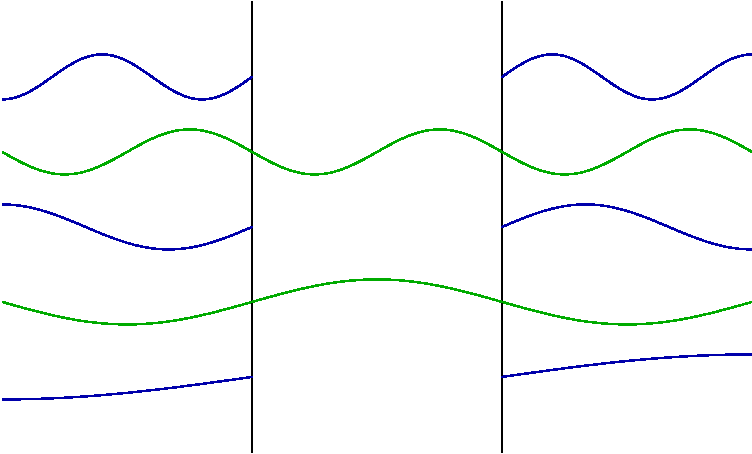
\includegraphics[width=6cm]{fig/intro/twoplanes_wave}
\caption[Allowed modes between parallel plates]
{Sketch of allowed modes between perfectly conducting plates. 
 Only waves with a half-integer number of wavelengths fit between the plates.
Blue modes are only allowed outside the plates, while green modes are allowed inside
and outside.  Modes have been vertically offset for clarity.  }
\label{fig:Casimir_sketch}
\end{figure}

The theory was extended by Lifshitz and coworkers to describe forces between dielectric half-spaces~\cite{Lifshitz1956,
Dzyaloshinskii1959,Dzyaloshinskii1961}.  This can recover the Casimir force between 
perfect conductors, and Casimir--Polder forces between atoms' and dielectric surfaces.  
We will sketch the derivation of the Lifshitz formula (which we will require later),
since this can naturally also compute the Casimir energy.

%  As intimidating as this expression is, it can be heuristically derived with
% relative ease via the ``argument principle''~\cite{vanKampen1968}.  
% In essence, since the Casimir energy is the sum of the vacuum energy over all modes, the energy can
% be written as a complex contour integral of the energy against a function with poles at the allowed 
% energies.  For two plates the allowed modes satisfy the Fabry-Perot condition,
% \begin{equation}
%   \Delta = 1 - r_1r_2 e^{2ik d}.
% \end{equation}


\subsubsection{Derivation of Lifshitz Formula}
\label{sec:lifshitz}
The Lifshitz formula for the Casimir energy can be found with an ingenious argument due to van Kampen\etal\cite{vanKampen1968}.
In its full generality, the Lifshitz formula gives the total energy for two planar dielectric bodies with dielectric constants $\epsilon_1,\epsilon_2$
separated by a medium with dielectric constant $\epsilon_3$.  
(This derivation parallels those is taken from \S 7.2 in Milonni~\cite{Milonni1994} and Ch.12 of Bordag\etal\cite{Bordag2009}.
A similar result emerges from the scattering approach as discussed by Lambrecht\etal\cite{Lambrecht2011}.)
The energy for the EM field in its ground state is 
\begin{equation}
  E = \sum_{\zeta}\sum_{k_x,k_y,\omega} \frac{\hbar\omega_k}{2},
\end{equation}
where the sum runs over all of the allowed modes for the particular arrangement of bodies.  
In this case, the  non-zero contribution to the Casimir effect comes from surface plasmon modes, which propagate along the interfaces
and decay exponentially away from the bodies.  
The sum over frequencies can be recast as a contour integral over complex frequency $\xi$, against a function $\Delta^{(\zeta)}$,
 whose poles occur at the allowed frequencies, with residue $\omega_k$:  
\begin{equation}
  E = \frac{L^2}{(2\pi)^2}\sum_{\zeta}\int_0^\infty dk_T\,k_T\oint d\xi\, 
  \frac{\hbar \xi}{2} \frac{1}{(2\pi i)\Delta^{(\zeta)}(\xi)}\frac{d\Delta^{(\zeta)}(\xi)}{d\xi},
\end{equation}
where the function $\Delta'(\xi)/[2\pi i\Delta(\xi)]$ is designed to have unit residue at the zeroes of $\Delta(\xi)$, 
and $k_T$ is the transverse wavenumber.  The factor of $L^2$ is accounted for by considering the energy 
per unit area.  
The energy can be simplified by integrating by parts leading to 
\begin{equation}
  \frac{E}{A} = \frac{\hbar}{16\pi^3 i}\sum_{\zeta}\int_0^\infty dk_Tk_T\oint d\xi \, \ln\Delta^{(\zeta)}(\xi).
\end{equation}
The most important modes are the surface modes, since these modes are sensitive to the position of the other body, where
these modes exponentially decay between the bodies.
The allowed frequencies for these modes must satisfy 
\begin{equation}
  r^{\zeta}_{13}r^{\zeta}_{23} e^{-2k_z d}=1,
\end{equation}
where $r^\zeta_i$ are the reflection coefficients for surface $i$ and polarization $\zeta$ and\
the wavenumber is given by $k_z=\sqrt{k_T^2-\epsilon(\omega)\omega^2/c^2}$.  The reflection coefficients
are given by 
\begin{equation}
  r\supTE_{13} = \frac{k_{z,1}-k_{z,3}}{k_{z,1}+k_{z,3}} \qquad 
  r\supTM_{13} = \frac{\epsilon_3k_{z,1}-\epsilon_1k_{z,3}}{\epsilon_3k_{z,1}+\epsilon_1k_{z,3}}.
\end{equation}
The frequency condition is suggestive of the requirement that accumulated round-trip phase 
(including reflections from both walls) is unity for
allowed modes (this interpretation is bolstered by considering the Casimir force between mirrors~\cite{Genet2003}).
This suggests choosing $\Delta(\xi) = 1-r^{\zeta}_{13}r^{\zeta}_{23} e^{-2k_z d}$, where the wavenumber $k_z$
and the reflection coefficients are functions of $\xi$.  

The complex contour integral can be split into two pieces: the integral over the right semi-circle 
is apparently independent of $d$, and can be ignored.  This leaves the integral along the imaginary 
frequency axis, $\omega=is$.  
It turns out Casimir effects are most naturally discussed along the imaginary frequency axis.  
Due to the causal nature of the dielectric response functions, the dielectric function is a 
smooth, real function on the imaginary axis.  This also means that the $z$-wavenumber is also real,
with $k_z=\sqrt{k_T^2+\epsilon(is)s^2/c^2}$, 
and that oscillatory functions like plane wave factors are replaced with real, decaying exponentials.  
Both of these features are extremely attractive for numerical methods, and so this is also
often used in numerical methods~\cite{Johnson2011}.

The Casimir energy between two dielectric half-spaces of permittivities $\epsilon_1, \epsilon_2$
separated by a gap of thickness filled with permittivity $\epsilon_3$ is given by 
\begin{align}
\frac{E}{L^2} =& -\frac{\hbar}{2\pi^2c^3}\int_0^\infty ds\, s^2 \epsilon_3
\int_1^\infty dp\,p\sum_{\zeta=\text{TE, TM}}\log\left[1 - r^{(\zeta)}_{13}r^{(\zeta)}_{23}e^{-2\sqrt{\epsilon_3}ps d/c}\right],
\label{eq:lifshitz}
\end{align}
where the electromagnetic reflection coefficients are given by 
\begin{align}
  r\supTE_{ij}  = \frac{\kappa_i-\kappa_j}{\kappa_i+\kappa_j},\quad
  r\supTM_{ij}  = \frac{\epsilon_j \kappa_i - \epsilon_i \kappa_j}{\epsilon_j \kappa_i + \epsilon_i \kappa_j},
\end{align}
and
\begin{equation}
  \kappa_i = \sqrt{p^2 + \epsilon_i/\epsilon_3-1}.
\end{equation}
following Zhou~\cite{Zhou1995}.
The variables have been adjusted to agree with Lifshitz original calculation, by defining 
\begin{align}
  k_T &= \frac{s}{c}\sqrt{\epsilon_3(p^2-1)}.
\end{align}
In general, this integral form is the simplest expression for the Casimir energy between dielectrics. 
% As intimidating as this expression may be, it is a necessary touchstone for later comparison, and it allows 
% us to examine the different scaling regimes at different distances.  
The perfect-conductor Casimir energy result (\ref{eq:Casimir_energy}) can be found by taking the strong-coupling limit,
 $r^{(\zeta)}_i\rightarrow 1$, and setting $\epsilon_3=1$.  and evaluating the integrals using 
\begin{equation}
  \int_0^\infty ds\,s^2 \int_1^{\infty} dp\,p \log[1 - e^{-2 s p d/c}] = -\frac{c^3 \pi^4}{360 d^3}.
\end{equation}
The Casimir--Polder results for interacting atoms can be recovered from the Lifshitz formula by taking the limit of dilute bodies,
$\epsilon \approx 1+\alpha n$, where $n\ll 1$ is the density, and $\alpha$ is the polarizability.

% This was further expanded on by Dzyaloshinskii\etal\cite{Dzyaloshinskii1959,Dzyaloshinskii1961} who
% showed the connection between Casimir force and the pair-wise van der Waals potentials.  
%This work is reviewed by McLachlan~\cite{McLachlan1963, McLachlan1963a}.  

The Lifshitz theory can be extended to account for dispersion and finite temperature.  
Some care is required in quantizing the electromagnetic field within dielectric media,
since due to the Kramers-Kr\"onig relations, the presence of dispersion implies dissipation.
% The usual approach to open-systems in quantum mechanics is to couple the system to a reservoir, 
% and integrate out the reservoir.  
However, it has been phenomenologically observed that one gets the correct answers by a direct substitution
$\epsilon(\vect{x})\rightarrow \epsilon(\omega,\vect{x})$.  This issue has in investigated more carefully in~
\cite{Barash1975,Rosa2010}, and justified by careful examination of the thermodynamic energy
and relation to the microscopic details of the medium.   

At non-zero temperature it is necessary to also include the effects of real thermally excited photons,
by accounting for the mean number of excited photons.
At inverse temperature $\beta=(\kB T)^{-1}$, for a 
frequency $\omega$, the mean number of photons is $\bar{n}(\omega) = \coth(\beta\hbar \omega/2)$.  
Note that $\coth(i x)$ has simple poles at $x=\pm n \pi$ for $n$ integer. 
Exactly the same style of argument can be used to find the thermal Casimir energy between dielectrics, 
but now due to the presence of $\coth(is)$, the integral over imaginary frequency picks up the residues of the integrand at the 
Matsubara frequencies $s_n:= 2\pi n/(\beta\hbar)$.
The resulting free energy per unit area is 
\begin{align}
  \frac{\mathcal{F}}{L^2} =& \frac{\kB T}{2\pi}{\sum_{n=0}^\infty}' s_n^2 \epsilon_3
  \int_1^\infty dp\,p\sum_{\zeta=\text{TE, TM}}\log\left[1 - r^{(\zeta)}_{13}(is_n)r^{(\zeta)}_{23}(is_n)e^{-2\sqrt{\epsilon_3}ps_n d/c}\right],
  \label{eq:lifshitz_finite_temp}
\end{align}
where the primed sum gives half the weight to the $n=0$ term, and all functions of frequency are evaluated at $s_n.$ 
At zero temperature, this result passes over to the previous one, 
by transforming the sum over frequencies into an integral.  This is the most general form of the Lifshitz
formula, and can recover all of the limiting behaviors at close distance, far field, and perfect conducting
media, and rarefied media.

\subsection{Physical Interpretation}

Casimir's original calculation vividly shows the importance of vacuum fields, and is said to show the reality 
of the vacuum field.  This is due to the emphasis given to the imposed boundary conditions,
which are emphasized over the matter that created the boundary conditions~\cite{Jaffe2005}.  
It is the author's opinion that the Casimir effect is best thought of as a long-ranged interaction between dielectric bodies 
mediated via the electromagnetic field~\cite{Jaffe2005, Rahi2009}.  This picture is also
analogous to the intuitive photon exchange picture used to explain the Casimir--Polder potential.
% This view makes the clearest connection to the underlying fundamental physics, rather than emphasizing idealized
% boundary conditions.
  Fig.~\ref{fig:electron-effective-interaction} shows a term contributing to the Casimir effect where 
electrons on different bodies interact with one another via the electromagnetic field.
  The solid lines should
be understood as the current operators for the electrons bound to a particular, separate media, while the 
wavy lines are the EM green functions describing the photon.  In fact, if summed over all such dipole ``bubbles'',
one can recover the full Casimir force results --- as was done by Dzyaloshinskii\etal in re-summing a field 
theoretic expansion~\cite{Dzyaloshinskii1961}.  
In that case the closed electron loops should be understood as current-current correlation functions,
$\langle j_\mu j_\nu\rangle$, where under linear response theory, this correlation function is related to the conductivity
tensor $\sigma_{\mu\nu}$~\cite{Kubo1957,Altland2011}.  The conductivity tensor is in turn related to the dielectric tensor, $\epsilon_{ij}$
via Ohm's Law $j_i=\sigma_{ij}E_j,$ which makes the connection between this condensed matter physics,
and the material functions used in the Casimir effect\footnote{
  This relationship was pointed out by Rahi\etal\cite{Rahi2009}, as a justification for their starting point
  in quantizing the electromagnetic field in media.}.

%\todo{Details of Kubo?}
% \comment{Effective interaction: expanding out perturbation theory leads to $\langle j_\mu j_\nu\rangle$
% correlation functions.  Via Kubo formalism for linear response, this is related to the conductivity
% tensor $\sigma_{\mu\nu}$, which is in turn related to the dielectric constant $\chi$}

 \begin{figure}
 \centering
 \begin{fmffile}{wall-wall}
% \begin{fmfgraph}(50,30)
%  \fmftop{t0,t1,t2,t3}
%  \fmfbottom{b0,b1,b2,b3}
%  \fmf{fermion,tension=0.5}{t1,v1}
%  \fmf{fermion,tension=0.5}{t2,v3}
%  \fmf{fermion,tension=0.5}{b1,v2}
%  \fmf{fermion,tension=0.5}{b2,v4}
%  \fmffreeze
% \fmf{photon,tension=0}{v1,v3}
% \fmf{photon,tension=0}{v2,v4}
% \fmf{fermion,tension=0}{v1,v2}
% %\fmf{fermion,tension=0,left}{v2,v1}
% \fmf{fermion,tension=0}{v3,v4}
% %\fmf{fermion,tension=0,right}{v4,v3}
% \end{fmfgraph}
\begin{fmfgraph}(50,30)
 \fmftop{t0,t1,t2,t3}
 \fmfbottom{b0,b1,b2,b3}
 \fmf{phantom}{t1,v1}
 \fmf{phantom}{t2,v3}
 \fmf{phantom}{b1,v2}
 \fmf{phantom}{b2,v4}
 \fmffreeze
\fmf{photon}{v1,v3}
\fmf{photon}{v2,v4}
\fmf{fermion,tension=0}{v1,v2}
\fmf{fermion,tension=0,left}{v2,v1}
\fmf{fermion,tension=0}{v3,v4}
\fmf{fermion,tension=0,right}{v4,v3}
\end{fmfgraph}
\end{fmffile}
\caption[Casimir Energy in terms of fundamental QED processes. ]
 {Casimir Energy in terms of fundamental QED processes.  The electrons are considered bound within their respective media,
 but still interact with electrons on other bodies by exchanging photons.  Any self-interactions are removed 
by renormalization via considering energy differences.  The effective interaction of the 
electron current with the field is described by the dielectric constant.}
\label{fig:electron-effective-interaction}
\end{figure}

\subsection{Comparison with other forces}

Casimir or van der Waals forces, are the dominant forces for electrically neutral bodies.  
However, they can be screened by other electrostatic forces in some circumstances, particularly if one is 
considering metal bodies~\cite{Lamoreaux2011,Bordag2009}.  
These electrostatic forces typically have a longer ranged force law than the Casimir effect, 
with a similar order of magnitude. 
In order to detect the classic Casimir force between conducting bodies, it is then necessary to carefully 
remove any stray background fields.  These arise from patch potentials (localized distributions of electric charge
on a conductors surface), stray charges, or adsorbed atoms.  

Note that while these electrostatic forces can be mitigated, the Casimir effect cannot be removed.  
The resulting power law potentials are relatively short-ranged power laws compared to the Coulomb potential 
between charged particles which decays $d^{-1}$. 
We will compare the size of the Casimir force to typical Coulomb energies that arise in experiments.
We will also compare the Casimir--Polder energy to the typical trapping potentials used to trap atoms.
  
% While the Casimir effect is short-ranged compared to the $d^{-1}$ Coulumb potential between charged particles.
% However, most bodies are electrically neutral and thus have no long-ranged Coulomb potential, whereas
% the Casimir effect applies even if the bodies have no net charge.  

For macroscopic bodies we can compare the Casimir energy for perfect 
metal conductors at a distance $d$ to the energy stored in the capacitance.
The Casimir pressure (force per unit area) is $P_{\text{Cas}}=\frac{\hbar c\pi^2}{240 d^3}$.
This can be can be compared to the energy in a parallel-plate capacitor (pg. 219 of \cite{Milonni1994}.)
For a parallel-plate capacitor, with surface charge density $\sigma$, the attractive force 
between the plates is $P_{\text{cap}}=\sigma^2/(2\epsilon_0)$.  For a parallel-plate capacitor filled with
vacuum, the capacitance is $C=A\epsilon_0/d = QV$, which implies $\sigma=Q/A=\epsilon_0V/d$.
The capacitive pressure is then $P_{\text{cap}}= \dfrac{\epsilon_0 V^2}{2d^2}$.  At a distance of $1\mu$m
this corresponds to a voltage of $17$mV.  
In experiments, voltages of this magnitude are observed from electrostatic sources~(Ch 18 and 19 of Ref.~\cite{Bordag2009}).

For conducting bodies, such stray potentials can emerge from variations in the work function
of the metal~\cite{Lamoreaux2011}.
If the Fermi surface dips below the surface of the metal, a localized electric charge can build up.
This is one of the dominant backgrounds in Casimir experiments, and must be subtracted off to extract the Casimir effect.
These various electrostatic potentials are randomly distributed and show a $d^{-1}$ power law
contribution to the force~\cite{Sushkov2011}, as opposed to the faster $d^{-2}--d^{-3}$ behavior expected
from the Casimir force.  

The typical Casimir--Polder energy scale can be estimated from dimensional considerations.
For a typical atom, with size $r=1\AA$, the dipole moment $d\sim er$.  The static polarizability
is then $\alpha\sim \sum_jd_j^2/(\hbar\omega_j)$.
The Casimir-Polder energy in the far-field is then
\begin{align}
  V\subCP &= -\frac{3\hbar c\alpha_0}{32\pi^2\epsilon_0 d^4}%\\
%  &= -\frac{3\hbar c e^2r^2}{32\pi^2\epsilon_0 \hbar\omega_0d^4}\\
%  &= -\frac{10^8 10^{-19}10^{-20}}{10^2  10^{-11} 10^{15}10^{-24}} eV\\
%  &= -\frac{10^{-31}}{10^{-19}} eV\\
  \approx -10^{-12}eV,
\end{align}
which corresponds to a frequency shift on the order of $10$kHz for a generic atom at 1$\mu$m.  
% In the near-field, it is necessary to shift over to the van der Waals energy, where the atom interacts
% with its image dipole.
In comparison, a far-off resonant light beam can create an all optical trap with a depth of $10^{-9} eV$
\footnote{Assume the atom is cooled down to the Doppler temperature, for which $E\sim\hbar\Gamma\sim 10^{-28}J\sim 10^{-9}eV$}
So at a distance of $1\mu$m from a surface, it may be possible to trap an atom, but at a tenth of that distance the Casimir--Polder
attraction would overcome the optical trapping potential.

%As comparison, a typical trapping potential using far detuned lasers is 
% As an example, atoms near a conducting surface can adsorb onto the surface, and form ionic bonds with a large dipole 
% moment.  This permanent dipole polarizes the atom, leading to an atttractive potential~\cite{McGuirk2004}.  
% The resulting potential can be written in terms of the atomic polarizability $\alpha$,
% \begin{equation}
%   V_{\text{ad}}(\vect{r}) = -\frac{\alpha_0}{2}|\vect{E}(\vect{r})|^2,
% \end{equation}
% where $\vect{E}$ is the field from the adatom dipole.  
% The electric field for a dipole at the origin of dipole moment $\vect{d}$ is 
% \begin{equation}
%   \vect{E}(\vect{r})=\frac{1}{4\pi\epsilon_0|\vect{r}|^3}[3(\vect{d}\cdot \hat{r})\hat{r}-\vect{d}]. 
% \end{equation}
% The square of the electric field is 
% \begin{equation}
%   |\vect{E}(\vect{r})|^2% =\frac{1}{(4\pi\epsilon_0|\vect{r}|^3)^2}
%   % [9(\vect{p}\cdot \hat{r})^2-6(\vect{p}\cdot\hat{r})^2+\vect{p}^2]
% =\frac{1}{(4\pi\epsilon_0|\vect{r}|^3)^2}  [3(\vect{d}\cdot \hat{r})^2+\vect{d}^2]
% \end{equation}
% So for order of magnitude estimates, the interaction potential is approximately
% \begin{equation}
%   V_{\text{ad}}(\vect{r}) \sim -\frac{\alpha_0}{2}\frac{1}{(4\pi\epsilon_0|\vect{r}|^3)^2}\vect{d}^2
% \end{equation}

\subsection{Different Distance Scaling Regimes}

The Casimir effect is important at distances around the resonant wavelengths of the atom or medium,
 which are typically on the order of $1\mu$m for optical transitions.  
The Casimir effect is typically computed in a long-wavelength or low energy limit where the constituents of the bodies can be treated 
as a continuum.
%This long-wavelength limit also corresponds to energies small compared to the binding energies of the bodies.
This approximation starts to break down when the distances between bodies approach the separation of the constituent atoms.
which is around $1\AA$, where exchange effects and other physics becomes important.
At the other limit, for distances beyond $100 \mu$m, the Casimir effect becomes too weak to detect.  

The distance scaling of the Casimir energy for bodies separated by a distance $d$, can be found by approximating 
the Lifshitz integral~(\ref{eq:lifshitz_finite_temp}) in certain limits.
%The differing scaling emerges by approximating the integrals in the Lifshitz formula~(\ref{eq:lifshitz_temperature}) in various limits.  
% The distance scaling depends on the nature of the bodies, and the how large the separation is in comparison to 
% relevant wavelengths in the problem.  
% For pairs of macroscopic slabs the energy scales as $d^{-2}$--$d^{-3}$, depending on the separation, 
% while the energy scales as $d^{-6}$--$d^{-7}$ for pairs of atoms.  
In particular, one must compare the separation of the bodies $d$ to the resonant wavelengths or frequencies of 
 of the interacting media.  
This requires some knowledge of the peak frequencies $\omega_A$ of the atomic polarizabilities $\alpha(\omega)$ or the dielectric
 function $\epsilon(\omega)$.  At nonzero temperature, there is another distance scale given by the thermal wavelength,
 $\omega_T=\kB T/\hbar$.  One can estimate the most important frequencies by examining $\alpha(is),\epsilon(is),e^{-2pd\xi/c}$
and approximating the integral in various limits. 

 In the near field or van der Waals regime, the separation of the bodies is less than any of the 
 resonant wavelengths for the bodies $d\ll \omega_A/c,\omega_M/c$.  In that limit $\epsilon(i\omega)$ serves to cut off 
 the frequency integral, and the exponential factor $e^{-2pd\xi/c}$
 is unity for all relevant frequencies.  In essence, the interaction is an instantaneous 
 dipole interaction between the media.  For example the atom-wall potential shows a $d^{-3}$ scaling. 

 In the retarded or Casimir-Polder regime, the atoms are much further than a resonant wavelength 
 $d\gg \omega_A/c,\omega_M/c$.  In that case the dominant contributions come at zero frequency, 
and the functions can be approximated with their static limit.
 This typically occurs for distances greater than a micron.
 In this far field regime, the potential typically decays more quickly.  For example, the  atom-wall
potentials shows a $d^{-4}$ scaling in this limit.

At even greater separations between the bodies is the thermal regime $d\sim \omega_T/c$, where the real photons excited by the 
 thermal field contribute significantly to polarizing the atom.  At room temperature, the thermal wavelength is
 $\lambda_T=\hbar c/(\kB T)~10\mu m$.  In this regime the potential falls off more slowly as $E\sim d^{-3}$,
 the same as the near-field van der Waals regime.  

\section{Overview of Casimir Experiments}
\label{sec:expt_review}

The Casimir effect has been measured in experiments, both for macroscopic bodies and atoms.
This section provides a brief overview of the broad categories of experiments where the Casimir effect is relevant,
and the challenges these experiments provide to theoretical and computational methods.    
The following is intended as a broad survey, since the full literature on the Casimir and Casimir--Polder 
effects is quite large.  

%Lamoreaux
\subsection{Experiments on Casimir Forces}

%\todo{Citation for this?}

Despite it's prediction in 1948, the Casimir effect proper proved quite difficult to directly measure.
Some early confirmations used the Casimir effect to explain the thickness of liquid helium film on 
the wall of its container~\cite{Sabisky1973,Dzyaloshinskii1961}.
In that case, helium satisfies the repulsive Casimir criterion and it is energetically favorable
to have helium between the vacuum and the walls.  
% An early indirect measurement was liquid Helium flowing up the walls of a container.  \todo{Citations!  Lifshitz/Dzyaloshinskii}
% Lifshitz and co-workers applied the Casimir pressure to explain the phenomenon of liquid helium
% flowing out of a jar.  
% The presence of the liquid helium crawling up the surface reduces the Casimir energy,
% between the vacuum and the sides of the jar, so the liquid helium experiences an attractive pressure up the walls.  

The Casimir effect was only precisely measured in 1997 by Lamoreaux~\cite{Lamoreaux1997}.   
%Lamoreaux's work spurred a large amount of experimental and theoretical work.  
This experiment measured the Casimir force between a sphere above a metal plate,
and measured the force via a torsion pendulum.  
This landmark experiment was closely followed by measurement by Mohideen\etal\cite{Mohideen1998}
using an atomic force microscope to measure the force in a sphere-plate geometry.  
The Casimir force has also been directly measured in a nanoelectromechanical (NEMS) system 
by Chan\etal~\cite{Chan2001}.  In this case, the Casimir force is detected by the modification it
makes to the frequency of a torsional oscillator suspended above a plate.  
The sphere-plate and oscillator geometries have the experimental advantage of removing the need to carefully
align the parallel metal plates. % Given the strength of the Casimir force it is hard to keep the plates exactly parallel,
% and separate, which is something that dogged early attempts to measure the Casimir force.
Despite the aforementioned difficulties, the Casimir force between parallel plates was measured precisely by Bressi\etal~\cite{Bressi2002}.  

The Casimir force is also important in applications of microelectromechanical systems (MEMS), 
as a source of stiction~\cite{Tas1996, Serry1998, Buks2001}.  This is particularly important
in free standing structures such as nano-oscillators.  %\todo{Comment on non-linear actuation blah?}
Given the Casimir force is an attractive potential, if parts of the device get too close to the substrate
they will permanently stick to one another, leading to device failure.  

Precisely measuring such a small force requires careful calibration of the measurements 
and removing systematic effects.  Reviews of these and other difficulties are available in Refs~(\cite{Lamoreaux2011, vanZwol2011, Bordag2009}).
Two of the primary experimental errors are due to 
patch potentials, and surface roughness.  The patch potentials are localized surface 
charge distributions, which due to the longer range Coulomb interaction must be subtracted off to extract the weaker
Casimir force~\cite{Sushkov2011}.  The fact that the thin metallic films and surfaces used in these 
experiments are not perfectly smooth is referred to as surface roughness, and is one of 
the main theoretical sources of error in these experiments.  
In addition, the optical properties of the surface must also be carefully characterized, since the 
optical properties of a coating can vary significantly.  Another difficulty in predicting the size of the 
Casimir effect is that the optical properties must be interpolated from data for other experiments~\cite{vanZwol2011}.

\subsection{Experiments on Casimir-Polder Forces}

Van der Waals and Casimir--Polder forces were first observed experimentally in molecules, 
which prompted the further development of theory to explain the effects.  
Beyond those early experiments, Casimir--Polder forces have also been measured precisely in more modern experiments  
using isolated atoms in experiments using atomic beams, cavity QED, and Bose-Einstein condensates.  

The first modern attempts at directly measuring the Casimir-Polder force used atomic beams 
near surfaces.  Sukenik\etal made the first modern attempt to measure the Casimir-Polder force~\cite{Sukenik1993}.
Their experiment passed a hot beam of atoms through an optical cavity and attempted to detect
the effect by the small phase-shift induced on the atoms.  Unfortunately, their measurement 
was not definitive.
More recent experiments by Perreault\etal\cite{Perreault2005}, and Lonig\etal\cite{Lonij2009} succeeded in measuring
the Casimir-Polder force with atomic beams.  These experiments passed an atomic beam past grating and 
detected the phase-shift by atom interferometry.  

The Casimir-Polder effect has also been observed in the context of a Bose-Einstein Condensate (BEC)
of ultra-cold atoms~\cite{Harber2005,Obrecht2007}.  % The BEC allows for precise distance control,
% and can be used in atom interferometry to detect small phase shifts.    
The atoms are confined to a harmonic trap, and can be brought near to a surface to probe the Casimir
force, where the Casimir force acts to shift the oscillation frequency of the harmonic trap in a position
dependent manner.  % These experiments were able to measure the Casimir--Polder force in the thermal regime,
% vary the distance of the atoms from the surface from $1\mu m$ up to 10 $\mu m$
% This technique was able to measure the Casimir force in the thermal regime, which
% is often difficult since the force is weak at those distance, but was accessible here due to the stability of the BEC.
% In this case it was ``easy'' to  to observe
% the cross over between the Casimir-Polder and thermal regimes.

The Casimir-Polder force is also important in developing atomic technologies.  
Atoms are an attractive platform for a number of reasons:
Each atom of the same species is identical; 
atoms have readily accessible, well-defined transitions that can be used to control their motion
, internal state and interactions; and atoms
have internal states that are long-lived, which would be important in storing information.

In recent years there has been a concerted push to develop technology that retains the appealing features 
of cold atoms in an architecture that can be scaled up to having large numbers of addressable atoms
~\cite{Kimble2008}.  
% There is a large effort across many fields to harness quantum technologies to develop scalable 
% quantum devices for computation and simulation of quantum systems
The desire to get strong-coupling between the atom and light fields, addressable qubits, and a scalable
architecture has pushed groups towards developing atomic traps that capture atoms close to dielectric surfaces.  
In this limit, the Casimir--Polder force is the dominant force, which can only be partially mitigated
by using laser fields to generate repulsive potentials.
In designing these new devices it is essential to compute and account for the Casimir-Polder force
the atom's experience when brought close to the dielectric surface.  

One direction that has been pursued is the atom-chip~\cite{Folman2000,Schneider2003,Salem2010},
where atoms are trapped within a few microns of the surface via a combination of lasers and magnetic fields from wires embedded in
the surface.  %The atoms are typically trapped within a micron of the surface.  
In most applications the Casimir effect acts as a lower bound on how close bodies can be brought 
to each other, which in turn limits the coupling strength, as well as how small devices can be made.
In the atom-chip example bringing the atoms closer than a micron lead to most of the atoms escaping the 
trap~\cite{Lin2004}.

Another direction that has been pursued is strong coupling of atoms to light via cavity 
quantum electrodynamics (QED).  
Kimble's group is developing microscopic dielectric waveguides to allow trapping, addressing and strongly interacting with  
single atoms in a scalable manner~\cite{Alton2011, Hung2013, Goban2014}.  In more recent work,
the Casimir--Polder potential is explicitly accounted for as part of the trapping potential~\cite{Goban2014},
and must be precisely computed.

\subsection{Current experimental directions}

Beyond directly detecting the Casimir effect, experiments are also moving in some directions worth highlighting,
since they are quite challenging for the theory to handle.  

% \subsubsection{Thermal Force and Material Model}

% There is a long-standing dispute between experimentalists on the best model to describe the 
% metals used in Casimir experiments.  In particular, should the metallic bodies be described by 
% the Drude or Plasma models?  These models provide the following dielectric constants for metals,
% \begin{align}
%   \epsilon_{\text{Drude}} &= 1+\frac{\omega_p^2}{\omega(\omega+i\gamma)}\\
%   \epsilon_{\text{plasma}} &= 1-\frac{\omega_p^2}{\omega^2},
% \end{align}
% where $\omega_p$ is the plasma frequency and $\gamma$ is the dissipation rate.
% The Drude model is consistent with Maxwell's equations, but some earlier experiments fit the plasma model 
% better.  This is also entangled in another debate over the role of the thermal Casimir effect, in particular what happens
% to the zero-frequency term from the TE polarization?  The Drude model has a simple pole at zero frequency,
% while the plasma model 
% These mattes are more a problem of reasoning than lacking theoretical or computational technology.  

% \subsubsection{Controversies over model}

% There are a couple as-yet unresolved issues in Casimir physics.
% Two of the leading experimental groups disagree on the appropriate model for the dielectric constant
% of a realistic metal.  
% Furthermore, there is also disagreement


%  Thermal casimir force
% Sushkov\cite{Sushkov2011}.
% Fight in literature over exact model used to describe metals at finite temperature.
% Drude vs plasma model.  
%  Lamoreaux favors Drude model, Capasso/Mohideen favours plasma model.

\subsubsection{Repulsive Casimir Effects}

Given that Casimir effects tend to enforce lower bounds for how close bodies can approach each other,
there have been a push to search for repulsive Casimir effects.  This would allow open the possibility
of trapping particles, and allow much smaller devices to be constructed.  
Unfortunately, these prospects are somewhat limited, due to requiring rare material properties.
From the Lifshitz formula, the sign of the force changes sign if $r_{12}r_{23}<0$.
This implies Casimir repulsion should be possible if $\epsilon_1<\epsilon_3<\epsilon_2$ over a broad range of frequencies.
This was experimentally demonstrated for a gold sphere immersed in bromobenzene above a silica plate
by Munday\etal\cite{Munday2009}.  However, this is method is little help for Casimir forces between
identical materials.  

Alternatively, the Casimir force is also repulsive for combinations of dielectric and magnetic materials~\cite{Boyer1974}.  
Given the strength of electric interactions over magnetic interactions in atoms, this spurred interest
in exploiting materials with strong magnetic responses~\cite{Kenneth2002}.  
Since these are relatively rare, there was some interest in exploiting metamaterials (arrays of micropatterned circuits with
effective magnetic response at certain wavelengths~\cite{Pendry1999}).  However, this was shown to be ineffective
for Casimir applications since the underlying metallic dielectric response dominates for the most important long wavelengths.
The metallic response implies an attractive potential, with the result that the overall Casimir effect would be attractive~
\cite{Ianuzzi2003comment,Rosa2008,Pirozhenko2008,Yannopapas2009}.  

While the preceding discussion emphasized varying materials for Casimir applications, it may 
be possible to exploit similar ideas for repulsive Casimir--Polder effects~\cite{Milton2011,Milton2012},
since the atom responds to a narrower range of frequencies.  In the far-field, the attractive dielectric
response may dominate, it might be possible to engineer near-field repulsion.  
These require an anisotropic response from the atom, which might be possible in the excited state.

Another way towards repulsive effects is by varying the geometry of the bodies.  
For example, the Casimir effect is repulsive in certain regimes for an elongated needle above a hole in a conducting plate~
\cite{Levin2010,Rodriguez2013}.  However, in this example the repulsion is unstable. 
In fact, it seems that it is impossible to get stable levitation for similar bodies via Casimir forces alone~\cite{Rahi2010}.

\subsubsection{Searches for new physics}

The Casimir force is also important for speculative searches for new physics on the millimeter to micron
scale~\cite{Dimopoulos2003, Bezerra2011}.  Since the new physics must be relatively short-ranged, 
it is typically modeled with a Yukawa potential, $V_{\text{Yuk}}=\alpha e^{-\lambda r}/r$,
which models the interaction with a new massive particle.    
On the micron scale however, the Casimir effect is the dominant interaction between neutral bodies,
 and must be carefully subtracted in an experimental procedure.
 Experiments then look for deviations from the expected Casimir effect, which means that the 
theory and experiment must be good agreement with one another.  
This approach has already been used to exclude regions of the parameter space for the hypothetical
Yukawa interaction~\cite{Obrecht2007,Bezerra2011}.  
Experiments searching for modifications of gravity typically employ a thin gold layer over
a density modulation.  The gold layer provides a common short-ranged Casimir interaction, while the 
a density modulation allows measuring variations due to gravity~\cite{Sorrentino2009, Geraci2015}.
Given the difficulties in cleanly measuring the Casimir force, this even more ambitious program has yet 
to yield results.  

% \subsection{Chemistry/Helium/Geckos?}

% \begin{enumerate}
% \item Geckos use the Casimir force \cite{Autumn2002}.
% \item Military applications to mimic at human scale. Cite 2015 paper.   
% \end{enumerate}


\section{Computational methods for Casimir Effects}
\label{sec:numerical_review}

Modern experiments require theoretical and computational methods
for the Casimir force that can account for a wide variety of material responses, anisotropies
and the ability to handle arbitrary shapes.  
% Although the Casimir force was explored by theorists before precision experiments were available,
% the advent of precision experiments and new technologies has spurred developments in 
% theoretical and computational methods.
% While early work focused on highly symmetric geometries 
% of bodies such as parallel planar bodies~\cite{Casimir1948,Lifshitz1956} or spheres~\cite{Boyer1968}, 
% current experiments require calculations for arbitrary shapes and arrangements of bodies, 
% which have realistic material properties.  
% This is a difficult task since the Casimir effect is a broadband phenomenon, depending on the whole 
% range of frequencies.  Furthermore, it depends sensitively on the geometry of the bodies involved, 
% and one must carefully renormalize the results to avoid infinite answers.  
For a simple, symmetric geometry (like perfectly conducting planes we used in Sec.~\ref{sec:CP_calc})
it is possible to write down tractable analytical expressions for
the Casimir energy based on expanding the field in mode functions.
%   However for general geometries 
% such an expansion may not be possible, or converge well.
However, for completely general geometries these requirements force one to adopt a general 
numerical approach to computing Casimir forces~\cite{Johnson2011}.
We will discuss three of these methods: the proximity-force approximation (PFA), the scattering
or fluctuating surface current approach, and the worldline method.

% \begin{enumerate}
% %\item Experiments spurred development of theory.  
% % \item Prior methods relied on mode-function expansion of fields, which is only possible
% % for simple geometries.  
% % \item Theory must account for material properties.  Surface roughness.  
% % \item Need general methods, tend to result in numerical integrals.
% % \item Crudest method available is the proximity force approximation.  
% % \item Analytical theory based on green function methods.  (Russian school, McLachlan, Schwinger)
% % \item Scattering approach.  
% % \item Worldline method.  
% \end{enumerate}

\subsection{Proximity Force Approximation}

The proximity force approximation (PFA) or Derjaguin approximation, is an uncontrolled approximation to
the Casimir force between generally shaped objects~\cite{Derjaguin1934,Blocki1977}.  
%\todo{Earlier citation is available}
The PFA treats each infinitesimal patch of the surfaces as if they were planar bodies,
and sums up the pair-wise interactions between different patches.
The PFA is assumed to be valid if the radius of curvature of the bodies $R$, is large relative to 
their separation $d$.  
For many years the PFA was the only practical general method of estimating Casimir forces in arbitrary geometries.
The PFA has the advantage of being straightforward to implement, and functions as an order of magnitude
estimate for the Casimir force for arbitrary geometries.
% It was used by Lamoreaux to estimate the Casimir force between the sphere-plate
% in his landmark experiments, where the radius of the sphere was indeed large compared to the separations explored. 

However it has some prominent limitations. First, it is only valid for vanishing curvature.
Second, the PFA assumes that the force can be found by integrating up
the pair-wise Casimir forces between each pair of surface patches.  This ignores the non-additivity
of the Casimir force.  Unlike the potential between electric charges where the total potential is
the sum of the pair-wise potential energies, the Casimir force for an arrangement
of bodies is not just the sum of the pair-wise energies.~(See \S{8.2} and \S{8.4} of \cite{Milonni1994})
As a crude justification, the Casimir energy involves the square of the electric field, which responds 
non-linearly as more bodies are added.  
% Finally, the PFA allows only for strictly attractive forces.  
% In contrast, the Casimir force can be repulsive, albeit under difficult to engineer circumstances 
% such as media with a strong magnetic response, or anisotropic media.
%\todo{PFA with frequency response for material?}

% \begin{enumerate}
% %\item Find first use?  Lamoreaux mentions usage.  Derjaguin?
% % \item Note problem with non-additivity. The PFA explicitly assumes that the force
% % can be found by adding up the pair-wise contributions from each surface patch.  
% % However, the Casimir force is a global phenomenon, and the total Casimir force
% % Useful if very limited curvature, or effectively approximate geometry as planar.  
% \item Only attractive.  (real electromagnetic casimir forces have possibility of 
% being repulsive, even if hard to realize in general.)
% \item ever extended to include material properties?
% \item Despite these limitations, the PFA is relatively straightforward to implement,
% and functions as an order of magnitude estimate for the Casimir force.  In the limit
% of vanishing curvature, the PFA converges to the correct Casimir force.  
% \end{enumerate}


\subsection{Scattering Approach}

The scattering approach is currently the only general method of computing 
electromagnetic Casimir forces between general media.  The scattering method 
is based on scattering techniques from classical electromagnetic theory and quantum mechanics~\cite{Rahi2009}.
%The roots of the scattering method in Casimir physics go back a number of decades.  
This method has been developed by a number of groups as an analytical method for general geometries~\cite{Emig2004, Lambrecht2006,
Kenneth2006, Emig2007,
MaiaNeto2008,Canaguier-Durand2012,Rahi2009}.  
% In Casimir physics, one is often interested in the scattered 
% EM field emanating from an object --- the renormalized interaction energies can be thought of as 
% emerging from this scattering.  
The Casimir energy can be written as 
\begin{equation}
  E = \frac{\hbar c}{2\pi}\int_{0}^\infty d\xi \log\det[\mathbb{M}\mathbb{M}^{-1}_{\infty}]
  \label{eq:scattering}
\end{equation}
where $\mathbb{M}$ is the scattering matrix describing scattering between the free modes of the electromagnetic
field induced by the presence of bodies, and $\xi$ is the imaginary frequency~\cite{Rahi2009}.
The energy is renormalized via $\mathbb{M}^{-1}_\infty$,
which is the scattering matrix as the bodies are removed to spatial infinity, this basically removes any
coupling between bodies and serves to remove any self-interactions. 
The indices of these matrices run over the labels of the possible modes (such as wavelength, polarization, mode origin for different bodies).
%Since different bodies have different shapes, it is necessary t be able to transform basis.  
Derivations similar to the argument principle used in Sec.~\ref{sec:lifshitz} can be applied to describe the scattering between modes,
--- instead of reflection coefficients for a surface, one considers the full scattering matrix for each body,
where matrix indices run over the labels (such as wavenumber, polarization) for the modes.
This has been applied for two-body systems such as realistic mirrors~\cite{Lambrecht2006}, surface roughness, 
and spheres and planes~\cite{Canaguier-Durand2012}.   
This subclass of these methods rely on scattering between mode functions suited to analytical expansions,
 and while they in principle offer a general purpose numerical method, 
the simulations may be slow to converge if the choice of basis functions is poorly suited to the actual
geometry required.  

The Johnson group at MIT has developed a formulation of the scattering method that is better suited to numerical 
applications for piece-wise constant media~\cite{Rodriguez2007,Rodriguez2007a, Rodriguez2009,Reid2009,Reid2011, Reid2013}.  
% Instead of describing the scattering from one mode into another, one can describe the scattering 
% locally at each patch of a surface.  
% The scattering between objects is described by coupling different surface patches together via the
% free-space Green functions.  
% This has justification from the Surface Integral Equations used in classical electromagnetism 
% ~\cite{Stratton1941}, and a variant on Green's theorem~\cite{Emig2004},
% where one can describe the field in each region by its free-space analogue, and couple it along the surface.
% (At the level of perturbation theory where the Casimir effect is computed, the photon Green function 
% can be described by its classical counterpart.)
% This method has also been able to leverage the development of classical EM solvers to the Casimir problem~\cite{Johnson2011}.
The fluctuating-surface-current formulation is a general method for computing Casimir
energies for piece-wise continuous linear dielectric and magnetic media~\cite{Reid2009,Reid2011, Reid2013}.  
In essence the method calculates the interaction between electric and magnetic surface currents 
on different bodies, mediated by the electromagnetic field.  Mathematically this is derived 
from a path integral for the electromagnetic field, where the fields are restricted to obeying EM boundary conditions at the 
surfaces via functional $\delta$-functions (simpler boundary conditions were handled in this fashion in
~\cite{Bordag1985,Li1991}).  The $\delta$-functions introduce fields 
bound to the surfaces, which can be interpreted as surface currents flowing to enforce boundary conditions.
After integrating out the EM field in the interior and exterior regions, 
these surface currents interact with one another via the electromagnetic Green function.
Since the method assumes piece-wise, homogeneous media and enforces EM boundary
conditions, it is the relatively simple homogeneous EM Green function that appears in these expressions.
These surface integrals are then discretized by splitting the surface into a finite number of patches.
All of the surface currents can then be integrated over, leaving a functional determinant analogous to Eq.~(\ref{eq:scattering})
where now the matrix elements $\mathbb{M}$ describe the coupling between different surface-patches induced
by the Green function.  (An expanded presentation is given in App.~\ref{app:scattering}.)

Numerically, this method comes down to computing the determinant of a large matrix, which is 
an intensive operation.  If a matrix has $N$ non-zero entries, the determinant for a dense matrix requires $\order(N^3)$ operations.
While it is possible to parallelize computing the determinant~\cite{Beliakov2013}, this is difficult.
However, for a sparse matrix system, it may be possible to make this relatively efficient 
and only require $\order(N\log N)$ operations~\cite{Reid2009}.
Since each frequency $\xi$ contributes independently, the integral over $\xi$ could be
trivially parallelized, but this may only offer relatively little parallelization for some problems.

The fluctuating-surface-current method has been used to 
for example describing the energy dependence of tetrahedral nanoparticles, capsules, and other  
geometries~\cite{Reid2009,Reid2011,Rodriguez2010}.  It has also been used to find cases 
where the Casimir force is repulsive due to geometric effects~\cite{Levin2010}, although the repulsion
is not stable~\cite{Levin2010,Rodriguez2013} .  
The scattering method has also been used in the design of atomic traps near dielectric waveguides, where the Casimir--Polder
force is an essential component of the trap~\cite{Hung2013}.  

As we noted, the scattering method is the only available general method for computing Casimir effects.
However, it is useful to have multiple methods with different computational properties
and biases, particularly when extending calculations to unexplored domains.  We now turn to the worldline
method which offers a very different picture and numerical method.  

\section{Path Integrals}
\label{sec:feynman_path_integral}
In order to discuss the modern methods of computing the Casimir effect it is necessary to introduce
the path-integral.  The path integral was originally developed by Richard Feynman as an alternative 
formulation of quantum mechanics~\cite{Feynman1948,Feynman1965}.
In the path integral, the probability amplitude for a particle to propagate from one position to another,
is given by the sum over \emph{all} possible paths between the points.
(In fact the path integral can be derived as the propagator from more traditional operator quantum mechanics~\cite{Sakurai1994}.)
Each path is weighted with a phase $e^{iS[x(t)]/\hbar}$ where $S[x(t)]$ is the classical action for the path.
For a free particle, the allowed paths are Brownian motions, or diffusive in nature.  

    Path integrals have been used extensively in a wide range of theoretical physics~\cite{Kleinert2012}.
    While offering an intuitive picture of quantum mechanics, they are much harder to use 
    than typical operator mechanics for anything other than the simplest problems~\cite{Feynman1965}.
    However, path integrals form a natural basis for quantum field theories, where they offer a relativistically covariant
    quantization procedure that naturally accounts for the gauge symmetries 
    that underlie the Standard Model of particle physics~\cite{Brown1994,Srednicki2008}.
    % In these field theoretic path-integrals, the integral runs over
    % all possible field configurations connecting the initial and final states, and some care is required
    % to handle the redundant degrees of freedom implied by gauge invariance~\cite{Faddeev1991}.

    Path-integrals have also been used in mathematics and statistics to describe stochastic 
    processes~\cite{Kac1949,Durrett1996, Karatzas1991}.  Rather than solving the Schr\"odinger equation, 
    this path integral is solves a diffusion equation --- this effectively passes over to ``imaginary time'',
    since after the Wick rotation which replaces, $t\rightarrow -i \tau$, the Schr\"odinger equation is a diffusion equation.
    This mathematical path integral weights each path by $e^{-S_{E}[x]}$, where $S_E$ is the real-valued Euclidean action for the path.
    In this form the path-integral has clearer convergence properties, 
    since the paths are weighted by real, decaying exponentials, as opposed to the oscillatory integrals
    in Feynman's path integral.  

    % The path-integral is one way to view stochastic processes, along side stochastic differential
    % equations and diffusion or Fokker-Planck equations. 
    % The path-integral is an infinite dimensional integral, which is the solution to an associated 
    % diffusion equation.  One can randomly sample from the 
    % dominant portions of the integral via Monte Carlo numerical methods.  These random sample paths can
    % in turn be described by a stochastic differential equations.  %\todo{Gardiner citation for SDE-> PDE}
        
    Path integrals underlie most of the work carried out in this thesis: we will use path-integrals
    to quantize the electromagnetic field, and the worldline method relies heavily on path integrals.
    In addition, we will use the connection between path-integrals and diffusion equations
    to verify analytically that the worldline path integral gives the correct results, and enhance our numerical
    calculations.  Considering their importance to this thesis, we will 
    now derive Feynman's path integral, which will serve as a prototype for all of the path integrals
    that follow.  (Our derivation follows the simple one given in Sakurai~\cite{Sakurai1994}.)
    % They have even been used in studying quantum chaos---the study of the quantum analogues 
    % of classically chaotic systems~\cite{Gutzwiller1990}.  In the semiclassical limit
    % where the classical action $S[x(t)]$ is large, the path integral for a chaotic system
    % can be approximated by only considering paths with periodic orbits.  %\todo{Gutzwiller trace formula citation}

    \subsubsection{Derivation of Feynman's Path Integral}

    Let us consider the quantum mechanical treatment of a particle in a time-independent potential $V(\vect{x})$, with Hamiltonian 
    \begin{equation}
      \op{H} =  \frac{\op{\vect{p}}^2}{2m} + V(\op{\vect{x}}),
    \end{equation}
    where the position and momentum operators obey the following commutation relations,
    \begin{gather}
      [\op{x}_i,\op{p}_j] = i\hbar\delta_{ij}\qquad      [\op{x}_i,\op{x}_j] = [\op{p}_i,\op{p}_j]=0,
      \label{eq:commutation}
    \end{gather}
    with resolutions of the identity,
    \begin{gather}
      I = \int d^Dx |\vect{x}\rangle\langle\vect{x}| = \int \frac{d^Dp}{(2\pi\hbar)^D} |\vect{p}\rangle\langle\vect{p}|,
      \label{eq:identity}
    \end{gather}
    and state overlap
    \begin{equation}
      \langle \vect{x}|\vect{p}\rangle = e^{i\vect{p}\cdot\vect{x}/\hbar}.
      \label{eq:overlap}
    \end{equation}

    In quantum mechanics, the amplitude for a particle starting at $x_i$ at time $t=0$, and propagating
    to $x_f$ at time $t$ is given by 
    \begin{equation}
      \langle x_f,t| x_i, t_0\rangle = \langle x_f| e^{-i\op{H}t/\hbar}|x_i\rangle.
    \end{equation}
    The amplitude to propagate from $x_0$ to $x_f$ can be developed into a path integral in a number of steps.
    First, split the evolution operator into $N$ pieces, and insert $(N-1)$ resolutions of the $\vect{x}$-identity 
    and $N$ resolutions of the $\vect{p}$-identity between    the pieces
    \begin{align}
      \langle \vect{x}_f,t_f| \vect{x}_i, t_0\rangle % &= \int \prod_{k=1}^{N-1} d^Dx_k 
      % \langle \vect{x}_f|e^{-i\op{H}\Delta t/\hbar}|\vect{x}_{N-1}\rangle
      % \langle \vect{x}_{N-1}|e^{-i\op{H}\Delta t/\hbar}|\vect{x}_{N-2}\rangle
      % \cdots \langle \vect{x}_1|e^{-i\op{H}\Delta t/\hbar}|\vect{x}_{0}\rangle\\
      &=\int \prod_{k=1}^{N-1} d^Dx_k \prod_{j=0}^{N-1} \frac{d^Dp_j }{(2\pi\hbar)^D}
      \langle \vect{x}_N|\vect{p}_{N}\rangle\langle\vect{p}_{N}|e^{-i\op{H}\Delta t/\hbar}|\vect{x}_{N-1}\rangle\nonumber\\
      & \hspace{0.5cm}\times\langle \vect{x}_{N-1}|\vect{p}_{N-1}\rangle\langle\vect{p}_{N-1}|e^{-i\op{H}\Delta t/\hbar}|\vect{x}_{N-2}\rangle
      \cdots \langle \vect{x}_1|\vect{p}_1\rangle\langle \vect{p}_1|e^{-i\op{H}\Delta t/\hbar}|\vect{x}_{0}\rangle
    \end{align}
    where $\Delta t:=t/N$, and we have introduced $x_N=x_f, x_0=x_i$. 
    At this point we can note the basic structure: the total amplitude for 
    the particle to propagate from $x_0$ to $x_f$ is the product of the amplitudes to propagate 
    from one point to the next, with the total amplitude being the integral (or sum) summed over 
    such paths.  
    Each infinitesimal time evolution operator can factored into a kinetic and potential piece, 
    \begin{equation}
      e^{-i\op{H}\Delta t/\hbar} = \exp\left(-i\frac{\op{p}^2}{2m\hbar}\Delta t\right)
      \exp\left(-iV(\op{x})\Delta t\right)+\order(\Delta t^2),
    \end{equation}
    where the corrections due to splitting and factorizing the exponential operator are higher order 
    in $\Delta t$.  
    (In general, it is crucial to consistently carry out all expansions in path-integrals to $\order(\Delta t)$.  
    % For example, in path integrals in curved space this often requires working to high order in $\Delta x$, 
    % and exploiting the equivalent of the Ito rule $dx^2=dt$~\cite{deWitt1957,Kleinert2012,Grosche1998}.
    )

    At this point, the position and momentum operators can be replaced by their eigenvalues, and the
    state-overlap can be used to write,
    \begin{align}
      \langle \vect{x}_f,t_f| \vect{x}_i, t_0\rangle 
      % &= \int \prod_{k=1}^{N-1} d^Dx_k \prod_{j=0}^{N-1} \frac{d^Dp_j }{(2\pi\hbar)^D}
      % \nonumber\\
      % \prod_{n=0}^{N-1}\bigg[\langle \vect{x}_{n+1}|\vect{p}_{n+1}\rangle
      % \langle\vect{p}_{n+1}|e^{-i\vect{p}^2_{n+1}\Delta t/(2m\hbar)}
      %   e^{-iV(\vect{x}_n)\Delta t/\hbar }|\vect{x}_{n}\rangle\bigg]\\
        &= \int \prod_{k=1}^{N-1} d^Dx_k \prod_{k=1}^{N-1} \frac{d^Dp_k }{(2\pi\hbar)^D}\nonumber\\
      &\times\bigg[\prod_{n=0}^{N-1}  e^{-i\vect{p}^2_{n+1}\Delta t/(2m\hbar)}     e^{-iV(\vect{x}_n)\Delta t/\hbar }
      e^{i(\vect{x}_{n+1}-\vect{x}_n)\cdot\vect{p}_{n+1}/\hbar}\bigg].
    \end{align}
    Since the momentum integrals are Gaussian, they can be straightforwardly evaluated
    \begin{align}
      \langle \vect{x}_f,t_f| \vect{x}_i, t_0\rangle 
      % &= \int \prod_{k=1}^{N-1} d^Dx_k \prod_{k=0}^{N-1} \frac{d^Dp_k }{(2\pi\hbar)^D}
      %   \prod_{n=0}^{N-1}\bigg\{  \exp\left[-\frac{i\Delta t}{2m\hbar}\left(\vect{p}_{n+1}  
      %       -\frac{m}{\Delta t}(\vect{x}_{n+1}-\vect{x}_n)\right)^2\right]\nonumber\\
      %   &\hspace{6cm}        \times \exp\left[ \frac{i m }{2\hbar\Delta t}(\vect{x}_{n+1}-\vect{x}_n)^2-\frac{i\Delta t}{\hbar}V(\vect{x}_n)\right]\bigg\}\\
        &= \int \prod_{k=1}^{N-1} d^Dx_k 
        \prod_{n=0}^{N-1}\bigg[\bigg(\frac{ m }{2\pi i\hbar\Delta t}\bigg)^{D/2}
        e^{i m (\vect{x}_{n+1}-\vect{x}_n)^2/(2\Delta t)}e^{ -iV(\vect{x}_n)\Delta t/\hbar}\bigg]\\
        &= \mathcal{N}\int D\vect{x} 
        \exp\left\{\frac{i}{\hbar}\int_{0}^{t} dt'\,\left[ \frac{m}{2} \dot{\vect{x}}^2-V[\vect{x}(t')]\right]\right\},
    \end{align}
    where in the final line we have taken the continuum limit, replacing $(\vect{x}_{n+1}-\vect{x}_n)/\Delta t
    \rightarrow \dot{\vect{x}}, \sum_n\Delta t f(n\Delta t) \rightarrow \int dt f(t)$, and introducing 
    $D\vect{x} = \prod_{k=1}^{N-1}d^Dx_k$.  The phase in exponent is the classical action for a particle
    in a potential.  Paths with the same phase will add together constructively, while 
    paths in regions where the phase is quickly varying will cancel one another out.  
    This leads to the classical limit where only the paths of stationary phase where $\delta S[x(t)]=0$
    contribute.

    % One can think of the integral as summing over all possible paths $\vect{x}(t)$
    % between points $x_0$ and $x_f$ weighted by their classical action.  This also suggests a number 
    % of semi-classical expansions, such as considering the limit when $\hbar\rightarrow 0$ to derive 
    % the classical limit, or in work on chaotic systems~\cite{Gutzwiller1990}.

    In this thesis, this simple type of derivation will be all we require.  We 
    will often work with the imaginary time version, which replaces the oscillating exponentials with
    decaying exponentials.  
    The extension to field path-integrals over fields is straightforward: the field $\phi(\vect{x})$ 
    is described by its value at finitely many points $\phi(\vect{x}_k)$, and one integrates over the field values at these 
    points.  At the end of the calculation, one lets the spacing between grid points go to zero, 
    and the size of the grid extend to infinity.  
    We will also only need to consider Gaussian path integrals, of the type considered here.  
    In a later chapter we will extend this derivation to include sources.

\section{Scalar Worldline Casimir Energies}
\label{sec:dirichlet_worldline}
The worldline method is an alternative method for computing Casimir energies.
The worldline method is a descendant of the scalar electrodynamics 
Feynman explored~\cite{Feynman1950}, where the effect of a quantum
field is described by summing over the paths of a virtual particle interacting with the other bodies. 
The worldline method was later developed as an alternative method for 
carrying out general quantum field theory calculations in terms of single particle 
quantum mechanics~\cite{McKeon1993, Strassler1992,Schubert2001}.  
% The worldline method is heavily based on Feynman's path-integral method, where the amplitude
% for a particle to move from one position to another is the sum over all paths between the positions,
% where each path acquires a phase proportional to the classical action for that path~\cite{Feynman1948,Feynman1965}.
The basic insight of the worldline method is that for one-loop effective actions, 
the field path integral calculation can be recast in terms of the particle path
 integral for particles traveling in closed space-time paths.
  Higher order loop calculations can also be carried out with more particles, 
and gauge fields can also be treated~\cite{Schubert2001}.
For example, the worldline method has been used to compute relativistic
field effects for quantum electrodynamics (QED) such as the Lamb shift~\cite{Schmidt1995},  
It has also been used as a numerical algorithm for computing these relativistic QED effects~\cite{Mazur2014}---
however, these methods were developed for free-space interactions at high energy, rather than the 
low energy Casimir phenomena we desire to describe.  

The worldline method was first used to compute scalar Casimir energies by Gies\etal~\cite{Gies2003,Gies2006, Gies2006a}.
The scalar worldline method has been extended to finite temperatures~\cite{Klingmueller2008},
 used to study the torsion of inclined planes~\cite{Weber2009},
and forces in the sphere-plane and cylinder-plane geometries~\cite{Weber2010, Weber2010a}.  
In these non-trivial geometries the worldline method has also been used to examine the failure of the proximity force approximation.
More recent work has focused on computing the stress-energy tensor~\cite{Schafer2012, Schafer2016},
with a view to exploring how the Casimir energy violates certain energy conditions (violations of which are required for certain exotic physics).

The scalar worldline is also related to some semi-classical expansions for the Casimir energy.  
In particular, it is a direct numerical method for computing the so-called optical path integral
\cite{Scardicchio2005, Scardicchio2006}.  The sum over intersecting paths is also reminiscent 
for the semi-classical approach to the Casimir force by Schaden and Spruch\cite{Schaden1998} that evaluates 
the Casimir energy by summing over all periodic orbits of light.  This latter work is particularly 
related to other work on the semiclassical limits of path integrals involving chaos~\cite{Gutzwiller1990}.
Both of these approximate techniques rely on a path integral expression for the Casimir energy that approximates electromagnetism as a
scalar field, and the worldline provides a general purpose way of evaluating those path integrals.   

The worldline method has also been applied to the Casimir piston, where there are interesting geometric effects
based on the geometry of the piston~\cite{Schaden2009,Schaden2009a}.
Most of this work is for idealized surfaces that imposed Dirichlet boundary conditions, but 
there has also been some effort to extend the worldline method to account for Neumann boundary
conditions~\cite{Fosco2010}.  To date there has only been speculation on how to extend the 
worldline method to electromagnetism~\cite{Aehlig2011}, which only considered perfect conductors,
and did not have concrete, correct results.    

% \begin{enumerate}
%   \item Semi-classical approach to Casimir force via trace formula~\cite{Schaden1998}
%   \item Also the optical path-integral.
% \end{enumerate}

% We consider a scalar field coupled to a background potential $V(\vect{x},t)$.  This potential
% embodies the location of the bodies we are considering.  % Starting from the classical action,
% we will derive the Hamiltonian for the fields, and then compute the quantum partition function.  
% The partition function can be written as a path-integral, which is readily evaluated as a functional
% determinant.  Ultimately we want the free energy, which can be further converted into a path integral
% for a fictitious single-particle.  This single-particle path integral forms the basis of the numerical
% world line method.   
\subsection{Derivation of the Scalar Casimir Worldline Path Integral}
We now introduce the basic scalar worldline method, to discuss its positive features and limitations. 
(We will use terminology and scaling of dimensions in common with our later work, rather than the 
choices used in the original papers by Gies\etal.)  

\change{See also Ch 20 of Steck's Quantum Optics notes for an alternative perspective on this work, including
some of the analytical techniques we will use later.}


Consider a scalar field $\phi(\vect{r},t)$, interacting with a background potential $V(\vect{r},t)$.  
The action for the field $\phi$ is given by 
\begin{equation}
  S = \int_0^T dt \int d\vect{r} \cL = \int_0^T dt \int d^{D-1}\vect{r} 
  \left[ \frac{1}{2c^2}(\partial_t\phi)^2-\frac{1}{2}|\nabla\phi|^2-V(\vect{r},t)\phi^2\right],
\end{equation}
where $V(\vect{r},t)$ defines the surfaces of the interacting objects
\begin{equation}
  V(\vect{r}) := \lambda \sum_r \delta[\sigma_r(\vect{r}-\vect{R}_r)],
\end{equation}
where $\lambda$ is the coupling constant, $\sigma_r(\vect{r})=0$ marks the locations of the surfaces, 
and $\vect{R}_r$ marks the center location of each body.
In most work on scalar worldlines, the coupling constant $\lambda$ is taken to infinity, 
which corresponds to imposing Dirichlet boundary conditions on the surfaces. 
For planar geometries, this recovers electromagnetic Casimir results for idealized perfect conductors.  

From the Lagrangian, one can find the Hamiltonian and quantize the theory.
% (While this is a somewhat length procedure, it is the clear formal procedure for quantization,
%  and useful to follow in cases where there may be ambiguities).
The momentum conjugate to $\phi$ is given by
\begin{equation}
  \Pi := \frac{\delta \cL}{\delta(\partial_t\phi)} = \frac{1}{c^2}\partial_t\phi,
\end{equation}
where $\frac{\delta}{\delta f(t)}$ denotes the functional derivative with respect to $f(t)$.    
The Hamiltonian is then given by
\begin{align}
  H &:= \int d^3r\,(\Pi\partial_t\phi -  L)= \int d^3r\,\bigg[\frac{\Pi^2}{2} + \frac{1}{2}(\nabla\phi)^2 +V(\vect{r},t)\phi^2\bigg].  
\end{align}
We are now in a position to quantize the theory by promoting the classical fields to quantum operators, 
$\phi\rightarrow \op{\phi},\, \Pi\rightarrow\op{\Pi}$.
The fields can be promoted to operators with equal-time commutation relations
\begin{equation}
  [\op{\phi}(\vect{r},t),\op{\Pi}(\vect{r'},t)] = i\hbar \delta(\vect{r}-\vect{r'}).
\end{equation}
In exactly analogous fashion to quantum mechanics, the overlap between states is given by 
\begin{equation}
  \langle \phi|\Pi\rangle = \exp\bigg[\frac{i}{\hbar}\int d^3r \phi(\vect{r})\Pi(\vect{r})\bigg].
\end{equation}

We can compute physical quantities of interest such as Casimir energies and forces
by taking suitable derivatives of the partition function. 
The quantum partition function for the field is 
\begin{equation}
  Z = \tr[ e^{-\beta\op{H}}] = \int d\phi \langle \phi| e^{-\beta \op{H}}|\phi\rangle,
\end{equation}
the trace is evaluated over the complete set of field states.  
It is actually more useful to carry out calculations with the free energy $\mathcal{F}=-\kB T \log Z$.
In classic path-integral fashion the exponential operator can be split into $N$ pieces, and resolutions of the identity
in both fields and conjugate-momentum fields can be inserted between each piece.  

% \begin{align}
%   Z &= \int d\phi_0\prod_{n=1}^N d\phi_n \langle \phi_n| e^{-\Delta \beta \op{H}}|\Pi_n\rangle
%   \langle\Pi_n| \phi_{n-1}\rangle
% \end{align}
After integrating out the momentum fields, the partition function can be written as a
Euclidean Path integral
\begin{equation}
  Z = \int D\phi \exp\left\{-\int_0^{\hbar\beta c} d\tau \int d^3r
    \left[ \frac{1}{2}(\partial_\tau\phi)^2+\frac{1}{2}(\nabla\phi)^2+V(\vect{r})\phi^2\right]\right\},
\end{equation}
where $\tau=\beta\hbar c$.  The partition function can be cast into a more suggestive form
by integrating by parts in the exponential integrand, 
\begin{equation}
  Z = \int D\phi \exp\left\{-\int_0^{\hbar\beta c} d\tau \int d^3r\,\phi(\vect{r},\tau)
    \left[-\frac{1}{2}\partial_\tau^2-\frac{1}{2}\nabla^2+V(\vect{r})\right]\phi(\vect{r},\tau)\right\},
\end{equation}
where the surface terms can be discarded by assuming the fields tend to zero at spatial (and temporal)
infinity.% \comment{Actually need frequencies for periodic functions.  Especially for finite temperature,
% dispersion.  Will discuss more carefully later.}

The functional integral over $\phi$ is Gaussian and can be formally evaluated immediately as a 
functional determinant, since the differential operator is positive operator.  
Some care is required in regularizing such infinite determinants.
This is done in analogy with finite dimensional Gaussian integrals.  
The fields can be considered as only being evaluated on a finite lattice of space-time points,
with the lattice also having a finite extent which bounds all bodies.  
The gradient operators can be treated via their finite difference approximations, 
which can be thought of as sparse matrices.
For example, $\partial_x^2\phi(x_k) \approx [\phi(x_k+\Delta)-2\phi(x_k)+\phi(x_k-\Delta)]/\Delta^2$
In that case the partition function is a large, finite Gaussian integral of the form, 
\begin{equation}
  Z_{\text{reg}} = \int d\phi_k\exp\left\{-\sum_{j,k}\Delta \tau (\Delta x)^{D-1}\phi_k A_{jk}\phi_j\right\}.
\end{equation}
where the labels over positions have been labeled with indices and the matrix $A$ represents the differential
operator.  
This regularized expression can be integrated, under the assumption that the eigenbasis of $A$ can be found, i.e.
where $A_{jk}\psi^{(n)}_k=\lambda_{(n)}\psi^{(n)}_k$.  In that case, each Gaussian integral decouples and the 
regularized partition function can be written as 
\begin{equation}
   Z_{\text{reg}} = C \prod_k \lambda_{(n)}^{-1/2} = C \det[A],
\end{equation}
where the determinant is understood to be the product of the eigenvalues of the operator $A$.
The limit of an arbitrarily large volume, and lattice resolution can be taken after integration.

In an analogous fashion, one can formally evaluate the partition function path integral as a 
functional determinant, 
\begin{equation}
  Z \propto {\det}^{-1/2}\left[-\frac{1}{2}\partial_\tau^2-\frac{1}{2}\nabla^2+V(\vect{r})\right].
\end{equation}
% The original computations for the worldline method stressed computing the quantum effective
% action for the scalar field.  This yields essentially the same expression.  This expression has
% also retained a factor of $2$ on the gradients --- this will simplify the representation of the 
% worldline path integral.
The proportionality is due to an additional (infinite) normalization constant, which will
be divided out in the renormalization process.  
The free energy for the interacting field can be written as 
\begin{equation}
  \mathcal{F} = -\kB T\log Z = \frac{1}{2}\kB T 
\log\det\bigg[-\frac{1}{2}\partial_\tau^2-\frac{1}{2}\nabla^2+V(\vect{r})\bigg]+C,
  \label{eq:free-energy-det}
\end{equation}
where $C$ is a constant.  
As it stands this functional determinant is divergent, but finite results can be found by subtracting off the 
free energy when the bodies are removed to spatial infinity.  Physically this corresponds to 
computing energy differences between different configurations of bodies.  % The renormalization also cancels off 
% the infinite constant normalization factors.  
The renormalized free energy can now be converted into a single-particle path integral via some formal 
manipulations.  First, we will use the identity $\log\det A=\tr\log A$, which can be readily
verified for positive finite matrices.  
\begin{align}
  \log\det A &= \log\prod_j \alpha_j
  =\sum_j \log\alpha_j
  = \tr\log A,\label{eq:log-det}
\end{align}
where we used the facts that the trace and determinant of a matrix are given by the sum
and product of its eigenvalues respectively. 
Second, the logarithm can be rewritten in an integral representation,
\begin{equation}
  \log A -\log B= -\int_0^\infty \frac{d\cT}{\cT} (e^{-A\cT} - e^{-B\cT}),\label{eq:integral_log}
\end{equation}
where $A$ and $B$ are positive operators (i.e. $A$ and $B$ have strictly positive eigenvalues).
This expression also relies on a difference of terms to cancel out divergent terms at $\cT=0$.  The 
earlier renormalization by subtracting off the vacuum energy provides exactly this subtraction. 

By applying Eqs.~(\ref{eq:log-det}) and (\ref{eq:integral_log}) to free energy~(\ref{eq:free-energy-det}),
 the renormalized free energy can be rewritten as
\begin{equation}
  \mathcal{F}-\mathcal{F}_0 = -\frac{\kB T}{2}\int_0^\infty \frac{d\cT}{\cT}
  \tr\Big[e^{[(\partial_\tau^2+\nabla^2)/2-V(\vect{x})]\cT}-e^{(\partial_\tau^2+\nabla^2)\cT/2}\Big].
\end{equation}
The trace can be evaluated by introducing a $D$-dimensional auxiliary Hilbert space, where 
$\langle \vect{x},x_{\tau}| \op{p}_i|\psi\rangle = -i \partial_i\langle \vect{x},x_{\tau}|\psi\rangle$,
$[\op{x}_i,\op{p}_j]=i\delta_{ij}$, with the result that 
\begin{equation}
  \mathcal{F}-\mathcal{F}_0 = -\frac{\kB T}{2}\int_0^\infty \frac{d\cT}{\cT}
  \int d\vect{x}_0d\tau_0 \langle \vect{x}_0,\tau_0|e^{-(\op{p}_\tau^2+\op{\vect{p}}^2)\cT/2 -\cT V(\op{\vect{x}})}-e^{-(\op{p}_\tau^2+\op{\vect{p}}^2)\cT/2}\big)
  |\vect{x}_0,\tau_0\rangle.
\end{equation}
The free energy is then in the form of the imaginary-time transition amplitude for a quantum particle
in $D$ space-time dimensions, in a potential $V$.
  In exactly the same fashion as Sec.~\ref{sec:feynman_path_integral},
this can be converted into a single-particle path integral, although 
there are some minor differences.  First, the starting and ending points are the same,
so the random paths form closed loops.  
Second, the time parameter $\cT$ is a fictitious parameter, with dimension of $L^2$, rather
than the physical time between events.
The resulting worldline path-integral for the free energy at zero temperature  is
  \begin{align}
    \mathcal{F}-\mathcal{F}_0 
    =&  -\frac{\kB T}{2}\int_0^\infty \frac{d\cT}{\cT}
    \int d\vect{x}_0  d\tau_0 \int \prod_{k=1}^Nd\vect{x}_k d\tau_k \nonumber\\
    &\times\prod_{k=0}^{N-1}\bigg[\frac{1}{(2\pi\Delta\cT)^{D/2}}
    e^{-(\vect{x}_{k+1}-\vect{x}_k)^2/(2\Delta \cT)}e^{-(\tau_{k+1}-\tau_k)^2/(2\Delta \cT)}\bigg]\nonumber\\
    &\times \bigg(\prod_{j=1}^Ne^{-\Delta\cT V(\vect{x}_j)}-1\bigg)\delta(\vect{x}_N-\vect{x}_0)
    \delta(\tau_N-\tau_0).
  \end{align}
The intermediate Gaussian integrals over $\tau_k$ can be carried out immediately, since the potential
is independent of $\tau$.  
The final integral $\int d\tau_0 = \beta\hbar c$, since $\tau_0\in[0,\beta\hbar c]$.  
% (A more careful derivation for non-zero temperature handles the $\tau$ direction via a Fourier transform,
% which introduces the Matsubara frequencies, $s_n = 2\pi n/(\beta \hbar)$.  
There is also a normalization constant of $(2\pi\cT)^{-1/2}$ for each dimension due to the loop 
closure condition.  This can be thought of as the total normalization for $N$ Gaussian steps of length 
$\Delta \cT= \cT/N$, subject to the loop-closure requirement $x_0=x_N$.
% The normalization can be understood from manipulations on the $\delta$-function, where 
% we require the multidimensional version of 
% \begin{equation}
%   \int dx \delta[h(x)]f(x) = \sum_{f(x)=0}\frac{f(x)}{|h'(x)|},
% \end{equation}
% which is given by
% \begin{equation}
%   \int \prod_{k=1}^Ndq_k \delta[h(\vect{q})]f(\vect{q}) = \oint_{h^{-1}(0)} dS\, 
%   \frac{1}{\sqrt{|\nabla_qh(\vect{q})|^2}}f(\vect{q}),
% \end{equation}
% where $\nabla_q h(\vect{q}) = \sum_i \frac{\partial h}{\partial q_i}$, and 
% the surface integral runs over coordinates satisfying the $h(\vect{q})=0$ condition~\cite{Hormander1983}. 
% If we change variable to $\Delta \tau_k = \tau_{k+1}-\tau_k$, then the loop closure condition is 
% \begin{equation}
%   \tau_0 - \tau_N = \sum_{k}\Delta \tau_k = 0.
% \end{equation}
The free energy can be written in a more intuitive form, better suited to numerical calculations,
if we consider the coupled Gaussians as the probability distribution for paths through space-time.
Each path increment $\Delta \vect{x}_k=\vect{x}_{k+1}-\vect{x}_k$ is Gaussian with zero mean and variance $\Delta \cT$.
In addition, the resulting paths must close on themselves --- such Brownian motions with fixed end points are 
referred to as Brownian bridges in the statistics literature~\cite{Karatzas1991}.  
The result of these manipulations is 
\begin{align}
  \mathcal{F}-\mathcal{F}_0 =& -\frac{\hbar c}{2}\int \frac{d\cT}{(2\pi\cT)^{D/2}\cT} \int d\vect{x}_0
  \dlangle e^{-\cT\langle V\rangle} - 1\drangle,
  \label{eq:scalar_worldline}
\end{align}
 where $\dlangle\cdots\drangle$ denotes an ensemble average over closed Brownian bridges $\vect{x}(t)$
starting at $\vect{x}_0$ and returning with $\vect{x}_N=\vect{x}_0$, and 
\begin{equation}
  \langle V\rangle := \frac{1}{\cT}\int_0^\cT dt\,V[\vect{x}(t)] = \frac{1}{N}\sum_{k=0}^{N-1}V(\vect{x}_k)
\end{equation}  
is the path-averaged value of the potential. 

The worldline method relies on generating an ensemble of closed Brownian bridges, and evaluating
the path-averaged potential for each path.  One must also integrate over the starting point $\vect{x}_0$
of the paths, and the path-time $\cT$.  The path-time $\cT$ governs the spatial extent of the paths, 
where the typical extent of is given by $x\sim\sqrt{\cT}$.
The renormalization against vacuum ensures that only paths that touch one of the bodies contribute.  
In order to extract interaction energies (such as the two-body Casimir energy) one subtracts off the 
one-body energies, which only account for the potential from one body.  As a result, only
paths that touch both bodies will contribute.  This is depicted in Fig.~\ref{fig:strong_coupling_cartoon},
where the upper path would contribute to the Casimir energy, while the lower path would not.  
At small times $\cT$, both paths would shrink down around their starting points, 
and since the paths would not touch both bodies, neither would contribute.
This is a direct result of the energy renormalization --- subtracting off
the vacuum energy cuts off the divergent $\cT$ integral as small $\cT$.  
At later times $\cT$, these paths would have larger extent, and both would contribute, but due 
to the $\cT^{-(1+D/2)}$ dependence, the lower-path would have a smaller contribution.  

The distance dependence can also be read off from Eq.~(\ref{eq:scalar_worldline}).  The typical extent of a Brownian motion of path-time
$\cT$ is $\sqrt{\cT}$. The average time a path touches the surface a distance $d$ away, is then $\cT\sim d^2$.
Since the integral is only non-zero after a path intersects the bodies, and the integrand is unit otherwise,
the energy density at a point $d$ from the surface is approximately $\int_{d^2}^\infty d\cT\, \cT^{1+D/2}\sim d^{-D/2}$.  
After integration over the starting point, one finds the Casimir energy scales as $d^{-3}$ in four
space-time dimensions.

\begin{figure}
\center
\includegraphics[width=10cm]{fig/intro/hit_strong_coupling}
\caption[Schematic of worldline paths interacting with plane and sphere]
{Schematic of worldline paths interacting with plane and sphere.  
  Only paths which touch \emph{both} bodies will contribute at a given time $\cT$.  
  Upper loop touches both objects and will contribute to Casimir energy.
  Lower loop only touches one body, and does not contribute to Casimir energy.}
\label{fig:strong_coupling_cartoon}
\end{figure}

The worldline method has also been extended to non-zero temperatures~\cite{Klingmueller2008}.
The generalization is straightforward --- in essence the fields must be periodic on $\tau\in[0,\beta\hbar c]$
since $\phi(0)=\phi(\beta\hbar c)$ due to the nature of the trace.  This motivates
expanding the fields in a Fourier series, with the Matsubara frequencies $s_n=(2\pi n)/(\beta \hbar)$,
where each Fourier component contributes independently of the others.  The same sort of manipulations
can be carried out with the result 
\begin{align}
  \mathcal{F}-\mathcal{F}_0 =& -\kB T {\sum_{n=0}^\infty}'\int_0^\infty \frac{d\cT}{(2\pi\cT)^{(D-1)/2}\cT} \int d\vect{x}_0
  e^{-s_n^2\cT/(2c^2)}\dlangle e^{-\cT\langle V\rangle} - 1\drangle,
\end{align}
where the prime on the sum means that the $n=0$ term is multiplied by a half.  
Since the $\cT$ dependence differs, there is also a different distance dependence.
Since the effective dimension has been reduced by one, the energy density now scales as $d^{-(D-1)/2}$,
which means the renormalized energy scales as $d^{-2}$ in four space-time dimensions.
% In the zero-temperature limit where $\beta\rightarrow \infty$, the sum over Matsubara frequencies
% can be replaced by a Riemann sum, and the prior zero-temperature results

\subsection{Numerical method}

In order to numerically evaluate the worldline Casimir energy, it is necessary to generate 
an ensemble of closed, Brownian paths.  Given the probability for a free Brownian motion to close 
on itself after $N$ steps is negligible, it is essential to force the closure constraint when
constructing the paths.  

The simplest method generates a free Brownian motion, and then forces the path to close by subtracting
off a pro-rated fraction of the final position from each increment.  % So if we have a free random walk,
% \begin{equation}
%   W_k = \sum_{j=1}^k \Delta W_k,
% \end{equation}
% where $\dlangle \Delta W_k \drangle =0$ and $\dlangle \Delta W_k\Delta W_j\drangle = \delta_{jk}\Delta \cT$,
% then a closed Brownian bridge can be constructed as 
% \begin{equation}
%   B_k = \sum_{j=1}^k \Delta W_k -\frac{k}{N}W_N.
% \end{equation}
This algorithm has the virtue of simplicity, but it does require that one know the whole Brownian path 
in order to construct the closed version.
Gies\etal developed an improved algorithm, the so-called ``v-loop'' algorithm for generating
Brownian paths\cite{Gies2003}. 
% This algorithm decouples the Gaussian probability density of $N$ steps that must return
% to their origin into $N-1$ independent Gaussian random variables, 
% by essentially completing the square sequentially starting at $x_{N-1}$ and working downwards. 
% A Brownian bridge can be constructed as 
% \begin{equation}
%   B_k = c_k B_{k-1} + \sqrt{c_k} \Delta W_k,
% \end{equation}
% where 
% \begin{equation}
%   c_k = \frac{N-k}{N-k+1}, \quad k=1,\cdots,N-1.
% \end{equation}
Since we will use the v-loop algorithm in our own simulations, 
we will discuss this algorithm further in Ch.~\ref{ch:numerical}. 

Having constructed a path, it is then necessary to compute the worldline integrand $e^{-\cT\langle V\rangle}-1$ along that path.
If any point along the path intersects one of the surfaces, then in the strong coupling limit the 
potential $V=\lambda\delta[\sigma(\vect{x})]$ saturates, and as a result the worldline integrand goes to negative one.  
If however, no points on the path intersect a surface, then the potential is zero, and the renormalized
worldline integrand is also zero.  

Once a particular random path has been constructed, it is necessary to integrate over the starting
point $\vect{x}_0$, and the path-time $\cT$.  
% At small times, the paths will note intersect any of the bodies so that the potential is zero,
% and the renormalized energy integrand $e^{-\cT\langle V\rangle}-1\rightarrow 0$.
% At later times, the paths will intersect the bodies, and the potential will be non-zero.
% In most work on worldlines, the potential is assumed
% to saturate so that $e^{-\cT\langle V\rangle}\rightarrow 0$ if any part of the path intersects one of
% the bodies, so the renormalized integrand $e^{-\cT\langle V\rangle}-1\rightarrow -1$.
Thus the worldline algorithm relies on finding the times $\cT$ when at least one path point intersects
the bodies, and integrating over those times.  This must further be integrated over each path starting point.
For simple geometries, these touching times can be found analytically for a particular random path,
which simplifies the method further~\cite{Weber2009,Weber2010}.

% \begin{itemize}
%   % \item Generate ensemble of closed Brownian paths.
%   % \item Can be done by decoupling Gaussian integrals - so-called ``v-loop'' algorithm.
%   % \item Can also create open Brownian walk, then force to close by pro-rating final position around walk.
%   \item Corresponds to IR vs BT?

  \subsection{Advantages and shortcomings of the scalar method}

The worldline method has a number of attractive features.  
First, it offers an intuitive picture of Casimir energies emerging from the allowed spatial paths 
of virtual particles.  In this picture, one thinks of the random paths as being the spatial path
of a virtual particle, where the potential gives the energy cost for a particle entering certain regions.

Second, it offers a geometry independent method of handling Casimir forces.  The paths are 
created without reference to the underlying body geometry or a spatial grid, so the method can be easily applied to arbitrarily
complicated arrangements of bodies.  The only requirement would be that the paths are fine enough
to resolve the structure of the surfaces.  

Third, since each path is independent, the algorithm is trivially parallelizable: each path
can be handled by a separate computing process, without any requirement that the processes communicate
with one another.  This has the advantage of exploiting the growth of computing clusters with many nodes,
where that power can be harnessed with minimal effort: once the algorithm works on a single computer,
it can be easily extended to arbitrarily many computers to increase the size of the ensemble sampled
from, or reduce the time required to reach a given accuracy.  

% \begin{enumerate}
%   % \item Advantages

%   % \begin{enumerate}
%   %   \item Intuitively appealing picture of fluctuations moving through space-time.
%   %     However - fictious time, no relativistic speed limits.  
%   %   \item Algorithm is geometry independent, and no spatial or temporal grid.
%   %     Instead have path resolution.  
%   %     Generate paths, and see if they touch.
%   \item Trivially parallelizable since each trajectory is independent. 
%       Computation time scales as one /resources.  
%   \end{enumerate}

%  \item Shortcomings

However, the worldline method has some prominent shortcoming.  First of all, it only applies 
to scalar fields.
  The most important Casimir effects are due to electromagnetic radiation field, 
which is a transverse vector field.
  Second, it has only been applied for idealized potentials which effectively impose 
Dirichlet boundary conditions on the surfaces.  As a result it is missing any 
coupling of the fields to media with realistic properties.
Finally, the development has been focused on Casimir energies, with no simple way to 
extract Casimir--Polder energies for atoms near surfaces 
(although it may be possible to extract these from the stress-energy tensor). 
Thus far, there has only been speculation on how to extend the worldline method to 
electromagnetism, without any concrete results~\cite{Aehlig2011}.  

    % \begin{enumerate}
    %   \item No coupling of photons to medium.
    %   \item A scalar, not vector electromagnetism.
    %   \item Idealized boundary conditions.  
    %   \item No way to extract atomic energies.  (The simplest guess of suppressing spatial integral turns 
    %     out to be wrong direction).
    % \end{enumerate}
%\end{enumerate}

\subsection{Motivation and goal for thesis project}

The goal of this thesis is to extend the scalar worldline method to vector electromagnetism.
Ideally we would retain the attractive features of the method, such as geometry independence of the paths,
and only needing an ensemble of simple Brownian motions.
In addition, we aim to improve the method to account for the two physical polarization
states of the EM field, and properly account for the material properties of the medium.  
Finally, the method must agree with known results in simple geometries.  
% \begin{itemize}
%   \item The paths should be simple Brownian motions.
%   \item The algorithm should be independent of the geometry.
%   \item The potential should emerge from the dielectric properties of the medium
%   \item The physical degrees of freedom should be correctly accounted for
%   \item The method must agree with other calculations where the solution is known.    
% \end{itemize}

As later chapters in this thesis will show, we have partially met those goals.  We have developed analytical
and numerical techniques that can be applied to improving existing worldline algorithms.
This thesis focuses primarily on solving the planar problem ---- although this is well-studied,
it is a good platform for exploring and testing worldline methods.  
The methods we develop here could be used as uncontrolled approximations in general geometries, but with
no guarantee of correctness.  
% \begin{shaded}
%   The presence of $\delta(\vect{x}_N-\vect{x}_0)$ leads to an overall normalization constant $(2\pi\cT)^{-(D-1)/2}$.
%   This follows either from Hormander's argument, that 
%   \begin{equation}
%     \int d^nx\, \delta[h(\vect{x})]f(\vect{x}) = \int_{h^{-1}(0)} dS\,\frac{1}{|\nabla h(\vect{x})|}f(\vect{x}),
%   \end{equation}
% where $S$ is defined as the surface satisfying $h(\vect{x})=0$, and 
% $|\nabla h(\vect{x})|=\sqrt{\sum_k \left(\frac{\partial h}{\partial x_k}\right)^2}$.
%   In our case, we are restricting a sum of $N$ Gaussian integrals to have zero total.
%   If we define the increments $d\vect{x}_n = \vect{x}_{n+1}-\vect{x}_n$, then the loop constraint is $\delta(\sum_{k=0}^{N-1} \vect{x}_k)$.
%   If we account for the remaining normalizations of the $\vect{x}_n$ integral, then the normalization for the loop path integral is $\sqrt{2\pi\Delta \cT N} = \sqrt{2\pi\cT}$.  
% \footnote{See pages 826-828 of Dan's notes.}
% \end{shaded}

\section{Thesis outline}

The rest of this thesis is laid out as follows: 

In Ch.~\ref{ch:EM_quantization} we formally quantize
the EM field in media, and derive the worldline expressions for the electromagnetic Casimir energy.
We will carry this out both for splitting the EM field into two non-interacting scalar polarizations,
as well as the fully coupled path integral.
%We will also review others work on quantizing the EM field in media.

In Ch.~\ref{ch:feynman_kac} we will discuss the general methods of solving single-particle path 
integrals.  In particular, this relies on the Feynman-Kac formula, which states the path integral
 is the solution to a diffusion equation.  In simple cases, the Feynman-Kac formula can be solved,
and we will derive those solutions for some simple planar geometries. 

In Ch.~\ref{ch:analytical} we will use the results from the previous chapter to derive analytical 
results showing agreement between the worldline method and prior results, at least for planar media.
We will also discuss the transition between high and low temperature, and near-field within the
worldline context.  

In Ch.~\ref{ch:numerical} we discuss the numerical methods for evaluating worldline path integrals
This will includes efficient methods for computing gradients, as well as Monte Carlo sampling methods
for generating paths.  We will examine the convergence of the methods as the path resolution is increased.

In Ch.~\ref{ch:general} we will discuss the prospects for a general method based on the current
results and examine both an approximate method coupling the two polarizations together as well
as the fully coupled path integral method.  % (We will test this for a mixed geometry for which
% there are other tested methods to compare the worldline method against. 

% In Ch.~\ref{ch:trajectory} we change topic to discussing continuous position measurements 
% of single atoms.  We will derive the quantum trajectories for this case, and develop the framework
% to account for variable measurement strength, and how to reconstruct the atomic trajectory
% given the output of a realistic camera.  
Finally, we will summarize our findings in the conclusion.  

% \begin{enumerate}
% \item Background for path integrals, scalar worldlines, and EM field quantization.
% \item Cover 
% \item Analytical methods and computations in simple geometries.
% \item General method and numerical results.
% \item Shift to quantum trajectories.  
% \end{enumerate}



%%% Local Variables: 
%%% mode: latex
%%% TeX-master: "thesis_master"
%%% End: 
\chapter{Electromagnetic Field Quantization}

\label{ch:EM_quantization}

\begin{itemize}
  \item \todo{Clean up Gauge theory quantization}
    Need a much cleaner, to the point derivation of gauge-theory quantization.
    For both potentials, and dual-potentials.
  \item \todo{Planar Polarization decomposition} Needs the full planar TE/TM path integrals.  
    Just do it for one, then note symmetry and replace $\mu\leftrightarrow\epsilon$.
  \item \todo{Summarize othe important quantization work}.
\end{itemize}


This chapter attempts to extend the vacuum derivation to also account for a spatially dependent dielectric function.
Given the importance of quantizing the electromagnetic field in media to the Casimir effect,
we will discuss the quantization at length, and discuss varying approaches to the problem.  
Different assumptions about the media, and quantization procedures, can lead to quite different 
worldline methods.

  We start from the Lagrangian for the EM field and verify it gives the correct equations of motion.
  We then go over to the Hamiltonian formalism, by taking the Poisson brackets over to commutation relations.
  We enforce the constraints generated by the Lagrangian/Hamiltonian by restricting the states we allow in the theory.
  This allows us to write down the partition function and turn it into a path integral. 
  
  We will then convert the resulting partition function into their corresponding worldline path-integrals
  for both the scalar polarization decomposition, and the matrix 
  Finally, we will discuss how these procedures are modified to include dispersion.  

\section{Other work}
Quantization of the electromagnetic field inside dielectric has been considered
 by a number of authors.  
Some care is required to handle dispersion, since the Kramers-Kr\"onig relations
 imply this also requires dissipation \comment{citation?}.  
This is typically handled by coupling the electromagnetic field to an idealized
 medium, and coupling the medium to a bath of oscillators that models
 dissipation~\cite{Huttner1992,Dung1998}.  This linear coupling to oscillators is not 
strictly necessary --- if the dielectric function is derived in linear-response theory~(\cite{Rahi2009}).

Bechler has carried out path integral quantization for a harmonic medium 
including dispersion, and shown agreement with previous results in terms 
of noise operators~(\cite{Bechler1999}).  
The primary results were the form of the propagator, 
rather than computations exploiting the propagator.
  There has been some work attempting to develop path integral quantization of
 the field inside dielectric neglecting dispersion~\cite{Bordag1998}.
  Unfortunately, these results are hard to interpret given that the non-physical
 degrees of freedom for the field do not cleanly decouple, as opposed to the 
usual situation in free space QED.
  The primary focus here was to explore the divergence structure of the theory
 via the Heat Kernel expansion, which corresponds to the small time expansion
 of a worldline path integral.
  We choose to avoid this issue by focusing on improved scalar models, 
that also correspond to the physical degrees of freedom for the field in certain geometries.  


\section{Maxwell's Equations and potentials}

Maxwell's equations in a dielectric, non magnetic medium, without sources  are
\begin{align}
\nabla \cdot \vect{D} &= 0\\
\nabla \cdot \vect{B} &= 0\\
\nabla \times \vect{E} &= -\partial_t\vect{B}\\
\nabla\times\vect{H} &= \mu_0\partial_t\vect{D}.
\end{align}

Here we will ignore the frequency dependence and dispersion.
  We are implicitly assuming a monochromatic field.
  Later, we will extend this work to handle frequency dependence in the dielectric.
  Dealing with dispersion also forces us to deal with dissipation.
  Quantization with a dielectric medium has been done by Huttner and Barnett~\cite{Huttner1992}, 
and in the Casimir context by Rosa~\textit{et.~al.}~\cite{Rosa2010}.  

For a linear medium we can write 
\begin{equation}
\vect{P}(\vect x) = \epsilon_0\chi(\vect x)\vect{E}(\vect x),
\end{equation}
where $\vect{P}$ is the polarization and $\chi$ is the linear response function of the medium.
  The displacement can be rewritten
\begin{equation}
\vect{D}(\vect x) = \epsilon_0\vect{E}+\vect{P} = 
\epsilon_0(1+\chi(\vect x))\vect{E}(\vect x)= \epsilon_0\epsvx\vect{E}(\vect x).
\end{equation}
We can define the fields in terms of the potentials:
\begin{subequations}
\begin{align}
\vect{B} &= \nabla\times\vect A\\
\vect{E} &= -\nabla\phi -\partial_t\vect A,
\end{align}
\end{subequations}
which automatically satisfies two of Maxwell's equations.  
Note that the fields are unchanged if we make the following gauge transformation $(\phi,\vect A)\rightarrow(\phi',\vect A')$.  
\begin{subequations}
\begin{align}
\vect A' &= \vect A +\nabla\alpha\\
\phi' & = \phi - \partial_t\alpha
\end{align}
\end{subequations}

The remaining two Maxwell equations are then given by
\begin{align}
\nabla\cdot\left[ \epsilon_0\epsvx\left(-\nabla\phi-\partial_t\vect A\right)\right] &= 0\\
\nabla\times\nabla\times\vect A +\mu_0\epsilon_0\epsvx\partial_t\left(\nabla\phi+\partial_t\vect A\right)&=0.
\end{align}

\section{Classical Lagrangian Formulation}

Now since we want to go over to quantum mechanics we must start from a Lagrangian formalism.
  We will choose a Lagrangian, following other workers \cite{Huttner1992, Glauber1991}, 
and show that it retrieves Maxwell's equations.  We will initially work with a spatially varying, but 
frequency independent dielectric.
\begin{align}
L &= \frac{1}{2}\int d^3x\, \big(\vect{E}\cdot\vect{D} - \vect{B}\cdot\vect{H}\big) %\\
 = \frac{\epsilon_0}{2}\int\! d^3x\,\big[\epsvx(\nabla\phi+\partial_t\vect A)^2 - c^2(\nabla\times\vect A)^2\big].
\end{align}
The momentum fields conjugate to the coordinates $A^\mu = (\phi,\vect A)$ are
\begin{align}
\Pi_0 & = \frac{\delta L}{\delta (\partial_t\phi)} = 0 \label{eq:Pi0}\\
\vect{\Pi} & = \frac{\delta L}{\delta (\partial_t\vect A)} = \epsilon_0\epsvx(\nabla\phi+\partial_t\vect A).
\end{align}
As before, we must satisfy the constraints that $\Pi_0 = 0$.
  This will in turn provide another constraint for the Hamiltonian theory.
  We will try to follow Dirac's program for dealing with constraints in quantization~\cite{Dirac1964, Dirac1966}

Ultimately we want to develop the Hamiltonian formulation where we will have to be careful
 to correctly account for the constraints.
  We are going to follow the approach suggested by Paul Dirac in refs \cite{Dirac1964, Dirac1966}, 
which is analogous to the Gupta-Bleuler formulation.
  In that method the fields have canonical commutation relations imposed upon them, 
and the gauge freedom restricts the states allowed the theory.  
Eq. (\ref{eq:Pi0}) is a constraint on the Hamiltonian and we must check for any further constraints implied by that.
  We must take all of these into account, \emph{after} we take over the classical Poisson brackets
 over to quantum commutation relations. 

If we now use the Euler-Lagrange equations of motion
\begin{equation}
\frac{d}{dt}\left(\frac{\delta L}{\delta (\partial_t A^\mu)}\right) -\frac{\delta L}{\delta A^\mu}= 0,
\end{equation}
we should recover Maxwell's equations.  First, for $A_0$ the canonical momentum vanishes so we only need to evaluate
\begin{equation}
\frac{\delta L}{\delta \phi} = -\epsilon_0\nabla\cdot\left[\epsvx(\nabla\phi+\partial_t\vect A)\right] = 0
\end{equation}
which is merely Coulomb's Law in a medium, provided we recognize $\vect{D} = -\epsilon_0\epsvx(\nabla\phi+\partial_t\vect A)$.
 For the remaining coordinates $\vect A$, the equation of motion is %  we need 
% \begin{align}
% \frac{d}{dt}\frac{\delta L}{\delta (\partial_t\vect A)}& = \epsilon_0\partial_t\left[\epsvx(\nabla\phi+\partial_t\vect A)\right]\\
% \frac{\delta L}{\delta \vect A} &= -\frac{1}{\mu_0}\nabla\times\nabla\times\vect A. 
% \end{align}
% The equation of motion is then 
\begin{equation}
\epsilon_0\partial_t\left[\epsvx(\nabla\phi+\partial_t\vect A)\right]
+ \frac{1}{\mu_0}\left(\nabla\times\nabla\times\vect A\right)  = 0,
\end{equation}
which is just the Ampere-Maxwell law.  So the Lagrangian is an acceptable starting point.  

\section{Hamiltonian}

We now proceed to the Hamiltonian formulation for the classical field.   The Hamiltonian is given by
\begin{align}
H &= \int d^3x\,[ \Pi_0\dot{A}_0+\vect \Pi\cdot\dot{\vect A}- \mathcal{L}]\\
% & = \int d^3x \, \vect \Pi\cdot\left(\frac{\vect{\Pi}}{\epsilon_0\epsvx}-\nabla\phi\right)
% -\frac{\vect \Pi^2}{2\epsilon_0\epsvx} + \frac{\epsilon_0c^2}{2}\left(\nabla\times\vect A\right)^2\\
& = \int d^3x\big[  \frac{\vect \Pi^2}{2\epsilon_0\epsvx}-\vect{\Pi}\cdot\nabla\phi
 + \frac{\epsilon_0c^2}{2}\left(\nabla\times\vect A\right)^2\big]
\end{align}


\subsection{Poisson Bracket}
The Poisson bracket in 4-vector notation follows from the choice that $A^\mu = (\phi,\vect A)$.
  This implies that the momentum conjugate to $A^\mu$ is given by
\begin{equation}
\Pi_\mu = \frac{\partial \mathcal L}{\partial \dot{A}^\mu}.
\end{equation}
The Poisson bracket for normal variables, with canonical variables and momenta ${q_k,p_k}$ is defined as 
\begin{equation}
[f,g] = \sum_k \frac{\partial f}{\partial q_k}\frac{\partial g}{\partial p_k}
 -\frac{\partial f}{\partial p_k}\frac{\partial g}{\partial q_k},
\end{equation}
so we generalize this to deal with fields by replacing derivatives with functional derivatives, 
\begin{equation}
[F_\mu(\vect{x}),G_\nu(\vect{x'})] = \sum_\alpha\int d\vect{y}\bigg[
\frac{\delta F_\mu(\vect{x})}{\delta A^\alpha(\vect{y})}\frac{\delta G_\nu(\vect{x'})}{\delta \Pi_\alpha(\vect{y})}
 -\frac{\delta G_\mu(\vect{'x})}{\delta A^\alpha(\vect{y})}\frac{\delta F_\nu(\vect{x})}{\delta \Pi_\alpha(\vect{y})}\bigg],
\end{equation}
where we have used $\Pi_\mu$ is conjugate to $A^\mu$.  The Poisson bracket between the fields and momenta is
\begin{align}
[A_\mu(\vect{x}),\Pi_\nu(\vect{x'})] &= \sum_\alpha\int d\vect{y}  \bigg[
\frac{\delta A_\mu(\vect{x})}{\delta A^\alpha(\vect{y})}\frac{\delta \Pi_\nu(\vect{x'})}{\delta \Pi_\alpha(\vect{y})}\\
& = \sum_\alpha\int d\vect{y}g_{\mu \alpha}\delta^{\nu}_\alpha\delta(\vect{x'-y})\delta(\vect{x-y})\bigg] = g_{\mu \nu}\delta(\vect{x-x'}).  
\end{align}
When we go over the quantum theory, the Poisson bracket between the fields goes over to the commutator between the field operators.  

\subsection{Constraints}
Now we need to consider the constraints.
  We will use Paul Dirac's scheme for dealing with the constraints.
  We need to ensure that the constraints are obeyed at all times 
- which requires that all of the Poisson brackets with the Hamiltonian should vanish.
   We should also consider the Poisson brackets of those constraints until we have exhausted 
all of the conditions implied by the constraint.  
From Eq.~\ref{eq:Pi0}, we have $\Pi_0 = 0$.  This in turn implies that 
\begin{equation}
\partial_t\Pi_0 = [\Pi_0,H ] =-\frac{\delta H}{\delta \phi} = \nabla\cdot\vect{\Pi} = 0. 
\end{equation}
So we also have the constraint that $\nabla\cdot\vect{\Pi} = 0$.
Coulomb's law emerges as a constraint on the fields.  

We can equally well write the Hamiltonian as 
\begin{align}
H& = \int d^4x  \frac{\vect{\Pi}^2}{2\epsilon_0\epsvx}+\phi(\nabla\cdot\vect{\Pi})
 + \frac{\epsilon_0c^2}{2}\left(\nabla\times\vect A\right)^2 + f\Pi_0 + g(\nabla\cdot\vect{\Pi})
\end{align}
where $f$ and $g$ are arbitrary functions.
  Since the constraints must be satisfied this is equivalent to adding zero.
%  I don't think this means anything for us - this is just a manifestation of the gauge freedom of the electromagnetic field.  
  These constraints serve as the generators of gauge transformations.  

\section{Quantum Theory}

To pass over to the quantum theory we take the Poisson brackets over to commutation relations 
between operators and impose the constraints on the states we allow in the theory.
 In this Gupta-Bleuler formalism, we restrict the states allowed in the theory to obey the constraints,
 rather than the operators.  

The equal time commutation relations are now 
\begin{equation}
[A_\mu(\vect x,t),\Pi_\nu(\vect{x'},t)] = i\hbar g_{\mu\nu}\delta^{3}(\vect{x-x'}),
\end{equation}
and the states obey:
\begin{equation}
\hat{\Pi}_0|\Psi\rangle = 0, \quad \nabla\cdot\hat{\Pi}|\Psi\rangle = 0.
\end{equation}
When we insert identities we will use 
\begin{align}
V_\mathrm{gauge} &= \int d^3\vect A d\phi|\phi,\vect A\rangle\langle \phi,\vect A|\\
1 &= \int d^4\Pi |\vect{\Pi}\rangle\langle\vect{\Pi}|\delta(\nabla\cdot\vect{\Pi})\delta(\Pi_0) 
= \int d^3\vect{\Pi} |\vect{\Pi}\rangle\langle\vect{\Pi}|\delta(\nabla\cdot\vect{\Pi})
\end{align}
The volume shows up because we are integrating over equivalent physical states that are related by gauge transformations.
  We won't care about this, since the volume only adds a constant to the energy.
  The delta function in the momentum states ensures that we only include states that obey the constraints.
%  We are ignoring any determinant that arising from changing measure, or rather assuming that it is already correctly accounted for.  

The delta function can be written in the Fourier representation as 
\begin{equation}
\delta(\nabla\cdot\vect{\Pi}) = \int D\Lambda \exp\left[-\frac{i}{\hbar}\int d^3x 
  \Lambda(\vect x)\nabla\cdot\vect{\Pi}(\vect x)\right],
\end{equation}
where the factor of $\hbar$ is put there for later convenience.  

Since the fields and momenta obey canonical commutation relations, and $\hat{\Pi}_0|\Psi\rangle = 0$, 
their overlap is given by
\begin{equation}
\langle \phi,\vect A | \Pi_0,\vect{\Pi} \rangle = \exp\left[-\frac{i}{\hbar}\int d^3x \vect A\cdot\vect{\Pi}\right].
\end{equation}
This is analogous to the case from quantum mechanics where the overlap between position and momentum eigenstates
is also a plane wave.  

\section{Path Integral for Partition Function}

Ultimately we want to evaluate the ground state energy, which requires that we evaluate the partition function 
\begin{equation}
Z = \mathrm{Tr}[e^{-\beta \op{H}}] = \int d\phi_0 d\vect A_0 \langle \phi_0,\vect A_0|\exp(-\beta \op{H})|\phi_0,\vect A_0\rangle.
\end{equation}
In analogy with the path integrals described in Ch.~\ref{ch:introduction}, this is can be converted 
into a path integral --- a sum over all possible field configurations evolving in imaginary time 
$\beta = i\tau$.
   The path integral is given by
\begin{align}
Z & = \int d\phi d\vect A \langle \phi,\vect A|e^{-\beta \hat{H}}|\phi,\vect A\rangle %\\
 = \int d\phi d\vect A \langle \phi, \vect A| \prod_{i=1}^{N}e^{-d\beta\hat{H}}|\phi,\vect A\rangle,
\end{align}
where $d\beta = \beta/N$.
  Now we insert $(N-1)$ factors of the gauge volume between each factor of $e^{-d\beta\hat{H}}$.  
\begin{equation}
Z  = \prod_{i=1}^N\int d\phi_id\vect A_i \delta(\vect A_N-\vect A_0)\delta(\phi_N-\phi_0)
\langle \phi_i,\vect A_i|e^{-d\beta\hat H}|\phi_{i-1},\vect A_{i-1}\rangle,
\end{equation}
where we have defined $A^\mu_N=A^\mu_0=A^\mu$.
  Now we note that each $A_i$ corresponds to a particular temperature range, 
so we can write $A_i = A_{\beta+d\beta}$ and $A_{i-1}=A_\beta$.  

Next we insert the identity for the momentum states between each matrix element.
  We focus our attention on a particular slice of matrix elements:
\begin{align}
&\langle \phi_{\beta+d\beta}\vect A_{\beta+d\beta}| \exp[-d\beta \hat{H}]|\phi_\beta, \vect A_\beta\rangle \\
% & = \int d\Pi_0 d\vect{\Pi}_\beta\,\delta(\Pi_0)\delta(\nabla\cdot\vect{\Pi}_\beta)
% \langle \phi_{\beta+d\beta},\vect A_{\beta+d\beta}|\Pi_{0,\beta} \vect{\Pi}_\beta\rangle 
% \langle \Pi_{0,\beta}\vect{\Pi}_\beta|\exp[-d\beta \hat{H}]|\phi_\beta,\vect A_\beta\rangle\\
& = \int d\vect{\Pi}_\beta\,\delta(\nabla\cdot\vect{\Pi}_\beta)
\langle \vect A_{\beta+d\beta}| \vect{\Pi}_\beta\rangle
\langle \vect{\Pi}_\beta|\exp[-d\beta \hat{H}]|\vect A_\beta\rangle.
\end{align}
Since $\Pi_0$ is contrained to vanish, we can carry out that integral immediately, and focus on the other
components of the momentum field.

Using the Fourier representation of the delta function, we can write one of those matrix elements as 
\begin{multline}
\langle \phi_{\beta+d\beta}\vect A_{\beta+d\beta}| \exp[-d\beta \hat{H}]|\phi_\beta, \vect A_\beta\rangle
=
% \int\! d\vect{\Pi}_\beta \int\! D\Lambda_\beta\exp\bigg[ \int d^3x \,
% -\frac{i}{\hbar}\Lambda_\beta(\nabla\cdot\vect{\Pi}_\beta) +\frac{i}{\hbar}\left(\vect A_{\beta+d\beta}
% -\vect A_{\beta}\right)\cdot\vect{\Pi}_\beta  -d\beta\left( \frac{\vect{\Pi}_\beta^2}{2\epsilon_0\epsvx}
% +\frac{1}{2}\epsilon_0c^2(\nabla\times \vect A_\beta)^2\right)\bigg]\\
 \int\! d\vect{\Pi}_\beta \int\!D\Lambda\exp\bigg[ -d\beta\int d^3x 
\left( \frac{\vect{\Pi}_\beta^2}{2\epsilon_0\epsvx} 
-\frac{i}{\hbar}\vect{\Pi}_\beta\cdot(\partial_\beta \vect A_\beta + \nabla\Lambda_\beta) 
+\frac{1}{2}\epsilon_0c^2(\nabla\times \vect A_\beta)^2\right)\bigg]
\end{multline}
where we have rescaled $\Lambda$ by $d\beta$ in order to factorize out the term in $d\beta$.
%   We will be subtracting off the vacuum energy, so we will be sloppy over keeping track of any constant normalization factors.
%   We will need to be careful over constants with position dependence, 
% but overall factors of $\pi, c,\text{etc.}$ are irrelevant. 
 We have also integrated by parts on the term coming from the Fourier representation of the delta function.
  In addition we have identified 
\begin{equation}
  \partial_\beta\vect A_\beta=\frac{\vect A_{\beta+d\beta}-\vect A_\beta}{d\beta}.
\end{equation}
The momentum integrals are Gaussian, and can be carried out immediately,
\begin{multline}
\langle \phi_{\beta+d\beta}\vect A_{\beta+d\beta}| \exp[-d\beta \hat{H}]|\phi_\beta, \vect A_\beta\rangle\\
%  \int\! d\vect{\Pi}_\beta \exp\left[ -d\beta\int d^3x \frac{\vect{\Pi}_\beta^2}{2\epsilon_0\epsvx} 
% -\frac{i}{\hbar}\vect{\Pi}_\beta\cdot(\partial_\beta \vect A_\beta - \nabla\Lambda_\beta) \right] 
\propto   [\epsvx]^{3/2}\exp \left\{ -\frac{\epsilon_0d\beta}{2\hbar^2}
  \int d^3x\,\bigg[ \epsvx(\partial_\beta \vect A_\beta - \nabla\Lambda_\beta)^2
  +\frac{1}{2}\epsilon_0c^2(\nabla\times \vect A_\beta)^2\bigg]\right\}.
\end{multline}

Initially I missed the factor of $\epsvx^{3/2}$, 
which I discovered by reading a paper by Bordag on path integral quantization in dielectric media \cite{Bordag1998}.
%Since we will eventually be taking the ratio of this partition function to it's vacuum couterpart, any constant terms involving $\pi, \hbar, etc$ will cancel out.  

Shortly we will introduce a path integral notation.
  We are integrating over all field configurations, and at all points in space.
  We will introduce a notation
\begin{equation}
\int D \vect{A} D\Lambda\epsvx^{3/2} = \prod_{i=1}^N\prod_{x_k}\int d\vect{A}(\vect{x}_k,\beta)
\int d\Lambda(\vect{x}_k,\beta)\det[\epsilon^{3/2}(\vect{x}_k)],
\end{equation}
where the product $\vect{x}_k$ runs over all positions $\vect{x}\in \mathbb{R}^3$  and ranges of $\beta'\in[0,\beta)$.  

If we take the product of all of the matrix elements, then the total path integral is given by 
\begin{equation}
Z = \int D\vect A D\Lambda\, \epsvx^{3/2}\exp\left[-\frac{\epsilon_0}{2\hbar^2}\int d^3x\int_0^\beta d\beta\,
\epsvx\left(\partial_\beta\vect A-\nabla\Lambda\right)^2+\hbar^2c^2(\nabla\times\vect A)^2\right].  
\end{equation}
We can change variables to $x_4=\beta\hbar c$, and $A_4 = \Lambda/\hbar c$. 
 Note that $A_4$ now has the same dimensions as $\vect{A}$.
 We can also see that $x_4$ is proportional to the thermal de-Broglie wavelength, up to a factor of $2\pi$.  
\begin{equation}
Z = \int D^4A\, \epsvx^{3/2}\exp\left[-\frac{\epsilon_0c^2}{2\hbar c}\int d^3x\int dx_4\,
\epsvx\left(\partial_4\vect A-\nabla A_4\right)^2+(\nabla\times\vect A)^2\right].
\end{equation}

We will compare this partition function to the case when the objects are infinitely far apart,
 which we will denote as $Z_0$.
The objects will still be present in the space, but they will be too far away to interact significantly.  

We can write the $\epsvx$ term as a functional determinant,
 since it is a product $\prod_{x_k}\epsilon(x_k)$.
  If we move the objects far apart from each other, 
the $\epsilon$-determinant product will note change value since we are assuming the amount of material 
$\epsilon$ is constant.  
  Ultimately we will calculate energies from the partition function.  In the zero temperature limit
\begin{equation}
E-E_0 = -\lim_{\beta\rightarrow 0}\frac{1}{\beta} \log Z-\log Z_0.
\end{equation}
Since the constants $\det\epsilon$ will be the same in both cases, these will cancel out under this 
renormalization.
We can then ignore them and consider 
\begin{equation}
Z = \int D^4A\, \exp\left[-\frac{\epsilon_0c^2}{2\hbar c}\int d^4x\,
\epsvx\left(\partial_4\vect A-\nabla A_4\right)^2+(\nabla\times\vect A)^2\right].
\end{equation}

\section{The Path Integral and Gauge Freedom}
From work done over November (2011?), we have 
 \begin{equation}
 Z = \int D\vect{\widetilde{A}} D\phi e^{-S_E[\vect{\widetilde{A}},A_4]},
 \end{equation}
where the Euclidean action is 
\begin{equation}\label{eq:euclidean_action}
S_E[\vect{\widetilde{A}},\phi] = \frac{\epsilon_0c}{2\hbar} \int d^4x\, 
\epsilon\left( \partial_4\frac{\vect{\widetilde{A}}}{\sqrt{\epsilon}}-\nabla A_4\right)^2
+\frac{\vect{\widetilde{A}}}{\sqrt{\epsilon}}\cdot\nabla\times\nabla\times\frac{\vect{\widetilde{A}}}{\sqrt{\epsilon}},
\end{equation}
where we are using $\vect{\widetilde{A}} = \vect A/\sqrt{\epsilon}$, 
where $\vect A$ is the usual vector potential.
  This change of variable was necessary after the integral over the conjugate momentum fields.
    We have already used all of the constraints on the fields to write the equations in this form. 
We are using the euclidean path integral, with $x_4=\beta$.

\subsection{Fadeev-Popov Gauge Fixing}
\todo{Cite Fadeev-Popov. or Fadeev-Slavnov}
We need to enforce a gauge condition, since currently the path integral runs over all field configurations.
  The integral includes physically equivalent states that are related to each other by a gauge transformation.
  We will then only integrate over one point from the gauge fibre by enforcing a delta-function constraint.  

The gauge transformation can be written as 
\begin{equation}
A'^\mu \rightarrow A^\mu +\partial^\mu\alpha,
\end{equation}
where $\alpha$ is an arbitrary function.
  In 3-vector notation this gives
\begin{subequations}
\begin{align}
A_4' &= A_4+\partial_4\alpha\\
\vect A' &= \vect A + \nabla\alpha.
\end{align}
\end{subequations}
This change of variables does not change the value of the path integral.
  We only want to sum over one of each physical configuration, so we can imagine integrating over the redundant $\alpha$ variables.  

If we start with a gauge constraint $G[A^\mu]$, we can write this in terms of the $A^\mu$ and $\alpha$ as $G[A^\mu+\partial^\mu\alpha]$.
  To get the correct measure after integrating over all $\alpha$ we must use the functional generalization of the change of variable for a single delta function:
\begin{equation}
\int dx \delta(f(x)) = \int df \frac{1}{|\partial_xf|}\delta(f).
\end{equation}
Since we will integrate over all redundant alpha we need to cancel off that Jacobian factor.
  We will use the following delta-function for the integral over $A$
\begin{equation}
\delta(G[A])\det\left(\frac{\delta G[A]}{\delta\alpha}\right).
\end{equation}
The path integral becomes 
\begin{equation}
 Z = \int D\vect{\widetilde{A}} DA_4\, \det \frac{\delta G}{\delta \alpha} e^{-S_E}.
 \end{equation}
We can put this in the usual form with yet another trick.
  Let us choose a gauge where $G[A]-\omega(x) =0$.
   We can also insert unity in the form of a Gaussian integral:
\begin{equation}
  1 = \int D\omega \exp\left[-\int d^4x\, \omega^2(x)\right],
\end{equation}
where any constant factors are assumed to be absorbed into the normalization of the path integral.
  The gauge-fixed path integral finally becomes
\begin{equation}
 Z = \int D\vect{\widetilde{A}} DA_4\, \det \frac{\delta G}{\delta \alpha} 
\exp\left[-S_E-\frac{\epsilon_0 c}{2\hbar}\int d^4x\, G^2\right].
\end{equation}
 For non-Abelian field theories, the functional determinant is often turned into an integral over 
 anti-commuting Grassman variables \cite{Srednicki2008}.  This allows the Feynman rules to be extended
to account for the gauge-fixing, since the gauge transformation is non-linear in the fields.  
  However, for electromagnetism, which is an abelian gauge field theory, the functional determinant decouples from the dynamics
  since the gauge transformation is independent of the fields.
  Nonetheless, we need to keep track of this determinant to correctly count the degrees of freedom,
  and it depends on the material properties of the interacting bodies, so we cannot ignore it in all cases.

\subsection{Gauge Choices}
Overall, the path integral is independent of our choice of gauge,
 and it would be nice to show that you get the same results in two different gauges.
  I have come across the following gauge choices:
\begin{enumerate}
\item Coulomb Gauge: $\nabla\cdot\vect A=0$. \\
This gauge is the familiar choice in non-relativistic quantum optics.
  The potential decouples from the vector field, which only has two transverse degrees of freedom.
  While this is a good choice in free space, it is complicated by the presence of $\epsvx$.
  You find for general $\epsilon$ that $\vect A$ is coupled to $A_4$, which ends up requiring some messy work with Green functions to get around.
  The functional determinant won't depend on epsilon so we can ignore it, 
since it will cancel out when we consider the difference between the vacuum energy and the energy when bodies are present.  

\item Generalized Coulomb Gauge: $\nabla\cdot\epsilon\vect A=0$\\
  This is the natural choice if you allow the dielectric to vary spatially.
  This is in fact the choice used in other attempts to quantize the EM field inside 
a dielectric~\cite{Knoell1987, Glauber1991}.
  Note that in those cases, they have $\nabla\cdot\epsilon\vect A'=0$,
 while our vector potential is scaled, $\vect{\widetilde{A}} = \sqrt{\epsilon}\vect A'$.
  This choice removes any coupling between $\vect{\widetilde{A}}$ and $A_4$.
  As can be seen from the equations of motion.
  The functional determinant then depends on $\epsilon$, so we should track it.
  Unfortunately, this is not susceptible to the above gauge-fixing techniques.
  Generalized Lorenz gauge solves that issue, and is how we have proceeded.  

\item Temporal Gauge: $A_4=0$.  
    This gauge simply removes the scalar field, and rolls all of that dependence into the longitudinal part of $\vect A$.
    Ramond claims that this does not fully specify the gauge of the field~\cite{Ramond1990}, which I should check into more.
    In essence, temporal gauge has a problem with zero-frequency modes, or fields that are constant in time.
    Under temporal gauge, there is a residual gauge freedom, 
    Surprisingly, this does seem to be a fairly common gauge for people working with path integrals in dielectrics~\cite{Bechler1999,Rahi2009}.
    However, it is not a complete gauge fixing so we will not pursue it any further.  

\item Bordag's generalized Lorenz gauge: 
    $\frac{1}{\epsilon}\nabla\cdot\epsilon\vect A + \epsilon\partial A_4=0$.
   Bordag \textit{et.~al.} used this gauge in a calculation of the heat kernel for the EM field in a linear dielectric.
    They found the disquieting feature that the longitudinal and scalar degrees of freedom do not
    cancel out the ``ghost'' degrees of freedom.  This perhaps suggests that quantizing and gauge-fixing 
    the effective field theory has problems, and it may be better to proceed 
    This gauge choice has the advantage of also removing any coupling between $\vect A$ and $A_4$.
    In addition, when expanding the gradients out, the leading terms have no $\epsilon$-dependence
    ---which makes worldline-quantization much more straightforward.  
    The resulting functional determinant depends on $\epsilon$, so we cannot drop the determinant.  

\item Generalized Lorenz Gauge: $\nabla\cdot\epsilon\vect A + \partial A_4=0$.
  This removes the coupling between $\vect{A}$ and $A_4$.
  It's form is chosen to cancel the cross term in the first quadratic piece of Eq. (\ref{eq:euclidean_action}).
  It also gives the same functional determinant as the $A_4$ integral, which allows a partial cancellation of terms.  
\end{enumerate}

There is a perplexing array of gauge-fixings available to us in this computation.
Even with the requirements that the leading coeffients be free-space-like, and the coupling between
the scalar and vector fields cancel, there is still a residual freedom in fixing gauge.  


\section{Gauge-Fixing: Generalized Lorenz Gauge}
We will enforce a generalized Lorenz gauge,
\begin{equation}
G[A]=\nabla\cdot\epsilon(\vect{x})\vect{A}+\partial_4A_4 = 0
\end{equation}
in the path integral.  Let us make a gauge transformation on this,
\begin{equation}
G[A+\partial \alpha] = \nabla\cdot[\epsilon(\vect{x})(\vect{A}+\nabla\alpha)]+\partial_4(A_4+\partial_4\alpha).
\end{equation}
We can then read off the functional derivative:
\begin{equation}
\frac{\delta G}{\delta \alpha} = \nabla\cdot\epsilon(\vect{x})\nabla + \partial_4^2.
\end{equation}
Recall that we need to use the absolute value of this.
  The negative of this operator is actually the positive operator $(-\nabla^2$ has eigenvalues $k^2$).
  In terms of the scaled field variables the gauge condition is
\begin{equation}
\nabla\cdot\sqrt{\epsilon}\vect{\widetilde{A}}+\partial_4A_4 = 0,
\end{equation}
with the same expression for the divergence of $\vect{\widetilde{A}}$.  

The gauge-fixed Euclidean action becomes 
\begin{align}
S_E % &= \frac{\epsilon_0 c}{2\hbar}\int d^4x
% \left(\partial_4\vect{\widetilde{A}} - \sqrt{\epsilon}\nabla A_4\right)^2
%  + \left(\nabla\times\frac{\vect{\widetilde{A}}}{\sqrt{\epsilon}}\right)^2
% +\left(\partial_4A_4+\nabla\cdot\sqrt{\epsilon}\vect{\widetilde{A}}\right)^2\\
&=\frac{\epsilon_0 c}{2\hbar}\int d^4x\,|\partial_4\vect{\widetilde{A}}|^2 
+(\nabla\cdot\sqrt{\epsilon}\vect{\widetilde{A}})^2 +[\partial_4A_4]^2+\epsilon|\nabla A_4|^2
 + \left(\nabla\times\frac{\vect{\widetilde{A}}}{\sqrt{\epsilon}}\right)^2
\end{align}
The term in $A_4$ can be rewritten as 
\begin{equation}
\int d^4x [\partial_4A_4]^2+\epsilon|\nabla A_4|^2 = \int d^4x\, A_4\left(-\nabla\cdot\epsilon\nabla-\partial_4^2\right)A_4,
\end{equation}
at the cost of some boundary terms which are assumed to vanish.  
We can now (at least formally) evaluate the Gaussian integral over $A_4$ and write 
\begin{equation}
\int D A_4 \exp\left[-\int d^4x \,A_4\left(-\nabla\cdot\epsilon\nabla-\partial_4^2\right)A_4\right] \propto \det{}^{-1/2}
\left(-\nabla\cdot\epsilon\nabla-\partial_4^2\right).
\end{equation}
will is identical to the term in the functional determinant from normalizing the functional delta function.
%   This result follows from thinking about the following finite dimensional Gaussian integral,
% \begin{align}
% \int d\vect{y} \exp[ -\vect{y}^TM\vect{y}] = \int d\vect{z} \det[O] \exp[-\vect{z}^TO^TMOz]
% \end{align}
% If we assume $M$ is Hermitian, we can find its eigenvalues and eigenvectors.
%   If we choose $O$ to diagonalize $M$, we have decomposed $\vect{y}$ into the eigenvectors of $M$.
%   This is an orthogonal transformation, and the determinant $\det O$ is unity.
%   The eigenvectors are orthogonal, so they decouple and the integral becomes a product of simple Gaussian integrals.   
% \begin{align}
% \int d\vect{z}\exp[-\vect{z}^T\Lambda\vect{z}]=\prod_k\int dz_k \exp[ -\lambda_kz_k^2] =  \prod_k \sqrt{\frac{\pi}{\lambda_k}},
% \end{align}
% where we have defined the diagonal matrix $\Lambda=O^TMO$.
%    The determinant of $\Lambda$ is just the product of its diagonal elements - which is exactly what we found as the result of the integral.  We can now invert the orthogonal transformations to write 
% \begin{equation}
% \int d\vect{y} \exp[ -\vect{y}^TM\vect{y}] \propto \det{}^{-1/2}M
% \end{equation}
Now note that the result of the $A_4$ integral is the same as the functional determinant 
from fixing the gauge - this is the reason for choosing to use a slightly different gauge to Bordag.
 
Similarly, the terms involving $\epsilon\vect{\widetilde{A}}$ now become
\begin{align} \int d^3\vect{x}\,
\bigg[\left(\nabla\times\frac{\vect{\widetilde{A}}}{\sqrt{\epsilon}}\right)^2
+(\nabla\cdot\sqrt{\epsilon}\vect{\widetilde{A}})^2 &= 
\int d^3\vect{x}\,\widetilde{A}_i\left[
  -\frac{1}{\sqrt{\epsilon}}(\delta_{ij}\nabla^2-\partial_i\partial_j)\frac{1}{\sqrt{\epsilon}}
  -\sqrt{\epsilon}\partial_i\partial_j\sqrt{\epsilon} \right] \widetilde{A}_j
\end{align}
So the partition function now becomes:
\begin{align}
Z%  &= \int D\vect{\widetilde{A}} DA_4\, \det[-\partial_4^2-\nabla\cdot\epsilon\nabla]
 % \exp\left[-\int d^4x \mathcal{L}\right]\\
&=C\det\left[-\partial_4^2-\nabla\cdot\epsilon\nabla\right]^{1/2}
\det\left[-\left(\partial_4^2+\frac{1}{\sqrt{\epsilon}}\nabla^2\frac{1}{\sqrt{\epsilon}}\right)\delta_{ij}
 + \frac{1}{\sqrt{\epsilon}}\partial_i\partial_j\frac{1}{\sqrt{\epsilon}}
-\sqrt{\epsilon}\partial_i\partial_j\sqrt{\epsilon} \right]^{-1/2},
 \end{align}
where $C$ absorbs all of the constant pieces.  

% We can recover the vacuum result by setting $\epsilon=1$ everywhere.  This yields
% \begin{equation}
% Z_0 = C\det\left[-(\partial_4^2+\nabla^2)\right]^{1/2}
% \det\left[-\left(\partial_4^2+\nabla^2\right)\delta_{ij} \right]^{-1/2}
% \end{equation}
% If we now use $\det{A\delta_{ij}} = [\det{A}]^3$, we see that 
% \begin{equation}
% Z_0 = -\det[-(\partial_4^2+\nabla^2)],
% \end{equation}
% which is twice the energy of a free massless scalar field.
%   This makes sense, a free electromagnetic field has two massles degrees of freedom that obey the Klein-Gordon equation, so you'd expect twice the vacuum energy.  

\section{Scalar Decomposition of EM: Partition Functions}

\subsection{TE energy as scalar}

Recall that the total energy for the EM field in a dielectric is 
\begin{equation}
H = \frac{1}{2}\int dx \frac{\Pi^2}{\epsilon} + c^2(\nabla\times\vect{A})^2 = \frac{1}{2}\int dx \frac{ D^2}{\epsilon} + c^2 B^2
\end{equation}

We assume an atom interacts with the electric field via $H_{int} = -\vect{d}\cdot\vect{E}$.
  From second order perturbation theory, in the far field limit we get
\begin{equation}
V_{CP} = -\frac{1}{2}\alpha_0\langle |\vect{E}|^2\rangle.
\end{equation}
Our goal is to evaluate $\langle E^2\rangle$ from the thermodynamic partition function.  

If we consider a planar geometry, we can split the modes into TE and TM modes.
  With $\vect{E} = E_y\vect{y}$.
  From $\nabla\times \vect{H} = \partial_t \vect{D}$ and $\nabla\times\vect {E} = -\partial_t\vect{B}$.
  We would like an expression for $B.$

If we assume the usual frequency dependence, and decompose the fields into monochromatic plane waves we get 
\begin{equation}
-i\omega \vect{B} = i\vect{k}\times\vect{E}  
\end{equation}
As magnitudes we get 
\begin{equation}
B^2 = \frac{k^2}{\omega^2}E^2(k) = -\frac{1}{\omega^2}(\nabla E_y)^2
\end{equation}
I think our scalar in this case is just $A_y$.
  With all others $A_x=A_z=\phi=0$.
  SInce we must also have $\nabla\cdot\vect{A} = 0$, we can add $\partial_y A_y=0$ everywhere with impunity.  

\subsection{Equivalent scalar Hamiltonian}
If we take $E_y = \partial_t\phi$, then $B=\nabla\times \vect{A}$.  So if we started with a Lagrangian,
\begin{equation}
L = \frac{1}{2}\int dx \, \epsilon(\partial_t\vect{A})^2 - c^2(\nabla\times\vect{A})^2
\end{equation}
for this problem we can replace this with an action for the scalar field
\begin{equation}
L = \int dx \, \epsilon(\partial_t\phi)^2 - c^2(\nabla\phi)^2
\end{equation}
where $A_y = \phi$.  This conjugate momentum: $\Pi = \epsilon\partial_t\phi$.  The Hamiltonian is 
\begin{equation}
\boxed{H = \int dx \frac{\Pi^2}{2\epsilon} + c^2|\nabla\phi|^2}
\end{equation}

\subsection{Partition function goes to determinant}
Let's now evaluate the partition function $Z$.
  We will be able to get the mean energies we want from here.
  We will put this into a form that is amenable for both Casimir-Polder and Casimir energies.  
\begin{align}
Z =& \int D\phi D\Pi\, \, \exp\left[-\int_0^\beta d\beta' \int dx 
\frac{\Pi^2}{2\epsilon}+\frac{c^2}{2}|\nabla\phi|^2 + \frac{i}{\hbar}\partial_\beta\phi \Pi\right]\\
=& \det[\epsilon]^{-1/2}\int D\phi\, \, \exp\left[-\frac{c^2}{2}\int_0^\beta d\beta' \int dx 
\frac{\epsilon}{\hbar^2 c^2}\partial_\beta\phi^2+c^2|\nabla\phi|^2 \right],
\end{align}
where we carried out the Gaussian integral in $\Pi$.
  We will introduce a ``temperature length'' $\tau = \beta \hbar c$ for consistency of units later,
 and evaluate the remaining Gaussian integral. 
\begin{align}
Z(s)=& \det[\epsilon]^{-1/2}\int D\phi\, \, \exp\left[-\frac{c}{2\hbar}\int_0^{\beta\hbar c} d\tau \int dx\,
 \epsilon\partial_\tau\phi^2+|\nabla\phi|^2 \right]\\
=& \det[\epsilon]^{-1/2}\det\left(-\frac{1}{2}\epsilon\partial^2_\tau -\frac{1}{2}\nabla^2\right)^{-1/2}
\end{align}
Breaking with the past, I have left the factor of $\frac{1}{2}$ in the determinant.
  This ensures that our path integral just uses Brownian bridges, without the need for further rescaling.  

\subsection{Log-det goes to particle path integral}
Now use 
\begin{equation}
\log \det A -\log \det B = -\int_0^\infty\frac{dT}{T}\tr e^{-AT}+\int_0^\infty\frac{dT}{T}\tr e^{-BT}
\end{equation}
So we have 
\begin{equation}
\log Z =  \frac{1}{2}\int_0^\infty\frac{dT}{T}\int dx\langle x| e^{\epsilon\partial^2_\tau +\nabla^2T}|x\rangle
\end{equation}
Here we assumed that the two reference configurations, have the same bodies, just rearranged.
  In this case $\det[\epsilon(x)] = \prod_k \epsilon(x_k)$ is unchanged when we move the objects around.
  So that leading determinant cancels out.  

We can convert this to a path integral with identifying the differential operators as momentum operators,
 introducing an auxialiary Hilbert space, $\langle x| \op{p}|\psi\rangle = -i\partial_x \psi(x)$, with $[x,p]=i$.
  Then $\langle x|p\rangle = e^{ipx}$, and $I_x=\int dx|x\rangle\langle x|$, and $I_p = \int dp/(2\pi)dp\,|p\rangle\langle p|$.  

\begin{align}
\log Z %=& \frac{1}{2}\int_0^\infty\frac{dT}{T} \int d^3x_0d\tau_0 \int \frac{d^3x_kd^3p_k d\tau_kdp_{\tau,k}}{(2\pi)^4} \delta^{(4)}(x_0-x_N)e^{-\sum_j \left(p_j^2\Delta T +\epsilon(x_j)p_{j,\tau}^2\Delta T + ip_\tau(j)\Delta\tau_{j} + ip_(j)\Delta x_{j}\right)}\\
=& \frac{\beta \hbar c}{2}\int_0^\infty\frac{dT}{T} 
\int d^3x_0\int \frac{dx_k d\tau_k}{(2\pi\Delta T)^2\sqrt{\epsilon(x_k)}} 
\delta^{(4)}(x_0-x_N) e^{-\sum_k \frac{(x_{k+1}-x_k)^2}{2\Delta T}}e^{-\frac{(\tau_{k+1}-\tau_k)^2}{4\epsilon_k\Delta T}},
\end{align}
where we evaluated the Gaussian momentum integrals, and used $\int_0^{\beta\hbar c} d\tau_0 = \beta\hbar c$.  
We can evaluate the Gaussian integrals over $\tau_k$, noting that these are just coupled Gaussians -
 the spatial dependence dose not affect these integrals.  

\begin{equation}
\log Z_{TE} -\log Z_0= \frac{\beta \hbar c}{8\pi^2}\int \frac{dT}{T^3}
\biggdlangle \frac{1}{\langle\epsilon\rangle_{\text{loop}}^{1/2}} - 1 \biggdrangle \label{eq:log Z TE}
\end{equation}

\section{Scalar TM}

\todo{Write up as in TE- following first paper.}

The partition function is 
\begin{equation}
Z_{TM} = \int D\phi \exp\left[-\int d^4x\,\frac{1}{2} \partial_\tau\phi^2 + \frac{1}{2}\epsilon^{-1}\nabla\phi^2\right]
\end{equation}
Rescale the fields:
\begin{equation}
Z' = \det[\epsilon]^{1/2}\int D\phi \exp\left[-\frac{1}{2}\int d^4x 
\epsilon(\partial_\tau\phi)^2 + \epsilon^{-1}\nabla\sqrt{\epsilon}\phi^2\right]
\end{equation}

Now have the functional determinant:
\begin{equation}
\log Z_{TM} = -\frac{1}{2}\tr\log\left[ -\frac{1}{2}\partial_\tau\epsilon\partial_\tau
 -\frac{1}{2}\sqrt{\epsilon}\nabla\epsilon^{-1}\nabla\sqrt{\epsilon}\right]
\end{equation}
We will leave the factor of $1/2$ so that we have normal brownian loops.
  Our normal calculations compare against this case, and it will leave us with fewer rescalings to worry about.  

This is a path integral:
\begin{align}
\log Z_{TM} % =& \frac{1}{2}\int_0^\infty \frac{dT}{T}\int dx_0\int D^4x D^4p 
% e^{-p_\tau^2\epsilon\Delta T +ip_\tau\Delta \tau -\sqrt{\epsilon}\vect{p}\epsilon^{-1}\vect{p}\epsilon\Delta T + i\vect{p}\vect{\Delta x}}\\
=& \frac{1}{2}\int_0^\infty \frac{dT}{T}\int d^4x_0 \int \prod_{k=1}^N \frac{d^4x_k d^4p_k}{(2\pi)^4} 
\delta^4(x_N-x_0)e^{-\frac{1}{2}p_{\tau,k}^2\epsilon(x_k)\Delta T +ip_{k\tau}\Delta \tau_k} 
e^{ -\frac{1}{2}\sqrt{\epsilon}\vect{p}\epsilon^{-1}\vect{p}\epsilon\Delta T + i\vect{p}\vect{\Delta x}}
\end{align}

Let's now operator order that exponent.  This will generate a potential which is important.  
% \begin{align}
% \epsilon^{1/2} p\epsilon^{-1} p\epsilon^{1/2} 
% %=& p\epsilon^{-1/2}p\epsilon^{1/2} + \frac{i}{2}\epsilon'\epsilon^{-1/2}\epsilon^{-1}p\epsilon^{1/2}\\
% %=& p^2 +ip\epsilon^{1/2}\frac{-\epsilon'}{2\epsilon^{3/2}} + \frac{i\epsilon'}{2\epsilon^{3/2}}p\epsilon^{1/2}\\
% %=& p^2 -ip\epsilon^{1/2}\frac{\epsilon'}{2\epsilon^{3/2}} 
% %+ p\frac{i\epsilon'}{2\epsilon^{3/2}}\epsilon^{1/2}-\epsilon^{1/2}\left(\frac{\epsilon'}{2\epsilon^{3/2}}\right)'\\
% =& p^2 +\left(\frac{3\epsilon'^2}{4\epsilon^{2}} - \frac{\epsilon''}{2\epsilon}\right)
% \end{align}

% Now compare this to 
% \begin{align}
% \log(\sqrt{\epsilon})'' =& \left(\frac{\epsilon'}{2\epsilon}\right)' = \frac{\epsilon''}{2\epsilon} - \frac{\epsilon'^2}{2\epsilon^2}\\
% [\log\sqrt{\epsilon}']^2 =& \frac{\epsilon'^2}{4\epsilon^2}
% \end{align}

We can then say that 
\begin{equation}
\frac{1}{2}\epsilon^{1/2} p\epsilon^{-1} p\epsilon^{1/2}  
= \frac{1}{2}p^2 + \frac{1}{2}\left[(\nabla\log\sqrt{\epsilon})^2 - \nabla^2\log\sqrt{\epsilon} \right]
= \frac{1}{2}p^2 + V_{TM}
\end{equation}

%You can evaluate this either way, either by explicitly Ito ordering, or Weyl ordering.
%  For Weyl ordering, you can then treat the velocity term as a shift, which induces a potential.
%  This follows from expanding expressions for the logarithm.  Either way, you get the same answer.  

We then have a gaussian path integral.
  We can evaluate all of the integrals over the momenta, $\vect{p}$, and $p_\tau$.  
\begin{align}
\log Z_{TM} % =& \frac{\beta\hbar c}{2}\int_0^\infty \frac{dT}{T}\int d^4x_0 
% \int \prod_{k=1}^N \frac{d^4x_k d^4p_k}{(2\pi)^4} \delta^4(x_N-x_0)
% e^{-\frac{1}{2}p_{\tau,k}^2\epsilon(x_k)\Delta T +ip_{k\tau}\Delta \tau_k} 
% e^{ -\frac{1}{2}\vect{p}^2\Delta T + i\vect{p}\vect{\Delta x} -V_{TM}(x_k)\Delta T}\\
 =& \frac{1}{2}\int_0^\infty \frac{dT}{T}\int d^4x_0 \int \prod_{k=1}^N d^4x_k \delta^4(x_N-x_0)
\frac{1}{\sqrt{2\pi\epsilon_k \Delta T}}e^{-\frac{\Delta \tau_k^2}{2\epsilon_k\Delta T}}
\frac{1}{(2\pi\Delta T)^{3/2}}e^{ -\frac{\Delta x_k^2}{2\Delta T}-V_{TM}(x_k)\Delta T}
\end{align}

We can immediately carry out the $\tau$ gaussian integrals, using 
\begin{equation}
\int \prod_{k=1}^Nd\tau_k\delta(\tau_N-\tau_0)
\frac{1}{\sqrt{2\pi\epsilon_{k-1}\Delta T}} 
e^{-\frac{\epsilon_{k-1}(\tau_{k}-\tau_{k-1})^2}{2\Delta T}} 
= \frac{1}{\sqrt{2\pi \Delta T\sum_k \epsilon_k}} 
= \frac{1}{\sqrt{2\pi T}\langle \epsilon\rangle^{1/2}}
\end{equation}

So the path integral becomes 
\begin{equation}
\log Z = \frac{1}{2}\int_0^\infty\frac{dT}{T}\int dx_0\int D^3x
 \frac{e^{-\frac{\vect{\Delta x}^2}{2\Delta T} -V_{TM}\Delta T}}{\langle\epsilon\rangle^{1/2}}
\end{equation}

Normalize against open loops:
\begin{equation}
\log Z_{TM} = \int_0^\infty \frac{dT}{8\pi^2T^3}\int dx_0\left<\left< 
\frac{e^{ -T\langle V_{TM}\rangle}}{\langle\epsilon\rangle^{1/2}}\right>\right>
\label{eq:log Z TM}
\end{equation}
where 
\begin{equation}
\langle V_{TM} \rangle = \frac{1}{T}\int_0^Tdt\,\frac{1}{8}|\nabla\log\epsilon|^2
 - \frac{1}{4}\nabla^2\log\epsilon\label{eq:TM potential}
\end{equation}


\section{Path Integrals in Curved Space}

In this section we will show that the potential $\VTE$ naturally emerges if we
work in a curved space.  
The problem of computing the path integral for a 
particle in curved space was first considered by deWitt~\cite{deWitt1957}.  
In a curved space, the position and momentum  operators take on slightly 
different forms reflecting the differing inner product.  
Let us follow Pauli to see one way towards handling this~\cite{Pauli1958}.  

Let us consider a curved space, with generalized coordinates $q_i$.  The metric
tensor $g_{ij}$ then gives the notion of distance, $ds^2 = g_{ij}dq^idq^j$.  
In a curved space, the volume element is $\sqrt{|g|}\prod_idq_i$, where $g=\det(g_{ij})$.   

The identity on the coordinates is 
\begin{equation}
 I_q := \int d\vect{q}\sqrt{|g|} |\vect{q}\rangle\langle {q}|
\end{equation}
This implies that the wavefunction overlap for two states $|\phi\rangle,|\psi\rangle$
is 
\begin{equation}
\langle \phi|\psi\rangle = \int d\vect{q}\sqrt{|g|} \phi^*(\vect{q})\psi(\vect{q}).
\end{equation}
In order for the identity to be idempotent ($I_q^2 = I_q$), this requires that
the overlap between coordinate eigenstates is 
\begin{equation}
\langle \vect{q}|\vect{q'}\rangle = \frac{1}{\sqrt{|g|}}\delta(\vect{q}-\vect{q}')
\end{equation}

The position and momentum operators should be hermitian, and obey the 
canonical commutation relations, 
\begin{equation}
[\op{q}_i,\op{p}_j]=i\hbar\delta_{ij}.
\end{equation}
If we define the position operators such that 
\begin{equation}
\langle \vect{q'}|\op{q}|\psi\rangle=\vect{q'}\langle \vect{q'}|\psi\rangle,
\end{equation}
then we can infer from the commutation relations, and the hermiticity condition
that the momentum operators are given by
\begin{align}
\langle\phi|\op{p}_i|\psi\rangle = \int d\vect{q}\sqrt{|g|}\phi^*(\vect{q})
\frac{1}{\sqrt{|g|}}\frac{\partial}{\partial q_i}\sqrt{|g|}\psi(\vect{q}).  
\end{align}
The presence of the extra factors of $\sqrt{|g|}$ ensures that the 
$\langle\phi|(\op{p}_i|\psi\rangle = (\langle \phi|\op{p}_i^\dag)|\psi\rangle$,
which follows from the integral represenation via an integration by parts.  

An alternative method of setting up the path integral in curved space is to 
transform that flat-space path integral to curvilinear coordinates~\cite{Gervais1976,Girotti1983}.  
The main concern in this approach is to consistently work to $\order(\Delta T)$.  
Given the typical Gaussian path measure, which implies $\Delta x^2 \sim \Delta T$, 
this requires us to also Taylor expand up to fourth order in spatial 
functions~\cite{McLaughlin1971}.    

Let us consider the following action
\begin{equation}
  S = \frac{m}{2}g_{ij}(\vect{q})\dot{q}_i\dot{q}_j - V(x)
\end{equation}
We will find the 


\begin{enumerate}
\item Lagrangian.
\item Momentum
\item Hamiltonian.  Note $pgp$ structure.  Operator ordering problem in curved space.  
  Have classical equations, with ambiguous ordering (and tiny, tiny consequences)
  for different choices.  
\item Wave equation is Laplace-Beltrami operator (what you get from changing coords
  -motivates Gervais approach.  
\item DeWitt: Path integral is kernel of appropriate Schrodinger equation.
\item Kleinert, transformation useful in curvilinear coordinates. (path integral
  for hydrogen atom.
\end{enumerate}

\section{Quantization with Harmonic Medium and Linear Response}

In this section we will attempt to carry out the full quantization procedure for a harmonic
medium.  We will start from a gauge-invariant Lagrangian for the electromagnetic field coupled
to a medium. 
We will derive the Hamiltonian, and then compute the partition function.
 We will then gauge-fix, and integrate out the harmonic medium.  This is essentially
based on the approach of deriving the dielectric via linear response theory advocated in Rosa~\etal\cite{Rosa2008}.
We will integrate out the matter-fields, and treat the interaction out to second order in the interaction.  
We will then carry out the remaining integral over the fields.  

This method should be well-defined perturbation theory, and follow the usual physical reasoning.  This
should avoid any of the strange features of trying to quantize the field while it is already
interacting with an effective medium.  

The combined field-matter Lagrangian for the EM field interacting with a charged scalar field is
\begin{align}
  L =& \int d^3\vect{x}\,\bigg[ \frac{\epsilon_0}{2}(\nabla A_0+\partial_t\vect{A})^2
  - \frac{1}{2\mu_0}(\nabla\times\vect{A})^2\nonumber\\
&+\bigg(\partial_t+i\frac{e}{c}A_0\bigg)\phi^*\bigg(\partial_t-i\frac{e}{c}A_0\bigg)\phi
- \bigg(\nabla+i\frac{e}{c}\vect{A}\bigg)\phi^*\bigg(\nabla-i\frac{e}{c}\vect{A}\bigg)\phi
-\phi^*(u(x)+m^2)\phi\bigg],
\end{align}
where there is a potential $u(x)$ binding the charged scalar to exist only in certain regions.  We
will take $u(x)=0$ inside the bodies, and $u(x)\rightarrow\infty$ outside the bodies.  
The action is invariant under the combined gauge transformations,
\begin{align}
 A_0&\rightarrow A_0-\partial_t\alpha\\
\vect{A} & \rightarrow \vect{A}+\nabla\alpha\\
\phi &\rightarrow e^{-i\frac{e}{c}\alpha}\phi.
\end{align}

The canonical momenta are found to be
\begin{align}
  \pi_0 &:= \frac{\delta L}{\delta (\partial_t A_0)} = 0\\
  \vect{\Pi} & := \frac{\delta L}{\delta(\partial_t\vect{A})} = \epsilon_0(\nabla A_0+\partial_t\vect{A})\\
  \vect{\pi} & := \frac{\delta L}{\delta(\partial_t\phi)} = \bigg(\partial_t+i\frac{e}{c}A_0\bigg)\phi^*.
\end{align}
As noted before, the vanishing of $\pi_0$ is a constraint which must be maintained by the dynamics.
Preserving this constraint will require that $\partial_t\vect{\Pi}=\nabla\cdot\vect{\Pi}=0$.
We will employ the Gupta-Bleuler quantization, which restricts the allowed states. 

The full Hamiltonian is 
\begin{align}
  H &:= \int d\vect{x}(\pi_0 \partial_t A_0+\vect{\Pi}\cdot\partial_t\vect{A}+\pi\partial_t\phi 
  +\pi^*\partial_t\phi^*) - L\\
%   &:= \int d\vect{x}\bigg[\vect{\Pi}\cdot\frac{(\Pi-\nabla A_0)}{\epsilon_0}
%   +\pi(\pi^*+i\frac{e}{c}A_0\phi^*) +\pi^*(\pi-i\frac{e}{c}A_0\phi^) \\
%  &-\frac{\vect{\Pi}^2}{2\epsilon_0} + \frac{1}{2\mu_0}(\nabla\times\vect{A})^2\nonumber\\
% &-\frac{\pi^*\pi}{2}+ \bigg(\nabla+i\frac{e}{c}\vect{A}\bigg)\phi^*\bigg(\nabla-i\frac{e}{c}\vect{A}\bigg)\phi
% +\phi^*(u(x)+m^2)\phi\\
  &:= \int d\vect{x}\bigg[\frac{\vect{\Pi}^2}{2\epsilon_0}+\frac{1}{2\mu_0}(\nabla\times\vect{A})^2+\pi^*\pi 
 +\phi^*(-\nabla^2 + u(x)+m^2)\phi\nonumber\\
 &\hspace{1cm}  +i\frac{e}{c}A_0(\pi \phi^*-\pi^*\phi) 
   +i\frac{e}{c}\vect{A}\cdot \big(\phi\nabla\phi^*-\phi^*\nabla\phi\big)+\frac{e^2}{c^2}|\vect{A}|^2\phi^*\phi
+A_0\frac{\nabla\cdot\vect{\Pi}}{\epsilon_0}
 \bigg]
\end{align}

Given the Hamiltonian, the partition function can be readily computed, given the Gaussian
nature of the integrals.  The long-and-short of this procedure should be that we will find 
$Z\sim\int D()e^{-S_E}.$
\begin{align}
  Z &= \tr[e^{-\beta \op{H}}]\\
  &= \int d^2\phi d\vect{A} dA_0 \langle A_0,\vect{A}| e^{-\beta \op{H}}|A_0,\vect{A}\rangle\\
  &= \int D\phi^*D\phi D\vect{A} DA_0 D\pi^*D\pi D\vect{\Pi}D\Pi_0\delta(\pi_0)\delta(\nabla\cdot\Pi)
  e^{-\Delta \beta H_n +\frac{i}{\hbar}(\vect{\Pi}\cdot\partial_\beta \vect{A}+\pi^*\partial_\beta\phi )}
\end{align}
\comment{should probably split $\phi = \phi_1+i\phi_2$ integrating over complex fields requires some
care with the book-keeping.  Then find $\pi_1,\pi_2$.  Can use $\langle \phi_1|\pi_1\rangle = e^{i\phi_1\pi_1/\hbar}$.
}

End result of careful integration over two independent real fields for matter, we can just skip to 
\begin{align}
  Z = \int D\phi^*D\phi D\vect{A}DA_0 e^{-S_E},
\end{align}
where
\begin{align}
  S_E =& \int_0^{\hbar\beta} d\tau\int d^3\vect{x}\,\bigg[ \frac{\epsilon_0}{2}(\nabla A_0+\partial_\tau\vect{A})^2
  + \frac{1}{2\mu_0}(\nabla\times\vect{A})^2\nonumber\\
  &+\bigg(\partial_\tau+i\frac{e}{c}A_0\bigg)\phi^*\bigg(\partial_\tau-i\frac{e}{c}A_0\bigg)\phi
  + \bigg(\nabla+i\frac{e}{c}\vect{A}\bigg)\phi^*\bigg(\nabla-i\frac{e}{c}\vect{A}\bigg)\phi
  +\phi^*(u(x)+m^2)\phi\bigg],
\end{align}
and $\tau=\hbar \beta$, and we also scaled $A_0\rightarrow \hbar^{-1} A_0$.  

Now expand the matter part out to quadratic order in the coupling.
\begin{align}
  S_E =& \int_0^{\hbar\beta} d\tau\int d^3\vect{x}\,\bigg[ \frac{\epsilon_0}{2}(\nabla A_0+\partial_\tau\vect{A})^2
  + \frac{1}{2\mu_0}(\nabla\times\vect{A})^2
  +\phi^*\big(-\partial_\tau^2-\nabla^2+u(x)+m^2\big)\phi\nonumber\\
  &+ i\frac{e}{c}A^\mu(\phi^*\partial_\mu\phi -\phi\partial_\mu\phi^*)
  +\frac{e^2}{c^2}A^\mu A_\mu\phi^*\phi-i\frac{e}{c}\partial_\mu A^\mu\phi^*\phi\bigg] 
\end{align}
where we are using the Euclidean inner product for 4-vectors.  


\subsection{Rahi approach}
\begin{enumerate}
  \item Expand exponential to second order in $e$.
    \begin{equation}
    e^{-\int d^4x A_\mu j^\mu} \approx (1 - \int d^4x A_\mu(x)j^\mu(x) +\frac{1}{2}\int d^4x A_\mu(x) A_\nu(y)
    j^\mu(x)j^\nu(y))
  \end{equation}
  \item Evaluate Gaussian integrals,
    \begin{equation}
      \int D\phi D\phi^* \phi^*(x)\phi(x) e^{-\int d^4x \phi^*(x)G^{-1}\phi(x)} = G(x)
    \end{equation}
  \item Simplify, Re-exponentiate.
    Some people use Kubo formula.
    By definition for linear response, with Ohm's law 
    \begin{equation}
      \vect{J} = \sigma \vect{E},
    \end{equation}
    so $\sigma = \epsilon-1$.  
    Kubo formula for conductivity in linear response is 
    $\sigma^{\mu\nu}(\omega) = \int dt \langle[ j^\mu(t),j^\nu(t')] e^{-i\omega t}.$
    Quite general relationship.  $\sigma$ is susceptibility, $[j,j]$ is Green function response.  
    
    Hopefully can do this calculation for general 


\end{enumerate}



What are the gauge-invariance properties?  Gauge-invariance implies current conversation.  





%%% Local Variables: 
%%% mode: latex
%%% TeX-master: "thesis_master"
%%% End: 

\chapter{Path Integrals and Feynman-Kac formulae}
% Words and math!

\begin{itemize}
  \item Path integral method is alternate formulation of quantum mechanics developed by 
    Feynman~\cite{Feynman1948,Feynman1965}.  
  \item Relates transition amplitude for quantum particle to sum over all paths connecting
    end points, weighted by phase given by classical action for path.  
  \item Put on firmer mathematical ground by Kac\comment{Citation!}.  
    Wick-rotate Schr\"odinger equation to imaginary
    time, to get diffusion equation.
    Replaces oscillating Gaussian integrals for real, decaying ones.
  \item This fact (path integrals are solutions to diffusion equations) is referred to as the 
    Feynman-Kac formula.  
    In addition, the same term is used to refer to particular solutions for given situation.
    We will typically employ the term in this second sense to refer to particular
    solutions corresponding to path integrals.  
  \item Path integral have broad applications in theoretical physics as a grounding for field theories
    \cite{Brown1994}, finance and statistics.
\end{itemize}

\begin{itemize}
  \item Derive path integral with and without sources.
  \item Solve diffusion equation to get expressions for path integrals in useful geometries, 
    including planar half-spaces, transfer-layer boundary conditions, 
\end{itemize}

\section{Derivation of Feynman-Kac formula }

\begin{itemize}
  \item Follow spirit of Feynman~\cite{Feynman1948}, and derivation in Sakurai\cite{Sakurai1994}.  
    Related material in Steck Sec 17.9~\cite{SteckNotes} 
    Formal derivations in Karatzas and Shreve~\cite{Karatzas1991}, and Durrett~\cite{Durrett1996}
  \item Key idea is to always work to order $\Delta T$ or $1/N$.  
  \item \textbf{Quote key results.  }
We can evaluate these functions using the insight that all of the path integrals are also the solution to Fokker-Planck equation.  
For example,
\begin{equation}
\partial_t f = \frac{1}{2}\partial_x^2 f  - [V(x,t)+\lambda]f +g(x,t) ,
\end{equation}
has the solution
\begin{equation}
  f(x,t) = \dlangle  f[x_0+x(t)] e^{-\lambda t - \int_0^t dt'\,V[x(t')]} + 
  \int_0^t ds\,g(x,t-s) e^{-\lambda s-\int_0^s du V(x,t-u)} \drangle 
\end{equation}
with initial condition $f(x,t=0)= f_0(x)$, and $\dlangle \cdots\drangle$ denotes the ensemble average over Brownian walks.
\end{itemize}

\subsection{Path Integral without Source}
\begin{itemize}
  \item \textbf{Fokker-Planck Equation on Hilbert space.  }
So let's do the quantum mechanical approach to this.  We start from 
\begin{equation}
\partial_t f = \frac{1}{2}\partial_x^2 f - V f + g, 
\end{equation}
this can be turned into an operator equation: 
\begin{equation}
\partial_t\langle x |f\rangle = -\langle x|\left[\frac{\op{p}^2}{2}+V(\op{x})\right]|f\rangle
\end{equation}
  \item Solution is exponential operator.  
  \item \textbf{Split operators into $N$ steps.  Baker-Campbell-Hausdorff}
Then, do the usual path integral tricks:
\begin{align}
\langle x_N|f(t)\rangle =& \langle x_N|\exp\left[-t\frac{\op{p}^2}{2}-tV(\op{x})\right]|f\rangle \\
=& \langle x_N|\prod_{k=1}^N\exp[- t/N(\frac{\op{p}^2}{2}+V(\op{x})]|f\rangle \\
=& \langle x_N|\exp[- t/N(\frac{\op{p}^2}{2}+V(\op{x})] \ldots \exp[- t/N(\frac{\op{p}^2}{2}+V(\op{x})]|f\rangle \\
=& \int \prod_{k=0}^{N-1}dx_k \langle x_N|\exp[- \Delta t(\frac{\op{p}^2}{2}+V(\op{x})]|x_{N-1}\rangle\langle x_{N-1}| \ldots \langle x_1|\exp[- \Delta t(\frac{\op{p}^2}{2}+V(\op{x})]|x_0\rangle\langle x_0|f\rangle \\
=& \int \prod_{k=1}^N\frac{dx_{k-1}dp_k}{(2\pi)}\prod_{j=1}^N e^{-\frac{\Delta T}{2}p_j^2 +ip_j(x_j-x_{j-1}) - V(x_j)\Delta T}\langle x_0|f\rangle \\
=& \int \prod_{k=0}^{N-1}\frac{dx_k}{\sqrt{2\pi \Delta t}}e^{-\frac{(x_{k+1}-x_k)^2}{2\Delta t} - \Delta t V(x_k)}f(x_0)
\end{align}
Now somehow transform this to something like $f(x_n + \sum_{j}dW_j)$ to get the same form as Dan?
 Transform to integrating over the increments $dW_j = x_{j+1}-x_j$.
  Then $\sum_{j=0}^{N-1} dW_j = x_N - x_0$.
  Well, just quickly solve, and you see that $x_0 = x_N - \sum_{j=0}^{N-1}dW_j$.
  Similarly, $x_k = x_N - \sum_{j=k}^{N-1}dW_j$.  

  \item \textbf{Continuum limit.  Note source of walks}
\begin{align}
f(x_N,t)=& \int \prod_{k=0}^{N-1}\frac{dx_k}{\sqrt{2\pi \Delta t}} e^{-\frac{(x_{k+1}-x_k)^2}{2\Delta t} - \Delta t V(x_k)}f(x_0)\\
=& \int \prod_{k=0}^{N-1}\frac{d(dW_k)}{\sqrt{2\pi \Delta t}} e^{-\sum_k\frac{dW_{k+1}^2}{2\Delta t} - \sum_k\Delta t V(x_N-\sum_{j=k}^{N-1}dW_j)}f(x_N-\sum_{j=0}^{N-1}dW_j)\\
=& \int \prod_{k=0}^{N-1}\frac{d(dW_k)}{\sqrt{2\pi \Delta t}} e^{-\sum_k\frac{dW_{k+1}^2}{2\Delta t} - \sum_k \Delta t V(x_N+\sum_{j=0}^{k}dW_j)}f(x_N+\sum_{j=0}^{N-1}dW_j),
\end{align}
or in continuous language:
\begin{equation}
f(x,t)= \dlangle e^{-\int_0^t dt'  V[x+W(t')]}f_0[x+W(t)]\drangle
\end{equation}
Note that in the case of $V(x,t)$ the exponential is really the time ordered product of these things.
 Then if we take $g(x) = \delta(x)$, then the Brownian walks will be restricted to return to the origin.
 Note that I think this definition also assumes that the brownian walks are starting from the origin.  
\end{itemize}


\subsection{Path Integral without Source}

\begin{itemize}
  \item \textbf{Integrating factor method for ODE.  (Interaction picture?)}
Consider how to solve: 
\begin{equation}
\partial_t f = -\alpha(t) f + g(t)
\end{equation}
This can be solved via an integrating factor.  Let's introduce $h = e^{\int_0^t dt' \alpha(t')} f$.  then 
\begin{equation}
\partial_t h = e^{\int_0^t dt'\alpha(t')} [\partial_t f +\alpha(t)f(t) ] = e^{\int_0^t dt'\alpha(t')} g(t),
\end{equation}
where we used the differential equation for $f$.  This differential equation in $h$ has a solution
\begin{equation}
h(t) = h_0 + \int_0^t ds\, g(s) e^{\int_0^{s} du \alpha(u)}.  
\end{equation}
Then reverting the transformation to $h$ back to $f$, and using $f(t=0)=f_0=h_0$,  we have: 
\begin{align}
f(t) &= e^{-\int_0^t dt' \alpha(t')}h(t)  \\
&= f_0e^{-\int_0^t dt' \alpha(t')} + \int_0^t ds\, g(s) e^{\int_0^{s} du \alpha(u)}e^{-\int_0^t dt' \alpha(t')}  \\
f(t)&= f_0e^{-\int_0^t dt' \alpha(t')} + \int_0^t ds\, g(s) e^{-\int_s^t du \alpha(u)}.
\end{align}
Now take $s \rightarrow t-v$, and $u \rightarrow t-u$.    
\begin{align}
f(t)&= f_0e^{-\int_0^t dt' \alpha(t')} + \int_0^t dv\, g(t-v) e^{-\int_{0}^v du \alpha(t-u)},
\end{align}
which is pretty much what Dan has, albeit with more sophisticated machinery in play.  

\item Integrating factor for PDE

Now imagine applying the same path integral procedure, but you're just careful to keep the operator ordering clear.  

So let's do the quantum mechanical approach to this.  We start from 
\begin{equation}
\partial_t f = \frac{1}{2}\partial_x^2 f - V f + g, 
\end{equation}
this can be turned into an operator equation: 
\begin{equation}
\partial_t\langle x |f\rangle = -\langle x|\left[\frac{\op{p}^2}{2}+V(\op{x})\right]|f\rangle + \langle x|g\rangle,
\end{equation}
Then let us introduce
\begin{equation}
U(t) =  T \exp\left[-\int_0^t dt'\frac{\op{p}^2}{2} +V(\op{x})\right]
= \prod_{k=1}^N \exp\left[ -\Delta t\frac{p^2}{2}-\Delta tV(x_k)\right]
\end{equation}
(literally a path integral)?



  \item Need careful time ordering.  
\end{itemize}


\subsection{Solution method}

\begin{itemize}
  \item For actual solutions work in steady-state limit.  
  \item \textbf{Work with Laplace transform.  }

Now let us consider steady state, for potentials $V(x,t) = V(x)$.
  In this case, we can drop the initial condition, and take $f(x,t=0)=0$, as the steady state is insensitive to the initial condition.
  In addition, we take $g(x,t)=g(x)$.   then as $t\rightarrow \infty$ we have 
\begin{equation}
  f(x) = \dlangle \int_0^\infty ds\,g(x) e^{-\lambda s-\int_0^s du V[x(s)]} \drangle,\label{eq:path_int_solution}
\end{equation}
which satisfies 
\begin{equation}
0 = \frac{1}{2}\partial_x^2f(x) - (V+\lambda)f + g(x).  
\end{equation}

  \item Take $g(x)=\delta(x)$.
  \item Solve associated diffusion equation.  (So works for separable geometries.  But foundational
    for approximations suited step-wise basis.)
  \item Identify value of $f(x=0)$ as path integral.  Different location choices will yield different
    functions.  
  \item Particularly interested in methods that could serve as approximations beyond PFA.  
    Interested in results that can serve as \emph{local} approximations exploiting planes.  
\end{itemize}

From here on, this is mostly a collection of solutions to Fokker Plank equations with various potentials,
notably steps, and sundry gradients of steps.
  The overall procedure is the same, just the potential changes.
  Later we will have need of these results in our analytical calculations.  


\section{Sojourn Time and One Step Potential }

\begin{itemize}
  \item \textbf{Take $V=\chi\Theta[x-d]$.}
We start with a single step, $V = \chi\Theta[x-d]$.  We need to solve the following Fokker-Planck equation 
\begin{equation}
\partial_t f = \frac{1}{2}\partial_x^2 f - (\chi\Theta(x-d)+\lambda)f + \delta(x).
\end{equation}
where $g$ will act as the source which pins the solutions to a particular point, $x_0$.
 While it is possible to solve this using the Fourier representation of the delta function, 
I found it more transparent to use an explicit delta function and explicitly handle the cases where the pole is in different places.  
Cite Steck, and Hooghiemstra
  \item \textbf{Solve for various sub-cases.  }
Now from Eq.~(\ref{eq:path_int_solution}) we have 
\begin{equation}
  f(x) = \dlangle  \int_0^\infty ds\,\delta(x) e^{-\lambda s-\int_0^s du\,\chi\Theta[x(u)-d]} \drangle,
\end{equation}
is the solution to 
\begin{equation}
\partial_x^2 f = 2(\chi\Theta(x-d)+\lambda)f - 2\delta(x).  
\end{equation}
In general the solutions are of the form, 
\begin{equation}
f(x) = A e^{\kappa x} + B e^{-\kappa x},
\end{equation}
where we will fix $\kappa$ appropriately, and choose the bounded solution.
 We also have to take care with the boundary conditions at surfaces.
 At the jump discontinuity at $x=d$ we have 
\begin{equation}
\partial_xf(d+\epsilon) - \partial_x f(d-\epsilon) = 0, \qquad f(d+\epsilon)-f(d-\epsilon) = 0.  
\end{equation}
For the boundary conditions at the delta function we have 
\begin{equation}
\partial_xf(\epsilon) -\partial_x f(-\epsilon) = -2 , \qquad f(d+\epsilon)-f(d-\epsilon) = 0,
\end{equation}
where both of these relations follow from integrating the PDE across the discontinuity.  
\subsection{$ d>0$}
Then for $d>0$ have 
\begin{equation}
f(x) =\left\{ 
\begin{array}{lcr}  A e^{\sqrt{2\lambda} x} & \hspace{2cm} & x<0\\
B e^{\sqrt{2\lambda}x} + Ce^{-\sqrt{2\lambda}x} & \hspace{2cm} & 0<x<d\\
D e^{-\sqrt{2(\lambda+\chi)}x} & \hspace{2cm} & x>d
\end{array}
\right.
\end{equation}
where the coefficients are fixed by matching the boundary conditions together.
 This was done using Mathematica to speed up the tedious algebraic work.  

\comment{Why does only $x=0$ give the right answer?}
We are ultimately only interested in $f(x=0)$, which in this case means we just need to know $A$.  
It turns out that 
\begin{equation}
A = \frac{1}{\sqrt{2\lambda}} - u\,e^{-2\sqrt{2\lambda}d},\end{equation}
where
\begin{equation}
u = \frac{\sqrt{\lambda} -\sqrt{\lambda+\chi}}{\sqrt{\lambda} + \sqrt{\lambda+\chi}},
\end{equation}
plays a similar role to the $TE$ reflection coefficient.
 Considering we are solving a nearly identical differential equation this is not much of a surprise.  

Ultimately, we find that 
\begin{equation}
\int_0^\infty dt e^{-\lambda t} \dlangle \frac{e^{-s \theta[x(t)-d]}}{\sqrt{2\pi t}}\drangle  
= \frac{1}{\sqrt{2[\lambda+\chi\theta(d)]}}\left[1 - \sgn(d) u e^{-2\sqrt{2[\lambda+\chi\theta(d)]}|d|}\right],
\label{eq:Feynman-Kac TE one step}
\end{equation}
where the ensemble average is over brownian bridges that satisfy $x(0)=x(T)=0$.
 The factor of $\sqrt{2\pi T}$ is normalization for the use of the bridges.  

\subsection{$d<0$}
We can go through the same procedure for $d<0$.
 This extra effort will be necessary for the Casimir energy where we will have to apply these formulae over all space.    
Then for $d>0$ have 
\begin{equation}
f(x) =\left\{ 
\begin{array}{lcr}  A e^{\sqrt{2\lambda} x} & \hspace{2cm} & x<d\\
B e^{\sqrt{2(\lambda+\chi)}x} + Ce^{-\sqrt{2(\lambda+\chi)}x} & \hspace{2cm} & d<x<0\\
D e^{-\sqrt{2(\lambda+\chi)}x} & \hspace{2cm} & x>0
\end{array}
\right.
\end{equation}
where the coefficients are fixed by matching the boundary conditions together.
 This was done using Mathematica to speed up the tedious algebraic work.  

We are ultimately only interested in $f(x=0)$, which in this case means we just need to know $D$ for this case.
 It turns out that 
\begin{equation}
D = \frac{1}{\sqrt{2\lambda}} + u e^{2\sqrt{2\lambda}d}.
\end{equation}

We can pull these results together to write
\begin{equation}
f_{TE,1}(x) = \left\{\begin{array}{lcr} 
\dfrac{1}{\sqrt{2\lambda}}\left[1+ u e^{-2\sqrt{2\lambda}d}\right]  & \hspace{2cm} & d<0\\
\dfrac{1}{\sqrt{2(\lambda+\chi)}}\left[1 - u e^{-2\sqrt{2(\lambda+\chi)}d}\right] & \hspace{2cm} & d>0\\
\end{array} \right. 
\end{equation}



  \item Identify similarity to reflection coefficients
  \item \textbf{Quote result for integration over surface.}


\subsubsection{Integrating over position}

We now need to evaluate $\int dx_0 \dlangle e^{-\int_0^T dt V[x_0 + B(t)-h]}\drangle$ for use with Casimir energies.   Now we have to take $h\rightarrow h-x_0$, and integrate over $x_0$.
The integrals over position is 
\begin{align}
I_{TE,1} &= \int_{-\infty}^h dx_0 \frac{1}{\sqrt{2(\lambda+\chi_1)}}\left(1 - u_1e^{-2\sqrt{2(\lambda+\chi_1)}(h-x_0)} \right) 
+ \int_h^\infty dx_0 \frac{1}{\sqrt{2\lambda}}\left(1 + u_1 e^{2\sqrt{2\lambda}(h-x_0)}\right) \\
%&= \int_h^\infty dx_0[(2\lambda)^{-1/2}+(2\kappa)^{-1/2}]  -  \int_{-\infty}^0  dx_0 \frac{1}{\sqrt{2\kappa_1}}u_1e^{2\sqrt{2\kappa_1}x_0} + \int_0^\infty dx_0 \frac{1}{\sqrt{2\lambda}}u_1 e^{-2\sqrt{2\lambda}x_0}\\
&= I^{(1)}_{div}  +   \left(\frac{1}{4\lambda}- \frac{1}{4(\lambda+\chi_1)}\right)u_1,
\end{align}
where $I^{(1)}_{div} = \int_h^\infty(2\lambda)^{-1/2}+\int_{-\infty}^h[2(\lambda+\chi_1)]^{-1/2}$.  This renormalization is only necessary for the energy.  

\end{itemize}


\section{Two Step Potentials}

\begin{itemize}
  \item \textbf{Take $V=\chi_1\Theta[d_1-x]+\chi_2\Theta[x-d_2]$.}
When we do the Casimir energy between two bodies we will need to find the Feynman-Kac formula assuming two step discontinuities.
  We will use exactly the same procedure as above, but with an extra step. 

Here we are solving this with $V = \chi_1\Theta(-d_1-x) + \chi_2\Theta(d_2-x)$.
We have solutions, 
\begin{equation}
f(x) = \left\{ \begin{array}{lcr}
A e^{\sqrt{2(\lambda+\chi_1)}x}   & \hspace{1cm} & x<0\\
B e^{\sqrt{2(\lambda+\chi_1)}x} + C e^{-\sqrt{2(\lambda+\chi_1)}x}  & \hspace{1cm} & 0<x<h\\
D e^{\sqrt{2\lambda}x} + F e^{-\sqrt{2\lambda}x}  & \hspace{1cm} & h<x<h+d\\
G e^{-\sqrt{2(\lambda+\chi_2)}x} & \hspace{1cm} & x>d_2
\end{array}
\right.
\end{equation}
We will take $d_1 = h, d_2 = d+h$.
  We can then check that our final solutions are independent of $h$ once we have integrated over position.
   We would expect the Casimir energy to only depend on $d$ in this case.   



  \item \textbf{Solve in each region, (quote results)}
 We then need 
\begin{equation}
f_{TE,12}[x-(h-x_0)] = \left\{ \begin{array}{ccr}
\dfrac{1}{\sqrt{2(\lambda+\chi_1)}} + e^{-2\sqrt{2(\lambda+\chi_1)}(h-x_0)}\dfrac{u_2 e^{-2\sqrt{2\lambda}d} - u_1}{\sqrt{2(\lambda+\chi_1)}(1-u_1u_2 e^{-2\sqrt{2\lambda}d})} & \hspace{1cm} & h>x_0\\
\frac{1}{\sqrt{2\lambda}} + \dfrac{2u_1u_2 e^{-2\sqrt{2\lambda}d} + u_1 e^{2\sqrt{2\lambda}(h-x_0)} +u_2 e^{-2\sqrt{2\lambda}(d+h-x_0)}}{\sqrt{2\lambda}(1-u_1u_2 e^{-2\sqrt{2\lambda}d})} & \hspace{1cm} & h<x_0<h+d\\
  \dfrac{1}{\sqrt{2(\lambda+\chi_2)}} + e^{2\sqrt{2(\lambda+\chi_2)}(d+(h-x_0))}\dfrac{(u_1 e^{-2\sqrt{2\lambda}d}-u_2)}{\sqrt{2(\lambda+\chi_2)}(1-u_1u_2 e^{-2\sqrt{2\lambda}d})} & \hspace{1cm} & h+d<x_0
\end{array}
\right.
\end{equation}
with 
\begin{equation}
  u_i = \frac{\sqrt{\lambda} -\sqrt{\lambda+\chi_i}}{\sqrt{\lambda} + \sqrt{\lambda+\chi_i}},
\end{equation}
   \item Identify similarity to reflection coefficients/ Fabry-Perot resonance condition.
  \item Leave in Laplace transformed version.  
  \item \textbf{Carry out integral over position. }
We now need to evaluate $\int dx_0 \dlangle e^{-\int_0^T dt V[x_0 + B(t)-h]}\drangle$ for use with Casimir energies.   Now we have to take $h\rightarrow h-x_0$, and integrate over $x_0$. 
First up we need $I_{12}=\int dx_0 f_{12}[x-(h-x_0)]$
\begin{align}
I_{TE,12} %=& \int_{-\infty}^h  dx_0  f_{x_0<h} + \int_{h}^{h+d}  dx_0  f_{h<x_0<h+d} + \int_{h+d}^\infty dx_0 f_{x_0>h+d}\\
=&\int_{-\infty}^h dx_0 \left[\dfrac{1}{\sqrt{2(\lambda+\chi_1)}} + e^{-2\sqrt{2(\lambda+\chi_1)}(h-x_0)}\dfrac{u_2 e^{-2\sqrt{2\lambda}d} - u_1}{\sqrt{2(\lambda+\chi_1)}(1-u_1u_2 e^{-2\sqrt{2\lambda}d})}\right] \nonumber\\
& +\int_{h}^{h+d}dx_0\left[\frac{1}{\sqrt{2\lambda}} + \frac{2u_1u_2 e^{-2\sqrt{2\lambda}d} + u_1 e^{2\sqrt{2\lambda}(h-x_0)} +u_2 e^{-2\sqrt{2\lambda}(d+h-x_0)}}{\sqrt{2\lambda}(1-u_1u_2 e^{-2\sqrt{2\lambda}d})} \right]\nonumber\\
&+ \int_{h+d}^\infty dx_0 \left[\dfrac{1}{\sqrt{2(\lambda+\chi_2)}} + e^{2\sqrt{2(\lambda+\chi_2)}(d+(h-x_0))}\dfrac{u_1 e^{-2\sqrt{2\lambda}d}-u_2}{\sqrt{2(\lambda+\chi_2)}(1-u_1u_2 e^{-2\sqrt{2\lambda}d})}\right]
\end{align}

% We need 
% \begin{gather}
% \int_{-\infty}^h dx_0 e^{-2\sqrt{2(\lambda+\chi_1)}(h-x_0)} = \int_{-\infty}^0 dx_0 e^{2\sqrt{2(\lambda+\chi_1)}(x_0)} = \frac{1}{2\sqrt{2(\lambda+\chi_1)}}\\
% \int_{h+d}^\infty dx_0 e^{2\sqrt{2(\lambda+\chi_2)}(d+(h-x_0))} = \int_0^\infty e^{-2\sqrt{2(\lambda+\chi_2)}x_0} = \frac{1}{2\sqrt{2(\lambda+\chi_2)}}\\
% \int_{h}^{h+d} dx_0 e^{-2\sqrt{2\lambda}(x_0-h)} = \int_0^d  dx_0 e^{-2\sqrt{2\lambda}x_0} = \frac{1 - e^{-2\sqrt{2\lambda}d}}{2\sqrt{2\lambda}}\\
% \int_{h}^{h+d} dx_0 e^{2\sqrt{2\lambda}(x_0-d-h)} = \int_{-d}^0  dx_0 e^{2\sqrt{2\lambda}x_0} = \frac{1 - e^{-2\sqrt{2\lambda}d}}{2\sqrt{2\lambda}}
% \end{gather}

So that we get:
\begin{align}
I_{TE,12} =& -I_{div} + \dfrac{u_2 e^{-2\sqrt{2\lambda}d}-u_1}{4(\lambda+\chi_1)(1-u_1u_2 e^{-2\sqrt{2\lambda}d})} +\frac{2u_1u_2 e^{-\sqrt{2\lambda}d}d}{\sqrt{2\lambda}(1-u_1u_2 e^{-2\sqrt{2\lambda}d})} + (u_1+u_2)\frac{(1-e^{-2\sqrt{2\lambda}d})}{4\lambda(1-u_1u_2e^{-2\sqrt{2\lambda}d})}\nonumber\\
& +\frac{u_1 e^{-2\sqrt{2\lambda}d} - u_2}{4(\lambda+\chi_2)(1-u_1u_2 e^{-2\sqrt{2\lambda}d})},
\end{align}
where $I_{div} = [2(\lambda+\chi_1)]^{-1/2}\int_{-\infty}^h dx_0  +  [2(\lambda+\chi_2)]^{-1/2}\int_{h+d}^\infty dx_0  + (2\lambda)^{-1/2}d$.
 

\end{itemize}

\section{Feynman-Kac formula for TM Potentials}

\begin{itemize}
  \item \textbf{Note that TM potential has highly singular potential.  Must be regularized.}

In handling the TM case we will first have need to handle that singular potential.
 We shall do this first on it's own, since we will have to use those results in any numerical method.
 In addition, it vastly simplifies down.
 We will find that the potential enforces a boundary condition.  

We will find the solution to 
\begin{equation}
\partial_t f = \frac{1}{2}\partial_x^2f -V_{TM} f - \lambda f + \delta(x-c)
\end{equation}
where 
\begin{equation}
V_{TM}(x) = \frac{\Xi^2}{2}[\delta(x)]^2 - \frac{\Xi}{2}\delta'(x).
\end{equation}
Since that is highly singular, we will instead deal with 
\begin{equation}
\mathfrak{M}(x) = \lim_{a\rightarrow 0} \frac{\Xi^2}{2a^2}\Theta(a/2-|x|) - \frac{\Xi}{2a}[\delta(x)-\delta(x-a)],
\end{equation}
which corresponds to the gradients of a suitably regularized version of $\epsilon_r = 1+\chi\Theta(x)$.  

  \item Derive boundary conditions for regularized potential.  
  \item Derive Feynman-Kac formula between fixed end points.  Absolutely essential for numerical
    work.
\end{itemize}


\subsection{Transfer Layer Boundary conditions for TM Potential}

\begin{itemize}
\item \textbf{Quote regularized potential.  Note that it corresponds to exponential interpolation.}
Here we will be trying to solve
\begin{equation}
\partial_x^2f =\frac{\Xi^2}{a^2}\Theta(a/2-|x-d|) - \frac{\Xi}{a}[\delta(x-d)-\delta(x-d-a)]f
\end{equation}
which arises as the TM potential for crossing the surface associated with $\epsilon_r = 1+\chi\Theta(x-d)$.  We will try to solve this in the limit $a\rightarrow 0$, so we have dropped the other terms.  
As usual, the solutions will be of the form $f = \alpha_+ e^{\kappa x}+\alpha_- e^{-\kappa x}$, where $\kappa$ is chosen to satisy the differential equation, and $\alpha_\pm$ are fixed by the boundary conditions.  Note that we have three delta functions to handle here.  At each delta function $\gamma \delta(x-s)$ we have the following boundary conditions:
\begin{equation}
f'(s+\epsilon)-f'(s-\epsilon) = \gamma f(s),\qquad f(s+\epsilon)-f(s-\epsilon) = 0.
\end{equation}

\item \textbf{Can find BC's due to this regularized surface.}

Let us see if we can solve this by eliminating all reference to the middle region.  
\begin{align}
f_{\text{mid}} =& Be^{\sqrt{2\lambda + \Xi^2/a^2}x} + C e^{-\sqrt{2\lambda + \Xi^2/a^2}x}\\
=& Be^{\Xi x/a} + C e^{-\Xi x/a}
\end{align}
and boundary conditions, 
\begin{subequations}
\begin{align}
f(d + \epsilon)-f(d -\epsilon) =& 0\\
f(d+a+\epsilon)- f(d+a-\epsilon)=& 0\\
f'(d + \epsilon) -f'(d -\epsilon)=& -2\sigma f(d)\\
f'(d+a+\epsilon) -f'(d+a-\epsilon)=& +2\sigma f(d+a)
\end{align}
\end{subequations}
We will solve for $f(d+a+\epsilon)$, and $f'(d+a+\epsilon)$, trying to eliminate $B$ and $C$, which we will fix in terms of $f(d-\epsilon),f'(d-\epsilon)$.  We will thus have derived the relation between $f$ and its derivatives on both sides of the potential.      

Our first conditions are
\begin{align}
f(d+\epsilon) - f(d-\epsilon) =& 0\\
\rightarrow f(d-\epsilon) = Be^{\Xi d/a} + C e^{-\Xi d/a}\label{eq:M c1}
\end{align}
Similarly, at the second edge  we find that 
\begin{align}
f(d+a+\epsilon) - f(d+a-\epsilon) =& 0\\
\rightarrow f(d+a-\epsilon) = Be^{\Xi d/a+\Xi} + C e^{-\Xi d/a-\Xi}\label{eq:M c2}
\end{align}
Now the derivative conditions at $d$
\begin{align}
f'(d +\epsilon)-f'(d-\epsilon) =& -\frac{\Xi}{a}f(d)\\
\rightarrow f'(d-\epsilon)=& \frac{\Xi}{a}\left(Be^{\Xi d/a} + C e^{-\Xi d/a}\right) + \frac{\Xi}{a}\left(Be^{\Xi d/a} - C e^{-\Xi d/a}\right)\\
=& 2\frac{\Xi}{a}Be^{\Xi d/a} \label{eq:M d1}
\end{align}
And the derivative conditions at $d+a$ yield 
\begin{align}
f'(d+a+\epsilon) -f'(d+a-\epsilon)=& \frac{\Xi}{a}f(d+a)\\
\rightarrow f'(d+a+\epsilon)=&\frac{\Xi}{a}\left(Be^{\Xi (d+a)/a} + C e^{-\Xi (d+a)/a} \right)+ \frac{\Xi}{a}\left(Be^{\Xi (d+a)/a} - C e^{-\Xi (d+a)/a} \right)\\
=&2\frac{\Xi}{a}Be^{\Xi d/a}e^{\Xi}\label{eq:M d2}
\end{align}
Eq.~(\ref{eq:M d1}) fixes $B$, which we can use in to Eq.~(\ref{eq:M d2}), so that 
\begin{equation}
f'(d+a+\epsilon) = e^{\Xi}f'(d-\epsilon).
\end{equation}
So far so good.  Next up the normal continuity condition.  
\begin{align}
f(d-\epsilon) =& B e^{\Xi d/a} + C e^{-\Xi d/a}\\
=& \frac{a}{2\Xi} f' + C e^{-\Xi d/a} = C e^{-\Xi d/a},
\end{align}
which says that $B\sim a$, so we will drop it from this part of the calculation.  
Now use this in Eq.~(\ref{eq:M d2}) to find
\begin{equation}
f(d+a+\epsilon) = C e^{-\Xi d/a} e^{-\Xi} =  e^{-\Xi} f(d-\epsilon).  
\end{equation}

\item Eliminate references to internal state.  Take limit of regularization going to zero.
\item \textbf{Quote final boundary conditions.}
We can now take $a\rightarrow 0 $ everywhere.  So we have the following boundary conditions due to an interface $\mathfrak{M}$:
\begin{align}
\Aboxed{
f(d-\epsilon) =& e^{\Xi}f(d+\epsilon), \qquad
f'(d -\epsilon)= e^{-\Xi}f'(d+\epsilon)
}
\end{align}
\label{sec:TM boundary condition}

\end{itemize}



\subsection{Finding the Feynman-Kac formula}

\begin{itemize}
  \item \textbf{Using above effective BC solve for Feynman-Kac eqn for open bridge.}
We are now in position to derive an expression the ensemble average of paths going from $0\rightarrow c$ through $V_{TM}$. 
\begin{equation}
f_{0\rightarrow c}=\int_0^\infty dt e^{-\lambda t}\frac{e^{-c^2/(2t)}}{\sqrt{2\pi t}} \dlangle e^{-s\int_0^T dt V_{TM}}\drangle.
\end{equation}
This is the solution to 
\begin{equation}
0 = \frac{1}{2} \partial_x^2 f - V_{TM}f - \lambda f + \delta(x-c)
\end{equation}
We will find the solutions for the case where $0<c<d$.  From this we can see how we need to change the signs to recover the other cases.  Note that the boundary conditions at $x=c$ are: ${f(c+\epsilon)=f(c-\epsilon)}, {f(c+\epsilon)-f(c-\epsilon)= -2}$.  As we found in Sec.~(\ref{sec:TM boundary condition}), at $x=d$ we need $f(d-\epsilon) = e^{\Xi}f(d+\epsilon),f'(d -\epsilon)= e^{-\Xi}f'(d+\epsilon)$.  

    \item \textbf{Solving}
For example, with $c<d$ we have 
\begin{equation}
f  = \left\{\begin{array}{ccr} A e^{\sqrt{2\lambda} x} & \hspace{2cm} & x<c\\
B e^{\sqrt{2\lambda} x} + C e^{-\sqrt{2\lambda} x}  & \hspace{2cm} & c<x<d\\
D e^{-\sqrt{2\lambda} x}& \hspace{2cm} & c<x<d\\
\end{array}
\right. .
\end{equation}
In the case where $d>0$, we will need $f(0) = A$.  In the other case where $d<0$, we will need $f(0) = D$.  
Mathematica when asked to solve the boundary conditions finds that 
\begin{equation}
f = \left\{ \begin{array}{ccr} 
\dfrac{e^{-\sqrt{2\lambda}|c|}}{\sqrt{2\lambda}} + \dfrac{e^{-\sqrt{2\lambda}(2d-c)}}{\sqrt{2\lambda}}\dfrac{e^{2\Xi}-1}{e^{2\Xi} +1}  &   \hspace{2cm}  & d>c,  d>0\\
\dfrac{ e^{-\sqrt{2\lambda}|c|}}{\sqrt{2\lambda}} \dfrac{2e^\Xi}{1 + e^{2\Xi}} & \hspace{2cm} & d>c,d<0 \\
\dfrac{ e^{-\sqrt{2\lambda}|c|}}{\sqrt{2\lambda}} \dfrac{2e^\Xi}{1 + e^{2\Xi}} & \hspace{2cm} & c>d,d>0 \\
\dfrac{ e^{-\sqrt{2\lambda}|c|}}{\sqrt{2\lambda}} - \dfrac{e^{\sqrt{2\lambda}(2d-c)}}{\sqrt{2\lambda}}\dfrac{e^{2\Xi}-1}{e^{2\Xi}+1} & \hspace{2cm} & c>d, d<0
\\
\end{array}
\right.
\end{equation}
That seems complicated, but we can note that if there is a crossing ($|c|<|d|$) then we get 
\begin{equation}
f_{nc}=\dfrac{e^{-\sqrt{2\lambda}|c|}}{\sqrt{2\lambda}} + \sgn(d)\dfrac{e^{-\sqrt{2\lambda}|2d-c|}}{\sqrt{2\lambda}}\dfrac{e^{2\Xi}-1}{e^{2\Xi} +1}
\end{equation}
For the case of crossings ($d(d-c)<0$) we get
\begin{equation}
f_c = \dfrac{ e^{-\sqrt{2\lambda}|c|}}{\sqrt{2\lambda}} \dfrac{2e^\Xi}{1 + e^{2\Xi}}.
\end{equation}

  \item \textbf{Invert Laplace transform.  }

Ultimately, we will want to isolate the potential term.  
If we use 
\begin{equation}
\mathcal{L}^{-1}\left[ \frac{e^{-\sqrt{2\lambda}x}}{\sqrt{2\lambda}}   \right] = \frac{e^{-x^2/(2t)}}{\sqrt{2\pi t}},
\end{equation}
which is exactly the factor we isolated in front of $\mathcal{M}$.  
  \item \textbf{Final results.  Can now use as basis for numerical methods since depends on loop-time.}
So we have:
\begin{equation}
\frac{e^{-c^2/(2T)}}{\sqrt{2\pi T}} \dlangle e^{-\int_0^T dt V_{TM}(x-d)}\drangle =  \left[\left( \frac{e^{-c^2/(2T)}}{\sqrt{2\pi T}}  + \sgn(d)\dfrac{e^{-(2d-c)^2/(2T)}}{\sqrt{2\pi T}}\dfrac{e^{2\Xi}-1}{e^{2\Xi} +1}\right)\theta(|d|-|c|) + \frac{e^{-c^2/(2T)}}{\sqrt{2\pi T}}\dfrac{2e^\Xi}{1 + e^{2\Xi}}\theta(|c|-|d|) \right]
\end{equation} 

Dan has:
\begin{equation}
\dlangle \exp\left[-\int_0^T dt V_{TM}(x-d)\right]\drangle = 1 + \frac{\sinh(\Xi/2)}{\cosh\Xi}[\sgn(d-c)e^{\sgn(d)\Xi/2} + \sgn(d)e^{-\sgn(d)\Xi/2}]e^{\left[c^2-(|d|+|c-d|)^2\right]/2t}.
\end{equation}
This agrees with my expressions for all cases.  This is useful for our numerical work.  
Let us check out the $\Xi$ prefactor against my work.  
\begin{align}
F_{d>0,c<d} =&\frac{\sinh(\Xi/2)}{\cosh\Xi}[\sgn(d-c)e^{\sgn(d)\Xi/2} + \sgn(d)e^{-\sgn(d)\Xi/2}]\\
=&\frac{\sinh(\Xi/2)}{\cosh\Xi}[e^{\Xi/2} + e^{-\Xi/2}] = \frac{e^{\Xi} - e^{-\Xi}}{e^\Xi+ e^\Xi}  
\end{align}
works.
\begin{align}
F_{d>0,d<c} =&\frac{\sinh(\Xi/2)}{\cosh\Xi}[-e^{\Xi/2} + e^{-\Xi/2}] = -\frac{ e^{-\Xi} + e^{\Xi} -2}{e^\Xi + e^{-\Xi}},
\end{align}
works, 
\begin{align}
F_{d<0,c<d} =\frac{\sinh(\Xi/2)}{\cosh\Xi}[e^{-\Xi/2} -e^{\Xi/2}]=\frac{[(e^{\Xi/2}- e^{-\Xi/2})(e^{-\Xi/2} -e^{\Xi/2})]}{e^\Xi + e^{-\Xi}}=-\frac{e^\Xi + e^{-\Xi} -2}{e^\Xi + e^{-\Xi}},
\end{align}
works, and 
\begin{align}
F_{d<0,d<c} =&\frac{\sinh(\Xi/2)}{\cosh\Xi}[-e^{\Xi/2} -e^{-\Xi/2}] = -\frac{e^\Xi - e^{-\Xi}}{e^\Xi + e^{-\Xi}}
\end{align}

\end{itemize}




\section{Single TM potential and Step}

\begin{itemize}
  \item \textbf{Solve FK for TM potential plus step. }
Let's now find: 
\begin{equation}
f = \int_0^\infty dT \frac{1}{\sqrt{2\pi T}}\langle e^{-\int_0^T dt V_{TM} + s\Theta}\rangle 
\end{equation}
This is the steady state solution to 
\begin{equation}
\partial_t f = \frac{1}{2}\partial_x^2f -(V_{TM} + s\Theta(x-d)+\lambda)f +\delta(x). 
\end{equation}
For the boundary conditions at the delta function we have 
\begin{equation}
\partial_xf(\epsilon) -\partial_x f(-\epsilon) = -2 , \qquad f(d+\epsilon)-f(d-\epsilon) = 0,
\end{equation}
where both of these relations follow from integrating the PDE across the discontinuity.
 And the boundary conditions courtesy of $V_{TM}$ are
\begin{align}
f(d-\epsilon) = e^{\Xi}f(d+\epsilon)\\
f'(d-\epsilon) = e^{-\Xi}f'(d+\epsilon).
\end{align}

This problem can be solved in exactly the same fashion as the equivalent TE problems.
 Perhaps unsurprisingly, you find that the two slab results can also be ported over, but with their TM reflection coefficients.  

  \item \textbf{Leave as Laplace-transform.  Note integral identities mean we can apply this for analytical
    result analytically.  }
\begin{equation}
f_{TM,1}(x) = \left\{\begin{array}{lcr} 
\dfrac{1}{\sqrt{2\lambda}}\left[1+ u' e^{-2\sqrt{2\lambda}d}\right]  & \hspace{2cm} & d<0\\
\dfrac{1}{\sqrt{2(\lambda+\chi)}}\left[1 - u' e^{-2\sqrt{2(\lambda+\chi)}d}\right] & \hspace{2cm} & d>0\\
\end{array} \right. 
\end{equation}
where
\begin{equation}
u' = \frac{\sqrt{\lambda}e^{2\Xi} -\sqrt{\lambda+\chi}}{\sqrt{\lambda}e^{2\Xi} + \sqrt{\lambda+\chi}},
\end{equation}
plays a similar role to the $TM$ reflection coefficient, since $e^{2\Xi} = (1+\chi)$.   

Ultimately, we find that 
\begin{equation}
\int_0^\infty dT e^{-\lambda T} \dlangle \frac{e^{-\int_0^T dt V_{TM}+s\theta[x(t)-d]}}{\sqrt{2\pi T}}\drangle  =
\frac{1}{\sqrt{2[\lambda+\chi\theta(d)]}}\left[1 - \sgn(d) u' e^{-2\sqrt{2[\lambda+\chi\theta(d)]}|d|}\right],\label{eq:Feynman-Kac TM one step}
\end{equation}
where the ensemble average is over brownian bridges that satisfy $x(0)=x(T)=0$.
 The factor of $\sqrt{2\pi T}$ is normalization for the use of the bridges.  

\end{itemize}


\section{Two TM Step Potentials}

\begin{itemize}
  \item \textbf{Quote full potential, and note boundary conditions.}
When we do the Casimir energy between two bodies we will need to find the Feynman-Kac formula assuming two step discontinuities.
 We will use exactly the same procedure as above, but with an extra step. 

The potential is then 
\begin{equation}
V = \chi_1\Theta(h-x) + \chi_2\Theta(x-h-d) + \mathfrak{M}(-\Xi,h) + \mathfrak{M}(\Xi,h+d),
\end{equation}
where we took $\Xi \rightarrow -\Xi$ on one step since $\partial^2_x\theta(-x) = -\delta'$.  

  \item Exploit symmetry of effective boundary conditions.  
  \item \textbf{Quote results.  Note that $r\rightarrow r'$.}

We then need to solve this for the various cases of $h,h+d $ on each side of $x=0$:
\begin{equation}
f_{TM,12}[x-(h-x_0)] = \left\{ \begin{array}{ccr}
\dfrac{1}{\sqrt{2(\lambda+\chi_1)}} + e^{-2\sqrt{2(\lambda+\chi_1)}(h-x_0)}\dfrac{u'_2 e^{-2\sqrt{2\lambda}d} - u'_1}{\sqrt{2(\lambda+\chi_1)}(1-u'_1u'_2 e^{-2\sqrt{2\lambda}d})} & \hspace{1cm} & h>x_0\\
\frac{1}{\sqrt{2\lambda}} + \dfrac{2u'_1u'_2 e^{-2\sqrt{2\lambda}d} + u'_1 e^{2\sqrt{2\lambda}(h-x_0)} +u'_2 e^{-2\sqrt{2\lambda}(d+h-x_0)}}{\sqrt{2\lambda}(1-u'_1u'_2 e^{-2\sqrt{2\lambda}d})} & \hspace{1cm} & h<x_0<h+d\\
  \dfrac{1}{\sqrt{2(\lambda+\chi_2)}} + e^{2\sqrt{2(\lambda+\chi_2)}(d+(h-x_0))}\dfrac{(u'_1 e^{-2\sqrt{2\lambda}d}-u'_2)}{\sqrt{2(\lambda+\chi_2)}(1-u'_1u'_2 e^{-2\sqrt{2\lambda}d})} & \hspace{1cm} & h+d<x_0
\end{array}
\right.
\end{equation}

Recall that we also need to include the gradients, and take 

For have $h,h+d>0$
\begin{align}
f(x) =\frac{1}{\sqrt{2(\lambda+\chi_1)}} + e^{-2\sqrt{2(\lambda+\chi_1)}h}\frac{u'_2 e^{-2\sqrt{2\lambda}d}-u'_1 }{\sqrt{2(\lambda+\chi_1)}(1-u'_1u'_2 e^{-2\sqrt{2\lambda}d})}
\end{align}

For $h<0, h+d>0$ we need 
\begin{equation}
f(x) = \frac{1}{\sqrt{2\lambda}} + \frac{2u'_1u'_2 e^{-2\sqrt{2\lambda}d} + u'_1 e^{2\sqrt{2\lambda}h} +u'_2 e^{-2\sqrt{2\lambda}(d+h)}}{\sqrt{2\lambda}(1-u'_1u'_2 e^{-2\sqrt{2\lambda}d})}
\end{equation}

Finally, for $h,h+d<0$ we get 
\begin{equation}
f(x) =  \frac{1}{\sqrt{2(\lambda+\chi_2)}} + \frac{e^{2\sqrt{2(\lambda+\chi_2)}(d+h)}(u'_1 e^{-2\sqrt{2\lambda}d} - u'_2)}{\sqrt{2(\lambda+\chi_2)}(1-u'_1u'_2 e^{-2\sqrt{2\lambda}d})},
\end{equation}
with 
\begin{equation}
u'_i = \frac{e^{2\Xi}\sqrt{\lambda} -\sqrt{\lambda+\chi_i}}{e^{2\Xi}\sqrt{\lambda} + \sqrt{\lambda+\chi_i}},
\end{equation}

In exactly the same fashion, we can integrate over position.  
\begin{align}
I_{TM,12} =& -I_{div} + \dfrac{u'_2 e^{-2\sqrt{2\lambda}d}-u'_1}{4(\lambda+\chi_1)(1-u'_1u'_2 e^{-2\sqrt{2\lambda}d})} +\frac{2u'_1u'_2 e^{-\sqrt{2\lambda}d}d}{\sqrt{2\lambda}(1-u'_1u'_2 e^{-2\sqrt{2\lambda}d})} + (u'_1+u'_2)\frac{(1-e^{-2\sqrt{2\lambda}d})}{4\lambda(1-u'_1u'_2e^{-2\sqrt{2\lambda}d})}\nonumber\\
& +\frac{u'_1 e^{-2\sqrt{2\lambda}d} - u'_2}{4(\lambda+\chi_2)(1-u'_1u'_2 e^{-2\sqrt{2\lambda}d})},
\end{align}
where $I_{div} = [2(\lambda+\chi_1)]^{-1/2}\int_{-\infty}^h dx_0  +  [2(\lambda+\chi_2)]^{-1/2}\int_{h+d}^\infty dx_0  + (2\lambda)^{-1/2}d$.

\end{itemize}




%%% Local Variables: 
%%% mode: latex
%%% TeX-master: "thesis_master"
%%% End: 

%%%\chapter{Worldlines for Scalar Fields}
\label{ch:scalar_worldlines}
\begin{itemize}
\item Cite Schubert~\cite{Schubert2001}, Strassler~\cite{Strassler1992} on general worldline
\comment{Other references - was one contemporaneous with Strassler?}
\begin{itemize}
\item Summarize Strassler.  Can compute QFT effects from worldline path integrals.  
\item One loop effective actions can be described as single-particle worldline path integrals.  Can apply for higher order loops, and gauge fields, Cite Schubert.    
\item Cite QED at one loop order paper.  Get same results.  
\item Note similarity to Schwinger's trick for handling loop integrals in QED.  T is Schwinger's proper time.  
\end{itemize}
\item Cite QED Worldline paper on numerics?
\item Cite Gies papers~\cite{Gies2003,Gies2006, Gies2006a} (all of them!) note work on thermal/geometry~\cite{Klingmueller2008,Weber2009, Weber2010}
\end{itemize}

In this chapter we will review prior work on the worldline method, translated to our terminology
and conventions.  We will derive the method, and discuss its advantages and shortcomings.  

\section{Partition Function to Worldline path integral}

\begin{itemize}
\item Intro
We consider a scalar field coupled to a background potential $V(\vect{x},t)$.  This potential
embodies the location of the bodies we are considering.  Starting from the classical action,
we will derive the Hamiltonian for the fields, and then compute the quantum partition function.  
The partition function can be written as a path-integral, which is readily evaluated as a functional
determinant.  Ultimately we want the free energy, which can be further converted into a path integral
for a fictitious single-particle.  This single-particle path integral forms the basis of the numerical
world line method.   

\item Lagrangian - Hamiltonian
The Lagrangian for the scalar field is
\begin{equation}
  L := \int d^3x \left[ \frac{1}{2}(\partial_t\phi)^2-\frac{1}{2}(\nabla\phi)^2-V(\vect{x},t)\phi^2\right].
\end{equation}
In prior work, the potential $V(\vect{x},t)$ encodes the locations of the interacting bodies, with 
definition
\begin{equation}
  V(\vect{x}) = \lambda \sum_r \delta[\sigma_r(\vect{x}-\vect{R}_r)],
\end{equation}
    where $\lambda$ is the coupling constant, $\sigma_r(\vect{x})=0$ marks the locations of the surfaces, 
    and $\vect{R}_r$ marks the center location of each body.  The coupling constant $\lambda$ 
    is taken to infinity, which corresponds to imposing Dirichlet boundary conditions on the surfaces.

The conjugate momentum to $\phi$ is given by
\begin{equation}
  \Pi := \frac{\delta \cL}{\delta(\partial_t\phi)} = \partial_t\phi,
\end{equation}
    where $\frac{\delta}{\delta f(t)}$ denotes the functional derivative w.r.t. $f(t)$.    
The Hamiltonian can then be easily found,
\begin{align}
  H := \int d^3x\,\Pi\partial_t\phi -  L\\ 
  = \int d^3x\,\bigg[\frac{\Pi^2}{2} + \frac{1}{2}(\nabla\phi)^2 +V(\vect{x},t)\phi^2\bigg].  
\end{align}
We are now in a position to quantize the field by promoting the fields to operators, 
    $\phi\rightarrow \op{\phi}, \Pi\rightarrow\op{\Pi}$.
The fields can be promoted to operators with equal-time commutation relations
\begin{equation}
  [\op{\phi}(\vect{x},t),\op{\Pi}(\vect{x'},t)] = i\hbar \delta(\vect{x}-\vect{x'}).
\end{equation}
In exactly analogous fashion to quantum mechanics, the overlap between states is given by 
\begin{equation}
  \langle \phi|\Pi\rangle = \exp\bigg[\frac{i}{\hbar}\int d^3x \phi(\vect{x})\Pi(\vect{x})\bigg].
\end{equation}
    
    We can compute physical quantities of interest such as Casimir energies and forces
    by taking suitable derivatives of the free energy.  The free energy $\mathcal{F}=-\kB T \log Z$,
    is in turn given by the partition function $Z$.  \comment{Cite Brown, Altland-Simons}

The field partition function is 
\begin{equation}
  Z = \tr[ e^{-\beta\op{H}}] = \int d\phi \langle \phi| e^{-\beta \op{H}}|\phi\rangle,
\end{equation}
where we have evaluated the trace over the complete set of field states.  In classic path-integral
fashion the exponential operator can be split into $N$ pieces, and resolutions of the identity
in both fields and conjugate-momentum fields can be inserted between each piece.  

% \begin{align}
%   Z &= \int d\phi_0\prod_{n=1}^N d\phi_n \langle \phi_n| e^{-\Delta \beta \op{H}}|\Pi_n\rangle
%   \langle\Pi_n| \phi_{n-1}\rangle
% \end{align}

After integrating out the momentum fields, the partition function can be written as 
\item Euclidean Path integral (Generating Function) 
\begin{equation}
  Z = \int D\phi \exp\left\{-\int_0^{\hbar\beta c} d\tau \int d^3x 
    \left[ \frac{1}{2}(\partial_\tau\phi)^2+\frac{1}{2}(\nabla\phi)^2+V(\vect{x})\phi^2\right]\right\}.
\end{equation}
The functional integral over $\phi$ is Gaussian and can be formally evaluated immediately as a 
functional determinant, since the differential operator is positive operator.  
Some care is required in regularizing such infinite determinants.  
This is done in analogy with finite dimensional Gaussian integrals.  
We can consider treating the fields as only being evaluated on a finite lattice of space-time points, 
with the lattice also having a finite extent which bounds all bodies.  We will then take the limit of 
arbitrarily large volume, and lattice resolution at the end.  The gradient operators 
can be treated via their finite difference approximations, which can be thought of as sparse matrices.  

For a single real Gaussian integral, one can evaluate it as
\begin{equation}
  I_1=\int dx e^{-\alpha x^2} =\sqrt{\frac{\pi}{\alpha}}.
\end{equation}
Let us now consider the multidimensional Gaussian integral
\begin{equation}
  I_2=\int \prod_{j=1}^Ndx_j e^{-\vect{x}^T A \vect{x}},
\end{equation}    
where there is an implicit sum over $i,j$, and $A$ is a positive matrix, i.e. all of $A$'s eigenvalues $\alpha_j$ 
are positive.
    The Gaussian integral can be readily evaluated by changing integration variables $\vect{x}$ to the amplitudes of the 
    eigenvectors of $A$, $\vect{y}$ via an orthogonal transformation $O$,
    \begin{equation}
      \vect{x} = O\vect{y}.
    \end{equation}
    The Gaussian integral can be evaluated as
    \begin{equation}
      I_2 = \int \prod_{j=1}^N dy_j e^{-\alpha_jy_j^2} \propto \left[ \prod_{j=1}^N\alpha_j \right]^{-1/2}
      = {\det}^{-1/2} A.
    \end{equation}
    \comment{(Cite Srednicki or Brown for their chapter on Gaussian integrals)}
In an analogous fashion, one can formally evaluate the partition function path integral as a 
functional determinant, 
\begin{equation}
  Z \propto {\det}^{-1/2}\left[-\frac{1}{2}\partial_\tau^2-\frac{1}{2}\nabla^2+V(\vect{x})\phi^2\right].
\end{equation}
Note that the original computations for the worldline method stressed computing the quantum effective
action for the scalar field.  This yields essentially the same expression.  

The free energy for the interacting field can be written as 
\begin{equation}
  \mathcal{F} = -\kB T\log Z = \frac{1}{2}\kB T \log\det[-\frac{1}{2}\partial_\tau^2-\frac{1}{2}\nabla^2+V(\vect{x})].
  \label{eq:free-energy-det}
\end{equation}
As it stands this expression is divergent, however we will renormalize by subtracting off the 
same expression with the bodies removed to spatial infinity.  Physically this corresponds to 
computing energy differences between different configurations.  The renormalization also cancels off 
the constant normalization factors.  

The free energy can now be converted into a single-particle path integral via some formal 
manipulations.  First we will use the identity $\log\det A=\tr\log A$, which can be readily
verified for positive finite matrices.  
\begin{align}
  \log\det A &= \log\prod_j \alpha_j%\nonumber\\
  =\sum_j \log\alpha_j%\nonumber\\
  = \tr\log A,\label{eq:log-det}
\end{align}
    where we used the facts that the trace and determinant of a matrix are given by the sum
and product of its eigenvalues respectively. \comment{Check Kirsten/Vassilevich for better argument/citation}
Furthermore, we will use the integral representation of the logarithm,
\begin{equation}
  \log A -\log B= -\int_0^\infty \frac{d\cT}{\cT} (e^{-A\cT} - e^{-B\cT}).\label{eq:integral_log}
\end{equation}
This expression also relies on a difference of terms to cancel out divergent terms at $T=0$.  The 
earlier renormalization by subtracting off the vacuum energy provides exactly this subtraction. 

By applying Eqs.~(\ref{eq:log-det}) and (\ref{eq:integral_log}) to free energy~(\ref{eq:free-energy-det}),
 the renormalized free energy can be rewritten as
\begin{equation}
  \mathcal{F}-\mathcal{F}_0 = -\frac{\kB T}{2}\int_0^\infty \frac{d\cT}{\cT}
  \tr\Big[e^{-(\partial_\tau^2+\nabla^2)\cT}\big(e^{-\cT V(\vect{x})}-1\big)\Big].
\end{equation}
    


\item Worldline path integral
  \begin{equation}
    F = - \int \frac{dT}{T^{1+D/2}} \dlangle e^{-\cT\langle V\rangle} - 1\drangle,
  \end{equation}
  where $\cT$ is the loop proper time, $\langle V\rangle$ is the average of the potential around a particular loop, and $\dlangle\cdots\drangle$ denotes an ensemble average over Brownian paths.  
\item Typically take $V = \lambda\delta[\vect{x}-\sigma(\vect{x})]$, where $\sigma(\vect{x})=0$ is a function describing the surfaces.  In the limit $\lambda\rightarrow\infty$ this amounts to enforcing Dirichlet boundary conditions on the fields at the surfaces.  
\end{itemize}

    \section{Numerical method}
    \section{Deficiencies of the scalar method}
\begin{itemize}
\item Cite Schaden applying to pistons\cite{Schaden2009}
\item Figure showing loops.  
\item Advantages
  \begin{itemize}
  \item Algorithm is geometry independent, and no spatial grid.
  \item Parallelizable.  Computation time scales as inversely with resources.  
  \end{itemize}

\item Shortcomings
\begin{itemize}
  \item No coupling of photons to medium.
  \item A scalar, not vector electromagnetism.
\end{itemize}
  
\end{itemize}


\begin{shaded}
  The presence of $\delta(\vect{x}_N-\vect{x}_0)$ leads to an overall normalization constant $(2\pi\cT)^{-(D-1)/2}$.
  This follows either from Hormander's argument, that 
  \begin{equation}
    \int d^nx\, \delta[h(\vect{x})]f(\vect{x}) = \int_{h^{-1}(0)} dS\,\frac{1}{|\nabla h(\vect{x})|}f(\vect{x}),
  \end{equation}
where $S$ is defined as the surface satisfying $h(\vect{x})=0$, and 
$|\nabla h(\vect{x})|=\sqrt{\sum_k \left(\frac{\partial h}{\partial x_k}\right)^2}$.
  In our case, we are restricting a sum of $N$ Gaussian integrals to have zero total.
  If we define the increments $d\vect{x}_n = \vect{x}_{n+1}-\vect{x}_n$, then the loop constraint is $\delta(\sum_{k=0}^{N-1} \vect{x}_k)$.
  If we account for the remaining normalizations of the $\vect{x}_n$ integral, then the normalization for the loop path integral is $\sqrt{2\pi\Delta \cT N} = \sqrt{2\pi\cT}$.  
\footnote{See pages 826-828 of Dan's notes.}
\end{shaded}


%%% Local Variables: 
%%% mode: latex
%%% TeX-master: "thesis_master"
%%% End: 

 \chapter{Electromagnetic Worldlines - Analytical Results}
\label{ch:analytical}
\section{Extracting Energies}

Let us think a bit about how to extract the energies we want.
  We will consider two cases: 
 One, finding the interaction energy of a microscopic test particle with some set of bodies,
 and the interaction energy between a set of macroscopic bodies. 

All of these results will start by computing the mean energy based on 
\begin{equation}
\langle E\rangle = -\partial_\beta\log Z
\end{equation}
(Note that this procedure in terms of partition functions and derivatives lends itself to also calculating fluctuations).  

We can try to handle the atom-body case by taking $\epsilon \rightarrow \epsilon + \alpha\delta$.
  The fundamental question in all of these cases is: what energy are you calculating, 
and what physical procedure are you using to generate some configuration.
  The subtleties here tend to introduce various negative signs when you consider slightly different ways of achieving the same result.  

However, let's charge ahead, and use: 
\begin{equation}
V_{CP} = -\frac{1}{2}\alpha_0\langle E^2\rangle,
\end{equation}
which is a result that follows from using second order perturbation theory in the atom-field coupling.
  Given, a partition functions: 
\begin{align}
Z_{TE} = \int D\phi e^{-\frac{1}{2}\int d\beta \frac{\Pi^2}{\epsilon} + c^2\nabla\phi^2+\frac{i}{\hbar}\partial_\beta\phi \pi  }
Z_{TE} = \int D\phi e^{-\int d\beta \frac{\Pi^2}{2} + \epsilon^{-1}\nabla\phi^2+i\partial_\beta\phi \pi  }
\end{align}

\subsection{TE}
Let's now take $\epsilon = \epsilon+\alpha\delta$, and expand to leading order in $\alpha.$  
We need two terms:
\begin{align}
\langle\epsilon+\alpha\delta\rangle^{-1/2} =&  \left(\frac{1}{T}\int_0^Tdt\,\epsilon + \alpha\delta\right)^{-1/2}\\
%=& \left(\frac{1}{T}\int_0^Tdt\,\epsilon + \alpha\frac{1}{T}\int_0^Tdt\,\delta\right)^{-1/2}\\
=& \langle\epsilon\rangle^{-1/2} -\frac{1}{2}\alpha\langle\delta\rangle\langle\epsilon\rangle^{-3/2}
\end{align}
\subsection{TM Potential}
Now take 
\begin{align}
\langle V_{TM}[\epsilon +\alpha\delta] \rangle =& 
\frac{1}{2T}\int_0^Tdt\,\frac{1}{2}\nabla^2\log(\epsilon+\alpha\delta)-\frac{1}{4}|\nabla\log(\epsilon+\alpha\delta)|^2\\
% =& \frac{1}{2T}\int_0^Tdt\,\frac{1}{2}\nabla^2\left( \log\epsilon + \alpha\epsilon^{-1}\delta\right)
% -\frac{1}{4}|\nabla\log(\epsilon) +\alpha\nabla\epsilon^{-1}\delta|^2\\
=& \frac{1}{2T}\int_0^Tdt\,\frac{1}{2}\nabla^2\log\epsilon - \frac{1}{4}|\nabla\log\epsilon|^2 
+ \frac{\alpha}{2}\nabla^2(\epsilon^{-1}\delta)-\frac{\alpha}{2}\nabla\log(\epsilon)\cdot\nabla\epsilon^{-1}\delta\\
=& \langle V_{\text{back}}\rangle + \frac{\alpha}{4}\langle \nabla^2(\epsilon^{-1}\delta)
- \nabla\log(\epsilon)\cdot\nabla\epsilon^{-1}\delta\rangle
\end{align}
\subsection{Functional derivative of $\log Z_{TM}$}
We then get
\begin{align}
\log Z =&\int_0^\infty \frac{dT}{8\pi^2T^3}\int dx_0\bigdlangle\langle\epsilon\rangle^{-1/2}e^{- T\langle V\rangle}\bigdrangle\\
% =& \int_0^\infty \frac{dT}{8\pi^2T^3}\int dx_0\biggdlangle \left(\langle\epsilon\rangle^{-1/2}
% -\frac{\alpha\langle\delta\rangle}{2\langle\epsilon\rangle^{3/2}}\right)
% \left( 1 + \frac{\alpha T}{4}\langle\nabla^2(\epsilon^{-1}\delta)
% -\nabla\log(\epsilon)\cdot\nabla\epsilon^{-1}\delta\rangle\right)e^{-T\langle V\rangle}\biggdrangle\\
=& \int_0^\infty \frac{dT}{8\pi^2T^3}\int dx_0\biggdlangle
\left(\langle\epsilon\rangle^{-1/2}-\frac{\alpha\langle\delta\rangle}{2\langle\epsilon\rangle^{3/2}}  
+ \frac{\alpha T}{4}\langle\epsilon\rangle^{-1/2}\langle \nabla^2(\epsilon^{-1}\delta)-
\nabla\log(\epsilon)\cdot\nabla\epsilon^{-1}\delta\rangle\right)e^{-T\langle V\rangle}\biggdrangle
\end{align}

Now consider $\langle \delta\,f\rangle $
\begin{align}
\int dx_0\int Dx\langle \delta(x)f(x)\rangle P(x) 
=&  \int dx_0\prod_{j=1}^{N}dx_n\delta(x_N-x_0)\prod_k P(x_k) \frac{1}{N}\sum_j \delta(x_j-x')f(x_j) \nonumber\\
= &f(x')\int \prod_{j=1}^N\delta(x_N-x') dx_jP(x_j) = f(x')\int Dx P(x)_{x_0=x(T)=x'}
\end{align}
This is a trace, which is invariant under cylic permutations.
  We can cyclically permute all the loop labels around so that we call the point that passes through $x'$ the loop origin.
  Doing this for every term, means we get $N$ copies of the same integrals.  We can then call $x_0=x'$, and drop that sum over $j$.   
The same logic works for derivatives, and $\delta'$.
  So we can find the linear term in $\alpha$.
  This is effectively the functional derivative with respect to $\epsilon$.  
\begin{align}
\frac{\delta}{\delta\epsilon(x')}\log Z=& \int_0^\infty \frac{dT}{16\pi^2T^3}\int dx_0
\biggdlangle\bigg[ -\frac{\delta(x_0-x')}{\langle\epsilon\rangle^{3/2}}\nonumber\\
&  +  \frac{T}{2}\langle\epsilon\rangle^{-1/2}\left(\nabla^2[\epsilon^{-1}(x_0)\delta(x_0-x')]
-\nabla\log(\epsilon)\cdot\nabla\epsilon^{-1}\delta(x_0-x')\rangle\right)\bigg]e^{-T\langle V\rangle}\biggdrangle
\end{align}
Now integrate by parts on the delta functions, and we get 
\begin{align}
\frac{\delta}{\delta\epsilon(x')}\log \ZTM=& \int_0^\infty \frac{dT}{16\pi^2T^3}\int dx_0\delta(x_0-x')
\biggdlangle-\frac{e^{T\langle V\rangle}}{\langle\epsilon\rangle^{3/2}}
  +  \frac{T}{2}\epsilon^{-1}(x_0)\nabla'^2\left(\langle\epsilon\rangle^{-1/2} e^{T\langle V\rangle}\right)\nonumber\\
& \hspace{3cm}+\epsilon^{-1}\frac{T}{2}\nabla'\cdot 
\frac{\nabla'\epsilon(x')}{\epsilon(x')}\langle\epsilon\rangle^{-1/2}e^{-T\langle V\rangle}\biggdrangle
\end{align}
In cases with piece wise constant media, we can drop the final term, saying $\nabla'\epsilon(x')\approx 0$.
  I will then use $\int dx \delta'(x-y)f(x) = \partial_y f(y) = \partial_y\int dx f(x)$ to pull the derivatives out.  
\begin{align}
\Aboxed{\frac{\delta}{\delta\epsilon(x')}\log \ZTM=& \frac{1}{16\pi^2}\int_0^\infty dT
\left[ \frac{1}{2}\epsilon^{-1}(x_0)\nabla'^2\biggdlangle
\frac{ e^{-\int dt V}}{\langle\epsilon\rangle^{1/2}T^2}\biggdrangle
-\biggdlangle\frac{e^{-\int dt V}}{\langle\epsilon\rangle^{3/2}T^3} \biggdrangle \right]}
\end{align}

\section{Useful Analytical results}

\subsection{ Laplace-Mellin Transforms}

Let's introduce the Laplace transform, 
\begin{equation}
\mathfrak{L}[f](s) = \int_0^\infty dt e^{-st} f(t),
\end{equation}
the Mellin transform
\begin{equation}
\mathcal{M}[f](z)= \int_0^\infty dt\, t^{z-1}f(t),
\end{equation}
and the $\Gamma$ function.  
\begin{equation}
\Gamma(z) = \int_0^\infty ds\, s^{z-1} e^{-s} = \mathcal{M}[e^{-s}](z)
\end{equation}

We will show what we will refer to as the Laplace-Mellin theorem \footnote{Cite IBM dude}
\begin{equation}
\mathcal{M}[f](z) = \frac{1}{\Gamma(1-z)}\mathcal{M}[\mathcal{L}[f]](1-z)\label{eq:Laplace-Mellin}
\end{equation}
This is most easily motivated by starting with the RHS, swapping the order of the integrals, and scaling the $s$ integral.  
\begin{align}
\mathcal{M}[\mathcal{L}[f]](1-z) =& 
\int_0^\infty ds\, s^{-z} \int_0^\infty dt\,e^{-st} f(t)\\ 
% =& \int_0^\infty dt\,\left[\int_0^\infty ds s^{-z} e^{-st}\right] f(t)\\
% =& \int_0^\infty dt\,\left[\int_0^\infty d\frac{u}{t}\, t^zu^{-z} e^{-u}\right] f(t) \\
=&\left[\int_0^\infty du u^{-z} e^{-u}\right]\int_0^\infty dt\,t^{z-1} f(t) \\
=& \Gamma(1-z)\mathcal{M}[f](t)
\end{align}
This is the form we will use most often anyway.  
\subsection{Gamma function/ Moment Theorem}

We will show that 
\begin{equation}
\frac{1}{\Gamma[\alpha]}\int_0^\infty ds\,s^{\alpha-1}\dlangle e^{-s(x+\beta)}\drangle  
= \dlangle \frac{1}{(x+\beta)^\alpha}\drangle\label{eq:moment_theorem}
\end{equation}
We can do this via a straightforward approach: 
\begin{align}
\frac{1}{\Gamma[\alpha]}\int_0^\infty ds\,s^{\alpha-1}\dlangle e^{-s(x+\beta)}\drangle 
% =&\frac{1}{\Gamma[\alpha]}\int_0^\infty ds\,s^{\alpha-1}\int dx f(x) e^{-s(x+\beta)}\\
% =& \frac{1}{\Gamma[\alpha]}\int dx f(x) \int_0^\infty ds\,s^{\alpha-1} e^{-s(x+\beta)} \\
% =&\frac{1}{\Gamma[\alpha]}\int dx f(x) \frac{1}{(x+\beta)^\alpha}\int_0^\infty dt\,t^{\alpha-1} e^{-t} \\
=&\int dx f(x) \frac{1}{(x+\beta)^\alpha} \\
=& \dlangle \frac{1}{(x+\beta)^\alpha}\drangle
\end{align}

\section{Finding the TE CP energy}

In the previous section we found various analytical expressions of the form $ \dlangle e^{-\lambda t - \int V}\drangle$.
  The identities given in the last two sections will let us find analytical solutions.
  We will start with the Casimir-Polder energy above a dielectric surface.
  We will then be treating cases like $\epsilon_r(z) = 1+\chi\Theta(x-d)$.  

Let's put the Casimir results in the form where we can substitute in the analytical results.
  From Eq.~(\ref{eq:log Z TE}), and  the moment theorem Eq.~(\ref{eq:moment_theorem})we can write 
\begin{align}
\int_0^\infty \frac{dT}{T^{1+D/2}}\dlangle\frac{1}{\left(1+\chi \langle \Theta[x(T)-d]\rangle\right)^\alpha} \drangle 
% = &\int_0^\infty \frac{dT}{T^{1+D/2}}\frac{1}{\Gamma[\alpha]}\int_0^\infty ds s^{\alpha-1} 
% \dlangle e^{-s(\chi \int_0^T dt \Theta(x-d) +1)}\drangle \\
% =&\frac{1}{\Gamma[\alpha]}\int_0^\infty \frac{dT}{T^{1+D/2-\alpha}}\int_0^\infty ds s^{\alpha-1} e^{-s T}
% \dlangle e^{-s \chi \int_0^T dt \Theta(x-d)}\drangle \\
=&\frac{1}{\Gamma[\alpha]}\int_0^\infty ds s^{\alpha-1}\int_0^\infty \frac{dT}{T^{1+D/2-\alpha}}
\dlangle e^{-s(T+ \chi \int_0^T dt \Theta(x-d))}\drangle 
\end{align}
where we used the Inverse-moment theorem, rescaled the $\lambda\rightarrow \lambda T$,
 and swapped the order of integration. We can see that that $T$ integral has the form of a Mellin transform.
  Now we can use the Laplace-Mellin transform Eq.~(\ref{eq:Laplace-Mellin}) to write the $T$ integral using
\begin{align}
\int_0^\infty \frac{dT}{T^{1+z}}e^{-sT}\dlangle e^{-s \chi\int_0^Tdt\Theta(x-d)}\drangle 
% =& \int_0^\infty \frac{dT}{T^{1+z-1/2}}e^{-sT}\dlangle \frac{e^{-s \chi \int dt_0^T dt \Theta(x-d)}}{\sqrt{T}}\drangle\\
% =&\mathcal{M}\left[e^{-sT}\dlangle \frac{e^{-s \chi \int_0^T dt \Theta(x-d)}}{\sqrt{T}}\drangle\right]\left(-z+1/2\right) \\
% =& \frac{1}{\Gamma[1+z-1/2]}\mathcal{M}\left[\int_0^\infty dT e^{-(\lambda+s)T}
% \dlangle \frac{e^{-s \chi \int_0^T dt \Theta(x-d)}}{\sqrt{T}}\drangle\right]\left(-z+1/2\right) \\
=& \frac{1}{\Gamma[z+1/2]}\int_0^\infty d\lambda\, \lambda^{z-1/2}\int_0^\infty dT e^{-(\lambda+s)T}
\dlangle \frac{e^{-s \chi \int_0^T dt \Theta(x-d)}}{\sqrt{T}}\drangle,
\end{align}
where we will take $z=D/2$.  
\comment{Comment earlier on factors of $\sqrt{T}$ as normalization for brownian bridge.}
From the Feynman-Kac formula for one step in Eq.~(\ref{eq:Feynman-Kac TE one step}),  we have 
\begin{equation}
\int_0^\infty dT e^{-(\lambda+s) T} \dlangle \frac{e^{-s\chi T_s[B_T;d]}}{\sqrt{T}}\drangle  
= \sqrt{\frac{\pi}{\lambda+s}}\left[1 - e^{-2\sqrt{2(\lambda+s)}|d|}
\frac{\sqrt{\lambda+s(1+\chi)}-\sqrt{\lambda+s}}{\sqrt{\lambda+s(1+\chi)}+\sqrt{\lambda+s}}\right],
\end{equation}
where we substistuted $s\rightarrow s\chi, \lambda\rightarrow \lambda+s$.  

We can now write the renormalized potential that we wanted as 
\begin{align}
V_D(\chi,d)=-\frac{\sqrt{\pi}}{\Gamma[\alpha]\Gamma\left[(D+1)/2-\alpha\right]}
\int_0^\infty ds s^{\alpha-1}\int_0^\infty d\lambda \lambda^{(D-1)/2-\alpha}
\frac{e^{-2\sqrt{2(\lambda+s)}|d|}}{\sqrt{\lambda+s}} 
\frac{\sqrt{\lambda+s(1+\chi)}-\sqrt{\lambda+s}}{\sqrt{\lambda+s(1+\chi)}+\sqrt{\lambda+s}},
\end{align}

\subsection{Variable rescaling to evaluate the integral}
Now we're in a position to try evaluating these integrals.
  We can put this into the same form as the Lifshitz expressions for this case after we make a number of variable changes.
  Similar steps are required for the other energies we calculate.  
First we take $\lambda \rightarrow \lambda/(8d^2), s\rightarrow s/(8d^2)$
\begin{align}
V_D(\chi,d)%=&-\frac{\sqrt{\pi}}{\Gamma[\alpha]\Gamma\left[(D+1)/2-\alpha\right]}(8 d^2)^{\alpha-\alpha-(D+1)/2-1/2}\nonumber \\
%&\times\int_0^\infty ds s^{\alpha-1}\int_0^\infty d\lambda \lambda^{(D-1)/2-\alpha}\frac{e^{-\sqrt{(\lambda+s)}}}{\sqrt{\lambda+s}} \frac{\sqrt{\lambda+s(1+\chi)}-\sqrt{\lambda+s}}{\sqrt{\lambda+s(1+\chi)}+\sqrt{\lambda+s}}\\
=&\frac{\sqrt{\pi}}{2^{3D/2}\Gamma[\alpha]\Gamma\left[(D+1)/2-\alpha\right]d^D}\nonumber \\
&\times(-1)\int_0^\infty ds s^{\alpha-1}\int_0^\infty d\lambda \lambda^{(D-1)/2-\alpha}
\frac{e^{-\sqrt{(\lambda+s)}}}{\sqrt{\lambda+s}} 
\frac{\sqrt{\lambda+s(1+\chi)}-\sqrt{\lambda+s}}{\sqrt{\lambda+s(1+\chi)}+\sqrt{\lambda+s}},
\end{align}
Secondly we will substitute $\lambda +s = u^2$,
\begin{align}
J_{\alpha,D} % =& (-1)\int_0^\infty ds s^{\alpha-1}\int_{\sqrt{s}}^\infty du\,(2u) (u^2-s)^{(D-1)/2-\alpha}\frac{e^{-u}}{u} \frac{\sqrt{u^2+s\chi}-u}{\sqrt{u^2+s\chi  }+u}\\
=& 2\int_0^\infty ds s^{\alpha-1}\int_{\sqrt{s}}^\infty du\, (u^2-s)^{(D-1)/2-\alpha}e^{-u} 
\frac{u-\sqrt{u^2+s\chi}}{u+\sqrt{u^2+s\chi  }}.
\end{align}
Now take $u = v\sqrt{s}$.  
\begin{align}
J_{\alpha,D} % =& 2\int_0^\infty ds s^{\alpha-1}\int_{1}^\infty du\, \sqrt{s}(v^2s-s)^{(D-1)/2-\alpha}e^{-\sqrt{s}v}\frac{v-\sqrt{v^2+\chi}}{v+\sqrt{v^2+\chi  }}\\
% =& 2\int_{1}^\infty du\,(v^2-1)^{(D-1)/2-\alpha}\frac{v-\sqrt{v^2+\chi}}{v+\sqrt{v^2+\chi  }}\int_0^\infty ds s^{\alpha-1+1/2+(D-1)/2-\alpha}e^{-\sqrt{s}v}\\
=& 2\int_{1}^\infty du\,(v^2-1)^{(D-1)/2-\alpha}\frac{v-\sqrt{v^2+\chi}}{v+\sqrt{v^2+\chi  }}
\int_0^\infty ds s^{D/2-1}e^{-\sqrt{s}v}
\end{align}
Lastly take $t= v\sqrt{s}$.  or $s = v^{-2}t^2$, with $ds = 2v^{-2}t dt$.  
\begin{align}
J % =& 2\int_{1}^\infty dv\,(v^2-1)^{(D-1)/2-\alpha}\frac{v-\sqrt{v^2+\chi}}{v+\sqrt{v^2+\chi  }}\int_0^\infty  dt (2v^{-2}t)\left(v^{-2}t^{2}\right)^{D/2-1}e^{-t}\\
% =& 4\int_{1}^\infty dv\,(v^2-1)^{(D-1)/2-\alpha}\frac{v-\sqrt{v^2+\chi}}{v+\sqrt{v^2+\chi  }}\int_0^\infty  dt v^{-D} t^{D-1}e^{-t}\\
=& 4\Gamma[D]\int_{1}^\infty dv\,v^{-D}(v^2-1)^{(D-1)/2-\alpha}\frac{v-\sqrt{v^2+\chi}}{v+\sqrt{v^2+\chi  }}
\end{align}

So we have:
\begin{align}
V_D(\chi,d)=\frac{\sqrt{\pi}\Gamma[D]}{2^{3D/2-2}\Gamma[\alpha]\Gamma\left[(D+1)/2-\alpha\right]d^D}
\int_{1}^\infty dv\,v^{-D}(v^2-1)^{(D-1)/2-\alpha}\frac{v-\sqrt{v^2+\chi}}{v+\sqrt{v^2+\chi  }}\nonumber \\
\end{align}

Let's evaluate this for the case we care about: $D=4,\alpha=3/2$, 
for the energy of an atom above a dielectric half-space.
\begin{align}
V_D(\chi,d)=&\frac{\sqrt{\pi}\Gamma[4]}{2^{4}\Gamma[3/2]d^4}\int_{1}^\infty dv\,v^{-4}\frac{v-\sqrt{v^2+\chi}}{v+\sqrt{v^2+\chi  }}\nonumber \\
% =&\frac{3}{48d^4\chi^{3/2}}\left\{4 \chi^{3/2}+24\chi^{1/2}-12 \sqrt{\chi  (\chi +1)}-3 \log \left[2 \chi +2 \sqrt{\chi  (\chi+1)}+1\right]-6 \text{arcsinh}\left(\sqrt{\chi }\right)\right\}\\
=&\frac{3}{4d^4}\left\{ \frac{1}{3}+2\chi^{-1}- \chi^{-3/2}\sqrt{\chi  (\chi +1)} 
-\frac{\log \left[2 \chi +2 \sqrt{\chi  (\chi+1)}+1\right]}{4 \chi^{3/2}}
-\frac{\text{arcsinh}\left(\sqrt{\chi }\right)}{2\chi^{3/2}}\right\},
\end{align}

% \subsection{Sinh-log}
% Comparison with Dan's expression suggests that 
% \begin{equation}
%  \sinh ^{-1}\left(\sqrt{x}\right)=\frac{1}{2}\log \left(2 x+2 \sqrt{x (x+1)}+1\right)
% \end{equation}

% We can try to verify this by writing 
% \begin{equation}
% \sinh(x) = \frac{1}{2}(e^{x}-e^{-x}),
% \end{equation}
% or 
% \begin{equation}
% x = \frac{1}{2}\left(e^{\text{arcsinh}[x]} - e^{-\text{arcsinh}[x]}\right)
% \end{equation}
% Take $u = e^{\text{arcsinh}[x]}$.  
% \begin{align}
% 2x = u - 1/u,
% \end{align}
% or
% \begin{equation}
% u^2 - 2xu - 1 = 0,
% \end{equation}
% which has solutions, 
% \begin{equation}
% u = \frac{2x \pm \sqrt{4x^2 + 4}}{2}  = x \pm \sqrt{x^2+1}.
% \end{equation}
% Now $u>0,$ so only the postive solution is valid.  
% \begin{align}
% e^{as} =& x \pm \sqrt{x^2+1}\\
% \Aboxed{\text{arcsinh}[x] =& \log(x + \sqrt{x^2+1})}
% \end{align}


\section{Finding the TM CP energy}

Now we can use the Feynman-Kac formula for the combined $TM$ potential,
 and step to calculate the energy of an atom with a wall due to the TM polarization.
  We will again have to use the Laplace-Mellin transform, and the scaled gamma function to develop the formalism.  

We can plug this back in to the potential.  
\begin{align}
\mathcal{V}_D(\chi,d)=-\frac{1}{\Gamma[\alpha]\Gamma\left[(D+1)/2-\alpha\right]}
\int_0^\infty ds s^{\alpha-1}\int_0^\infty d\lambda \lambda^{(D-1)/2-\alpha}\dlangle 
\int_0^\infty dT \frac{e^{-(\lambda+s)T}}{\sqrt{T}}e^{-\int_0^T dt\, V_{TM} + s\chi\Theta(x-d)}\drangle
\end{align}

\subsection{Changing Variables}
So this is what we really want.  Time to start simplifying this integral.  
We will renormalize against $d\rightarrow \infty$, and drop the normalization factor.  
Dan focuses on the case where we normalize against $e^{-c^2/(2t)}/\sqrt{t}$, 
as opposed to $e^{-c^2/(2t)}/\sqrt{2\pi t}$.  \comment{I will multiply my results by $\sqrt{2\pi}$.  }

\begin{align}
\mathcal{V}_D(\chi,d)=-\frac{\sqrt{\pi}}{\Gamma[\alpha]\Gamma\left[(D+1)/2-\alpha\right]}
\int_0^\infty ds s^{\alpha-1}\int_0^\infty d\lambda \lambda^{(D-1)/2-\alpha}
\frac{\left(\sqrt{\lambda+s}e^{2\Xi }- \sqrt{\lambda +s(1 +\chi)}\right) }
{\sqrt{\lambda +s} e^{2 \Xi }+\sqrt{\lambda +s(1+\chi)}}\frac{e^{-2\sqrt{2(\lambda+s) } |d|}}{\sqrt{(\lambda+s)}}
\end{align}
What follows is a lot of changes of variables to turn this into something like an integral against a decaying exponential.  
This follows in exact analogy with the TE case.  
% $u=\lambda+s$.  
% \begin{align}
% \mathcal{V}_D(\chi,d)=-\frac{\sqrt{\pi}}{\Gamma[\alpha]\Gamma\left[(D+1)/2-\alpha\right]}
% \int_0^\infty ds s^{\alpha-1}\int_s^\infty du\, u^{-1/2}(u-s)^{(D-1)/2-\alpha}
% \frac{\left(\sqrt{u}e^{2\Xi }- \sqrt{u + s\chi}\right) }{\sqrt{u} e^{2 \Xi }+\sqrt{u + s\chi}}e^{-2\sqrt{2u } |d|}
% \end{align}
% Now take $u\rightarrow u/8d^2, s\rightarrow s/(8d^2)$.  
% \begin{align}
% \mathcal{V}_D(\chi,d)% =&-\frac{\sqrt{\pi}}{\Gamma[\alpha]\Gamma\left[(D+1)/2-\alpha\right]}\frac{1}{(8d^2)^\alpha}\frac{1}{(8d^2)^{(D-1)/2-\alpha+1-1/2}}\nonumber\\
% % & \times\int_0^\infty ds s^{\alpha-1}\int_s^\infty du\, u^{-1/2}(u-s)^{(D-1)/2-\alpha}\frac{\left(\sqrt{u}e^{2\Xi }- \sqrt{u + s\chi}\right) }{\sqrt{u} e^{2 \Xi }+\sqrt{u + s\chi}}e^{-\sqrt{u }}\\
% =&-\frac{\sqrt{\pi}}{\Gamma[\alpha]\Gamma\left[(D+1)/2-\alpha\right]}\frac{1}{(8d^2)^{D/2}}\nonumber\\
% & \times\int_0^\infty ds s^{\alpha-1}\int_s^\infty du\, u^{-1/2} (u-s)^{(D-1)/2-\alpha}
% \frac{\left(\sqrt{u}e^{2\Xi }- \sqrt{u + s\chi}\right) }{\sqrt{u} e^{2 \Xi }+\sqrt{u + s\chi}}e^{-\sqrt{u }}
% \end{align}
% Now define $u = sv$.  
% \begin{align}
% \mathcal{V}_D=&-\frac{\sqrt{\pi}}{\Gamma[\alpha]\Gamma\left[(D+1)/2-\alpha\right]}\frac{1}{(8d^2)^{D/2}}\nonumber\\
% & \times\int_0^\infty ds s^{(D-2)/2}\int_1^\infty dv \, v^{-1/2}(v-1)^{(D-1)/2-\alpha}
% \frac{\left(\sqrt{v}e^{2\Xi }- \sqrt{v + \chi}\right) }{\sqrt{v} e^{2 \Xi }+\sqrt{v + \chi}}e^{-\sqrt{s v}}
% \end{align}
% Now define $ s = t^2, v = w^2$.  
% \begin{align}
% \mathcal{V}_D%=&-\frac{4\sqrt{\pi}}{\Gamma[\alpha]\Gamma\left[(D+1)/2-\alpha\right]}\frac{1}{(8d^2)^{D/2}}\int_0^\infty dt\, t^{(D-2)+1}\int_1^\infty dw\,(w^2-1)^{(D-1)/2-\alpha}\frac{\left(w e^{2\Xi }- \sqrt{w^2 + \chi}\right) }{w e^{2 \Xi }+\sqrt{w^2 + \chi}}e^{-tw}\\
% =&-\frac{4\sqrt{\pi}}{\Gamma[\alpha]\Gamma\left[(D+1)/2-\alpha\right]}\frac{1}{(8d^2)^{D/2}}
% \int_0^\infty dt\, t^{D-1}\int_1^\infty dw\,(w^2-1)^{(D-1)/2-\alpha}
% \frac{\left(w e^{2\Xi }- \sqrt{w^2 + \chi}\right) }{w e^{2 \Xi }+\sqrt{w^2 + \chi}}e^{-tw}
% \end{align}
% Now take swap the $t,w$ integrals, and turn the $t$ integral into a Gamma function.  
% \begin{align}
% \mathcal{V}_D%=&-\frac{4\sqrt{\pi}}{\Gamma[\alpha]\Gamma\left[(D+1)/2-\alpha\right]}\frac{1}{(8d^2)^{D/2}}\int_1^\infty dw\,(w^2-1)^{(D-1)/2-\alpha}\frac{\left(w e^{2\Xi }- \sqrt{w^2 + \chi}\right) }{w e^{2 \Xi }+\sqrt{w^2 + \chi}}\int_0^\infty dt\, t^{D-1}e^{-tw}\\
% =&-\frac{4\sqrt{\pi}\Gamma[D]}{\Gamma[\alpha]\Gamma\left[(D+1)/2-\alpha\right]}
% \frac{1}{(8d^2)^{D/2}}\int_1^\infty dw\,w^{-D}(w^2-1)^{(D-1)/2-\alpha}
% \frac{\left(w e^{2\Xi }- \sqrt{w^2 + \chi}\right) }{w e^{2 \Xi }+\sqrt{w^2 + \chi}}
% \end{align}

So we finally have
\begin{align}
\Aboxed{\mathcal{V}_D=&-\frac{\Gamma[D]\sqrt{\pi}}{2^{3D/2-2}\Gamma[\alpha]\Gamma\left[(D+1)/2-\alpha\right]}
\frac{1}{d^{D}}\int_1^\infty dw\,w^{-D}(w^2-1)^{(D-1)/2-\alpha}\frac{w(1+\chi)- \sqrt{w^2 + \chi} }{w (1+\chi)+\sqrt{w^2 + \chi}}},
\end{align}
where we used $\Xi = \log\sqrt{1+\chi}$.  

Now for the full atom-wall potential we need 
\begin{align}
V = \mathcal{V}_D(\chi,d;3/2) - \frac{1}{2}\partial_d^2\mathcal{V}_{D-2}(x,d;1/2)
\end{align}
%\comment{The scaled ``Gies'' formulation uses  $V = V_D - V_{D-2}''$}


\subsection{Evaluating integral for specific $D$, and $\alpha$}

We need $D=4$, $\alpha=3/2$.  
\begin{align}
\mathcal{V}_D(\chi;d;3/2)%=&-\frac{\Gamma[D]\sqrt{\pi}}{2^{4}\Gamma[3/2]\Gamma\left[(D+1)/2-3/2\right]}\frac{1}{d^D}\int_1^\infty dw\,w^{-D}(w^2-1)^{(D-1)/2-3/2}\frac{w(1+\chi)- \sqrt{w^2 + \chi} }{w (1+\chi)+\sqrt{w^2 + \chi}}\\
=&-\frac{3}{4d^4}\int_1^\infty dw\,w^{-4}\frac{w(1+\chi)- \sqrt{w^2 + \chi} }{w (1+\chi)+\sqrt{w^2 + \chi}}
\end{align}

We also need $D=2$, $\alpha=1/2$
\begin{align}
\mathcal{V}_{D-2}(\chi;d;1/2)%=&-\frac{\Gamma[D-2]\sqrt{\pi}}{2^{(3(D-2)/2-2)}\Gamma[1/2]\Gamma\left[(D-1)/2-1/2\right]}\frac{1}{d^{D-2}}\int_1^\infty dw\,w^{-(D-2)}(w^2-1)^{(D-3)/2-1/2}\frac{w(1+\chi)- \sqrt{w^2 + \chi} }{w (1+\chi)+\sqrt{w^2 + \chi}}\\
=&-\frac{1}{2d^2}\int_1^\infty dw\,w^{-2}\frac{w(1+\chi)- \sqrt{w^2 + \chi} }{w (1+\chi)+\sqrt{w^2 + \chi}}
\end{align}
\comment{Doesn't $V_2$ go to zero for $D=2$ due to $\Gamma[0]$ in the denominator?}

We finally need 
\begin{align}
\frac{1}{2}\partial_d^2(\mathcal{V}_{D-2}(\chi;d;1/2)=
&-\frac{3}{2d^4}\int_1^\infty dw\,w^{-2}\frac{w(1+\chi)- \sqrt{w^2 + \chi} }{w (1+\chi)+\sqrt{w^2 + \chi}}
\end{align}

Now if we go way back up and compare to averages we needed for the Casimir energy, we wanted: 

\begin{equation}
V(d) = -\frac{1}{2}\alpha_0\langle E^2\rangle = -\frac{1}{2}\hbar c\frac{\delta}{\delta\epsilon(d)}\log Z
\end{equation}
In addition, there is a factor of $-\hbar c\alpha_0/(16\epsilon_0\pi^2)$ 
from the original path integral expression, which includes a $1/2$ from the functional derivative 
($-\delta/(\delta\epsilon)$, and $-1/2$ from the $\det[A]^{-1/2}$ from the initial Gaussian integral.  
So the final Casimir energy is 
\begin{equation}
V = -\frac{3\hbar c\alpha_0}{64\pi^2\epsilon_0d^4} \int_1^\infty dw\,w^{-4}(1-2w^2)
\frac{w(1+\chi)- \sqrt{w^2 + \chi} }{w (1+\chi)+\sqrt{w^2 + \chi}},
\end{equation}
which is the same as the Lifshitz integral.  

\section{Finding the TE Casimir energy}

This section is quite similar to the corresponding Casimir-Polder energy for a test particle placed near a plane.
  In this cae however, we will deal with two planar dielectrics.
  We will thus need the solutions for that Fokker-Planck equation in all regions, and then have to evaluate an integral over space.
  That is the only conceptual difference, otherwise this follows the same pattern.  

I have found a result by Zhou and Spruch, \footnote{Zhou, F, and Spruch, L., ``van der Waals and retardation (Casimir) interactions of an electron or atom with multilayered walls'', Phys. Rev. A, \textbf{52}, 297, (1995)}, where they have in Eq. (3.19),
\begin{align}
\frac{F}{L^2} =& -\frac{\hbar}{2\pi^2c^3}\int_0^\infty d\xi \xi^3 \epsilon_3^{3/2}\int_1^\infty dp\,p^2\left[ \frac{r_{13}r_{23}e^{-2\sqrt{\epsilon_3}p\xi l/c}}{1 - r_{13}r_{23}e^{-2\sqrt{\epsilon_3}p\xi l/c}} + \frac{r'_{13}r'_{23}e^{-2\sqrt{\epsilon_3}p\xi l/c}}{1 - r'_{13}r'_{23}e^{-2\sqrt{\epsilon_3}p\xi l/c}}\right]\\
\Aboxed{\frac{F}{L^2}=& -\frac{\hbar c}{2\pi^2d^4}\int_0^\infty du u^3\int_1^\infty dp\,p^2\left[ \frac{r^2e^{-2pu}}{1 - r^2e^{-2pu}} + \frac{r'^2e^{-2pu}}{1 - r'^2e^{-2pu}}\right]}
\end{align}



\subsection{Rescaling TE again}

Let's try to check our TE results, by rescaling that again.  
\begin{align}
E =& - \partial_\beta \log Z_{TE}\\
 =& -\frac{\hbar c}{8\pi^2}\int_0^\infty \frac{dT}{T^{1+D/2}}\int dx_0 \dlangle \frac{1}{\langle \epsilon\rangle^{\alpha}}\drangle\\
=& - \frac{\hbar c}{8\pi^2\Gamma[(D+1)/2+\alpha]\Gamma(\alpha)} 
\int_0^\infty d\lambda \lambda^{(D-1)/2-\alpha}\int dx_0 \int_0^\infty ds\, s^{\alpha-1}
\int_0^\infty dT e^{-\lambda T}\dlangle \frac{e^{-s\int_0^T dt  \epsilon}}{\sqrt{T}}\drangle\\
=& - \frac{\hbar c}{8\pi^2\Gamma[(D+1)/2+\alpha]\Gamma(\alpha)} 
\int_0^\infty d\lambda \lambda^{(D-1)/2-\alpha}\int_0^\infty ds\, s^{\alpha-1} I(\lambda+s,s\chi)
\end{align}

$I_{tot}$ is the (renormalized) expression for 
\begin{equation}
I_{tot}(\lambda,\chi)=\int dx_0\int_0^\infty dT \frac{e^{-\lambda T}}{\sqrt{T}}\dlangle e^{-\int_0^T dt \chi\Theta(x_0+B(t))  } \drangle,
\end{equation}
we found that 
\begin{align}
I_{tot}(\lambda,\chi) =& I_{12}-I_1-I_2 + I_0 \\
=&  \sqrt{2\pi}\frac{r_1r_2 e^{-2\sqrt{2\lambda}d}}{\sqrt{2\lambda}(1-r_1r_2 e^{-2\sqrt{2\lambda}d})}
\left( 2d + 2\frac{\sqrt{2}}{\sqrt{\lambda+\chi}}\right)
\end{align}

Plugging all this in, we have 
\begin{align}
E  =& - \frac{\hbar c\sqrt{\pi}}{8\pi^2\Gamma[(D+1)/2+\alpha]\Gamma(\alpha)} 
\int_0^\infty d\lambda \lambda^{(D-1)/2-\alpha}\int_0^\infty ds\, s^{\alpha-1}
\frac{2r^2 e^{-2\sqrt{2\lambda}d}}{\sqrt{\lambda+s}(1-r^2 e^{-2\sqrt{2(\lambda+s)}d})}
\left( d + \frac{\sqrt{2}}{\sqrt{\lambda+s+s\chi}} \right),
\end{align}
with 
\begin{equation}
r = \frac{ \sqrt{\lambda+s} - \sqrt{\lambda+s+s\chi}}{ \sqrt{\lambda+s} + \sqrt{\lambda+s+s\chi}}
\end{equation}
Substitution time!
\begin{enumerate}
\item $\lambda = s\kappa$.
\begin{align}
E  =& - \frac{\hbar c\sqrt{\pi}}{8\pi^2\Gamma[(D+1)/2+\alpha]\Gamma(\alpha)} \int_0^\infty d\kappa 
\kappa^{(D-1)/2-\alpha}\int_0^\infty ds\, s^{(D-1)/2-\alpha+1} s^{\alpha-1}\nonumber\\
&\times \frac{2r^2 e^{-2\sqrt{2(\kappa+1)s}d}}{\sqrt{s(\kappa+1)}(1-r^2 e^{-2\sqrt{2s(\kappa+1)}d})}
\left( d + \frac{\sqrt{2}}{\sqrt{s(\kappa+1+\chi)}} \right),
\end{align}
with 
\begin{equation}
r = \frac{ \sqrt{\kappa+1} - \sqrt{\kappa+1+\chi}}{ \sqrt{\kappa+1} + \sqrt{\kappa+1+\chi}}
\end{equation}
\item $p = \sqrt{\kappa+1},$ or $\kappa = p^2-1$. 
\begin{align}
E  =& - \frac{\hbar c\sqrt{\pi}}{8\pi^2\Gamma[(D+1)/2+\alpha]\Gamma(\alpha)} \int_1^\infty dp (2p) 
(p^2-1)^{(D-1)/2-\alpha}\int_0^\infty ds\, s^{(D-1)/2}\nonumber\\
&\times \frac{2r^2 e^{-2\sqrt{2s}pd}}{\sqrt{s}p(1-r^2 e^{-2\sqrt{2s}pd})}
\left( d + \frac{\sqrt{2}}{\sqrt{s(p^2+\chi)}} \right),
\end{align}
with 
\begin{equation}
r = \frac{ p - \sqrt{p^2+\chi}}{ p + \sqrt{p^2+\chi}}
\end{equation}
\item $\xi = \sqrt{2s} d$, or $s = \xi^2/2 d^2$.  

\begin{align}
E  % =& - \frac{\hbar c\sqrt{\pi}}{4\pi^2\Gamma[(D+1)/2+\alpha]\Gamma(\alpha)} 
% \int_1^\infty dp\, (p^2-1)^{(D-1)/2-\alpha}\int_0^\infty d\xi\,\frac{\xi}{d^2} \left( \frac{\xi^2}{2d^2}\right)^{(D-1)/2}\nonumber\\
% &\times \frac{2\sqrt{2} dr^2 e^{-2\xi p}}{\xi (1-r^2 e^{-2\xi p})}\left( d + \frac{2 d}{\sqrt{\xi(p^2+\chi)}} \right)\\
 =& - \frac{\hbar c\sqrt{\pi} 2^{3/2}}{2^{D/2}\pi^2\Gamma[(D+1)/2+\alpha]\Gamma(\alpha) d^{D-1}2^{(D-1)/2}}
 \int_1^\infty dp \, (p^2-1)^{(D-1)/2-\alpha}\int_0^\infty d\xi\,\xi^{D-1}\nonumber\\
&\times \frac{ r^2 e^{-2\xi p}}{(1-r^2 e^{-2\xi p})}\left( 1 + \frac{2 }{\sqrt{\xi(p^2+\chi)}} \right),
\end{align}
with 
\begin{equation}
r = \frac{ p - \sqrt{p^2+\chi}}{ p + \sqrt{p^2+\chi}}
\end{equation}
\item Now set $\alpha=1/2, D=4$.
\begin{align}
\Aboxed{E_{TM} =& - \frac{\hbar c }{8\pi^2 d^{D-1}} \int_1^\infty dp \, (p^2-1)\int_0^\infty d\xi\,\xi^{3} 
\frac{ r^2 e^{-2\xi p}}{ (1-r^2 e^{-2\xi p})}\left( 1 + \frac{2 }{\sqrt{\xi(p^2+\chi)}} \right),}
\end{align}

\end{enumerate}

\begin{align}
E_{TE} = & - \frac{\hbar c }{8\pi^2 d^{3}}\int_0^\infty du\,u^{3}\int_1^\infty dp\,(p^2-1)
\frac{ r^2e^{-2pu}}{(1 -r^2 e^{-2pu})}\left[ 1 +\frac{2}{u\sqrt{p^2+\chi}}\right]
\end{align}

Now integrate by parts with $p$.  
Let's try integrating by parts with respect to $p$?    
\begin{equation}
\int_{1}^\infty dp f(p) = pf(p)\bigg|_{p=1}^\infty -\int_1^\infty dp\, p f'(p) 
\end{equation}
We may have to integrate by parts with respect to $u$ to get the correct power there.  

\begin{align}
\frac{dr}{dp} =& \frac{d}{dp} \frac{p-\sqrt{p^2+\chi}}{p+\sqrt{p^2+\chi}}
= \frac{1-\frac{2p}{2\sqrt{p^2+\chi}}}{p+\sqrt{p^2+\chi}} - 
(p-\sqrt{p^2+\chi})\frac{(1+\frac{2p}{2\sqrt{p^2+\chi}})}{(p+\sqrt{p^2+\chi})^2} 
%=& \frac{1}{\sqrt{p^2+\chi}}\frac{\sqrt{p^2+\chi}-p}{p+\sqrt{p^2+\chi}} - (p-\sqrt{p^2+\chi})\frac{p+\sqrt{p^2+\chi}}{\sqrt{p^2+\chi}(p+\sqrt{p^2+\chi})^2} \\
=& -\frac{2r}{\sqrt{p^2+\chi}}
\end{align}
% Intriguingly, I found that 
% \begin{align}
% \frac{d}{dp}[r^{-2} e^{2pu} -1]&= \left( -2\frac{dr}{dp} r^{-3} e^{2pu} + 2u r^{-2}e^{2pu}\right)\\
% &=  \frac{4}{\sqrt{p^2+\chi}} r^{-2} e^{2pu} + 2u r^{-2}e^{2pu}\\
% &=  2u\left(1+\frac{2}{u\sqrt{p^2+\chi}}\right) r^{-2} e^{2pu}
% \end{align}
We can also write:
\begin{align}
\frac{d}{dp}[1-r^{2} e^{-2pu}]&= -\left( 2r\frac{dr}{dp} e^{-pu} - 2u r^{2}e^{-2pu}\right)\\
&= \left(u+\frac{4}{\sqrt{p^2+\chi}}\right) r^{2}e^{-2pu},
\end{align}
which suggests 
\begin{align}
\Aboxed{\frac{d}{dp}\ln[1-r^{2} e^{-2pu}]&= 2u \frac{r^2 e^{-2pu}}{1 - r^2  e^{-2pu}}\left(1+\frac{2}{u\sqrt{p^2+\chi}}\right)}
\end{align}
So our integral becomes
\begin{align}
I_1 & = \int_1^\infty dp\,(p^2-1)\frac{ r^2e^{-2pu}}{(1 -r^2 e^{-2pu})}\left[ 1 +\frac{2}{u\sqrt{p^2+\chi}}\right]\\
& = \frac{1}{2u}\log\left[1-r^2 e^{-2pu}\right](p^2-1)\bigg|_{p=1}^\infty - \int_1^\infty dp \,\frac{p}{u}\log\left[1-r^2 e^{-2pu}\right]
\end{align}
Note that the boundary term vanishes at both limits.  Let's now apply that integration by parts to the $TE$ energy.  
\begin{align}
%E_{TE} = &  \frac{\hbar c }{8\pi^2 d^{3}}\int_0^\infty du\,u^{2}\int_1^\infty dp\,p \log\left[1- r^2e^{-2pu}\right]\\
\Aboxed{E_{TE}= &  \frac{\hbar c }{8\pi^2}\int_0^\infty d\xi\,\xi^{2}\int_1^\infty dp\,p \log\left[1- r^2e^{-2p\xi d}\right]},
\end{align}
this form has the advantage of merely undoing an earlier scaling (which would not work for frequency dependent materials).
  A differentiation with respect to distance then yields the Lifshitz results.  



\section{Finding the TM Casimir energy}

From November 2013 we have
\begin{align}
I_{12}-I_1-I_2 + I_0 =&   \dfrac{r'_2 e^{-2\sqrt{2\lambda}d}}{4\kappa_1(1-r'_1r'_2 e^{-2\sqrt{2\lambda}d})} 
+\frac{2r'_1r'_2 e^{-\sqrt{2\lambda}d}d}{\sqrt{2\lambda}(1-r'_1r'_2 e^{-2\sqrt{2\lambda}d})} 
- (r'_1+r'_2)\frac{e^{-2\sqrt{2\lambda}d}}{4\lambda(1-r'_1r'_2e^{-2\sqrt{2\lambda}d})}\nonumber\\
& +\frac{r'_1 e^{-2\sqrt{2\lambda}d}}{4\kappa_2(1-r'_1r'_2 e^{-2\sqrt{2\lambda}d})}  
 -   \left(\frac{r'_1}{4\kappa_1}-\frac{(r'_1+r'_2)}{4\lambda}  
+ \frac{r'_2}{4\kappa_2}\right)\frac{r'_1r'_2 e^{-2\sqrt{2\lambda}d}}{(1-r'_1r'_2 e^{-2\sqrt{2\lambda}d})},
\end{align}
where $\kappa = \lambda+\chi$, and 
\begin{equation}
r' =  \frac{\epsilon\sqrt{\lambda}-\sqrt{\kappa}}{\epsilon\sqrt{\lambda}+\sqrt{\kappa}}
\end{equation}

\comment{Let's now set $\chi_1=\chi_2=\chi$}
Now factor out the common terms: 
\begin{align}
I_{tot}=&  \frac{e^{-2\sqrt{2\lambda}d}}{(1-r'^2e^{-2\sqrt{2\lambda}d}}\left[
 \frac{2r'^2d}{\sqrt{2\lambda}}+ \dfrac{r'}{2\kappa}  -\frac{ r'}{2\lambda} 
- \left(\frac{r'}{2\kappa}-\frac{r'}{2\lambda}\right)r'^2\right]\\
=&  \frac{e^{-2\sqrt{2\lambda}d}}{(1-r'^2e^{-2\sqrt{2\lambda}d}}\left[
\frac{2r'^2d}{\sqrt{2\lambda}}+ \frac{r'}{2}(1-r'^2)\left(\dfrac{1}{\kappa}  -\frac{1}{\lambda}\right)\right],
\end{align}


\begin{align}
E =& - \partial_\beta \log Z_{TE}\\
 =& -\frac{\hbar c}{8\pi^2}\int_0^\infty \frac{dT}{T^{1+D/2}}\int dx_0 
\dlangle \frac{1}{\langle \epsilon\rangle^{\alpha}}e^{-\int_0^T\mathfrak{M}dt}\drangle\\
=& - \frac{\hbar c}{8\pi^2\Gamma[(D+1)/2+\alpha]\Gamma(\alpha)} \int_0^\infty d\lambda 
\lambda^{(D-1)/2-\alpha}\int dx_0 \int_0^\infty ds\, s^{\alpha-1}\int_0^\infty dT e^{-\lambda T}
\dlangle \frac{e^{-sT\int_0^T dt  \epsilon-\int_0^T\mathfrak{M}dt}}{\sqrt{T}}\drangle,
\end{align}

$I_{tot}$ is the (renormalized) expression for 
\begin{equation}
I_{tot}=\int dx_0\int_0^\infty dT \frac{e^{-\lambda T}}{\sqrt{T}}\dlangle e^{-\mathfrak{M}-\int_0^T dt V(x_0+B(t))  } \drangle,
\end{equation}

\begin{enumerate}
\item We get the energy by making the following replacements \comment{$\lambda\rightarrow \lambda+s$, $\chi\rightarrow s\chi$.  } 
(However, this does not apply to terms in $e^{\Xi}$.  )
 \begin{align}
E=&  C\int_0^\infty d\lambda \lambda^{(D-1)/2-\alpha}\int_0^\infty ds\, s^{\alpha-1}\nonumber\\
&\times  \frac{e^{-2\sqrt{2(\lambda+s)}d}}{1-r'^2e^{-2\sqrt{2(\lambda+s)}d}}
\left[\frac{2r'^2d}{\sqrt{2(\lambda+s)}}+ \frac{r'}{2}(1-r'^2)\left(\dfrac{1}{\lambda+s+s\chi}  -\frac{1}{\lambda+s}\right)\right],
\end{align}
and 
\begin{equation}
r' =  \frac{(1+\chi)\sqrt{\lambda+s}-\sqrt{\lambda+ s + s\chi}}{(1+\chi)\sqrt{\lambda+s}+\sqrt{\lambda+s+s\chi}},
\end{equation}
\begin{equation}
C = -\frac{\hbar c\sqrt{2\pi}}{8\pi^2\Gamma[(D+1)/2+\alpha]\Gamma(\alpha)} 
\end{equation}

\item Now take $\lambda = qs$.  
 \begin{align}
E=&  C\int_0^\infty dq q^{(D-1)/2-\alpha}\int_0^\infty ds\, s^{\alpha-1}s^{1+(D-1)/2-\alpha}\nonumber\\
&\times  \frac{e^{-2\sqrt{2(q+1)s}d}}{1-r'^2e^{-2\sqrt{2(q+1)s}d}}\left[
\frac{2r'^2d}{\sqrt{2s(q+1)}}+ \frac{r'}{2}(1-r'^2)\left(\dfrac{1}{s(q+1+\chi)}  -\frac{1}{s(q+1)}\right)\right],
\end{align}
and 
\begin{equation}
r' =  \frac{(1+\chi)\sqrt{q+1}-\sqrt{q+ 1 + \chi}}{(1+\chi)\sqrt{q+1}+\sqrt{q+1+\chi}},
\end{equation}
\item Now take $p = \sqrt{q+1}$.  $\rightarrow  q = p^2-1, dq = 2p dp$.  
 \begin{align}
E%=&   C\int_1^\infty dp(2p) (p^2-1)^{(D-1)/2-\alpha}\int_0^\infty ds\, s^{\alpha-1}s^{1+(D-1)/2-\alpha}\nonumber\\
% &\times  \frac{e^{-2\sqrt{2s}pd}}{1-r'^2e^{-2\sqrt{2s}pd}}\left[\frac{2r'^2d}{\sqrt{2s}p}+ 
% \frac{r'}{2}(1-r'^2)\left(\dfrac{1}{s(p^2+\chi)}  -\frac{1}{s p^2}\right)\right]\\
=&  2C\int_1^\infty dp (p^2-1)^{(D-1)/2-\alpha}\int_0^\infty ds\, s^{(D-1)/2}\nonumber\\
&\times\frac{e^{-2\sqrt{2s}pd}}{1-r'^2e^{-2\sqrt{2s}pd}}\left[\frac{2r'^2d}{\sqrt{2s}}- 
\frac{r'}{2}(1-r'^2)\left(\dfrac{\chi}{s(p^2+\chi)p}\right)\right],
\end{align}
and 
\begin{equation}
r' =  \frac{(1+\chi)p-\sqrt{p^2 + \chi}}{(1+\chi)p+\sqrt{p^2+\chi}},
\end{equation}
\item Finally, take 
$s = \xi^2$
\item Now take $p = \sqrt{q+1}$.  $\rightarrow  q = p^2-1, dq = 2p dp$.  
 \begin{align}
E% =&  4C\int_1^\infty dp (p^2-1)^{(D-1)/2-\alpha}\int_0^\infty d\xi\,\xi\xi^{D-1}\nonumber\\
% &\times  \frac{e^{-2\sqrt{2}\xi pd}}{1-r'^2e^{-2\sqrt{2}\xi pd}}\left[\frac{2r'^2d}{\sqrt{2}\xi}-
%  \frac{r'}{2}(1-r'^2)\left(\frac{ \chi}{\xi^2(p^2+\chi)p}\right)\right]\\
=&  4C\int_1^\infty dp (p^2-1)^{(D-1)/2-\alpha}\int_0^\infty d\xi\,\xi^{D-1}\nonumber\\
&\times  \frac{r'^2e^{-2\sqrt{2}\xi pd}}{1-r'^2e^{-2\sqrt{2}\xi pd}}\left[\frac{2d}{\sqrt{2}}-
 \frac{1}{2}\left(\frac{1}{r'}-r'\right)\left(\dfrac{\chi}{\xi(p^2+\chi)p}\right)\right],
\end{align}
and 
\begin{equation}
r' =  \frac{(1+\chi)p-\sqrt{p^2 + \chi}}{(1+ \chi)p+\sqrt{p^2+\chi}},
\end{equation}

\item Now take $u = \sqrt{2}\xi d$ 
 \begin{align}
E% =&  4C\frac{1}{2^{5/2}d^4}\int_1^\infty dp (p^2-1)\int_0^\infty du\,u^{3} 
% \frac{r'^2e^{-2u p}}{1-r'^2e^{-2u p}}\left[2d- \left(\frac{1}{r'}-r'\right)\dfrac{\chi d}{u(p^2+\chi)p}\right]\\
=&  C\frac{\sqrt{2}}{d^3}\int_1^\infty dp (p^2-1)\int_0^\infty du\,u^{3} 
 \frac{r'^2e^{-2u p}}{1-r'^2e^{-2u p}}\left[1- \left(\frac{1}{r'}-r'\right)\dfrac{\chi }{2u(p^2+\chi)p}\right],
\end{align}
and 
\begin{equation}
r' =  \frac{(1+\chi)p-\sqrt{p^2 + \chi}}{(1+ \chi)p+\sqrt{p^2+\chi}},
\end{equation}
\comment{proportional to Schwinger}
\end{enumerate}

\subsection{Integrate by parts w.r.t. $p$}
Let's check if this also goes for the TM case.  
\begin{align}
\frac{d}{dp}\ln[1-r'^2 e^{-2pu}] =& \frac{-2r' \frac{dr'}{dp} e^{-2pu} + 2u r'^2 e^{-2pu}}{1-r'^2 e^{-2pu}} \\
% &= \frac{r'^2 e^{-2pu}}{1-r'^2 e^{-2pu}}\left( 2u -\frac{2}{r'} \frac{dr'}{dp}\right)\\
% &= 2u\frac{r'^2 e^{-2pu}}{1-r'^2 e^{-2pu}}\left( 1 -\frac{1}{ur'} \frac{dr'}{dp}\right)\\
&= 2u\frac{r'^2 e^{-2pu}}{1-r'^2 e^{-2pu}}\left( 1 -\frac{1}{u} \frac{d\ln[r']}{dp}\right)
\end{align}

Now use 
\begin{align}
\frac{d}{dp}\ln[r'] =& \frac{d}{dp}\left(\log[e^{2\Xi}p - \sqrt{p^2+\chi}] -\ln[e^{2\Xi}p + \sqrt{p^2+\chi}]\right) \\
=& \frac{e^{2\Xi} - \frac{p}{\sqrt{p^2+\chi}}}{e^{2\Xi}p-\sqrt{p^2+\chi}} -\frac{e^{2\Xi} + \frac{p}{\sqrt{p^2+\chi}}}{e^{2\Xi}p + \sqrt{p^2+\chi}}\\ 
%=& \frac{\left[e^{2\Xi} - \frac{p}{\sqrt{p^2+\chi}}\right]\left[e^{2\Xi}p + \sqrt{p^2+\chi}\right]-\left[e^{2\Xi} + \frac{p}{\sqrt{p^2+\chi}}\right]\left[e^{2\Xi}p-\sqrt{p^2+\chi}\right]}{e^{4\Xi}p^2-(p^2+\chi)}\\
% =& \frac{\left[e^{4\Xi}p  - e^{2\Xi}\frac{p^2}{\sqrt{p^2+\chi}} +e^{2\Xi}\sqrt{p^2+\chi} - p\right]}{e^{4\Xi}p^2-(p^2+\chi)}\nonumber\\
% & - \frac{\left[e^{4\Xi}p + e^{2\Xi}\frac{p^2}{\sqrt{p^2+\chi}} -e^{2\Xi}\sqrt{p^2+\chi}-p\right]}{e^{4\Xi}p^2-(p^2+\chi)}\\
% =& \frac{2e^{2\Xi}\sqrt{p^2+\chi} - 2e^{2\Xi}\frac{p^2}{\sqrt{p^2+\chi}} }{e^{4\Xi}p^2-(p^2+\chi)}\nonumber\\
=& \frac{2\chi e^{2\Xi}}{\sqrt{p^2+\chi}[e^{4\Xi}p^2-(p^2+\chi)]}\label{eq:TM_integration_by_parts}
\end{align}

Then 
\begin{align}
\Aboxed{\frac{d}{dp}\ln[1-r'^2 e^{-2pu}] &= 
2u\frac{r'^2 e^{-2pu}}{1-r'^2 e^{-2pu}}\left( 1 -\frac{2\chi e^{2\Xi}}{u\sqrt{p^2+\chi}[e^{4\Xi}p^2-(p^2+\chi)]}\right)}
\end{align}

% Ultimately, we want this to be proportional to 
 \begin{align}
 C=&\frac{r'^2 e^{-2pu}}{1-r'^2 e^{-2pu}}\left[1 - \left(\frac{1}{r'}-r'\right)\dfrac{\chi }{2u(p^2+\chi)p}\right]\\
% =&\frac{r'^2 e^{-2pu}}{1-r'^2 e^{-2pu}}\left[1 - \left(\frac{e^{2\Xi}p+\sqrt{p^2+\chi}}{e^{2\Xi}p-\sqrt{p^2+\chi}}
% -\frac{e^{2\Xi}p-\sqrt{p^2+\chi}}{e^{2\Xi}p+\sqrt{p^2+\chi}}\right)\dfrac{\chi }{2u(p^2+\chi)p}\right]\\
% =&\frac{r'^2 e^{-2pu}}{1-r'^2 e^{-2pu}}\left[1 - \frac{4pe^{2\Xi}\sqrt{p^2+\chi}}{e^{4\Xi}p^2-(p^2+\chi)}\dfrac{\chi }{2u(p^2+\chi)p}\right]\\
 =&\frac{r'^2 e^{-2pu}}{1-r'^2 e^{-2pu}}\left[1 - \frac{2\chi e^{2\Xi}}{u\sqrt{p^2+\chi}[e^{4\Xi}p^2-(p^2+\chi)]}\right]\label{eq:CTM}\\
 \end{align}
% So this will work.  

\begin{align}
E_{TM} = & -\frac{\hbar c}{8\pi^2 d^3}\int_0^\infty du\,u^{3} \int_1^\infty dp\, (p^2-1) 
\frac{r'^2e^{-2u p}}{1-r'^2e^{-2u p}}\left[1- \left(\frac{1}{r'}-r'\right)\dfrac{\chi }{2u(p^2+\chi)p}\right],
\end{align}
We can use Eqs.~(\ref{eq:CTM}) and (\ref{eq:TM_integration_by_parts}) to integrate with respect to $p$.  
\begin{align}
I_2 =& \int_1^\infty dp\, (p^2-1) \frac{r'^2e^{-2u p}}{1-r'^2e^{-2u p}}
\left[1- \left(\frac{1}{r'}-r'\right)\dfrac{\chi }{2u(p^2+\chi)p}\right]\\
=& \left[(p^2-1)\frac{1}{2u}\log[1-r'^2 e^{-2pu}]\right]_{p=1}^\infty - \int_1^\infty dp\,\frac{p}{u}\log[1-r'^2 e^{-2pu}]
\end{align}
Which gives us 
\begin{align}
\Aboxed{E_{TM}= & \frac{\hbar c}{8\pi^2 }\int_0^\infty d\xi\,\xi^{2} \int_1^\infty dp\, p \log[1-r'^2 e^{-2p\xi d}]}
\end{align}
\comment{Am I off by $1/4$?  That should be a matter of more careful accounting.}


\section{Finite Temperature and Dispersion}

We will handle the finite temperature (and dispersion) in the atom-plane geometry.
  We derive the partition function for finite temperature for both the TE and TM polarizations.
  So far, I have done both Casimir and Casimir-Polder energies for TE, and only Casimir-Polder for TM.
  The zero temperature limits all work out nicely.
  I am stumbling a little over the right way to do the high temperature limit here.  


\subsection{Should really be using the Free Energy?}

So I read Babb's paper\footnote{Babb, J. F. and Klimchitskaya, G. L., and Mostepanenko, V. M., 
``Casimir-Polder interaction between an atom and a cavity wall under the influence of real conditions'',
 Phys. Rev. A, \textbf{70},042901,(2004)} (which Dan cites for thermal Casimir-Polder calculations.~\cite{Babb2004})
  In it they use the free energy, which is $\mathcal{F} = -k_BT\log Z$, as the basis of their calculations.
  I've been trying to use the mean energy, $E= -\partial_\beta\log Z$. 

% Tanmoy's initial calculation emphasized using $\mathcal{F}$ in the limit $\beta\rightarrow \infty$.
%   I subbed in using the mean energy angle because I (for some reason) felt more comfortable with that.
%   In the limit $T\rightarrow 0$ they of course agree - as borne out above.  

% However my finite temperature results using the energy are completely crap.
% If I actually use $\mathcal{F}$, then I think I reproduce Dan's  finite temperature result\footnote{Steck, D. A.,
%  ``Quantum Optics Notes'', Eq. (14.326)}: 
% \begin{equation}
%   V_{CP} = \frac{k_BT}{4\pi\epsilon_0c^2}{\sum_{n=0}^{\infty}}'s_n^2\alpha(is_n)
% \int_0^\infty dk_T \frac{k_T}{\kappa_n}\left[ r_\perp(\theta,is_n)+ 
%   \left(1 +\frac{2k_T^2c^2}{s_n^2}\right)r_\|(\theta,is_n)\right]e^{-2\kappa_nz},
% \end{equation}
% where $\kappa_n = \sqrt{s_n^2/c^2+k_T^2}$, and $r_\|, r_\perp$ still depend on $\cos(\theta)$.
%   I think after variable transformation they become the reflection coefficients we use above.  

% In the limit of zero temperature, then the factor of $\beta^{-1}$ will get eaten - 
% as the derivative has been doing for us. 
% For high temperature, I don't need to take any derivatives, and I get exactly the results I want.       

\section{TE Polarization: Thermal Partition Function}

Our partition function is 
\begin{equation}
Z_{TE} = \int D\phi \exp\left[ -\frac{\epsilon_0}{2}\int_0^\beta d\beta'\int d^3x\, 
\left( \frac{\epsilon(x)}{\hbar^2}(\partial_{\beta'}\phi)^2 + c^2|\nabla\phi|^2\right)\right] .
\end{equation}

Let us change to using $\tau = \beta \hbar c$ as our temperature coordinate.  Then   
\begin{equation}
Z_{TE} = \int D\phi \exp\left[ -\frac{\epsilon_0 c^2 }{2 \hbar c}\int_0^\beta d\tau'\int d^3x\, 
\left( \epsilon(x)(\partial_{\tau}\phi)^2 + |\nabla\phi|^2\right)\right] .
\end{equation}

We will now introduce the Matsubara frequencies $\omega_n = (2\pi n)/(\beta \hbar)$, with 
\begin{equation}
\phi(\beta,x) = \sum_{n=-\infty}^{\infty}e^{i\frac{\omega_n}{c}\tau} \phi_n(x),
\end{equation}
where $\tau = \beta\hbar c$, and the $\phi_n$ are complex variables.  We will also need to use  
\begin{equation}
\int_0^{\beta \hbar c}d\tau e^{i\frac{(\omega_n+\omega_m)}{c}\tau} = \beta\hbar c \delta_{n,-m},
\end{equation}
and $\phi_n^* = \phi_{-n}$ since $\phi^*(\beta, x) = \phi(\beta, x)$.  

\begin{shaded}
\comment{See Dec 2012 notes for how to handle the variable counting from doubling the number of variables}
I'm just trying to figure out the factors of 2 here - just think of the transform to Matsubara 
frequencies as a ordinary change of variables.
  In December I had completely reduced the problem to a discrete problem in $\beta$ as well.
  Say I have $N_\beta$ initial time-steps.
  I have $N_\beta$ real variables.
  If I introduce a Fourier series, then I now have $N-2$ complex variables for $0<n<N_\beta/2$, and 2 real variables at $n=0, N_\beta/2$.
  Furthermore we know that $\phi_n^* = \phi_{-n}$.
  So from the Gaussian structure of the integrals over $\phi_n$, each of these $(N-2)$ integrals over $\phi_n$ is equal.
  When I carry out the integrals I have 
\begin{equation}
\prod_{n=-N_\beta/2}^{N_\beta/2-1}\int D\phi_n e^{-A_n|\phi_n|^2} 
= C\left( \frac{1}{\sqrt{A_0}}\frac{1}{\sqrt{A_{N_\beta/2}}}\prod_{n>0}\frac{1}{A_n}\right),
\end{equation}
where I have used 
\begin{equation}
\int D\phi_nD\phi_n^* e^{-A_n|\phi_n|^2} = \int D\phi_r D\phi_ie^{-A_n(\phi_r^2+\phi_n^2)} = \frac{1}{A_n}, 
\end{equation}
where $\phi_n = \phi_r + i \phi_i$.
  We then consider the limit where $N_\beta\rightarrow \infty$.  

Does this still work with $\epsilon(i\omega)?$  What do the Kramers-Kr\"onig relations have to say?
  Is $\epsilon^*(i\omega) = \epsilon(-i\omega)$?
  Or is it just a result of saying this Hamiltonian is real.
  If so, we're golden.  
\end{shaded}

Then we have 
\begin{equation}
Z_{TE} = \prod_{n=-\infty}^{\infty} \int D\phi_n\exp\left[ -\frac{\beta \epsilon_0 c^2 }{2}
\int d^3x\, \phi_n^*\left(\epsilon(x)\frac{\omega_n^2}{c^2} -\nabla^2\right)\phi_n\right] .
\end{equation}

Now let's \comment{assume} we just handle dispersion by taking $\epsilon(x)\rightarrow \epsilon(i\omega_n,x)$.
  This idea is following Rahi's derivation where $\epsilon$ is treated as an effective action 
where the effect of the electron field has been intregrated out.  
Then 
\begin{equation}
\log Z_{TE} = -{\sum_{n=0}^\infty}'\log\det\left[\frac{1}{2}
\left(\epsilon(i\omega_n,\vect{x})\frac{\omega_n^2}{c^2} -\nabla^2\right)\right].
\end{equation}
where there is only a factor of $\frac{1}{2}$ for $n=0$.
  We will renormalize this against vacuum, 
\begin{equation}
\log Z_{TE} -\log Z_0= -{\sum_{n=0}^\infty}'\left\{\log\det\left[ 
\frac{1}{2}\left(\epsilon(i\omega_n,\vect{x})\frac{\omega_n^2}{c^2} -\nabla^2\right)\right] 
- \log\det\left[ \frac{1}{2}\left(\frac{\omega_n^2}{c^2} -\nabla^2\right)\right]\right\}
\end{equation}
Note that for $n=0$ the Matsubara frequency $\omega_n=0$, so we have 
\begin{align}
  \log\det\left[ \frac{1}{2}\left(\epsilon(0,\vect{x})\frac{\omega_0^2}{c^2} -\nabla^2\right)\right]
 - \log\det\left[ \frac{1}{2}\left(\frac{\omega_0^2}{c^2} -\nabla^2\right)\right] = 0.
\end{align}
This assumes that $\epsilon(\omega)$ has at most a simple pole at zero frequency, 
such that $\lim_{\omega\rightarrow 0}\omega^2\epsilon(\omega)=0.$    

Now the renormalized free energy is 
\begin{align}
F-F_0 & = -k_BT \log \frac{Z_{TE}}{Z_0} \\
% & = k_BT {\sum_{n}}'\tr\left\{ \log\left[ \frac{1}{2}
%     \left(\epsilon(i\omega_n,\vect{x})\frac{\omega_n^2}{c^2} -\nabla^2\right)\right]
% -\log\left[ \frac{1}{2}\left(\frac{\omega_n^2}{c^2} -\nabla^2\right)\right]\right\}\\
&=k_BT{\sum_n}'\int_0^\infty \frac{dT}{T}\int d^3x\,\frac{1}{(2\pi T)^{3/2}}
\dlangle e^{-T\frac{\omega_n^2}{2c^2}} -  e^{-\frac{ T \omega_n^2\langle\epsilon(i\omega_n)\rangle}{2c^2}}\drangle
\label{eq:TEworldline_partition_function}
\end{align}
where we introduced the path integral.
  In this case the operator $ e^{T\nabla^2}$ only needs a 3-dimensional Hilbert space.
  So we also only use the normalization for 3D.
  The remaining factor of $\sqrt{2\pi T}$ will emerge in the zero temperature limit.
  This scaling with $T$ also reflects the different scaling behaviours in the near-field, 
thermal and far-field regions, as these will each have different approximations to the Matsubara sum.  

% \begin{shaded}
% The sequence of events we actually followed when we neglected dispersion from the start was
% \begin{enumerate}
% \item Take zero temperature limit, which lets us treat $\omega_n^2$ as $\partial_\tau^2$ in the field partition function.  
% \begin{align}
% \log Z & = -\frac{1}{2}\log\det[-\frac{1}{2}\epsilon\partial_\tau^2 - \frac{1}{2}\nabla^2] \\
% & = \frac{1}{2}\int d^4x_0 \int \frac{dT}{T} \langle x_0| e^{[\epsilon(\hat{x})T+\nabla^2]T/2}|x_0\rangle\\
% & = \frac{1}{8\pi^2}\int_0^{\beta\hbar c}d\tau_0\int d^3x_0 \int \frac{dT}{T^3} \dlangle \frac{1}{\sqrt{\langle \epsilon\rangle}}\drangle
% \end{align}
% \item Take $k_BT \log Z$ - which only actually affects $\int d\tau_0 = \beta\hbar c$, which is now a coordinate
% \begin{equation}
% E = -\frac{\hbar c}{8\pi^2}\int d^3x_0 \int \frac{dT}{T^3} \dlangle\frac{1}{\sqrt{\langle \epsilon\rangle}}\drangle
% \end{equation}
% \item Expand $\epsilon(x)$ to linear order in $\alpha_0/\epsilon_0$.  All functions are just functions of space.  
% \begin{equation}
% E(x') = \frac{\hbar c\alpha_0}{16\pi^2\epsilon_0} \int \frac{dT}{T^3} \dlangle \frac{1}{\langle \epsilon\rangle^{3/2}}\drangle_{x(0)=x'}.
% \end{equation}

% \end{enumerate}
% \end{shaded}

% \begin{shaded}
% \subsection{First thing I tried, and evidently the wrong thing to do}

% (Note that using the free-energy would entirely bypass these concerns : No extra derivatives, no problems.)

% So I think it is correct to start from:
% \begin{equation}
% E=-\partial_\beta \log Z = -\partial_\beta{\sum_n}'\int_0^\infty \frac{dT}{T}\int d^3x\,\frac{1}{(2\pi T)^{3/2}}\dlangle  - e^{-\frac{ T \omega_n^2\langle\epsilon(i\omega_n)\rangle}{2c^2}}\drangle
% \end{equation}

% For clarity, from here on I will suppress the renormalization terms.  They can be restored by subtracting off the same thing but with $\epsilon\rightarrow 1$ everywhere.  

% Our sequence of operations once we got $\log Z$ in this case was: 
% \begin{enumerate}
% \item Take $\partial_\beta\log Z$ to get the energy.  
% \begin{align}
% E&={\sum_n}'\frac{\omega_n^2}{\beta c^2}\int d^3x_0\int_0^\infty dT\,\frac{1}{(2\pi T)^{3/2}}\dlangle  \left( \langle\epsilon(i\omega_n)\rangle +\frac{i}{2}\omega_n\langle\partial_\omega\epsilon(i\omega_n)\rangle \right)e^{-\frac{ T \omega_n^2\langle\epsilon(i\omega_n)\rangle}{2c^2}}\drangle
% \end{align}

% \item Expand to linear order in $\alpha$

% \begin{align}
% E&={\sum_n}'\frac{\omega_n^2}{\epsilon_0\beta c^2}\int_0^\infty dT\,\frac{1}{(2\pi T)^{3/2}}\dlangle  \left(\alpha(i\omega_n)+\frac{i}{2}\omega_n\partial_\omega\alpha(i\omega_n) - \frac{ T \omega_n^2\alpha(i\omega_n)}{2c^2} \right)e^{-\frac{ T \omega_n^2\langle\epsilon(i\omega_n)\rangle}{2c^2}}\drangle_{x_0=x'}
% \end{align}
% \item Take zero temperature limit, which replaces $\omega_n\rightarrow \omega,\sum_n \rightarrow \int_0^\infty d\omega$.  Also take the far-field limit on the frequency integral.  $\alpha(i\omega)\rightarrow\alpha_0, \epsilon(i\omega,x)\rightarrow \epsilon(x)$.  
% \begin{equation}
% E=\frac{\hbar}{2\pi\epsilon_0 c^2}\int_0^\infty d\omega\,\omega^2\int_0^\infty dT\,\frac{1}{(2\pi T)^{3/2}}\dlangle   \left(\alpha_0 - \frac{ T \omega^2\alpha_0}{2c^2} \right)e^{-\frac{ T \omega^2\langle\epsilon\rangle}{2c^2}}\drangle
% \end{equation}
% \item Carry out the Gaussian integral in frequency.  
% \begin{equation}
% E= \frac{\hbar c\alpha_0}{8\pi^2 \epsilon_0}\int_0^\infty \frac{dT}{T^3}\dlangle  \left( \frac{1}{\langle \epsilon\rangle^{3/2}}-\frac{3}{2\langle\epsilon\rangle^{5/2}} \right) \drangle.
% \end{equation}
% \end{enumerate}
% Perhaps the derivative $\partial_\beta$ does not commute with some of these limits and approximations?  Perhaps this should be delayed to the final stage?  A derivative of a sum, is not necessarily equal to the sum of derivatives?  

% Of those steps, I think you can safely swap  3 and 4.  But I think these must precede step 5, otherwise you don't have an integral, or even a Gaussian one.  
% \end{shaded}

\subsection{Casimir-Polder energy}
We can extract the Casimir-Polder energy by introducing a test-particle,
 with $\epsilon(\omega,\vect{x})\rightarrow \epsilon(\omega,\vect{x})
+\frac{\alpha(i\omega)}{\epsilon_0}\delta(\vect{x}-\vect{x}_0)$.
  The factor of $\epsilon_0$ arises since this is the relative permittivity.
  Some care is necessary with the $\delta$-function, and should really be considered the limiting 
result of some function like $f(x,\sigma) = e^{-x^2/(2\sigma^2)}/\sqrt{2\pi\sigma^2}$.
  We will then expand the energy to linear order in $\alpha$.  

\begin{align}
E-E_0&=k_BT\sum'_n\,\int_0^\infty \frac{dT}{T}\int d^3x\,\frac{1}{(2\pi T)^{3/2}}
\dlangle e^{-T\frac{\omega_n^2}{2c^2}} - \left(1 - \frac{ T\omega_n^2}{2\epsilon_0c^2}\alpha(i\omega_n)
\langle \delta(x-x')\rangle\right)e^{-\frac{ T \omega_n^2\langle\epsilon(i\omega_n)\rangle}{2c^2}}\drangle
\end{align}
I think the first two terms the energy due to the dielectrics on their own, without the atom, 
and such can be subtracted from the atom-wall interaction energy.
  The physical renormalization is to expand the energy for just a polarizable particle,
 and consider the energy change with and without the presence of the other dielectric.
  So we subtract off the same energy, but with $\epsilon=1$ everywhere.

We can also simplify this a bit by noting that 
\begin{equation}
\int d^3x_0\, \dlangle \frac{1}{T}\int_0^T dt \delta(x(t)-x')\drangle = \int d^3x_0 \delta(x_0-x'),
\end{equation}
This follows from considering the discrete form of the path integral,
 $\int d^3x_0 \prod_i\int d^3x_i f(x_i-x_{i-1})$, where the integral is cyclic under permutations of indices.  
In this way we can always relabel the point that passes through $x_0$ to be the starting point of the loop.
   So we will then only consider loops that start and return to $x_0 = x'$.
   Mathematically, we will use this delta function to eliminate the integral over $\int d^3x_0$.  

The renormalized result is 
\begin{align}
E-E_0&=-k_BT{\sum_n}\,\frac{ \omega_n^2}{2\epsilon_0c^2}\alpha(i\omega_n)\int_0^\infty dT\,
\frac{1}{(2\pi T)^{3/2}}\dlangle e^{-T\frac{\omega_n^2}{2c^2}} 
-e^{-\frac{ T \omega_n^2\langle\epsilon(i\omega_n)\rangle}{2c^2}}\drangle\label{eq:TE_thermal_energy}
\end{align}

We will focus on the Casimir-Polder result, since I can then compare to Dan's expressions in the notes.
  For the Casimir results, I will collate some results from the literature to compare in the nonzero
 temperature/dispersive cases.  


% \begin{align}
% E-E_0&=-k_BT \frac{\hbar\beta}{2\pi}\int_{-\infty}^\infty d\omega\int_0^\infty \frac{dT}{T}
%\int d^3x\,\frac{1}{(2\pi T)^{3/2}}\dlangle e^{-T\frac{\omega^2}{2c^2}} 
%-  e^{-\frac{ T \omega^2\langle\epsilon(i\omega)\rangle}{2c^2}}\drangle,
% \end{align}


% \subsection{Far-field approximation, zero temperature}

% Let us consider how to take the far-field approximation from these expressions.  Since we are taking an ensemble average over Gaussian random walks, so the loops will intersect all the surfaces when $T\sim d^2$, where $d$ is the distance from the source point $x_0$ to the farthest surface.  Secondly, the frequency integral is dominated by the exponential factors, which will contribute most when $T\omega^2/c^2\sim 1$.  This suggests that frequencies with $d^2\omega^2/c^2<1$ will contribute most.  In the limit where $d/c$ is large, only frequencies near $0$ will contribute, and we can approximate $\epsilon(i\omega) \approx \epsilon(0)$ everywhere.



% \begin{shaded}
% One question is, can we say $\lim_{\omega\rightarrow 0}\partial_\omega\alpha(i\omega)= 0?$  
%If we approximate the atom as a harmonic oscillator \footnotemark
%  with damping $\gamma$, and resonant frequency $\omega_0$   , then 
% \begin{equation}
% \alpha(i\omega)= \frac{e/m}{\omega_0^2+\omega^2+\gamma\omega},
% \end{equation}
% whereas if we do a quantum mechanical perturbation theory calculation \footnotemark  we get
% \begin{equation}
% \alpha(i\omega) =\sum_j \frac{2\omega_{j0}|\langle g | d_z|e_j\rangle|^2}{2\hbar(\omega_{j0}^2+\omega^2)},
% \end{equation}
% where $\omega_{j0}$ are the transition frequencies.
%  Evidently in both cases $\lim_{\omega\rightarrow 0}\partial_\omega\alpha(i\omega)=0$, if $\gamma=0$.   
% \end{shaded}
% \footnotetext{Rosa, F.S.S, Dalvit, D. A. R. and Milonni, P. W., Phys. Rev. A, \textbf{84},053813,(2011), ``Electromagnetic energy, absorption, and Casimir Forces, II. Inhomogenous dielectric media''}
% \footnotetext{Steck, Daniel A. ``Quantum Optics Notes'', Eq.(14.146) for the scalar Kramers-Heisenberg formula, see also Eq.(14.152).}

\subsubsection{Feynman-Kac formula}

From Dan's work (or my re-working of it) we have the Laplace-Mellin transform for the single body Feynman-Kac formula,
% \begin{align}
% \int_0^\infty \frac{dT}{T^{1+z}}\dlangle e^{-s[T+ \chi\int_0^Tdt\Theta(x-d)]}\drangle 
% =& \int_0^\infty \frac{dT}{T^{1+z-1/2}}e^{-sT}\dlangle \frac{e^{-s \chi \int _0^T dt \Theta(x-d)}}{\sqrt{T}}\drangle\\
% =& \frac{1}{\Gamma[z+1/2]}\int_0^\infty d\lambda\, \lambda^{z-1/2}\int_0^\infty dT e^{-(\lambda+s)T}
% \dlangle \frac{e^{-s \chi \int_0^T dt \Theta(x-d)}}{\sqrt{T}}\drangle.
% \end{align}
% In our case $z=1/2$, and $s= \omega^2/(2c^2)$.
%   We also need the actual analytical expression for that path integral,
% \begin{equation}
% \int_0^\infty dT e^{-(\lambda+s) T} \dlangle \frac{e^{-s\chi\int_0^T dt \Theta(x-d)}}{\sqrt{2\pi T}}\drangle  
% =\frac{1}{\sqrt{2(\lambda+s)}}\left[1 - e^{-2\sqrt{2(\lambda+s)}|d|}\frac{\sqrt{\lambda+s(1+\chi)}
% -\sqrt{\lambda+s}}{\sqrt{\lambda+s(1+\chi)}+\sqrt{\lambda+s}}\right].
% \end{equation}
We will need to apply both of these results as 
\begin{align}
\int_0^\infty dT\,\frac{1}{(2\pi T)^{3/2}}\dlangle e^{-sT} - e^{-sT \langle\epsilon(i\omega)\rangle}\drangle 
& =\frac{1}{2\pi}\int_0^\infty d\lambda\, \frac{e^{-2\sqrt{2(\lambda+s)}|d|}}{\sqrt{2(\lambda+s)}}
\frac{\sqrt{\lambda+s[1+\chi(i\omega)]}-\sqrt{\lambda+s}}{\sqrt{\lambda+s[1+\chi(i\omega)]}+\sqrt{\lambda+s}}
\end{align}

On plugging this in to Eq.~(\ref{eq:TE_thermal_energy}) we have
\begin{align}
E-E_0&=-k_BT{\sum_n}'\frac{\omega_n^2\alpha(i\omega_n)}{4\pi\epsilon_0c^2}\int_0^\infty d\lambda\, 
\frac{e^{-2\sqrt{2(\lambda+\omega_n^2/(2c^2))}|d|}}{\sqrt{2(\lambda+\omega_n^2/(2c^2))}}
\frac{\sqrt{\lambda+\omega_n^2/(2c^2)[1+\chi(i\omega_n)]}-\sqrt{\lambda+\omega_n^2/(2c^2)}}
{\sqrt{\lambda+\omega_n^2/(2c^2)[1+\chi(i\omega_n)]}+\sqrt{\lambda+\omega_n^2/(2c^2)}},
\end{align}
Let's make a couple variable changes to put this into a more tractable form.  
First we change integration variable using $\lambda = \kappa \omega_n^2/(2c^2)$.  
\begin{align}
E-E_0&=-k_BT{\sum_n}'\frac{\omega_n^2\alpha(i\omega_n)}{4\pi\epsilon_0c^2}\frac{\omega_n^2}{2c^2}
\int_0^\infty d\kappa\, \frac{e^{-2\omega_n\sqrt{(\kappa+1)}|d|/c}}{\omega_n\sqrt{(\kappa+1)}/c}
\frac{\sqrt{\kappa+1+\chi(i\omega_n)]}-\sqrt{\kappa+1}}{\sqrt{\kappa+1+\chi(i\omega_n)}+\sqrt{\kappa+1}},
\end{align}
Next we define $\kappa +1= p^2$.  
\begin{align}
E-E_0&=-k_BT{\sum_n}'\frac{\omega_n^3\alpha(i\omega_n)}{4\pi\epsilon_0c^3}\int_1^\infty dp\,e^{-2\omega_n p|d|/c}
\frac{\sqrt{p^2+\chi(i\omega_n)}-p}{\sqrt{p^2+\chi(i\omega_n)}+p},
\label{eq:TE_CP_finite_temperature}
\end{align}
This is the general result for finite temperature and dispersion.
  We can also take the zero temperature limit.
  In the limit $\beta\rightarrow \infty$ the difference between Matsubara frequencies approaches zero,
 $\Delta\omega_n =\frac{2\pi}{\beta\hbar}$.  Then we can take $\sum_n\Delta\omega_n \rightarrow \int_0^\infty d\omega$.
\begin{align}
E-E_0&=-\frac{\hbar}{8\pi^2\epsilon_0c^3}\int_0^\infty d\omega\,\omega^3\alpha(i\omega)
\int_1^\infty dp\,e^{-2\omega p|d|/c}\frac{\sqrt{p^2+\chi(i\omega)}-p}{\sqrt{p^2+\chi(i\omega)}+p},\label{eq:TE_CP_zero_temperature}
\end{align}
where now $\omega$ is a continuous variable.  

\subsection{Various Limiting Cases}

Let us now consider the various limits for the Casimir-Polder case.
  Since we are taking an ensemble average over Gaussian random walks,
 the loops will intersect all the surfaces when $T\sim d^2$, 
where $d$ is the distance from the source point $x_0$ to the farthest surface.
  Secondly, the frequency sum/integral is dominated by the exponential factors,
 which will contribute most when $T\omega_n^2/c^2\sim 1$.
  This suggests that frequencies with  $\omega_n^2< c^2/d^2$  will contribute most.   

\subsubsection{Zero temperature, far-field limit}

We start from Eq.~(\ref{eq:TE_CP_zero_temperature}).
  If we also take the limit where $d/c$ is large, only frequencies near $0$ will contribute,
 and we can approximate $\epsilon(i\omega) \approx \epsilon(0)$, $\alpha(i\omega)\approx\alpha_0$ everywhere.  
\comment{Does this also only work up to a certain distance, 
at which point the integral crosses over to High temperature,since there is always some thermal background.
  e.g. infra-red radiation. }
\begin{align}
E-E_0&=-\frac{\hbar}{8\pi^2\epsilon_0c^3}\int_0^\infty d\omega\,\omega^3\alpha(i\omega)
\int_1^\infty dp\,e^{-2\omega p|d|/c}\frac{\sqrt{p^2+\chi(0)}-p}{\sqrt{p^2+\chi(0)}+p}
\end{align}

 Now evaluate the $\omega$ integral, 
\begin{equation}
\int_{0}^\infty d\omega\,\omega^3e^{-2\omega r d/c} = \frac{3 c^4}{8 p^4 d^4}
\end{equation}
which leaves a by now familiar integral:
\begin{align}
E-E_0&= -\frac{3\hbar c\alpha_0}{64\pi^2 \epsilon_0 d^4}\int_1^\infty dp\,p^{-4}\frac{\sqrt{p^2+\chi}-p}{\sqrt{p^2+\chi}+p}
\end{align}

\subsubsection{Near field, low temperature}
Let's now work in the limit where $d<<c/\omega_{j0}$.
  In this case all frequencies contribute, but we can convert the sum into an integral.
  The difference here is that all of the frequency dependence of $\epsilon(\omega)$  will matter.  
\begin{equation}
E-E_0=-\frac{\hbar}{8\pi^2\epsilon_0c^3}\int_0^\infty d\omega\,\omega^3\alpha(i\omega)
\int_1^\infty dp\,e^{-2\omega p|d|/c}\frac{\sqrt{p^2+\chi(i\omega)}-p}{\sqrt{p^2+\chi(i\omega)}+p}
\end{equation}
The integral contributes most when the exponent is order unity.
  The presence of $\alpha$ means that frequencies around $\omega_{j0}$ will dominate the frequency integral.
  Then $p \sim  c/(d\omega_{j0})\gg 1$.
  Let's use that fact to approximate the reflection coefficient, 
and see if we can reproduce the known van der Waals result.  
\begin{align}
  \frac{\sqrt{p^2+\chi(i\omega)}-p}{\sqrt{p^2+\chi(i\omega)}+p}\approx 
& \frac{ p + \frac{\chi}{2p}-p}{2p+\frac{\chi(i\omega)}{2p}} \approx \frac{\chi}{4p^2} 
\end{align}
Plugging this in, we can then evaluate the $p$ integral
\begin{align}
E-E_0=&-\frac{\hbar}{8\pi^2\epsilon_0c^3}\int_0^\infty d\omega\,\omega^3\alpha(i\omega)\chi(i\omega)
\int_1^\infty dp\,\frac{1}{4p^2}e^{-2\omega p|d|/c}
\end{align}

Let's try to work on that integral a bit.  
\begin{align}
\int_1^\infty dp\,\frac{1}{4p^2}e^{-2\omega p|d|/c}%  =& -\frac{1}{4p}e^{-2\omega p d/c}\bigg|_{p=1}^{\infty}
 % + \int_1^\infty dp\, \frac{1}{4p}\times \frac{-2\omega d}{c}e^{-2\omega pd/c}\\
=& \frac{1}{4}e^{-2\omega d/c} - \frac{2\omega d}{c} \int_1^\infty dp\, \frac{e^{-2\omega pd/c}}{p}.
\end{align}

Recall, we are working in the so-called near-field limit where $d\omega_{j0}/c<<1.$  
I think we can get away with approximating this as just the exponential term.  

\begin{align}
E-E_0=&-\frac{\hbar}{32\pi^2\epsilon_0c^3}\int_0^\infty d\omega\,\omega^3\alpha(i\omega)\chi(i\omega)e^{-2\omega d/c}\\
=&-\frac{\hbar}{32\pi^2\epsilon_0 d^3}\int_0^\infty d\omega\,\frac{\omega^3d^3}{c^3}\alpha(i\omega)\chi(i\omega)e^{-2\omega d/c}\approx 0
\end{align}
Since I think we are working wiht $d\omega/c$ is very small, so this term is tiny.  

(From Dan's analysis in the notes, apparently we can drop this term, or rather it is negligible in comparison to the $TM$ contribution.)


\subsubsection{High Temperature, (far field ?)}  

As we noted earlier, the renormalized partition function vanishes for $\omega_0$.
The leading term is $\omega_1$, which will be exponentially suppressed relative to the TM contribution.  


% This is the general case.  

% The presence of $i\langle \partial_\omega\epsilon(i\omega_n)$ in our expression is acceptable,
% since $\epsilon(i\omega_n)$ is in itself a real function, so $k_BT\epsilon(i\omega_n)$ is also real.
%  As it stands, this factor of $i$ will then combine with further factors of $i$ from the form of the derivative.
%  For example, the response of a harmonic oscillator with frequency  $\omega_0$ is $\epsilon(\omega) = A/(\omega^2-\omega_0^2)$.
%  The derivative is $\partial_\omega\epsilon(\omega) = -2A\omega/(\omega^2-\omega_0^2)^2$.  
% Now if we consider imaginary frequencies then $\epsilon(i\omega_n) = -A/(\omega_n^2+\omega_0^2)$, 
%and $i\partial_\omega \epsilon(\omega)\big|_{\omega=i\omega_n} = -i (iA\omega_n)/(\omega_n^2+\omega_0^2)^2$, which is real.
%    We would get the same result in evaluating $k_BT\epsilon(i\omega_n)$ directly.  


% \subsection{TE Polarization: Casimir}

% Let's try to do this for the Casimir energy due to TE as well.  
% We will start from 
% \begin{equation}
% E-E_0=k_BT{\sum_n}'\int_0^\infty \frac{dT}{T}\int dx\,\frac{1}{(2\pi T)^{3/2}}\dlangle e^{-T\frac{\omega_n^2}{2c^2}}
%  -  e^{-\frac{ T \omega_n^2\langle\epsilon(i\omega_n)\rangle}{2c^2}}\drangle\label{eq:casimir_partition_function}
% \end{equation}
% We will need to also subtract off the renormalized one body energies.  
% As before, we need the Feynman-Kac formula,
% \begin{align}
% &\int dx\int_0^\infty dT \frac{e^{-\lambda T}}{\sqrt{2\pi T}}\left[e^{-T\langle\epsilon_{12}\rangle}+
%  e^{-T\langle\epsilon_{0}\rangle} - e^{-T\langle\epsilon_{1}\rangle}- e^{-T\langle\epsilon_{2}\rangle}\right]\nonumber\\ 
% =&  \frac{u_1u_2 e^{-2\sqrt{2\lambda}d}}{\sqrt{2\lambda}(1-u_1u_2 e^{-2\sqrt{2\lambda}d})}
% \left( 2d + \frac{\sqrt{2}}{\sqrt{(\lambda+\chi_1)}} + \frac{\sqrt{2}}{\sqrt{(\lambda+\chi_2)}} \right)
% \end{align}
% where $u_i = (\sqrt{\lambda}-\sqrt{\lambda+\chi})/(\sqrt{\lambda}+\sqrt{\lambda+\chi})$.
%   We will also need 
% \begin{align}
% \int_0^\infty \frac{dT}{T^{1+z}}\dlangle e^{-s[T+ \chi\int_0^Tdt\Theta(x-d)]}\drangle=& 
% \frac{1}{\Gamma[z+1/2]}\int_0^\infty d\lambda\, \lambda^{z-1/2}\int_0^\infty dT e^{-(\lambda+s)T}
% \dlangle \frac{e^{-s \chi \int_0^T dt \Theta(x-d)}}{\sqrt{T}}\drangle.
% \end{align}
% In this case $z=3/2$, and $s= \omega^2/(2c^2)$, so we need to take 
% $\lambda\rightarrow \lambda+ \omega_n^2/(2c^2)$, and $\chi\rightarrow s\omega_n^2/(2c^2)$.
%   Putting these identities together in Eq.~(\ref{eq:casimir_partition_function})yields 
% \begin{align}
% E-E_0=&k_BT{\sum_n}'\frac{1}{\Gamma[2]2\pi}\int_0^\infty d\lambda\, \lambda 
%  \frac{u_1u_2 e^{-2\sqrt{2\lambda+\omega_n^2/c^2}d}}{\sqrt{2\lambda+\omega_n^2/c^2}(1-u_1u_2 e^{-2\sqrt{2\lambda+\omega_n^2/c^2}d})}\nonumber\\
% &\times \left( 2d + \frac{\sqrt{2}}{\sqrt{\lambda+\omega_n^2/(2c^2)(1+\chi_1)}}
%  + \frac{\sqrt{2}}{\sqrt{\lambda+\omega_n^2/(2c^2)/(1+\chi_2)}} \right)
% \end{align}
% with 
% \begin{equation}
% u_i = \frac{\sqrt{\lambda+\omega_n^2/(2c^2)}-\sqrt{\lambda+\omega_n^2/(2c^2)(1+\chi_i)}}
% {\sqrt{\lambda+\omega_n^2/(2c^2)}+\sqrt{\lambda+\omega_n^2/(2c^2)(1+\chi_i)}}
% \end{equation}

% We'll now make some variable changes to put this in a more tractable form.
%   First up, let's define $\lambda = \kappa \omega_n^2/(2c^2)$.  
% \begin{align}
% E-E_0%=&k_BT{\sum_n}'\frac{1}{2\pi}\int_0^\infty d\kappa\,\frac{\omega_n^4}{4c^4} \kappa  \frac{cu_1u_2 e^{-2\omega_n\sqrt{\kappa+1}d/c}}{\omega_n\sqrt{\kappa+1}(1-u_1u_2 e^{-2\omega_n\sqrt{\kappa+1}d/c})}\nonumber\\
% %&\times \left( 2d + \frac{2c}{\omega_n\sqrt{\kappa+1+\chi_1}} + \frac{2 c}{\omega_n\sqrt{\kappa+1+\chi_2}} \right)\\
% =&k_BT{\sum_n}'\frac{1}{2\pi}\int_0^\infty d\kappa\,\frac{\omega_n^2}{2c^2} \kappa 
%  \frac{u_1u_2 e^{-2\omega_n\sqrt{\kappa+1}d/c}}{\sqrt{\kappa+1}(1-u_1u_2 e^{-2\omega_n\sqrt{\kappa+1}d/c})}
% \left( \frac{\omega_nd}{c} + \frac{1}{\sqrt{\kappa+1+\chi_1}} + \frac{1}{\sqrt{\kappa+1+\chi_2}} \right)
% \end{align}
% with
% \begin{equation}
% u_i = \frac{\sqrt{\kappa+1}-\sqrt{\kappa+1+\chi_i}}{\sqrt{\kappa +1}+\sqrt{\kappa+1+\chi_i}}.
% \end{equation}
% Next up define $\kappa+1 = p^2$.  
% \begin{align}
% E-E_0%=&k_BT{\sum_n}'\frac{\omega_n^2}{4\pi c^2}\int_1^\infty dp\,2p (p^2-1)  \frac{u_1u_2 e^{-2\omega_n pd/c}}{p(1-u_1u_2 e^{-2\omega_npd/c})}\left( \frac{\omega_nd}{c} + \frac{1}{\sqrt{p^2+\chi_1}} + \frac{1}{\sqrt{p^2+\chi_2}} \right)\\
% =&k_BT{\sum_n}'\frac{\omega_n^2}{2\pi c^2}\int_1^\infty dp\,(p^2-1)  
% \frac{u_1u_2 e^{-2\omega_n pd/c}}{(1-u_1u_2 e^{-2\omega_npd/c})}
% \left( \frac{\omega_nd}{c} + \frac{1}{\sqrt{p^2+\chi_1}} + \frac{1}{\sqrt{p^2+\chi_2}} \right)
% \end{align}
% with
% \begin{equation}
% u_i = \frac{p-\sqrt{p^2+\chi_i}}{p+\sqrt{p^2+\chi_i}}.
% \end{equation}
% Finally, let's integrate by parts with respect to $p$.  
% \begin{shaded}
%  First up take the derivative of the reflection coefficient, 
% \begin{align}
% \frac{dr}{dp} =& \frac{d}{dp} \frac{p-\sqrt{p^2+\chi}}{p+\sqrt{p^2+\chi}}
% = \frac{1-\frac{2p}{2\sqrt{p^2+\chi}}}{p+\sqrt{p^2+\chi}} - (p-\sqrt{p^2+\chi})
% \frac{(1+\frac{2p}{2\sqrt{p^2+\chi}})}{(p+\sqrt{p^2+\chi})^2} 
% %=& \frac{1}{\sqrt{p^2+\chi}}\frac{\sqrt{p^2+\chi}-p}{p+\sqrt{p^2+\chi}} - (p-\sqrt{p^2+\chi})\frac{p+\sqrt{p^2+\chi}}{\sqrt{p^2+\chi}(p+\sqrt{p^2+\chi})^2} \\
% = -\frac{2r}{\sqrt{p^2+\chi}}
% \end{align}
% We can also write:
% \begin{align}
% \frac{d}{dp}[1-r_1r_2 e^{-2p\omega_n d/c }]% &= -\left( r_1\frac{dr_2}{dp} e^{-2p\omega_n d/c} + r_2\frac{dr_1}{dp} e^{-2p\omega_n d/c} - 2\xi r_1r_2d e^{-2p\omega_n d/c}\right)\\
% % &= -\left( -2 \frac{r_1r_2}{\sqrt{p^2+\chi_2}} -2 \frac{r_1r_2}{\sqrt{p^2+\chi_1}}- 2r_1r_2\frac{\omega_nd}{c} \right)e^{-2p\omega_n d/c}\\
% &= 2\left(\frac{\omega_nd}{c} +\frac{1}{\sqrt{p^2+\chi_1}} +\frac{1}{\sqrt{p^2+\chi_2}}\right) r_1r_2e^{-2p\omega_n d/c},
% \end{align}
% which suggests 
% \begin{align}
% \Aboxed{\frac{d}{dp}\ln[1-r_1r_2 e^{-2p\omega_n d/c}]
% &= \frac{2r_1r_2 e^{-2p\omega_n d/c}}{1 - r_1r_2  e^{-2p\omega_n d/c}}
% \left(\frac{\omega_n d}{c}+\frac{1}{\sqrt{p^2+\chi_1}}+\frac{1}{\sqrt{p^2+\chi_2}}\right)}
% \end{align}
% \end{shaded}

% So after integration by parts our the renormalized Casimir energy becomes
% \begin{align}
% E-E_0 & % = k_BT{\sum_n}'\frac{\omega_n^2}{2\pi c^2}\int_1^\infty dp\,(p^2-1)\frac{ r_1r_2e^{-2\omega_n p d/c}}{(1 -r_1r_2 e^{-2\omega_n pd/c})}\left[ \frac{\omega_n d}{c} +\frac{1}{\sqrt{p^2+\chi_1}}+\frac{1}{\sqrt{p^2+\chi_2}}\right]\\
% % & = k_BT{\sum_n}'\frac{\omega_n^2}{2\pi c^2}\left\{\frac{1}{2}\log\left[1-r_1r_2 e^{-2\omega_n p d/c}\right](p^2-1)\bigg|_{p=1}^\infty - \int_1^\infty dp \,p\log\left[1-r_1r_2 e^{-2\omega_n p d/c}\right]\right\}\\
% & = -k_BT{\sum_n}'\frac{\omega_n^2}{2\pi c^2}\int_1^\infty dp \,p
% \log\left[1-r_1r_2 e^{-2\omega_n p d/c}\right]\label{eq:Casimir_energy_finite_temperature}
% \end{align}
% We can take the zero temperature limit here as well:
% \begin{align}
% E-E_0& = -\frac{\hbar c}{4\pi^2}\int_0^\infty dk\,k^2\int_1^\infty dp \,p
% \log\left[1-r_1r_2 e^{-2k p d}\right]\label{eq:Casimir_energy_zero_temperature}
% \end{align}

\section{TM Polarization:Partition Function}

In this case we are starting from the TM polarization
% \begin{equation}
% Z_{TM} = \int D\psi \exp\left[ -\frac{\epsilon_0}{2}\int_0^\beta d\beta'\int d^3x\,
%  \left( \frac{\epsilon(x)}{\hbar^2}(\partial_{\beta'}\psi)^2 + c^2\frac{1}{\epsilon}|\nabla\sqrt{\epsilon}\psi|^2\right)\right] .
% \end{equation}

Let us change to using $\tau = \beta \hbar c$ as our temperature coordinate.  Then   
\begin{equation}
Z_{TM} = \int D\psi \exp\left[ -\frac{\epsilon_0 c^2 }{2 \hbar c}\int_0^{\hbar\beta c} 
d\tau'\int d^3x\, \psi\left( \epsilon(x)(\partial_{\tau}
  -\sqrt{\epsilon}\nabla \epsilon^{-1}\nabla\sqrt{\epsilon} -\nabla^2\right)\psi\right].
\end{equation}

As before, we introduce the Matsubara frequencies $\omega_n$
% We will now introduce the Matsubara frequencies $\omega_n = (2\pi n)/(\beta \hbar)$, with 
% \begin{equation}
% \psi(\beta,x) = \sum_{n=-\infty}^{\infty}e^{i\frac{\omega_n}{c}\tau} \psi_n(x),
% \end{equation}
% where $\tau = \beta\hbar c$, and the $\psi_n$ are complex variables.  We will also need to use  
% \begin{equation}
% \int_0^{\beta \hbar c}d\tau e^{i\frac{(\omega_n+\omega_m)}{c}\tau} = \beta\hbar c \delta_{n,-m},
% \end{equation}
% and $\psi_n^* = \psi_{-n}$ since $\psi^*(\beta, x) = \psi(\beta, x)$.  
Then we have 
\begin{equation}
Z_{TM} = \prod_{n=-\infty}^{\infty} \int D\psi_n\exp\left[ -\frac{\beta \epsilon_0 c^2 }{2}\int d^3x\, 
\psi_n^*\left(\epsilon(i\omega_n,x)\frac{\omega_n^2}{c^2}+   V_{TM} -\nabla^2\right)\psi_n\right], 
\end{equation}
where $V_{TM} = (\nabla\ln\sqrt{\epsilon})^2-\nabla^2\log\sqrt{\epsilon}$.
  Note that the presence of $V_{TM}$ implies there will be a contribution to the $n=0$ Matsubara term,
 which is good, since we know that the TM energy is the dominant contribution in that case.
This is what should give us a the dominant near-field, and high temperature results.  
   We will renormalize this against vacuum, 
% \begin{equation}
% \log Z_{TE} -\log Z_0= -{\sum_{n=0}^\infty}'\left\{\log\det\left[ \frac{1}{2}
% \left(\epsilon(i\omega_n,\vect{x})\frac{\omega_n^2}{c^2} +V_{TM}-\nabla^2\right)\right]
%  - \log\det\left[ \frac{1}{2}\left(\frac{\omega_n^2}{c^2} -\nabla^2\right)\right]\right\}
% \end{equation}
% Note that for $n=0$ the Matsubara frequency $\omega_n=0$, so we have 
% \begin{align}
% &\log\det\left[ \frac{1}{2}\left(\epsilon(0,\vect{x})\frac{\omega_0^2}{c^2}+V_{TM} -\nabla^2\right)\right]
%  - \log\det\left[ \frac{1}{2}\left(\frac{\omega_0^2}{c^2} -\nabla^2\right)\right] \nonumber\\
% &= \log\det\left[\frac{1}{2}\left(V_{TM} -\nabla^2\right)\right]
%  - \log\det\left[ \frac{1}{2}\left( -\nabla^2\right)\right]\ne  0
% \end{align}
% This assumes that $\epsilon(\omega)$ has at most a simple pole at zero frequency,
%  such that $\lim_{\omega\rightarrow 0}\omega^2\epsilon(\omega)=0.$    
Then renormalized Casimir energy is 
\begin{align}
E-E_0 & = -k_BT \log \frac{Z_{TM}}{Z_0} \\
&=k_BT{\sum_n}'\int_0^\infty \frac{dT}{T}\int d^3x\,\frac{1}{(2\pi T)^{3/2}}\dlangle e^{-T\frac{\omega_n^2}{2c^2}}
 -  e^{-\frac{ T \omega_n^2\langle\epsilon(i\omega_n)\rangle}{2c^2} - \frac{T}{2}\langle V_{TM}\rangle}\drangle\label{eq:TMworldline_partition_function}
\end{align}

\subsection{Casimir-Polder energy}

The Casimir-Polder energy can be recovered by expanding $\epsilon$ to linear order in $\alpha(i\omega)/\epsilon_0\delta(x-x').$
  We will also have to expand $V_{TM}$,
\begin{align}
T\langle V_{TM}\rangle =& \int_0^Tdt\, (\partial_x\log\sqrt{\epsilon})^2 - \partial_x^2\log\sqrt{\epsilon}\\
%=& \int_0^Tdt\, \frac{1}{4}(\partial_x\log\epsilon)^2 - \frac{1}{2}\partial_x^2\log\epsilon\\
=& \int_0^Tdt\, \frac{1}{4}[\partial_x\log(\epsilon + \alpha\delta(x-x_0)/\epsilon_0)]^2 
- \frac{1}{2}\partial_x^2\log(\epsilon + \alpha\delta(x-x_0)/\epsilon_0)\\
%=& \int_0^Tdt\, \frac{1}{4}\{\partial_x[\log(\epsilon) + \alpha\delta(x-x_0)/(\epsilon(x_0)\epsilon_0)]\}^2 - \frac{1}{2}\partial_x^2\{\log(\epsilon) + \alpha\delta(x-x_0)/(\epsilon_0\epsilon(x_0))\}\\
=& \int_0^Tdt\, V_{TM} +\frac{\alpha}{2}\partial_x\log\epsilon\partial_x[\delta(x-x_0)/(\epsilon(x)\epsilon_0)]
 - \frac{\alpha}{2}\partial_x^2[\delta(x-x_0)/(\epsilon_0\epsilon(x))]
\end{align}
We will simplify this a bit by assuming we are only considering the polarizable particle in regions 
where $\epsilon(x)$ is constant in the vicinity of $x_0$.
  Then we can drop any terms in $\partial_x\epsilon|_{x=x_0}$.
  This lets us drop the second term, and any derivatives from expanding out the derivative.
  I think any extra terms from expanding out these derivatives would ultimately get eaten when
 considering the effect of $\delta'$.
  It will be operationally cleaner to just leave the derivatives acting on the products, 
and integrate by parts at the end. 

Let us suppress the renormalization terms for the mean time.  
\begin{align}
E&=-k_BT{\sum_n}'\int_0^\infty \frac{dT}{T}\int d^3x\,\frac{1}{(2\pi T)^{3/2}}
\dlangle e^{-\frac{ T \omega_n^2\langle\epsilon(i\omega_n)\rangle}{2c^2} - T\langle V_{TM}\rangle} \right.\right. \nonumber \\
& \hspace{3cm}\times\left.\left.\left(-T\frac{\omega_n^2}{2c^2}\frac{\alpha(i\omega_n)}{\epsilon_0}
\langle\delta(x-x_0)\rangle  - \frac{\alpha T}{4}\langle\partial_x^2[\delta(x-x_0)/(\epsilon_0\epsilon(x))]\rangle\right)\drangle\\
&=k_BT{\sum_n}'\frac{\alpha(i\omega_n)}{2\epsilon_0}\int_0^\infty dT\,\frac{1}{(2\pi T)^{3/2}}
\dlangle \left(\frac{\omega_n^2}{c^2}  - \frac{1}{2}\partial_x^2\right)
e^{-\frac{ T \omega_n^2\langle\epsilon(i\omega_n)\rangle}{2c^2} - T\langle V_{TM}\rangle}\drangle
\end{align}
Now doing the subtraction of the same energy with $\epsilon=1$ gives: 
\begin{equation}
E-E_0=-k_BT{\sum_n}'\frac{\alpha(i\omega_n)}{2\epsilon_0}\int_0^\infty dT\,
\frac{1}{(2\pi T)^{3/2}}\dlangle \frac{\omega_n^2}{c^2}e^{-T\frac{\omega_n^2}{2c^2}}
-\left(\frac{\omega_n^2}{c^2}  - \frac{1}{2}\partial_x^2\right)e
^{-\frac{ T \omega_n^2\langle\epsilon(i\omega_n)\rangle}{2c^2} - T\langle V_{TM}\rangle}\drangle\label{eq:TM_CP_finite_temperature},
\end{equation}
which is our initial result for the finite-temperature Casimir-Polder energy.
  As before, we can straightforwardly take the zero temperature limit: 
\begin{equation}
E-E_0=-\frac{\hbar}{2\pi}\int_0^\infty d\omega\frac{\alpha(i\omega)}{2\epsilon_0}
\int_0^\infty dT\,\frac{1}{(2\pi T)^{3/2}}\dlangle \frac{\omega^2}{c^2}e^{-T\frac{\omega^2}{2c^2}}-\left(\frac{\omega^2}{c^2}  - \frac{1}{2}\partial_x^2\right)e^{-\frac{ T \omega^2\langle\epsilon(i\omega)\rangle}{2c^2} - T\langle V_{TM}(i\omega)\rangle}\drangle\label{eq:TM_CP_zero_temperature},
\end{equation}

\subsubsection{Laplace-Mellin and Feynman-Kac Formulae}
We will again need to use the Laplace-Mellin transforms, and Feynman-Kac Formulae.
  We quote the results:
The Laplace-Mellin transform is
\begin{align}
\int_0^\infty \frac{dT}{T^{1+z}}\dlangle e^{-sT\langle\epsilon\rangle - T\langle V_{TM}\rangle}\drangle =&
 \frac{1}{\Gamma[z+1/2]}\int_0^\infty d\lambda\, \lambda^{z-1/2}\int_0^\infty dT e^{-(\lambda+s)T}
\dlangle \frac{e^{-\int_0^T dt\,(s\chi+ V_{TM})}}{\sqrt{T}}\drangle.
\end{align}
For Casimir-Polder we need$z=1/2$, and for Casimir we need $z=3/2$.
  In both cases we need $s= \omega^2/(2c^2)$.
  We also need the actual analytical expression for that path integral.

For one body we need:
\begin{equation}
\int_0^\infty dT e^{-(\lambda+s) T} \dlangle \frac{e^{-s\chi\int_0^T dt \Theta(x-d)}}{\sqrt{2\pi T}}\drangle  
=\frac{1}{\sqrt{2(\lambda+s)}}\left[1 - e^{-2\sqrt{2(\lambda+s)}|d|}\frac{\sqrt{\lambda+s(1+\chi)}
-\sqrt{\lambda+s}e^{2\Xi}}{\sqrt{\lambda+s(1+\chi)}+\sqrt{\lambda+s}e^{2\Xi}}\right],
\end{equation}
where $e^{2\Xi} = (1+\chi)$ comes from the contribution of $e^{-V_{TM}}$.
  \comment{Correct signs?} For two macroscopic bodies we will need:
\begin{align}
&\int dx\int_0^\infty dT \frac{e^{-(\lambda +s)T}}{\sqrt{2\pi T}}\left[e^{-s\int_0^T dt\,(\chi_{12} + V_{12,TM})}
 +1 -e^{-s\int_0^T dt\,(\chi_{1} + V_{1,TM})}-e^{-s\int_0^T dt\,(\chi_{2} + V_{2,TM})}\right]\nonumber\\ 
=&  \dfrac{u_1'u'_2e^{-2\sqrt{2\lambda}d}}{1 - u'_1u'_2 e^{-2\sqrt{2\lambda}d}}\left[ \frac{2 d}{\sqrt{2\lambda}}
-\frac{ e^{2\Xi_1}}{\sqrt{\lambda+s}\sqrt{\lambda+s(1+\chi_1)}}
\frac{s\chi_1}{e^{4\Xi_1}(\lambda+s)-[\lambda+s(1+\chi_1)]}  + \{1 \leftrightarrow 2\}  \right].
\end{align}
where 
\begin{equation}
u'_i = \frac{\sqrt{\lambda+s}(1+\chi)-\sqrt{\lambda+s(1+\chi)}}{\sqrt{\lambda+s}(1+\chi)+\sqrt{\lambda+s(1+\chi)}}
\end{equation}
As nasty as that two-body expression may be, exactly the same tricks will work on it, 
and it will simplify down to exactly the same form as the other polarization.  

\subsection{TM Casimir-Polder: Limiting Cases}

We will work with the case of an atom in front of a dielectric surface.
  Let's first plug in the relevant one-body Feynman-Kac formula into the partition function.
 
\begin{align}
E-E_0=& -k_BT{\sum_n}'\frac{\alpha(i\omega_n)}{2\epsilon_0}\int_0^\infty dT\,
\frac{1}{(2\pi T)^{3/2}}\left(\frac{\omega_n^2}{c^2}  - \frac{1}{2}\partial_x^2\right)
\dlangle e^{-T\frac{\omega_n^2}{2c^2}}-e^{-\frac{ T \omega_n^2\langle\epsilon(i\omega_n)\rangle}{2c^2} - T\langle V_{TM}\rangle}\drangle \\
=& -k_BT{\sum_n}'\frac{\alpha(i\omega_n)}{4\pi\epsilon_0}\left(\frac{\omega_n^2}{c^2}  
- \frac{1}{2}\partial_d^2\right)\int_0^\infty d\lambda\, 
\frac{e^{-2\sqrt{2(\lambda+\frac{\omega_n^2}{2c^2})}d}}{\sqrt{2\lambda+\omega_n^2/c^2}}
\frac{\sqrt{\lambda+\frac{\omega_n^2}{2c^2}(1+\chi)}-\sqrt{\lambda+\frac{\omega_n^2}{2c^2}}e^{2\Xi}}
{\sqrt{\lambda+\frac{\omega_n^2}{2c^2}(1+\chi)}+\sqrt{\lambda+\frac{\omega_n^2}{2c^2}}e^{2\Xi}} 
\end{align}
Now make our usual substitutions: $\lambda = \kappa\omega_n^2/(2c^2)$, and then $p^2 = \kappa+1$.  
\begin{align}
E-E_0%=& -k_BT{\sum_n}'\frac{\alpha(i\omega_n)}{4\pi\epsilon_0}\left(\frac{\omega_n^2}{c^2}  - \frac{1}{2}\partial_d^2\right)\int_0^\infty d\kappa\, \frac{\omega_n^2}{2c^2}\frac{e^{-2\sqrt{\kappa+1}\omega_n d/c}c}{\omega_n\sqrt{\kappa+1}}\frac{\sqrt{\kappa+1+\chi}-\sqrt{\kappa+1}e^{2\Xi}}{\sqrt{\kappa+1+\chi}+\sqrt{\kappa+1}e^{2\Xi}} \\
=& -k_BT{\sum_n}'\frac{\omega_n\alpha(i\omega_n)}{4\pi\epsilon_0c}
\left(\frac{\omega_n^2}{c^2}  - \frac{1}{2}\partial_d^2\right)
\int_1^\infty dp\,e^{-2p\omega_n d/c}\frac{\sqrt{p^2+\chi}-pe^{2\Xi}}{\sqrt{p^2+\chi}+p e^{2\Xi}} 
\end{align}

Take the $\partial_d$ derivatives, get 
\begin{align}
E-E_0%=& -k_BT{\sum_n}'\frac{\omega_n\alpha(i\omega_n)}{4\pi\epsilon_0c}\int_1^\infty dp\,\left(\frac{\omega_n^2}{c^2}  - \frac{2\omega_n^2p^2}{c^2}\right)e^{-2p\omega_n d/c}\frac{\sqrt{p^2+\chi}-pe^{2\Xi}}{\sqrt{p^2+\chi}+p e^{2\Xi}} \\
=& -k_BT{\sum_n}'\frac{\omega^3_n\alpha(i\omega_n)}{4\pi\epsilon_0c^3}\int_1^\infty dp\,
\left(1-2p^2\right)e^{-2p\omega_n d/c}\frac{\sqrt{p^2+\chi}-pe^{2\Xi}}{\sqrt{p^2+\chi}+p e^{2\Xi}} 
\end{align}

\subsubsection{Zero temperature, far-field}
In the far-field of the atom, we have $d\omega_{j0}/c>>1$, so replace $\epsilon,\alpha$ by their d.c. values.  
\begin{align}
E-E_0=& -\frac{\hbar}{2\pi}\int_0^\infty d\omega \frac{\omega^3\alpha_0}{4\pi\epsilon_0c^3}
\int_1^\infty dp\,\left(1-2p^2\right)e^{-2p\omega d/c}\frac{\sqrt{p^2+\chi}-p(1+\chi)}{\sqrt{p^2+\chi}+p(1+\chi)}\\
=& -\frac{3\hbar c\alpha_0}{64\pi^2\epsilon_0d^4}\int_1^\infty dp\,p^{-4}
\left(1-2p^2\right)\frac{\sqrt{p^2+\chi}-p(1+\chi)}{\sqrt{p^2+\chi}+p(1+\chi)},
\end{align}
yet another familiar integral (up to a lingering sign on a reflection coefficient?
 I seem to have currently stumbled onto the correct choice. )  

\subsubsection{Zero temperature, near-field}

In this limit you take $d\rightarrow 0$, but all frequencies contribute, as governed by $\alpha(i\omega)$.
    We have frequency integral determined by $\alpha$ so frequencies $w < w_{j0}$ will dominate.
  Alternatively, just take $p\sim c/(d\omega)$.
  Since $d$ is small, then important $p$ are very large?
  I think this implicitly takes $\omega d/c<<1$?
\begin{align}
E-E_0=& -\frac{\hbar}{8\pi^2\epsilon_0c^3}\int_0^\infty d\omega \omega^3\alpha(i\omega)\int_1^\infty dp\,
\left(1-2p^2\right)e^{-2p\omega d/c}\frac{\sqrt{p^2+\chi}-pe^{2\Xi}}{\sqrt{p^2+\chi}+p e^{2\Xi}} 
\end{align}
The reflection coefficient becomes
\begin{equation}
\frac{\sqrt{p^2+\chi}-p(1+\chi)}{\sqrt{p^2+\chi}+p(1+\chi)} \approx \frac{ p-p(1+\chi)}{p+p(1+\chi)} =
 -\frac{\epsilon(i\omega)-1}{\epsilon(i\omega)+1}.
\end{equation}
Plug this in, and evaluate $p$ integral
\begin{align}
E-E_0\approx& \frac{\hbar}{8\pi^2\epsilon_0c^3}\int_0^\infty d\omega \omega^3
\alpha(i\omega)\frac{\epsilon(i\omega)-1}{\epsilon(i\omega)+1}\int_1^\infty dp\,2p^2e^{-2p\omega d/c}\\
=& \frac{\hbar}{8\pi^2\epsilon_0c^3}\int_0^\infty d\omega \omega^3
\alpha(i\omega)\frac{\epsilon(i\omega)-1}{\epsilon(i\omega)+1}\left(-\frac{c^3e^{-2\omega d/c}(1+\omega d/c)^2}{2 d^3\omega^3}\right)\\
&\approx -\frac{\hbar }{16\pi^2\epsilon_0 d^3}\int_0^\infty d\omega 
\alpha(i\omega)\frac{\epsilon(i\omega)-1}{\epsilon(i\omega)+1}.
\end{align}
which is the correct answer ( an expected result since we were angling for this result by making these limits.
  BUt reassuring to see it emerge nonetheless).  

\subsection{High temperature, far-field(?)}

% We are again working in a far-field limit.
%   At high temperature $\beta\rightarrow 0$, so $\omega_i\rightarrow \infty$.
%   $\omega_n = 2\pi/(\beta\hbar)$.  
% The renormalized energy is 
% \begin{align}
% E-E_0=& -\partial_\beta{\sum_n}'\frac{\omega^3_n\alpha(i\omega_n)}{4\pi\epsilon_0c^3}\int_1^\infty dp\,
% \left(1-2p^2\right)e^{-2p\omega_n d/c}\frac{\sqrt{p^2+\chi}-p(1+\chi)}{\sqrt{p^2+\chi}+p (1+\chi)} 
% \end{align}
% Other work tells us that only $\omega_0$ contributes here.
%   Naively taking $\omega_0=0$, we have \emph{no} $\beta$ dependence anywhere.
%   So that just gives us zero?  Perhaps we have to be careful with the order of operations here 
% - or it is ok to do the $\beta$ derivative right now?
%   We will use $\partial_\beta\omega_n = \partial_\beta[2\pi/(\beta\hbar)] = -2\pi/(\beta^2\hbar) = -k_BT \omega_n$.

% \begin{align}
% E-E_0=& -\partial_\beta{\sum_n}'\frac{\omega^3_n\alpha(i\omega_n)}{4\pi\epsilon_0c^3}\int_1^\infty dp\,\left(1-2p^2\right)e^{-2p\omega_n d/c}\frac{\sqrt{p^2+\chi}-p(1+\chi)}{\sqrt{p^2+\chi}+p (1+\chi)} 
% \end{align}
% \subsubsection{Keeping $\omega_1$}
% So if $\omega_0$ does not contribute, let's try the next term.  Since $\omega_1d/c>>1$, we have only small $p$ contributing.  Since our integral's lower bound is $p=1$, only $p$ close to 1 will contribute.  Let's use $p = 1+s$.    
% \begin{align}
% E-E_0=& -\partial_\beta{\sum_n}'\frac{\omega^3_1\alpha(i\omega_1)}{4\pi\epsilon_0c^3}e^{-2\omega_1 d/c}\int_0^\infty ds\,\left(1-2(1-s)^2\right)e^{-2s\omega_1 d/c}\frac{\sqrt{(1+s)^2+\chi}-(1+s)(1+\chi)}{\sqrt{(1+s)p^2+\chi}+(1+s) (1+\chi)}
% \end{align}
% If we approximate the reflection coefficient at $s=0$ weget
% \begin{align}
% E-E_0=& -\partial_\beta\frac{\omega^3_1\alpha(i\omega_1)}{4\pi\epsilon_0c^3}e^{-2\omega_1 d/c}\int_0^\infty ds\,\left(1-2\right)e^{-2s\omega_1 d/c}\frac{\sqrt{1+\chi}-(1+\chi)}{\sqrt{1+\chi}+ (1+\chi)}\\
% =& -\partial_\beta\frac{\omega^3_1\alpha(i\omega_1)}{4\pi\epsilon_0c^3}\frac{\sqrt{1+\chi}-1 }{\sqrt{1+\chi}+1}e^{-2\omega_1 d/c}\frac{c}{2\omega_1 d}.  
% \end{align}
% Which just decays exponentially with distance (rapidly no less).  Hmm.

% \subsubsection{Retrying with free energy}

Let's try this using the free energy, $F = -\beta^{-1}\log Z$.
  The Casimir energy is starts from 
\begin{equation}
F-F_0=-\beta^{-1}{\sum_n}'\frac{\alpha(i\omega_n)}{2\epsilon_0}\int_0^\infty dT\,
\frac{1}{(2\pi T)^{3/2}}\dlangle \frac{\omega_n^2}{c^2}e^{-T\frac{\omega_n^2}{2c^2}}-\left(\frac{\omega_n^2}{c^2}  
- \frac{1}{2}\partial_x^2\right)e^{-\frac{ T \omega_n^2\langle\epsilon(i\omega_n)\rangle}{2c^2} - T\langle V_{TM}\rangle}\drangle
\end{equation}
If we only keep the term with $\omega_0=0$, we have 
\begin{equation}
F-F_0=-\frac{1}{2}\beta^{-1}\frac{\alpha(0)}{2\epsilon_0}\int_0^\infty dT\,\frac{1}{(2\pi T)^{3/2}}
\dlangle -\left(-\frac{1}{2}\partial_x^2\right)e^{ - T\langle V_{TM}\rangle}\drangle
\end{equation}
Previously, we've done the calculations for the Feynman-Kac formula for just the $TM$ potential.
  Since the Laplace-tranform is trivial, we can do it immediately.  We get 
\begin{align}
\dlangle e^{-\int_0^T dt V_{TM}}\drangle &= 1 + \frac{\sinh(\Xi/2)}{\cosh\Xi}[e^{\Xi/2} + e^{-\Xi/2}]e^{-2 d^2/T}\\
%&= 1 + \frac{(e^{\Xi/2} - e^{-\Xi/2})}{(e^{\Xi/2} + e^{-\Xi/2})}{e^\Xi + e^{-\Xi}}e^{-2 d^2/T}\\
%&= 1 + \frac{e^{\Xi} - e^{-\Xi}}{e^\Xi + e^{-\Xi}}e^{-2 d^2/T}\\
&= 1 + \frac{e^{2\Xi} - 1}{e^{2\Xi} + 1} e^{-2 d^2/T}\\
&= 1 + \frac{\epsilon(0) - 1}{\epsilon(0)+1}e^{-2 d^2/T}.
\end{align}
Plugging this in, and taking the derivative 
\begin{align}
F-F_0=&-\frac{k_BT\alpha_0}{16\pi\epsilon_0}\frac{\epsilon(0)-1}{\epsilon(0)+1} 
\int_0^\infty dT\,\partial_d^2\frac{1}{\sqrt{2\pi }T^{3/2}} e^{-2 d^2/T}\\
=&-\frac{k_BT\alpha_0}{16\pi\epsilon_0d^3}\frac{\epsilon(0)-1}{\epsilon(0)+1}.
\end{align}


 
    % \section{TE/TM Zero temperature atom-plane, plane-plane}
    % \section{TE/TM Zero temperature atom-sphere, atom-cylinder}
    % \section{Finite Temperature}

    % \comment{Maybe I need some words here to avoid weirdness?}


%%% Local Variables: 
%%% mode: latex
%%% TeX-master: "thesis_master"
%%% End: 

 \chapter{Electromagnetic Worldlines - Numerical Methods and Results}
\label{ch:numerical}
\begin{enumerate}
\item Need to develop methods that can easily generalize to more complicated geometries.
\item Even if using them to solve known problems.
\item In same fashion path integral relies on chaining together correct short-time propagator, we 
  are effectively using planar results at each step, under the assumption that the geometry
    is well-described locally by a single nearby plane.  
\item Need to study convergence effects carefully.  
\end{enumerate}


\section{Monte-Carlo sampling}

\begin{enumerate}
\item Need average over ensemble of paths.
\item For a Dirichlet scalar, can determine the set of times when integral is non-zero and 
  integrate over that.  In this case, the loop potential is either zero or one, with no variation.
  Thus it is more straightforward to integrate over space/loop-time.  
\item For computationally expensive loops, it makes sense to sample only a single position, time.
  Explore a larger ensemble in the same computational time.
  \item Rely on importance sampling to determine most important regions of $x_0$, $T$ to sample from.
  \item For time: For TE loops, integrand is zero before first touching time.  
    So use $P(\cT,\cT_0) = 2\cT_0^2\theta(\cT-\cT_0)/\cT^3$.
    TM loops turn on more softly, due to potential terms (which take into account possible sub-paths
    that touch the surface).
  \item Birth-death method effectively examines a larger ensemble of loops.
    For two-bodies, it is possible to spawn new loops while close to only a single surface,
    that might touch the other surface.  Thus the first-touching time for the parent loop
    is a poor estimate.  Simplest to use an ensemble average estimate for time:
    $P(\cT,d_0) = \exp(-2d_0^2/\cT)/\cT^3$, where exponential factor is the first touching
    time.  
  \item For spatial integrals, sample from uniform distribution within a radius that bounds all objects.
    Then sample from a power-law outside that, where estimate follows from first-touching time.
    May be possible to optimize, but captures important features without biasing
  \item Frequency integrals: Can execute in parallel (like picking different $chi$).
\end{enumerate}

\section{Sampling Times}

For a given discrete Brownian Bridge $\vect{x}_j$, there are a couple ways to sample the times.
THe optimimal way to carry out samples

The rationale for also sampling over times is to allow further ensemble averaging over paths,
and times.  The original Gies method emphasized computing the total $\cT$ integral for each path.
For Dirichlet scalar world-lines, this was relatively tractable as it only requires finding the 
set of times when paths enter the body.  The integrals can be carried out immediately.
However, for the dielectric integrands we are using, the integrand must be re-evaluated for every time.
A large amount of computational effort must be expended on even a single path.  Furthermore, at the end 
of that effort one must still carry out a further ensemble average over paths.  
However, are free to treat the integrals over the starting position $\vect{x}_0$ and times $\cT$ 
in a Monte Carlo fashion as well.  This extends the number of independent paths we can average over, which 
is essential for good convergence.   

\subsection{First-touching time}

The simplest method which applies to TE/sojourn integrands is to find the first-touching time, $T_0$
when the renormalized integrand first takes on a non-zero value.  After that point $T_0$, the
integrand will slowly increase due to the increased sojourn value as more point pass into the 
surfaces.  However, there is an additional $1/T^{1+D/2}$ factor which damps these contributions out.

This suggests sampling from a probability distribution 
\begin{equation}
  P(T;T_0,m)= \frac{(m-1) T_0^{m-1}}{T^m}\Theta(T-T_0),
\end{equation}
where $m>1$ and $T_0>0$.  This requires being able to estimate the value of $T_0$.  For the example
of paths starting between parallel planes $T_0=\text{min}[\left(\frac{-d_1-x_0}{B_-}\right)^2,
\left(\frac{d_2-x_0}{B_+}\right)^2]$ where $d_1<x_0<d_2$.    

In order to sample from this distribution, we must invert 
\begin{equation}
  r=(m-1) T_0^{m-1}\int_{T_0}^T dt\, t^{-m}
\end{equation}
where $r\in [0,1]$ is a uniform random number and $T$ is the desired deviate.    
This can be straightforwardly inverted 
\begin{align}
  r&=(m-1) T_0^{m-1}\frac{1}{m-1}\left(\frac{1}{T_0^{m-1}}-\frac{1}{T^{m-1}}\right)\\
%  \left(\frac{T_0}{T}\right)^{m-1}&= (1-r)\\
 T= \frac{T_0}{u^{1/(m-1)}}
\end{align}
we $u=1-r$ is also a uniform random number. 

\subsection{Ensemble Average First-Touching Time}

However for integrands exploiting Feynman-Kac formulae, such as the TM integrand or 
the improved Dirichlet integrand, this strategy is less useful, since the integrand turns on softly.
In that case it is better to sample from a distribution
that better reflects the behaviour of the ensemble.
  A better distribution is 
\begin{equation}
  P_{\text{exp-T}}(T;T_0,s) = \frac{T_0^{s-1}}{\Gamma[s-1] T^s}e^{-T_0/T}\label{eq:expT},
\end{equation}
where $s>1$ and $T_0>0$.  In most cases of interest, $s=1+D/2$.  The exponential factor effectively models the finite touching 
probability for Brownian bridges starting at the origin to touch a planar surface a distance $d$ 
away in time $T$, $P_\text{touch}=e^{-2d^2/T}$.   This distribution can be used to sample times $T$
even for TE integrands.  In that case however, it is possible the generated path will not
touch all bodies and merely return zero.    

The normalization factor is determined by
\begin{align}
   1&= \int_0^\infty dT e^{-T_0/T} T^{-s}\\
%  &= \int_0^\infty ds\frac{1}{T_0} e^{-s}\left(\frac{T_0}{s}\right)^{-s+2}
  &= \eta T_0^{-s+1}\int_0^\infty d\tau\, e^{-\tau}\tau^{s-2}\\
 \implies \eta &= \frac{T_0^{s-1}}{\Gamma[s-1]}
\end{align}
where we changed variable to $s=T_0/T$, so $T=T_0/s$ and $ds=-T_0 dT/T^2$.  

% In order to sample from this distribution, we must invert 
% \begin{equation}
%   r=\int_0^T dt e^{-T_0/t}t^{-m}
% \end{equation}
% where $r\in [0,1]$ is a uniform random number and $T$ is the desired deviate.    
The probability distribution for $u=T_0/T$ is 
\begin{equation}
  P_{\text{exp}-1/T}(u;T0,s) = \frac{u^{s-2}}{\Gamma[s-1]}e^{-u}
\end{equation}
where we had to include $du/dT= -(T_0)/T^2=-1/(T_0u^2)$ for the change
of measure.  
Note that $u=T_0/T$ has the form of a Gamma distribution, where the distribution for   
\begin{equation}
  f(x) = \frac{x^{a-1} e^{-x/b}}{\Gamma(a)b^a}.  
\end{equation}
where $a>0$ and $b>0$ are the shape and scale parameters respectively.  
In order to develop deviates we follow Devroye~\cite{Devroye2003}
A sum of Gamma deviates $\sum_{i=1}g_i$ with shape parameters $\gamma(a_i)$, is also a Gamma deviate
with shape parameter $\sum a_i$ (pg 402 of Devroye).  
In particular, this means the sum of $k$ exponential deviates $e_i=-\log(u_i)$, yields a Gamma 
deviate gamma(k,1).  Furthermore if $z$ is normally distribed then $z^2/2$ obeys gamma$\left(\frac{1}{2},1\right)$.

So for (low) integer powers 
\begin{equation}
  T\sim \frac{T_0}{-\sum_{i=1}^{s}\log u_i},
\end{equation}
while for half-integer powers, 
\begin{equation}
  T\sim \frac{T_0}{-\sum_{i=1}^{\text{floor}(s)}\log u_i+z^2/2}.
\end{equation}
We will be predominantly interested in $s=1+D/2$ and $m=3/2$ to account for zero temperature
and non-zero temperature limits.  There are apparently better algorithms for moderate $m$,
such as might be required in large derivatives.

\section{Loop generation}

\subsection{TE}
\begin{enumerate}
\item Use v-loop algorithm from Gies.  Loops have Gaussian increments, and closed paths
\item (Derivation for loops)
\item Jacobian gives normalization.
\item Note connection to Brownian bridge SDE.  
\end{enumerate}

\subsection{TM}
\begin{enumerate}
\item TM potential must also be tracked along a given path.
( Explore the potential-only integrand to highlight the issues.)
\item TM potential takes on values $1<V_k<2$ outside a body, and $0<V_k<1$ when crossing
  or inside.  
\item Leads to large fluctuations, for even moderate $N$.  (Histogram of values, and scaling of variance)
\item Large fluctuations indicate a poor choice of probability distribution, and we should
  adjust our choice.
\item Two methods to incorporate the potential into the probability distribution.
  1) Adjust loop increments by sampling from $P_{TM}(x):= e^{-x^2/(2\Delta T)}e^{-\VTM}$.
  Integrand is piece-wise gaussian.  Can pick a particular Gaussian.  FOr differences of Gaussians,
  use rejection to sample the deviates.  
  2) Use regular Gaussian increments, but spawn new trajectories if acculumated potential 
  is large, and terminate if too small.  
\item Birth-death method is required for first method anyway, as there is still a potential
inf the form of the normalizations.  
\item Figure: Growth of fluctuations.
\item Figure: Histograms of normalization.
\end{enumerate}

\section{Gradient Estimation}

\begin{enumerate}
  \item Need gradients to compute forces, torques from potential.  Also need it directly
    for TM Casimir-Polder energy.
  \item Looking for corrections to gravity need curvature.  Similarly, estimating 
    (Cite Cornell expt) change in oscillation frequency.  Need two spatial derivatives.
    For TM potential, this is 4 spatial derivatives.  
\end{enumerate}


Let us consider the sensitivity of an expectation value $\dlangle f \drangle = \int dx f(x)P(x)$,
with respect to a parameter $\theta$, where $P(x)$ is the probability distribution.  
    The likelihood ratio method relies on differentiating the underlying probability distribution,
    and evaluating $\partial_\theta\dlangle f\drangle=\dlangle f(x)\partial_\theta\log P(x;\theta)\drangle$.  
    One can then estimate the gradient by generating 
    samples using the original probability distribution, while evaluating this new function.
    This can be readily applied to computing sensitivities of expectations with respect to Brownian motion~\cite{Broadie1996}.  
    A similar idea exploits the Malliavin calculus~\cite{Nualart2006}:
    In the Malliavin framework, one can estimate a sensitivity by evaluating $\dlangle f(x)\pi_\theta(x)\drangle$,
    where $\pi_\theta$ is the Malliavin weight~\cite{Fournie1999}.  
    The Malliavin calculus is essentially functional differentiation with respect to the Brownian motion.  
    One can derive the Malliavin weights by exchanging derivatives with respect to the parameter for
    derivatives with respect to the Brownian motion, and integrating by parts~\cite{Kohatsu-Higa2004}.  
    The Malliavin results can be recovered for Brownian motion if one combines the likelihood-ratio method with partial-averaging
    along the Brownian motion~\cite{Chen2007}.  In either case, one exchanges differentiation for
    evaluating a new reweighted function, which depends on the required derivatives, while still
    using the original paths.  


\subsection{Finite Differences}

\begin{enumerate}
  \item Simple to implement.  However, larger fluctuations, and biased. 
  \item Best to use common random numbers.  Also provides better error estimate.
  \item Need to balance choosing $N$, $ds$.  
  \item However difference-of-ensembles has better behaviour than 
    ensemble-of-differences.  Some ordering of operations noticeably superior.  
    Essentially passes finite difference onto $1/T^3$, which is nice and smooth.
\end{enumerate}

\subsection{Partial Averaging-Gaussian Paths}

\label{sec:partial_average}
\begin{enumerate}
  \item Consider how to evaluate Gradients with respect to source point of Gaussian 
    path integrals of the energy $\epsr$
    \begin{align}
      E =& -\frac{\hbar c\alpha_0}{2(2\pi)^{D/2}}\int \frac{d\cT}{\cT^{1+D/2-\alpha}}
      \biggdlangle \frac{1}{\langle\epsr\rangle}\biggdrangle\\
      =& -\frac{\hbar c\alpha_0}{2(2\pi)^{D/2}}\int \frac{d\cT}{\cT^{1+D/2-\alpha}}\int ds\,\frac{s^{\alpha-1}}{\Gamma[\alpha]}
      \biggdlangle e^{-s\cT \langle \epsr\rangle}\biggdrangle
    \end{align}
  \item If we use unshifted integration variables, $\vect{x}_k$, rather than the shifted, scaled
    Brownian motion variables, can differentiate immediately.
    Momentarily focus on just the path integral piece,
    \begin{equation}
      P = \biggdlangle e^{-s\cT \langle \epsr\rangle}\biggdrangle 
      = \int \prod_{j=1}^{N-1}dx_k \prod_{j=0}^{N-1}\frac{1}{(2\pi \Delta T)^{D/2}}e^{-(\vect{x}_{j+1}-\vect{x}_j)^2/2\Delta T-s\Delta T \epsr(\vect{x}_j)}.
    \end{equation}
    Main component are derivatives w.r.t. Gaussian.  Will neglect derivatives of the potential.  
    Our basic idea is to integrate out intermediate coordinates.  Under the assumption the 
    the integrands are approximately stable, or that the steps compose, we can average multiple
    steps.
  \item This is related to choosing a non-uniform loop with less resolution close to the beginning of the 
    loop.  This is justified via switching integration and differentation.  The Gaussian integrals 
    obviously compose.  The derivatives can just be carried out at the very end.  
  \item Derivatives of the Gaussian are Hermite polynomials:
    \begin{equation}
      \frac{d^n}{dx^n} e^{-x^2} = (-1)^n H_n(x)e^{-x^2}
    \end{equation}
    Scaling the variables to $x\rightarrow x/a$ yields
    \begin{equation}
      \frac{d^n}{dx^n} e^{-(x-\mu)^2/a^2} = a^{-n}(-1)^n H_n\big(\frac{x-\mu}{a}\big)e^{-(x-\mu)^2/a^2}
    \end{equation}

  %   \item Convolution formula.  Let us consider the convolution of Gaussians with a Hermite 
  %   polynomial.  This naturally emerges from integrating out a coordinate of the path integral
  %   \begin{equation}
  %     I = H_n\big(\frac{x-\mu_1}{\sqrt{2\sigma_1^2}}\big) \frac{e^{-(x-\mu_1)^2/(2\sigma_1^2)}}{\sqrt{2\pi \sigma_1^2}} 
  %     * \frac{e^{-(x-\mu_2)^2/(2\sigma_2^2)}}{\sqrt{2\pi \sigma_2^2}}.
  %   \end{equation}
  %   The convolution integral is most naturally carried out using the Fourier transform.
  %   \begin{align}
  %     f*g =& \int dx' f(x-x')g(x')\\
  %     = & \int dx' \frac{dk}{2\pi} \frac{dq}{2\pi} e^{ik(x-x')+iqx'} f(k)g(q)\\
  %     = & \int \frac{dk}{2\pi} e^{ikx} f(k)g(k)
  %   \end{align}
  %   The Fourier transform of the Gaussian is 
  %   \begin{align}
  %     \int dx e^{ikx}\frac{e^{-(x-\mu)^2/(2\sigma^2)}}{\sqrt{2\pi \sigma^2}} 
  %     &= \int dx' \frac{1}{\sqrt{2\pi\sigma^2}}e^{-(x'-ik/2)^2/(2\sigma^2)+ik\mu-\sigma^2k^2/2}\\
  %     &= e^{-\sigma^2 k^2/2+ik\mu}.
  %   \end{align}

  %   This can be straightforwardly extended to include Hermite polynomials via integration by parts.
  %   \begin{align}
  %     \int dx e^{ikx}(2\sigma^2)^{-n/2}(-1)^n H_n\big(\frac{x-\mu}{\sqrt{2\sigma^2}}\big)
  %       \frac{e^{-(x-\mu)^2/2\sigma^2}}{\sqrt{2\pi \sigma^2}} 
  %     &= \int dx e^{ikx}\frac{d^n}{dx^n}\frac{e^{-(x-\mu)^2/(2\sigma^2)}}{\sqrt{2\pi \sigma^2}}\\
  %     &= (-ik)^n\int dx' \frac{e^{ik(x+\mu)-x^2/(2\sigma^2)}}{\sqrt{2\pi \sigma^2}}\\
  %     &= (-ik)^ne^{-\sigma^2 k^2/2+ik\mu}
  %   \end{align}

  %   The convolution of the Hermite-Gaussian, and a regular Gaussian is 
  %   \begin{align}
  %     I&=\int dx' (2\sigma_1^2)^{-n/2}(-1)^n H_n\left(\frac{x-x'-\mu_1}{\sqrt{2\sigma_1}}\right)
  %     \frac{e^{-(x-x'-\mu_1)^2/(2\sigma_1^2)-(x'-\mu_2)^2/(2\sigma_2^2)}}{2\pi \sigma_1 \sigma_2}\\
  %     &=\int dx' \int \frac{dk}{2\pi}\frac{dq}{2\pi} (-ik)^n e^{-ik(x-x'-\mu_1)}e^{-iq(x'-\mu_2)}
  %     e^{-\sigma_1^2k^2/2-\sigma_2^2q^2/2}\\
  %     &=\int \frac{dk}{2\pi}(-ik)^ne^{-ik(x-\mu_1-\mu_2)}e^{-(\sigma_1^2+\sigma_2^2)k^2/2}\\
  %     &=(-1)^n[2(\sigma_1^2+\sigma_2^2)]^{-n/2}H_n\bigg(\frac{x-\mu_1-\mu_2}{\sqrt{2(\sigma_1^2+\sigma_2^2)}}\bigg)
  %     \frac{e^{-(x-\mu_1-\mu_2)^2/[2(\sigma_1^2+\sigma_2^2)]}}{\sqrt{2\pi(\sigma_1^2+\sigma_2^2)}}
  %   \end{align}

  % \item Now to actually apply to integrating out Gaussians, starting from endpoint,
  %   we need various variable transformations.  Must switch between Hermite polynomial w.r.t $x_0$
  %   and convolution form.  
  %   \begin{align}
  %     & \partial_{0,i}^n e^{-(x_0-x_1)^2/(2T_1)-(x_0-x_{N-1})^2/(2T_{N-1})}\nonumber\\
  %     =& 
  %    \partial_{0,i}^n \exp\left[-\frac{T_1+T_{N-1}}{2T_1T_{N_1}}x_0^2-\frac{T_{N-1}x_1+T_1x_{N-1}}{T_1T_{N-1}}x_0
  %      -\frac{x_1^2}{2T_1}-\frac{x_{N-1}^2}{2T_{N-1}}\right]\\
  %    % =&\partial_{0,i}^n \exp\left[-\frac{T_1+T_{N-1}}{2T_1T_{N_1}}
  %    %   \left(x_0-\frac{T_{N-1}x_1+T_1x_{N-1}}{T_1+T_{N-1}}\right)^2
  %    %   +\frac{(T_{N-1}x_1+T_1x_{N-1})^2}{2T_1T_{N-1}(T_1+T_{N-1})}
  %    %   -\frac{x_1^2}{2T_1}-\frac{x_{N-1}^2}{2T_{N-1}}\right]\\
  %    =&(-1)^n \left(2\sigma^2_{1,N_1}\right)^{-n/2}
  %    H_n\bigg(\frac{x_0-z_{1,N-1}}{\sqrt{2}\sigma_{1,N-1}}\bigg)
  %      \exp\left[-\frac{(x_0-z_{1,N-1})^2}{2\sigma^2_{1,N-1}}-\frac{(x_1-x_{N-1})^2}{2(T_1+T_{N_1})}\right]\\
  %   \end{align}
  %   where 
  %   \begin{gather}
  %     \sigma_{1,N-1} = \sqrt{\frac{T_1+T_{N-1}}{2T_1T_{N_1}}}\\
  %     z_{1,N-1} = \frac{T_{N-1}x_1+T_1x_{N-1}}{T_1+T_{N-1}}
  %   \end{gather}
  % \item We really need 
  %   \begin{align}
  %     C=\int dx_1 \partial_0^n \frac{1}{(2\pi)^{3/2}\sqrt{T_1T_2T_{N_1}}}e^{-(x_0-x_1)^2/(2T_1)-(x_1-x_2)^2/(2T_2)-(x_0-x_{N-1})^2/(2T_{N-1})}
  %   \end{align}
    \item The simplest approach is to exchange integration and differentiation, then completing the square in $x_0$,
    and then carry out the derivatives
    \begin{align}
      C=&\partial_0^n\int dx_1  \frac{1}{(2\pi)^{3/2}\sqrt{T_1T_2T_{N_1}}}e^{-(x_0-x_1)^2/(2T_1)-(x_1-x_2)^2/(2T_2)-(x_0-x_{N-1})^2/(2T_{N-1})}\\
%      =&\partial_0^n \frac{1}{2\pi\sqrt{(T_1+T_2)T_{N_1}}}e^{-(x_0-x_2)^2/[2(T_1+T_2)]-(x_0-x_{N-1})^2/(2T_{N-1})}\\
      =&\partial_0^n \frac{1}{2\pi\sqrt{(T_1+T_2)T_{N_1}}}e^{-(x_0-\mu_2)^2/[2\sigma_2^2]-(x_2-x_{N-1})^2/(2[T_{N-1}+T_1+T_2])}\\
      =&(-1)^n(\sqrt{2}\sigma_2)^{-n/2}H_n\bigg(\frac{x_0-\mu_2}{\sqrt{2}\sigma_2}\bigg)
      \frac{1}{(2\pi)\sqrt{(T_1+T_2)T_{N_1}}}\nonumber\\
      &\times e^{-(x_0-x_2)^2/[2(T_1+T_2)]-(x_0-x_{N-1})^2/(2T_{N-1})},
    \end{align}
    where 
    \begin{gather}
      \mu_2 = \frac{T_{N-1}x_2+ (T_1+T_2)x_{N-1}}{T_1+T_2+T_{N-1}}\\
      \sigma_2^2 = \frac{(T_1+T_2)T_{N-1}}{T_{N-1}+T_1+T_2}
    \end{gather}
  \item Now evidently if we integrate out points symmetrically from the loop origin, and we 
    assume all $T_i=\Delta T$, then after integrated out $m$ steps we have 
    \begin{gather}
      \bar{x}_m = \frac{x_{m+1}+ x_{N-m-1}}{2}\\
      \sigma_2^2 = m\Delta T.
    \end{gather}
    The gradient of the path integral can then be approximately written as 
    \begin{align}
      C\approx
      &(-1)^n(\sqrt{2 T_m})^{-n/2}H_n\bigg(\frac{x_0-\bar{x}_m}{\sqrt{2 T_m}}\bigg)\nonumber\\
      &\times \frac{1}{(2\pi T_m)}e^{-(x_0-x_{m+1})^2/(2T_m)-(x_0-x_{N-m-1})^2/(2T_m)}.
    \end{align}
  \item We can estimate how many steps to integrate out based on the touching probability in time $T_m$.  
    The probability to touch a plane a distance $d$ away in time $T_m=m\Delta T = (m/N)T$ is 
    \begin{equation}
      P_{\text{touch}} = e^{-2d^2/T_m},
    \end{equation}
    which can be solved for $m$ if we require that $P_{\mathrm{touch}}$ does not exceed a threshold
    $10^{-\rho}$ with $\rho>0$  
    \begin{equation}
      \frac{m}{N} \le \frac{2d^2}{T\rho\ln(10)}.
    \end{equation}
    Note that as $N$ increases, the integration point approaches a constant fraction, even as $N$ increases.  
    This in effect reduces the fluctuations by $m^n$.  
    \item This is in effect choosing to make a loop with non-uniform steps, where in particular the first
    and last step are larger than the others.  We choose the size of those steps to be as 
    large as possible, while not interacting much with a the nearest surface.  

    \item Problem with adaptive choice?
\end{enumerate}

\subsection{General Method Near Surfaces}

     While estimating gradients for the stress-tensor it may be necessary to estimate 
    gradients while close to one surface.  For a renormalized energy, only loops that touch both
    surfaces will contribute.   In this case, the above approach based on integrating out Gaussians
    is of limited utility in reducing the fluctuations.  The assumption that the integrals are approximately
    Gaussian can only be explited for a very small number of steps.  
    However, if we assume there is a Feynman-Kac formula available taking into account the 
    interaction with a simple surface, then similar reasoning can be used.  In this case
    one integrates out further steps, since the Feynman-Kac formulae compose with one another,
    where now the threshold is must balance the path wandering sufficiently far that a simple 
    approximation.

    For example, consider using the Feynman-Kac formula for open loops near a Dirichlet surface, 
    \begin{equation}
      \dlangle e^{-V_D(x-d)}\drangle_{x_{j}\rightarrow x_{j+1}} 
      = \theta[(x_j-d)(x_{j+1}-d)]\left(1-e^{-2(x_j-d)(x_{j+1}-d)/T}\right)
    \end{equation}

\begin{enumerate}
  \item Gradients for atom
  \item Stress energy tensor 
\item Application to stress-tensor.  (Evaluate derivatives first, then take limit.)
  Problematic for stress-tensor values near one surface in 2-body scenarios. (Use exponential expressions
  to allow non-Gaussian integration.  Must just be stable distribution  
  Thus expact larger fluctuations near surfaces.  
  For example, stress-energy tensor requires 
  \begin{equation}
   T_{zz}=\lim_{\Delta\rightarrow 0} [\partial_{x_{CP}}^2 - \partial_{\Delta}^2]\dlangle \mathfrak{M}\drangle,
  \end{equation}
  where $\Delta = (x_N-x_0)/2, x_{CP} = (x_N+x_0)/2$.  Using the chain-rule, and employing the
  same differentiation this becomes. where $x_{CP}$ is the centre-point, and $\Delta$ is the separation.
  \begin{gather}
    x_{CP} =  \frac{1}{2}(x_{N}+x_0)\\
    \Delta = \frac{1}{2}(x_{N}-x_0)\\
    x_0  = x_{CP}-\Delta\\
    x_N = x_{CP}+\Delta
  \end{gather}
  Then
  \begin{align}
    \frac{\partial}{\partial x_{CP}} 
    %&= \frac{\partial x_0}{\partial x_{CP}}\frac{\partial}{\partial x_0}
    % +\frac{\partial x_N}{\partial x_{CP}}\frac{\partial}{\partial x_N}\\
&= \frac{1}{2}\frac{\partial}{\partial x_N}+\frac{1}{2}\frac{\partial}{\partial x_0}\\
  \frac{\partial}{\partial \Delta} 
%&= \frac{\partial x_0}{\partial \Delta }\frac{\partial}{\partial x_0}
%    +\frac{\partial x_N}{\partial \Delta}\frac{\partial}{\partial x_N}\\
&= \frac{1}{2}\frac{\partial}{\partial x_N}-\frac{1}{2}\frac{\partial}{\partial x_0}
  \end{align}
Then expanding these derivatives out (correct expression?)
\begin{align}
  T_{zz} &= \lim_{x_N\rightarrow x_0}\frac{1}{4}[(\partial_0+\partial_N)^2+(\partial_0+\partial_N)^2]G\\
  &= \lim_{x_N\rightarrow x_0}\frac{1}{2}[\partial_0^2+\partial_N^2]G
\end{align}

\end{enumerate}

\subsection{Hermite-Gaussian Sampling}

In order to apply the Hermite-Gaussian method to high order derivatives, it is best to 
sample from the combined Hermite-Gaussian.  The simplest approach uses Gaussian samples, weighted
by the appropriate Hermite-Gaussian function.  While this is acceptable for the first or second derivatives,
it breaks down for higher derivatives.  In particular, the Gaussian samples are most likely to be in a narrow
range $x\in(-3\sigma,3\sigma)$.  The Hermite-Gaussian oscillates in sign in this range, and
the dominant contributions come from the tails $x\sim \sqrt{n}\sigma$.  So for a finite sample,
one would see large fluctuations.  

The combined Gaussian steps for both $x_1, x_2$ which are pinned to start at $x_0$ is 
\begin{align}
  G &= \frac{1}{2\pi T_1T_2}\exp\left[-\frac{(x_0-x_1)^2}{2T_1}-\frac{(x_0-x_2)^2}{2T_2}\right]\\
  % &= \frac{1}{2\pi T_1T_2}\exp\left[-\frac{T_1+T_2}{2T_1T_2}x_0^2 +\left(\frac{x_1}{T_1}+\frac{x_2}{T_2}\right)x_0
  %   -\frac{x_1^2}{2T_1}-\frac{x_2^2}{2T_2}\right]\\
  &= \frac{1}{2\pi T_1T_2}\exp\left[-\frac{T_1+T_2}{2T_1T_2}\left(x_0 -\frac{x_1T_2+T_1x_2}{T_1+T_2}\right)^2
    -\frac{(x_1-x_2)^2}{2(T_1+T_2)}\right]
\end{align}
After differentiation w.r.t $x_0$, one finds 
\begin{equation}
  HG:= \partial_0^n G 
= \frac{1}{\sqrt{2\pi\sigma^2}\sqrt{2\pi(T_1+T_2)}} 
(-1)^n(2\sigma^2)^{-n/2}H_n\left(\frac{x_0-\mu_H}{\sqrt{2\sigma_H^2}} \right)
  \exp\left[-\frac{(x_0-\mu_H)^2}{2\sigma_H^2} - \frac{(x_1-x_2)^2}{2(T_1+T_2)}\right],
\end{equation}
where 
\begin{gather}
  \sigma_H^2:= \frac{T_1T_2}{(T_1+T_2)}\\
  \mu_H := \frac{x_1T_2+T_1x_2}{T_1+T_2}.
\end{gather}
In the event that $T_1=T_2$, this simplifies down to 
\begin{gather}
  \sigma_H^2:= \frac{T_1}{2}\\
  \mu_H := \frac{x_1+x_2}{2}.
\end{gather}
In order to make samples that are useful for closed paths one must include 
the normalization factor for the ``open'' Gaussian bridge that connects the end points $x_1$ and $x_2$
in time $T-T_1-T_2$.  
The total distribution for $x_1,x_2$ is 
\begin{align}
  HG'(x_1,x_2)&:=\frac{1}{\sqrt{2\pi\sigma^2}\sqrt{2\pi(T_1+T_2)}\sqrt{2\pi(T-T_1-T_2)} }
  (2\sigma^2)^{-n/2}H_n\left(\frac{x_0-\mu}{\sqrt{2\sigma^2}} \right)\nonumber\\
  &\hspace{0.5cm}\times\exp\left[-\frac{(x_0-\mu)^2}{2\sigma^2} - \frac{T(x_1-x_2)^2}{2(T-T_1-T_2)(T_1+T_2)}\right],
\end{align}
However, this is not normalized, and can even change sign.  
The samples must be taken from the absolute value of the integrand, with the sign of the Hermite-Gaussian
function weighting the samples.
The sign changes will naturally lead to cancellation.  In the presence of a potential $\Phi[x(t)]$,
the cancellation is not perfect and the result is non-zero.  
In order to best carry out the cancellation, and reduce fluctuations one should pair each sample of 
the Hermite-Gaussian with its negative.  

The probability distribution for the combined steps can be most naturally formulated in terms of the decoupled variables
\begin{align}
  \bar{x}:=\frac{x_1+x_2}{2}\\
  \Delta x := x_2-x_1.
\end{align}
The probability distributions for $\bar{x}$ and $\Delta x$ decouple as 
\begin{align}
  P_{HG,1}(\bar{x})&:=\frac{1}{\sqrt{2\pi\sigma_H^2}} 
  \bigg|H_n\bigg(\frac{x_0-\bar{x}}{\sqrt{2\sigma_H^2}} \bigg)\bigg|\nonumber\\
  &\hspace{0.5cm}\times\exp\left[-\frac{(x_0-\bar{x})^2}{2\sigma_H^2}\right]\\
  P_{HG,2}(\Delta x) &:=\sqrt{\frac{T}{2\pi(T_1+T_2)(T-T_1-T_2)}}
  &\hspace{0.5cm}\times\exp\left[- \frac{T(x_1-x_2)^2}{2(T-T_1-T_2)(T_1+T_2)}\right],
\end{align}
The numerical average can be computed as 
\begin{equation}
  I = \dlangle (-1)^n(2\sigma_H^2)^{-n/2}\eta_Hs_Hf\drangle_{HG},
\end{equation}
where $x_1,x_2$ are sampled from $P_{HG}$, and the remaining sub-bridge is sampled via
the open Gaussian probability distribution.  
where the normalization $\eta_H$ and sign factor $s_H$ are defined as 
\begin{align}
  s_H &:= \sgn\bigg[H_n\left(\frac{x_0-\mu_H}{\sqrt{2\sigma_H^2}} \right)\bigg] \\
  \eta_H &:=\frac{1}{\sqrt{2\pi T}}\int dy \frac{1}{\sqrt{2\pi\sigma_H^2}}
  \big|H_n\left(\frac{x_0-y}{\sqrt{2\sigma_H^2}} \right)\big|\nonumber\\
  &\hspace{0.5cm}\times\exp\left[-\frac{(x_0-y)^2}{2\sigma_H^2}\right],
\end{align}

It is best to numerically sample from distributions with unit variance, and rescale the deviates 
by the time.  In which case, $\bar{x}=h\sqrt{2\sigma_H}$, and $\Delta x = \sqrt{2T_1(T-2T_1)/T}z$,
where $z$ is a standard normal deviate as $h$ is sampled from 
\begin{align}
  P'_{HG,1}(h)&:=\frac{1}{\eta'_H\sqrt{\pi} }  \bigg|H_n\bigg(-h\bigg)\bigg|e^{-h^2}\\
  \eta'_H&=:=\int dh P'_{HG,1}(h).
\end{align}

The raw deviates will be denoted $h$ and $z$, where 
\begin{align}
  \frac{1}{2}(x_1+x_2) &= x_0 + \sqrt{\frac{T_1}{2}}h\\
  -x_1+x_2 &= \sqrt{\frac{2T_1(T-2T_1)}{T}}z
\end{align}
Then solving for $x_1, x_2$, 
\begin{align}
  x_1 & = x_0 + \left(\sqrt{\frac{T_1}{2}}h-\sqrt{\frac{T_1(T-2T_1)}{2T}}z\right)\\
  x_2 & = x_0 + \left(\sqrt{\frac{T_1}{2}}h+\sqrt{\frac{T_1(T-2T_1)}{2T}}z\right)
\end{align}
where $h' := h\sqrt{T_1/2}, z' := z\sqrt{\frac{T_1(T-2T_1)}{2T}}$.
\comment{Note these variables are scaled to agree with Dan, whose code seems to output 
  $h/\sqrt{2}$ naturally.  Again, he is treating $H_n(x)e^{-x^2}$ as the probability
  distribution.}


\section{Gradients for Casimir Energies}
\subsection{Surface Pinned Paths}
\label{sec:path-pinning}

\begin{align}
  W &:= \int d\vect{x}_0
  \,\biggdlangle \frac{1}{\langle\epsr\rangle^\alpha}-\frac{1}{[\epsr(\vect{x}_0)]^\alpha}\biggdrangle_{\vect{x}(t)},
  \label{eq:spatial_path_integral}
\end{align}

\begin{equation}
  E = \frac{\hbar c}{2(2\pi)^{D/2}}\int_0^\infty \frac{d\cT}{\cT^{1+D/2}}
  \, W,
  \label{eq:spatial_path_integralE}
\end{equation}



\subsubsection{Force}
The force on a body follows from the gradient of the Casimir energy,
where the derivatives are taken with respect to the body's 
position.
For example, the components of the force on body $2$, expressed
in the basis $\hat{r}_i$, are
given by directional derivatives of the path-integral in Eqs.~(\ref{eq:spatial_path_integral}) and 
(\ref{eq:spatial_path_integralE}) with respect to
the components of the body position $\mathbf{R}_2$:
\begin{align}
  &F_{2,i}:=-\frac{\hbar c}{2(2\pi)^{D/2}}\int_0^\infty \!\!\frac{d\cT}{\cT^{1+D/2}}\change{\hat{r}_i\cdot\nablaR2} W
  \nonumber\\
   &\hspace{0.cm}=
   -\frac{\alpha\chi_2\hbar c}{2(2\pi)^{D/2}}
   \hat{r}_i\cdot\!\!
   \int_0^\infty \!\!\!\frac{d\cT}{\cT^{1+D/2}}   \!\int \!d\vect{x}_0\, 
  \Biggdlangle \frac{
  \big\langle 
  \delta(\sigma_2)\,\nabla\sigma_2\big\rangle}
  {\langle\epsr\rangle^{\alpha+1}}\Biggdrangle_{\!\vect{x}(t)}\!\!\!\!,
  \label{eq:forcepathint}
\end{align}
where $\sigma_2 = \sigma_2[\vect{x}(t)-\vect{R}_2]$ in this expression
\change{, and $\nablaR{i}$ denotes the gradient with
respect $\vect{R}_i$.}
The path integration can be simplified by viewing the $\delta$-function,
whose argument involves $\vect{x}(t)$, as a constraint on the
source point $\vect{x}_0$ of the paths.
Writing out the relevant part of the path-integral (\ref{eq:forcepathint}),
the $\delta$-function reduces the $D$-dimensional integration
over $\vect{x}_0$ to a $(D-1)$-dimensional integration over
the surface of body 2:
\comment{futzed with this - tried to restore}
\begin{align}
  &\int d\vect{x}_0  \Biggdlangle \frac{
  \big\langle 
  \delta\big(\sigma_2[\vect{x}(t)-\vect{R}_2]\big)\,\nabla\sigma_2[\vect{x}(t)-\vect{R}_2]\big\rangle}
  {\langle\epsr\rangle^{\alpha+1}}\Biggdrangle_{\vect{x}(t)} \nonumber\\
  &\hspace{0.5cm}= 
  \int d\vect{x}_0  \Biggdlangle \frac{
  \delta\big(\sigma_2[\vect{x}_0-\vect{R}_2]\big)\,\nabla\sigma_2[\x0-\vect{R}_2]}
  {\langle\epsr\rangle^{\alpha+1}}\Biggdrangle_{\vect{x}(t)} \nonumber\\
  &\hspace{0.5cm}= 
  \oint_{\sigma_2(\vect{x}_0-\vect{R}_2)=0}^{}
   \hspace{-8ex}dS\hspace{5ex}\biggdlangle 
  \frac{\nabla\sigma_2(\x0-\vect{R}_2)}
  {\langle\epsr\rangle^{\alpha+1}|\nabla\sigma_2(\x0-\vect{R}_2)|}\biggdrangle_{\vect{x}(t)},
  \label{eq:delta-normal}
\end{align}
where the final integral (over path source points $\vect{x}_0$)
is a surface integral over the 
surface of body 2.  The first equality here can be understood
in terms of a discrete path (i.e., in a ``time-slicing'' regularization
of the path-integral), where the path average in the numerator
amounts to a sum of terms, each involving a $\delta$-function
involving a path coordinate $\vect{x}_j$.  In the average over all
paths and sum over all source points $\vect{x}_0$,
the $\delta$-function is equivalently a function of the
source point, since $\vect{x}_j$ is the source point
of another equivalent path.
The second equality of Eqs~(\ref{eq:delta-normal})
follows from an application of the H\"ormander formula
(see Eq.~(22) in Ref.~\cite{Mackrory2016}).
The renormalized force vector can be found by summing over all force components and subtracting 
the corresponding single-body energy,
\change{used ``limit'' on oint to get limits underneath integral}
\begin{align}
  \vect{F}_{2}&=
  -\frac{\alpha\chi_2\hbar c}{2(2\pi)^{D/2}}
\int\limits_0^\infty \!\frac{d\cT}{\cT^{1+D/2}}    
\hspace{-3ex}
 \oint\limits_{\sigma_2(\vect{x}_0-\vect{R}_2)=0}^{}
  \hspace{-4ex} dS\hspace{1ex} 
  \hat{n}_2(\vect{x}_0) \nonumber\\
  &\hspace{0.5cm}\times 
  \Biggdlangle\frac{1}{\langle\epsilon_{\mathrm{r},12}\rangle^{\alpha+1}}-\frac{1}{\langle\epsilon_{\mathrm{r},2}\rangle^{\alpha+1}}
  \Biggdrangle_{\vect{x}(t)},
  \label{eq:pinning_force}
\end{align}
where the unit-normal vector for the surface of body 2 is defined by
\begin{equation}
  \hat{n}_2(\x0) := -\frac{\nabla \sigma_2(\x0-\vect{R}_2)}{|\nabla \sigma_2(\x0-\vect{R}_2)|}.
\end{equation}
Qualitatively, the Casimir force on a body arises from 
paths that begin (and end) on its surface, with a vector
path weight
in the direction of the surface normal at the path source point. 
Although the surface of an arbitrary body involves surface normals
pointing in all directions, each surface normal obtains a 
different geometry-dependent
weight via the path ensemble.  The result is, in general,
a nonzero net force.

\subsubsection{Potential Curvature}

This method can be easily extended to the second derivative of the worldline energy, which 
computes the potential curvature,  
\begin{equation}
  C_{ij} := (\hat{r}_i\cdot \nablaR2)(\hat{r}_j\cdot \nablaR2)E.
\end{equation}
For a dielectric describing two bodies, the derivatives with respect to $\vect{R}_2$ in direction $\hat{r}_i$, can be rewritten 
in terms of derivatives with respect to the first body's center $\vect{R}_1$, and the loop coordinates $\vect{x}_k$
\begin{align}
  \nablaR2\langle \epsr\rangle  
  =& \bigg(\sum_{k=1}^N\nablaxk-\nablaR1\bigg)\nonumber\\
  & \times[\langle \epsilon_1(\vect{x}-\vect{R}_1)\rangle+\langle\epsilon_2(\vect{x}-\vect{R}_2)\rangle],
% \frac{\partial}{\partial R_{2,i}}\langle \epsr\rangle  
%   =& \bigg(\sum_{k=1}^N\frac{\partial}{\partial {x}_{k,i}}-\frac{\partial}{\partial R_{1,i}}\bigg)\nonumber\\
%   & \times[\langle \epsilon_1(\vect{x}-\vect{R}_1)\rangle+\langle\epsilon_2(\vect{x}-\vect{R}_2)\rangle],
  \label{eq:shift_derivative}
\end{align}
where $\nablaxk$ is the gradient of the path position $\vect{x}_k$.    
The first derivative can be carried out as before,
% \begin{align}
%   C_{ij} = &
% \frac{\alpha\chi_2\hbar c}{2(2\pi)^{D/2}}\intzinf \frac{d\cT}{\cT^{1+D/2}}
% \int d\vect{x}_0 \nonumber\\
% &\hspace{0.05cm}\times\biggdlangle 
% \hat{r}_{i}\!\cdot\!\bigg(\!\sum_k\nablaxk - \nablaR{1}\!\bigg)
%   \!
%   \bigg[
%   \frac{\hat{r}_{j}\cdot\langle \delta(\sigma_2)\nablaR{2}\sigma_2\rangle}
%   {\langle\epsr\rangle^{\alpha+1}}\bigg]\biggdrangle_{\vect{x}(t)}.
% \end{align}
\begin{align}
  C_{ij} = &
\frac{\alpha\chi_2\hbar c}{2(2\pi)^{D/2}}\intzinf \frac{d\cT}{\cT^{1+D/2}}
\int d\vect{x}_0 \nonumber\\
&\hspace{0.05cm}\times\biggdlangle 
\hat{r}_{i}\!\cdot\!\bigg(\!\sum_k\nablaxk - \nablaR{1}\!\bigg)
  \!
(\hat{r}_{j}\cdot\nablaR{2})
  \frac{1}
  {\langle\epsr\rangle^{\alpha+1}}\biggdrangle_{\vect{x}(t)}.
\end{align}
It is possible to integrate by parts on the gradients $\nablaxk$, 
which then act on the Gaussian probability density,
 and which yields a term proportional to $\sum_{k}(2\vect{x}_k-\vect{x}_{k+1}-\vect{x}_{k-1})$.
This sum of path increments vanishes for closed paths, and thus this term can be dropped.  
The remaining gradient in $\nablaR{1}$ can be straightforwardly evaluated, which yields 
a second independent path-averaged $\delta$-function.  
% and using Eq.~(\ref{eq:delta-normal}), there are now two path-averaged delta-functions which 
% pin the paths to lie on both the first and second surfaces
One $\delta$-function can be manipulated as in Eq.~(\ref{eq:delta-normal}) to constrain the the paths to start on
the first body, while the second $\delta$-function-average pins another point of the path to lie on the second body
and then takes a further averages over which point is pinned.
The resulting expression for the potential curvature is 
\comment{kept $\vect{x}(t)$ subscript on ensemble average: Actually what convention do we want with these?
Sometimes we're adding them, other times we are not}
\begin{align}
  C_{ij}&=
  \frac{\alpha(\alpha+1)\chi_1\chi_2}{2(2\pi)^{D/2}}\intzinf \frac{d\cT}{\cT^{1+D/2}}
  \hspace{-2ex}
  \oint\limits_{\sigma_1(\vect{x}_0-\vect{R}_1)=0}^{}
   \hspace{-4ex} dS\hspace{1ex}   \nonumber\\
  &\hspace{0.5cm} \times\sum_{k=1}^{N-1}\frac{1}{N} \biggdlangle  \mathcal{G}(\vect{x}_0,\vect{x}_k,k,\cT)\nonumber\\
  &\hspace{1cm}\times\frac{[\hat{r}_{i}\cdot\hat{n}_1(\vect{x}_0)][\hat{r}_{j}\cdot\hat{n}_2(\vect{x}_k)]}
  {\langle \epsilon_{\mathrm{r},12}\rangle^{\alpha+2}}     \biggdrangle_{\vect{x}(t)|\sigma_2(\vect{x}_k-\vect{R}_2)=0}.
  \label{eq:potential_curvature}
\end{align}
where 
$\dlangle \cdots\drangle_{\vect{x}(t)|\sigma_2(\vect{x}_k-\vect{R}_2)}$ is the ensemble
average over discrete paths $\vect{x}(t)$ subject to the constraint that $\sigma_2(\vect{x}_k-\vect{R}_2)=0$,
and 
\begin{equation}
  \mathcal{G}(\vect{x}_0,\vect{x}_k,k,\cT)=\frac{e^{-N^2(\vect{x}_0-\vect{x}_k)^2/(2 k(N-k) \cT)}}{[2\pi  \cT k (N-k)/N^2]^{D/2}}
  \label{eq:Gauss_normalization}
\end{equation}
is the Gaussian normalization factor from fixing $\vect{x}_k$ after $k$ steps, and returning to $\vect{x}_0$
in $N-k$ steps. 
There is no need for any further renormalization, since this expression is only non-zero in the presence 
of both bodies, and $\mathcal{G}$ exponentially cuts off terms at small $\cT$.    

% \begin{shaded}
%   Let us double check that normalization constant.  This can be verified by H\"ormander's expression for 
%   the delta function.   
%   \begin{equation}
%     \int \prod_{k=1}^N dq_k\, f(\vect{q}) \delta[h(\vect{q})]= 
%     \oint_{h^{-1}(0)} dS f(\vect{q})\frac{1}{\sqrt{|\nabla h(\vect{q})|^2}}
%   \end{equation}
  
%   We have previously applied this in the context of the path normalization.  
%   In that example, we treat the integration variables $q_k$ are the path increments, $\delta x_k$.
%   Then the path-closure condition yields
%   \begin{align}
%     &\int \prod_{k=0}^{N-1} d(\Delta x_k) \delta(\sum_k \Delta x_j)f(\{\Delta x_k\})
%     \prod_{j=0}^{N-1}\frac{1}{\sqrt{2\pi\Delta T}}e^{-\Delta x_k^2/(2\Delta T)}\nonumber\\
%    &= \frac{1}{\sqrt{2\pi\Delta T N}}\oint_{\sum_k\Delta x_k=0} \prod_{k=0}^{N-2} d(\Delta x_k)f(\{\Delta x_k\})
%     \prod_{j=0}^{N-2}\frac{1}{\sqrt{2\pi\Delta T}}e^{-\Delta x_k^2/(2\Delta T)},
%   \end{align}
%   which leads to the familiar $1/\sqrt{2\pi T}$ normalization for Brownian bridges.  

%   In this case we want fixing to the surface, and also d-dimensional path closure.  
%   \begin{align}
%     S=&\int d\vect{x}_0\int \prod_{k=0}^{N-1} d(\Delta \vect{x}_k) \delta[\sigma_1(\vect{x}_0)]
%     \delta[\sigma_r(\sum_{j=1}^k \Delta \vect{x}_j)]
%     \delta^{(d)}[\sum_{j} \Delta \vect{x}_j]
%     f(\{\Delta \vect{x}_k\})
%     \prod_{j=1}^N\frac{1}{\sqrt{2\pi\Delta T}}e^{-\Delta \vect{x}_k^2/(2\Delta T)},
%   \end{align}  
%   where $\vect{x}_k = \vect{x}_0+\sum_{j=0}^{j-1}\Delta\vect{x}_0$, $\Delta \vect{x}_k=\vect{x}_{k+1}-\vect{x}_k$.
%   (Heuristically I argued I get an surface integral over intermediate positions, weighted by 
%   the Gaussian probabilities to go to a point on the surface in $k$ steps, and then return in $N-k$.)

%   So we can evaluate the integrals over $\vect{x}_0$ and $\Delta \vect{x}_{N-1}$ immediately.  
%   \begin{align}
%     S=&\frac{1}{\sqrt{2\pi T}}\oint_{\sigma_1(\vect{x}_0)=0} dS_0\frac{1}{|\vect{n}_1(\vect{x}_0)|}
%       \int_{\sum_{k}\Delta x_k=0} \prod_{k=0}^{N-2} d(\Delta \vect{x}_k) 
%     \delta[\sigma_b(\sum_{j=1}^k \Delta \vect{x}_j)]
%     \prod_{j=1}^N\frac{1}{\sqrt{2\pi\Delta T}}e^{-\Delta \vect{x}_k^2/(2\Delta T)}
%     f(\{\Delta \vect{x}_k\}),
%   \end{align}  
% \end{shaded}



\begin{shaded}
Attempt at Alternative double-pinning notation. 
\begin{align}
  C_{ij}&=
  \frac{\alpha(\alpha+1)\chi_1\chi_2}{2(2\pi)^{D/2}}\intzinf \frac{d\cT}{\cT^{1+D/2}}\int_0^\cT \frac{d\tau}{\cT}\nonumber\\
  &\times
  \oint\limits_{\sigma_1[\vect{x}(0)]}^{}   \hspace{-2ex} dS
  \oint\limits_{\sigma_2[\vect{x}(\tau)]}^{}  \hspace{-2ex} dS'\hspace{1ex}   
\mathcal{G}'[\vect{x}(0),\vect{x}(\tau),\tau,\cT]\nonumber\\
  &\hspace{1cm}\times\biggdlangle\frac{\{\hat{r}_{i}\cdot\hat{n}_1\big[\vect{x}(0)\big]\}
    \{\hat{r}_{j}\cdot\hat{n}_2\big[\vect{x}(\tau)\big]\}}
  {\langle \epsilon_{\mathrm{r},12}\rangle^{\alpha+2}}     \biggdrangle_{\vect{x'}(t); \vect{x'}(\tau)},
  \label{eq:potential_curvature}
\end{align}
where the ensemble average is over paths $\vect{x'}(\tau)$ that are 
pinned to lie on surface $\sigma_1, \sigma_2$ at path positions
$\vect{x}(0), \vect{x}(\tau)$ respectively.  The Gaussian normalization is 
\begin{equation}
  \mathcal{G}'[\vect{x}(0),\vect{x}(\tau),\tau,\cT]=\frac{\sqrt{\cT}}{\sqrt{2\pi  \tau(\cT-\tau)}}
  e^{- \cT[\vect{x}(0)-\vect{x}(\tau)]^2/[2 \tau(\cT-\tau)]}
\end{equation}
\begin{itemize}
\item Use $\vect{x'}$ to distinguish these contrained paths?
\item Double subscripts on ensemble average to denote paths going from $x(0)$ to $x(\tau)$?
\item Use only $\sigma_1[\vect{x}]$ to denote surface we seek?  Current notation reflects desire
ato use sign $\sigma$ in step functions for dielectric, so surface is $\sigma=0$.  Also want
to emphasize body center $\vect{R}_i$ for rigid translations.
\item Problems with later occupation number results, where summing over terms leads to explicit factors of 
$N$.  
\end{itemize}
\end{shaded}

\subsubsection{Torque}
The torque on a body can be found from the first order variation in the energy as that body is
infinitesimally rotated about some axis.  
For concreteness, consider perturbing the dielectric by rotating the second body about its center
by angle $\phi$ about axis $\hat{m}$,
% \begin{equation}
%   K_m = -\partial_\phi W,
% \end{equation}
%where the perturbed dielectric is 
\begin{equation}
  \epsr(\vect{x}) = 1+\chi_1\theta[\sigma_1(\vect{x}-\vect{R}_1)]
  +\chi_2\theta\big\{\sigma_2[\mathcal{R}(\phi)(\vect{x}-\vect{R}_2)]\big\}.
\end{equation}
% where the second body has undergone an infinitesimal rotation 
% by an angle $\phi$ about an axis $\hat{m}$ about its center.  
The infinitesimal rotation matrix is given by 
\begin{equation}
  \mathcal{R}_{ij}(\phi) = \delta_{ij} - m_k\epsilon_{ijk}\phi ,
\end{equation}
where $\delta_{ij}$ is the Krocker delta, and $\epsilon_{ijk}$ is the antisymmetric Levi-Civita tensor. 
Throughout this subsection there are implicit sums over repeated indices.    
The torque for a rotation about axis $\hat{m}$ can be written as $K_m:=\hat{m}\cdot\vect{K}=-\partial_\phi E$.
The $\phi$-derivative only acts on the path-averaged dielectric part of the energy integral,
\begin{align}
  \partial_\phi\langle\epsilon\rangle&=
  \chi_2\langle \partial_\phi\mathcal{R}_{ij}(\phi)(\vect{x}-\vect{R}_2)_j[\hat{r}_i\cdot\nabla\theta(\sigma_2)]\rangle\nonumber\\
  &=-\chi_2\langle m_k\epsilon_{kij}(\vect{x}-\vect{R}_2)_j[\hat{r}_i\cdot\nabla\theta(\sigma_2)]\rangle\nonumber\\
  &=\chi_2\hat{m}\cdot\langle (\vect{x}-\vect{R}_2)\wedge\nabla\theta(\sigma_2)\rangle,
\end{align}
where we used the form of the infinitesimal rotation to write the result as a cross-product 
via $(\vect{a}\wedge\vect{b})_i=\epsilon_{ijk}a_jb_k$.  
This derivative can be directly substituted into the full torque path-integral, 
and similar manipulations to Eq.~(\ref{eq:delta-normal}) can be carried out
to pin the paths to start on the surface of the second body.
In addition, given the form of $\partial_\phi\langle\epsr\rangle$ the full torque $\vect{K}$
can be found by identifying $\partial_\phi E=\hat{m}\cdot\vect{K}$.  
The full renormalized torque worldline path-integral is 
\begin{align}
  \vect{K} &= \frac{\alpha\hbar c\chi_2}{2(2\pi)^{D/2}}\intzinf \frac{d\cT}{\cT^{1+D/2}} 
  \hspace{-3ex}
  \oint\limits_{\sigma_2(\vect{x}_0-\vect{R}_2)=0} 
   \hspace{-4ex} dS\hspace{1ex}\!\big[(\vect{x}_0-\vect{R}_{2})\! \wedge \!\hat{n}_2(\vect{x}_0)\big]   \nonumber\\
  &\hspace{0.5cm}\times\biggdlangle 
\frac{1}{\langle \epsilon_{\mathrm{r},12}\rangle^{\alpha+1}}
  -\frac{1}{\langle \epsilon_{\mathrm{r},2}\rangle^{\alpha+1}}\biggdrangle_{\vect{x}(t)}.
\end{align}
This has the intuitive interpretation of finding the total torque on the body by 
integrating over its surface and taking the cross-product of the vector from the body's center to a surface
element with the force density at that surface element.  

\subsubsection{Casimir--Polder Force}

We briefly note that an alternative expression for the Casimir--Polder force on an atom near a surface
can be found in analogy to the potential curvature in Eq.~(\ref{eq:potential_curvature}).
The force on the atom is $F\subCPi = -\hat{r}_i\cdot\nabla_{\rA}E$.
  In Sec.~\ref{sec:partial_average} we took the derivatives of the path-integral immediately,
  with the dominant contribution coming from the Gaussian probability distribution.  
  Alternatively, one can change the coordinates to $\vect{x}(t)=\rA+\vect{y}(t)$, where 
  $\vect{y}(t)$ is a Brownian bridge starting and returning to the origin, $\vect{y}(0)=\vect{y}(\cT)=0$,
  and then take the desired gradients.
  The resulting force expression is
\begin{align}
  F_i\supTE \!=&\! -\frac{\hbar c\alpha_0}{4(2\pi)^{D/2}}\intzinf \frac{d\cT}{\cT^{1+D/2}}\biggdlangle 
  \hat{r}_i\!\cdot\!\nabla_{\rA}\langle\epsr\rangle^{-3/2}
  \biggdrangle_{\vect{y}(t)},
\end{align}
where this path-integral considers the change in energy as the whole path is translated,
while the results in Sec.~\ref{sec:partial_average}
correspond to shifting only the origin of the path, while keeping the rest of the path fixed.
The derivatives can be carried out, which for piece-wise constant media create delta-functions.
In analogy with the potential curvature, since the starting point is fixed, it is necessary to 
average over pinning other path points to lie on the dielectric surface for each of the bodies.  
The Casimir--Polder force, after summing over all force components, is 
\begin{align}
  \vect{F}\supTE\subCP&=-\frac{3\hbar c\alpha_0}{8(2\pi)^{D/2}}
  \sum_{b=1}^{N_b}\sum_{k=1}^{N-1}\frac{\chi_b}{N}\intzinf \frac{d\cT}{\cT^{1+D/2}}
   \nonumber\\
   &\hspace{0.5cm} \times \biggdlangle \mathcal{G}(\vect{x}_A,\vect{x}_k,k,\cT)
   \frac{\hat{n}_b(\vect{x}_k)}
  {\langle \epsr\rangle^{5/2}}     \biggdrangle_{\vect{x}(t)| \sigma_b(\vect{x}_k-\vect{R}_b)=0},
\end{align}
where we have reverted to using $\vect{x}(t)$, $\mathcal{G}$ is given by 
Eq.~(\ref{eq:Gauss_normalization}), and $b$ indexes each of the $N_b$ dielectric bodies.
In this method the paths are constrained to touch the bodies, which must be taken into account numerically
by averaging over paths where each index that is constrained.
In constrast, the Hermite-Gaussian method discussed in Sec.~\ref{sec:partial_average} 
uses the same paths regardless of the dielectric background.
While the path-pinning method requires more complicated path generation,
it does not suffer from diverging fluctuations as the path resolution is increased.
The Gaussian factor $\mathcal{G}$ exponentially suppresses contributions from pinning small indices $k$,
which would be the problematic terms as $\Delta \cT\rightarrow 0$, 
and thus this method does not require careful handling as $N$ increases.  

\subsection{Occupation Number}
\label{sec:occupation}

The preceding methods offer an intuitive picture of the Casimir force,
however they are poorly behaved in the strong-coupling limit.  
For a typical path of $N$ steps pinned to the surface, approximately half 
of the path will lie inside the body.  For $\chi\gg N$, the denominator $\langle\epsr\rangle^{-1/2}$ dominates
the integrand, so the estimated derivatives tend to zero as $\chi^{-1/2}$ for almost all paths.  
Only rare paths which start on the surface, but do not enter the bulk of the body will contribute significantly.  
As a result the estimated force goes to zero in the strong-coupling limit.
In this section we develop alternative expressions which are better behaved in the strong-coupling
limit and makes direct contact with prior work on Dirichlet worldlines.  

The spatial path-integral can be written in exponential form via the Gamma function,
\begin{align}
  W &= \frac{1}{\Gamma[\alpha]}\int d\vect{x}_0 \int ds\, s^{\alpha-1}e^{-s}\nonumber\\
  &\hspace{0.5cm}\times\bigdlangle e^{-\langle \sum_b\chi_b\theta_b(\vect{x})\rangle}
  - e^{-\sum_b\chi_b\theta_b(\vect{x}_0)}\bigdrangle_{\vect{x}(t)}\label{eq:W_exp2}
\end{align}
where we have introduced a shorthand notation $\theta_b(\vect{x}) = \theta(\sigma_b[\vect{x}-\vect{R}_b])$.
% This exponential form is similar to the approach required to account for non-zero temperature and material
% dispersion~\cite{Mackrory2016}.  The exponential expression also places the integrand in a suitable form 
% to exploiting relevant Feynman-Kac formulae.  
The exponential spatial path-integral for two bodies, after the single-body expressions have been factored out can 
be factorized as 
\begin{align}
  W &= \frac{1}{\Gamma[\alpha]}\int d\vect{x}_0 \int ds\, s^{\alpha-1}e^{-s}\nonumber\\
  &\hspace{0.5cm}\times\Bigdlangle 
  (e^{-\langle \chi_1\theta_1(\vect{x})\rangle}-1)(e^{-\langle \chi_2\theta_2(\vect{x})\rangle}-1)\nonumber\\
  &\hspace{1.25cm}
  -(e^{- \chi_1\theta_1(\vect{x}_0)}-1)(e^{-\chi_2\theta_2(\vect{x}_0)}-1)\Bigdrangle_{\vect{x}(t)}\label{eq:W_exp2}
\end{align}
\comment{Pretty sure a Gies paper does a similar factorization.}
%\begin{align}
  % &e^{-s}[1+e^{-s\langle \chi_1(\vect{x})+\chi_2(\vect{x})\rangle } 
  % - e^{-s\langle \chi_1(\vect{x})\rangle }-e^{-s\langle \chi_2(\vect{x})\rangle}]\nonumber\\
The exponential of the path-averaged potential can be written as a product of potentials 
for each increment, and the potential can be simplified for step-function dielectrics,
\begin{align}
  e^{-s \langle\chi_b\theta_b(\vect{x})\rangle}= \prod_{k=0}^{N-1}
  \left[\bar{\theta}_{b,k}+\theta_{b,k}e^{-s\chi_b/N}\right].\label{eq:exp_step_limit1}
\end{align}
where $\theta_{b,k} := \theta[\sigma_b(\vect{x}_k-\vect{R}_b)],$ 
and $\bar{\theta}_{b,k}:=1-\theta_{b,k}$.  This way of regularizing the surface leads to 
a different representation for the gradients of the Casimir energy.
In this section, we are assuming the step-function is arbitrarily sharp, and taking that limit before any gradients are taken.  
The gradient for a single position can be computed from Eq.~(\ref{eq:exp_step_limit1}) as
\begin{align}
  [\nablaxk e^{-s \chi_b\theta_{b,k}/N}]_{\text{occupation}} 
=& \delta_{b,k}(e^{-s\chi_b/N}-1)\vect{n}_b(\vect{x}_k)
    \label{eq:occupation-grad}
\end{align}
where $\delta_{b,k} := \delta[\sigma_b(\vect{x}_k-\vect{R}_b)]$ and the un-normalized surface normal is
$\vect{n}_b(\vect{x}_k):=\nabla\sigma_{b}(\vect{x}_k-\vect{R}_b)$.
The results in Sec.~\ref{sec:path-pinning} can be recovered if the gradient is 
taken before the step-function limit is taken.  
In essence, that calculation assumed the step was the limit of a smooth sigmoidal function 
and that the path had arbitrarily fine resolution on the scale over which the step-function jump occured,
so that the gradient follows from applying the chain-rule, 
\begin{align}
  [\nablaxk e^{-s \chi_b\theta_{b,k}/N}]_{\text{pinning}} 
 =& \frac{s\chi_b}{N} \delta_{b,k}e^{-s \chi_b\theta_{b,k}/N}\vect{n}_b(\vect{x}_k)
  \label{eq:pinning-grad}
\end{align}
However, throughout this section we will treat using Eq.~(\ref{eq:occupation-grad}) to evaluate gradients,
and later show how the earlier results are recovered.

The force on the second body can be computed by differentiating
the energy with respect to the body position $\vect{R}_2$.  The spatial part of the force integral
can be defined as
\begin{align}
  W_{F,2} :=& -\nablaR{2}W\\
  =& -\frac{1}{\Gamma[\alpha]}\int d\vect{x}_0\int ds\,s^{\alpha-1}e^{-s}\biggdlangle 
  \big(e^{-s\chi_2/N}-1\big)\nonumber\\
  &\times\sum_{j=0}^{N-1}[\vect{n}_2(\vect{x}_j)\delta_{2,j}
  \prod_{k\ne j}\left(\bar\theta_{2,k}+\theta_{2,k}e^{-s\chi_2/N}\right)\nonumber\\
  &\times\bigg[1-\prod_{n=0}^{N-1}\left(\bar{\theta}_{1,n}+\theta_{1,n}e^{-s\chi_1/N}\right)\bigg]\biggdrangle_{\vect{x}(t)}.
\end{align}
where the constant term has zero derivative.
The $s$-integral can be carried out more easily if the integrand is re-arranged into terms with 
a definite number of points $n$ inside each body $b$.  
We define the indicator functions
\begin{align}
  \I[b]0&:= \prod_{j=0}^{N-1}\bar{\theta}_{r,j}\\
  \I[b]n&:= \sum_{j_1=1}\sum_{j_2>j_1}\cdots\sum_{j_{n}>j_{n-1}}\theta_{b,j_1}\theta_{b,j_2}\cdots\theta_{b,j_n},
 \quad n\ge 1,
\end{align}
where $\I[b]n=1$ when there are exactly $n$ points inside body $b$, and zero otherwise;  
there are $n$ sums over indices $j_{n}$, each of which terminates at $j_n=N$.  
There are further restrictions on which of these terms contribute in the integrand.
Due to the presence of the $\delta$-functions, only $N-1$ points are free to 
enter the bodies.  This further implies that the number of points inside both bodies must be less than $N-1$. 
Finally, due to the renormalization only paths with at least one point inside the first body contribute.  
Using the indicator functions, the re-arranged spatial path-integral for the force is 
\begin{align}
  W_{F,2} =& (-1)\int d\vect{x}_0\int ds\,s^{\alpha-1}e^{-s}\biggdlangle \sum_{j=0}^{N-1}\hat{n}_2(\vect{x}_j)\delta_{2,j}\nonumber\\
  &\times\sum_{n=0}^{N-1}
  \big(e^{-s(n+1)\chi_2/N}-e^{-sn\chi_2/N}\big)\I[2]n\nonumber\\
  &\times \sum_{m=1}^{N-n-1}\big(1- e^{-s m \chi_1/N} \big)\I[1]m
  \biggdrangle_{\vect{x}(t)},
\end{align}
The $s$-integral can be carried out term by term, the $\delta$-function can be used to pin paths onto the surface,
and the cyclic-permutation invariance of the path can be used to remove the path-average over pinning, 
as in Eq.~(\ref{eq:delta-normal}).
The full force path-integral is given by 
\begin{align}
  \vect{F}_2 =& (-1)\frac{\hbar c N}{2(2\pi)^{D/2}}\intzinf \frac{d\cT}{\cT^{1+D/2}}
  \hspace{-2ex}\oint\limits_{\sigma_2(\vect{x}_0-\vect{R}_2)=0}  \hspace{-4ex} dS
\nonumber\\
  &\hspace{0.5cm}\times \sum_{n=0}^{N-1}\sum_{m=1}^{N-n-1}\bigdlangle\hat{n}_2(\vect{x}_0)
  \I[1]m\I[2]n f_{m,n}\bigdrangle_{\vect{x}(t)}
  \label{eq:occupation_force}
\end{align}
where the material dependence is carried by 
\begin{align}
  f_{m,n}&:=c_{m,n}-c_{m,n+1}-c_{0,n}+c_{0,n+1},\\
  c_{m,n} &:= \bigg( 1 + \frac{m\chi_1+n\chi_2}{N}\bigg)^{-\alpha},
\end{align}
which come from computing the change in the renormalized energy integrand as another point enters
the second body.  When $\chi_2/N\ll 1$, $f_{m,n}$ can be to leading order in $\chi_2/N$, 
to recover our earlier results for the force.
% The ensemble average $\dlangle\cdots\drangle_{\vect{x}(t)|\sigma_{2}(\vect{x}_j-\vect{R}_2)}$ should be understood to only allow 
% paths where $\vect{x}_j$ is restricted to lie on the surface $\sigma_2(\vect{x}_j-\vect{R}_2)=0$.
% This also applies to the term where $\vect{x}_0$ is fixed, and in that case $\vect{x}_0$ should be restricted to the surface.

In this result the indicator functions carry the position dependence based on whether a given number of points are 
within each body, while $f_{n,m}$ carries the dependence on material properties based on the number of points inside each body.  
This expression is well-behaved in the $\chi\rightarrow\infty$ limit, where only 
the $n=0, m>0$ terms contribute.  In the strong-coupling limit, the main contribution to the 
force comes from paths that just graze the second surface, while also entering the first body.  

For completeness we note the analogous expressions for the torque and potential curvature.  
The manipulations and reasoning used in Sec.~\ref{sec:path-pinning} for the torque and potential curvature
apply here --- the only difference is the form chosen for the gradient, 
and using the indicator functions in the integrand.  
The torque path-integral is 
\begin{align}
  \vect{K}_2 =& -\frac{\hbar c N}{2(2\pi)^{D/2}}\intzinf\frac{d\cT}{\cT^{1+D/2}}
  \hspace{-2ex}\oint\limits_{\sigma_2(\vect{x}_0-\vect{R}_2)=0}  \hspace{-4ex} dS
  \nonumber\\
  &\times\sum_{n=0}^{N-1}\sum_{m=1}^{N-n-1}
  \Bigdlangle(\vect{x}_0-\vect{R}_2)\wedge\hat{n}_2(\vect{x}_0) \nonumber\\
  &\hspace{2.5cm} \times\I[1]m \I[2]n  f_{n,m}\Bigdrangle_{\vect{x}(t)}.
\end{align}
and the potential curvature is given by
\begin{align}
  C_{ij} =& \frac{\hbar c N}{2(2\pi)^{D/2}}\intzinf\frac{d\cT}{\cT^{1+D/2}}
  \hspace{-2ex}\oint\limits_{\sigma_2(\vect{x}_0-\vect{R}_2)=0}  \hspace{-4ex} dS\, \hat{n}_1(\vect{x}_0)
  \nonumber\\ 
  &\times\biggdlangle 
  \sum_{k=0}^{N-1}\hat{n}_2(\vect{x}_k)\mathcal{G}(\vect{x}_0,\vect{x}_k,k,\cT)
  \nonumber\\
  &\hspace{0.75cm} \times\sum_{n=0}^{N-2}\sum_{m=0}^{N-n-2}\I[1]n\I[2]m g_{m,n}
  \biggdrangle_{\vect{x}(t)|\sigma_2(\vect{x}_k-\vect{R}_2)=0}
\end{align}
where 
\begin{align}
  g_{m,n}=c_{m+1,n+1}+c_{m,n}-c_{m+1,n}-c_{m,n+1},
\end{align}
accounts for the change in the energy integrand as the number of points in the first and second
bodies increase.
In the strong-coupling limit, the potential curvature is dominated by terms with $n=m=0$,
which correspond to paths that graze both bodies, while not entering either body.  

The formulation for the Casimir force in Eq.~(\ref{eq:occupation_force}) 
is exactly the construction of paths employed by Gies and Weber for computing 
forces in the sphere-plane and cylinder-plane geometries in the Dirichlet limit~\cite{Weber2010}.  
In that work paths are shifted so that the path just grazes the plane.  The force on the planar
surface is computed by integrating the over the times when the path intersects the spherical or cylindrical surface.
The expressions presented here extend their results by accounting for finite $\chi$, 
and are framed in terms of general geometries.  

In general, different classes of paths are important in the finite $\chi$ and strong-coupling 
cases.  At small $\chi$, the most important path statistic is the sojourn time within the bodies,
while in strong-coupling regime, the first-touching time is the most important statistic.    
This is correspondence was previously used to describe the numerical convergence properties of as 
the resolution of the paths was varied~\cite{Mackrory2016}.  
More practically, this makes it difficult to use a single class of loops to evaluate the potential at all $\chi$:
in weak-coupling one wants a path-ensemble that enters all of the bodies, while in strong-coupling
it is the paths that just touch the surfaces that are most important.

The expressions for the force in Eqs.~(\ref{eq:pinning_force}) and (\ref{eq:occupation_force})
reflect taking two limits in different orders, namely the taking the large $N$ limit and differentiation.  
The first derivation assumed an arbitrarily fine path where $N\gg \chi$ for all $\chi$.  Under
differentiation the arbitrarily fine paths can be pinned to the surface, and there is a range of 
$\cT$ where the integrand is non-zero.  However for a discrete path of length $N$, for sufficiently large $\chi$, 
this range of $\cT$ is inaccessible, and thus the naive numerical estimate fails.    
The second derivation instead takes the $N\rightarrow\infty$ expression last, while using well-behaved
expressions as $\chi\rightarrow\infty$, as is better suited to a numerical method based on discrete paths.  
This method instead highlights finding the times when the number of points inside each body 
change.  

We must distinguish between two facets of the different methods.
One is the choice of starting paths, and the form of the integrand.  In either case, path-pinning
or occupation, we are free to consider a single-path $\{B_j\}$ starting at $x_0$: $x_j=x_0+\sqrt{T}B_j$.
The is also an associated family of paths starting at $x_0$ that translate the original Brownian path
by $-\sqrt{T}B_k$: $x^k_j = x_0+\sqrt{T}(B_j-B_k)$.  This effectively changes which point on that bridge
corresponds to zero.  This sampling is essential for strong-coupling limits where only terms with no points
inside the body contribute to the force or potential curvature.  
This choice to average over which point on the path corresponds to zero is independent of the choice 
of the integrand.  

% It is convenient to decompose the Casimir energy as 
% \begin{equation}
%   E = \frac{\hbar c}{2(2\pi)^{D/2}}\int_0^\infty \frac{d\cT}{\cT^{1+D/2}} W,
% \end{equation}
% where the spatial path integral $W$ is defined as
% \begin{align}
%   W &:= \int d\vect{x}_0\biggdlangle \frac{1}{\langle\epsr\rangle^\alpha}-\frac{1}{[\epsr(\vect{x}_0)]^\alpha}\biggdrangle,
%   \label{eq:spatial_path_integral}
% \end{align}
% and $\alpha=1/2$.  
% We will focus our development on $W$, as this carries all of the essential spatial
% information, and the full path-integral expressions can be restored by including the $\cT$ integral and constants. 

% We consider a general geometry for computing Casimir forces between dielectrics, which is shown in Fig.~\ref{fig:spud_sketch}.
% The dielectric $\epsr(\vect{x})$ is specified by 
% \begin{equation}
%   \epsr(\vect{x}) = 1+\sum_j\chi_j\theta[\sigma_j(\vect{x}-\vect{R}_j)],
% \end{equation}
% where $\chi_j$ is the dielectric susceptibility of body $j$, $\sigma_j(\vect{x})=0$ 
% defines the surface of body $j$, with $\sigma_j>0$ and $\sigma_j<0$ inside and outside the body
% respectively, and $\vect{R}_j$ is the center of that body.  
% % \begin{figure}
% %   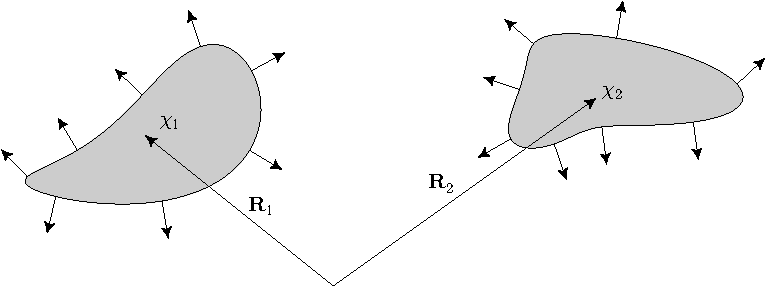
\includegraphics[width=\columnwidth]{fig/spud_sketch}
% %   \caption{Geometry for interacting dielectric bodies of susceptibility $\chi_j$, centered at
% %     $\vect{R}_j$ relative to the origin.  The surfaces mark $\sigma_j=0$, and the surface normal vectors $\hat{n}_j$
% %     are also marked.}
% %   \label{fig:spud_sketch}
% % \end{figure}

% The preceding methods offer an intuitive picture of the Casimir force,
% however they are poorly behaved as one takes the strong coupling limit.  
% For a typical path of $N$ steps pinned to the surface, approximately half 
% of the path will lie inside the body.  For $\chi\gg N$, the denominator $\langle\epsr\rangle^{-1/2}$ dominates
% the integrand, so estimate of the derivatives tends to zero as $\chi^{-1/2}$ for almost all paths.  
% Only rare paths which start on the surface, but do not enter the bulk of the body will contribute significantly.  
% As a result the estimated force goes to zero in the strong-coupling limit.
% In this section we develop an alternative expression which is better behaved in the strong-coupling
% limit and makes direct contact with prior work on Dirichlet worldlines.  


% This is exactly the construction of paths employed by Gies and Weber for computing 
% forces in the sphere-plate and cylinder-plate geometries in the Dirichlet limit~\cite{Weber2010}.  
% In that work they shift the paths so that the path just grazes the plane.  The force on the planar
% surface is computed by integrating the over the times when the path intersects the spherical or cylindrical surface.
% The expressions presented here extend their results by accounting for finite $\chi$, 
% and are framed in terms of general geometries.  

% In general, different classes of paths are important in the finite $\chi$ and strong-coupling 
% cases.  At small $\chi$, the most important path statistic is the sojourn time within the bodies,
% while in strong-coupling regime, the first-touching time is the most important statistic.    
% This is correspondence was previously used to describe the numerical convergence properties of as 
% the resolution of the paths was varied~\cite{Mackrory2016}.  
% More practically, this makes it difficult to use a single class of loops to evaluate the potential at all $\chi$:
% in weak-coupling one wants a path-ensemble that enters all of the bodies, while in strong-coupling
% it is the paths that just touch the surfaces that are most important.

% The expressions for the force in Eqs.~(\ref{eq:pinning_force}) and (\ref{eq:occupation_force})
% reflect taking two limits in different orders, namely the taking the large $N$ limit and differentiation.  
% The first derivation assumed an arbitrarily fine path where $N\gg \chi$ for all $\chi$.  Under
% differentiation the arbitrarily fine paths can be pinned to the surface, and there is a range of 
% $\cT$ where the integrand is non-zero.  However for a discrete path of length $N$, for sufficiently large $\chi$, 
% this range of $\cT$ is inaccessible, and thus the naive numerical estimate fails.    
% The second derivation instead takes the $N\rightarrow\infty$ expression last, while using well-behaved
% expressions as $\chi\rightarrow\infty$, as is better suited to a numerical method based on discrete paths.  
% This method instead highlights finding the times when the number of points inside each body 
% change.  

\subsection{Numerical Implementation of TE Casimir Forces}
\begin{align}
  \vect{F}_2 =& (-1)\frac{\hbar c N}{2(2\pi)^{D/2}}\intzinf \frac{d\cT}{\cT^{1+D/2}}
  \hspace{-2ex}\oint\limits_{\sigma_2(\vect{x}_0-\vect{R}_2)=0}  \hspace{-4ex} dS
\nonumber\\
  &\hspace{0.5cm}\times \sum_{n=0}^{N-1}\sum_{m=1}^{N-n-1}\bigdlangle\hat{n}_2(\vect{x}_0)
  \I[1]m\I[2]n f_{m,n}\bigdrangle_{\vect{x}(t)}
  \label{eq:occupation_force}
\end{align}
where the material dependence is carried by 
\begin{align}
  f_{m,n}&:=c_{m,n}-c_{m,n+1}-c_{0,n}+c_{0,n+1},\\
  c_{m,n} &:= \bigg( 1 + \frac{m\chi_1+n\chi_2}{N}\bigg)^{-\alpha},
\end{align}

\subsection{Numerical Implementation for TE Potential Curvature}

The path integral for the potential curvature in the occupation numbers apporach requires paths 
that are constrained by $\sigma_1(\vect{x}_j)$ and $\sigma_2(\vect{x}_k)$.  
There are a couple approaches to take here.  First, we could generate paths and then retroactively
find points close to the requisite surfaces, and perturb those paths such that the points do touch the 
surface.  We would then sum over all possible combinations of the indices close to the surfaces.
In this approach we would sample a position $x_0$, and then a time $\cT$.  Then we would find the 
near-intersections, and sum the integral over perturbing these.  

Recall, the potential curvature is 
\begin{align}
  C_{ij} =& \frac{\hbar c N}{2(2\pi)^{D/2}}\intzinf\frac{d\cT}{\cT^{1+D/2}}
  \hspace{-2ex}\oint\limits_{\sigma_2(\vect{x}_0-\vect{R}_2)=0}  \hspace{-4ex} dS\, \hat{n}_1(\vect{x}_0)
  \nonumber\\ 
  &\times\biggdlangle 
  \sum_{k=0}^{N-1}\hat{n}_2(\vect{x}_k)\mathcal{G}(\vect{x}_0,\vect{x}_k,k,\cT)
  \nonumber\\
  &\hspace{0.75cm} \times\sum_{n=0}^{N-2}\sum_{m=0}^{N-n-2}\I[1]n\I[2]m g_{m,n}
  \biggdrangle_{\vect{x}(t)|\sigma_2(\vect{x}_k-\vect{R}_2)=0}
\end{align}
where 
\begin{align}
  g_{m,n}=c_{m+1,n+1}+c_{m,n}-c_{m+1,n}-c_{m,n+1},
\end{align}

That effort scales quite badly roughly as an additional $N^2$.  
We could pick the a pair of fixed indices based on their probability of occuring?  
Secondly, we could also 

This integrand is non-zero for paths that touch both bodies.  In the strong-coupling limit,
only paths that just graze the bodies will contribute.  However at finite $\chi$, all paths 
are useful since paths with a finite sojourn time contribute significantly.  

This suggests a two-fold approach: generate paths constrained to touch without regard for their
occupation time (which will capture small $\chi$), and also isolate a subset of patsh which just touch the 
bodies (which will capture large $\chi$.  

We can either directly generate the paths that obey the constraints, or we can generate 
generic paths and then check whether these paths touch the desired surfaces.  

In the second strategy, the paths are generated, and we then check if there are any points
on the path which are close to a surface.  Mathematically 
$\text{min}_x|\vect{x}_j-\sigma_b(x)|\sim \sqrt{\Delta T}$.  We would then find all such points
for both bodies and then randomly select a pair to be pinned to the surface.
 We would also have to introduce the correction
for distorting this path point to lie on the surface,
\begin{equation}  
  P_{\text{pin-corr}} = \frac{P_{\text{pinned}}}{P_{\text{free}}}
  =\frac{ e^{-|\vect{x}_{j+1}-\vect{x}^*|^2/(2\Delta T)-|\vect{x}_{j-1}-\vect{x}^*|^2/(2\Delta T)  } }
  {e^{-|\vect{x}_{j+1}-\vect{x}_j|^2/(2\Delta T)-|\vect{x}_{j-1}-\vect{x}_j|^2/(2\Delta T)  }},
\end{equation}
where $x^*$ is the nearest point to the surface to $\vect{x}_j$.


\subsubsection{Direct Construction of constrained paths}

Alternatively,  we can enforce the touching constraint directly and make the paths touch the bodies by constructing
paths which are fixed at steps $j$ and $k$ to touch the surface, and sum over all $j,k\in {1,N}$.  
Evidently the direct approach will create many paths with small contributions, particular if $j-k \sim 1$.
This can be made more efficient by exploiting the Gaussian factor as a probability distribution.

In computing the energy the Gaussian is introduced for the purpose of importance sampling, and must
be factored out.  In this case, the Gaussian factor is already manifest, and should be taken into account
when sampling time.s   
We would sample times from Eq.~\ref{eq:expT}, with 
\begin{equation}
  T_0 = \frac{N^2d^2}{2\Delta(N-\Delta)} \label{eq:T0_curvature}
\end{equation}
where $\Delta$ is the difference in indices at the crossing points.
The result of using this is as our probability distribution is to factour out a normalization constant,
which leaves the integrand as 
\begin{equation}
  c=\frac{N}{\sqrt{2\pi\Delta(N-\Delta)}}\Gamma(s-1)\bigg(\frac{N^2d^2}{2\Delta(N-\Delta)}\bigg)^{-s+1}
    =\frac{2^{s-1}\Gamma(s-1)}{\sqrt{2\pi} d^{2s-2}}\bigg[\frac{\Delta(N-\Delta)}{N^2}\bigg]^{s-3/2}
\end{equation}
where the exponent $s=1+(D+1)/2=7/2$ accounts for the path integral normalization and the Gaussian factors of $T$ at
zero temperature.    
The values for the difference between the pinning indices $\Delta$ are found by numerical root-finding, using bisection.
The cumulative probability distribution for $\Delta$ is
\begin{gather}
 S_\Delta = \frac{1}{S_{N-1}}\sum_{j=1}^\Delta \bigg[\frac{j(N-j)}{N^2}\bigg]^{s-3/2}
\end{gather}
Given a uniform random number $u$, the corresponding index $\Delta$ must satisfy $S_{\Delta-1}<u<S_\Delta$.
The difference $\Delta$ can be found by bisection and starting with estimates at $S_0$ and $S_{N-1}$.
The final expression for the potential curvature is
\begin{align}
  C_{ij}%   =& \frac{\hbar c}{2(2\pi)^{D/2}}\sum_{j,\Delta>0}\int \frac{d\cT}{\cT^{1+D/2}}\biggdlangle \int d\vect{x}_0
%   \frac{N^2e^{-N^2d^2/[2 \Delta(N-\Delta)\cT]}}{\sqrt{2\pi \cT \Delta(N-\Delta)}}\nonumber\\
%   &\times
%    \hat{n}_1(\vect{x}_j)\hat{n}_2(\vect{x}_{k})
%    \sum_{n=0}^{N-2}\sum_{m=0}^{N-n-2}\I[1]n\I[2]m g_{m,n}
%    \biggdrangle_{\vect{x}(\cT);{\sigma_1(\vect{x}_j-\vect{R}_1)=0\atop \sigma_2(\vect{x}_{j+\Delta}-\vect{R}_2)=0}}\\
% =& \frac{\hbar c}{2(2\pi)^{D/2}}\sum_{j}\int d\vect{x}_0\biggdlangle 
% \frac{2^{s-1}\Gamma(s-1)S_{N-1}}{\sqrt{2\pi}|\vect{x}_j-\vect{x}_{j+\Delta}|^{2(s-1)}}
%   \hat{n}_1(\vect{x}_j)\hat{n}_2(\vect{x}_{k})
%   \sum_{n=0}^{N-2}\sum_{m=0}^{N-n-2}\I[1]n\I[2]m g_{m,n}
%   \biggdrangle_{\Delta,\cT,\vect{x}(\cT);{\sigma_1(\vect{x}_j-\vect{R}_1)=0\atop \sigma_2(\vect{x}_k-\vect{R}_2)=0}},
=& \frac{\hbar c}{2(2\pi)^{D/2}}\sum_{j}\int d\vect{x}_0\biggdlangle 
\frac{3S_{N-1}}{|\vect{x}_j-\vect{x}_{j+\Delta}|^{5}}
  \hat{n}_1(\vect{x}_j)\hat{n}_2(\vect{x}_{k})
  \sum_{n=0}^{N-2}\sum_{m=0}^{N-n-2}\I[1]n\I[2]m g_{m,n}
  \biggdrangle_{\Delta,\cT,\vect{x}(\cT);{\sigma_1(\vect{x}_j-\vect{R}_1)=0\atop \sigma_2(\vect{x}_k-\vect{R}_2)=0}},
\end{align}
where we have used $\dlangle \cdots\drangle_{y; C}$ to denote ensemble averaging over quantities 
$y$ subject to possible constraints $C$.  The first pinning positions $j$ are uniformly sampled over,
the second pinnings are sampled from $P_\Delta$ with $k=j+\Delta$, and the times are sampled from
$P_{\text{exp-T}}(T;T_0,1+(D+1)/2)$, with $T_0$ given by Eq.~(\ref{eq:T0_curvature}).  
The paths are still then constructed subject to the constraints of touching the bodies at the appropriate
indices.  The remaining integrand is evaluated for the resulting paths.  




\section{Numerical Results: Casimir-Polder Energies}

    \subsection{TE Polarization - Atom-Plane}
    \begin{enumerate}
      \item Simple Trapezoidal rule
      \item Convergence arguments
      \item ``Exact methods''
    \end{enumerate}

    \subsection{TE Polarization - Atom-Plane Gradients}

    
    \subsection{TM Polarization}

    \begin{enumerate}
      \item Need gradient estimation.  Use Malliavin calculus~\cite{Fournie1999, Chen2007,Kohatsu-Higa2003}.
        Formal introductions \cite{Nualart2006, Malliavin2006, DiNunno2009}.
      \item Birth-death methods to handle product of increments.  Related to Genealogical 
        methods used in rare-event simulation.  
      \item Histogram of raw values, with/without birth-death.
    \end{enumerate}


\section{Numerical Results: Casimir Energies}

\subsection{TE Casimir Energies - Plane-Plane}


\subsubsection{Scaling with N}


\subsection{TE Casimir Gradients - Plane-Plane}




\subsection{TM Casimir Energies - Plane-Plane}

\subsubsection{Scaling with N}


    
    % \section{Planar Dielectrics}




    % \section{Atom-Sphere}
    % \section{Atom-Cylinder}

    % \section{Plane-Sphere}

%%% Local Variables: 
%%% mode: latex
%%% TeX-master: "thesis_master"
%%% End: 

 \chapter{Electromagnetic Worldlines - General Results}

There are only general ideas at this point.
There are two options- first take the gauge-theory version.
Second treat linear coupling between the variables with rotation based on the current surface normal.



    % \section{Atom between Angled Plates}
    % \section{Plane-Sphere}
    % \section{Surface Roughness and corrugations}

%%% Local Variables: 
%%% mode: latex
%%% TeX-master: "thesis_master"
%%% End: 

 \chapter{``Realistic'' Quantum Trajectories for Position Measurements}

      \section{Position Dependent measurement operators}

      \subsection{Initial Setup}
      \begin{itemize}
        \item Atom emitting light.  Assume dipole transition.
        \item Assume atom driven by resonant probe beam, while trapped in far off-resonant
          dipole trap.  This aligns atomic dipoles in particular direction.  
        \item Atomic Hamiltonian
          \begin{equation}
            H = \frac{\vect{p}^2}{2m}+\sum\hbar \omega\sigma_z
            -\sum_i\vect{d}\cdot\vect{E}_i(\vect{x},t)
          \end{equation}
          center-of-mass motion, internal energy levels, and interaction with external fields.  
        \item Operators defined as 
          \begin{gather}
            \sigma = |g\rangle\langle e|\\
            \sigma^\dag = |e\rangle\langle g|\\
            \sigma_z = |e\rangle\langle e|-|g\rangle\langle g|
          \end{gather}
        \item Commutation relations
          \begin{gather}
            [\sigma^\dag,\sigma] 
            %= [|g\rangle \langle e|, |e\rangle \langle g|]
            = \sigma_z\\
            [\sigma, \sigma_z]   = 2\sigma\\
            [\sigma^\dag, \sigma_z]   = -2\sigma
          \end{gather}
        \item Consider spontaneous emission.  
        \item Stochastic Master Equation (approach heavily influenced by Quantum Optics notes).
          No conditioning
          \begin{equation}
            d\rho = -\frac{i}{\hbar}[H,\rho]dt + \frac{\Gamma}{2} \dec[\sigma e^{i\vect{k\cdot x}}] dt,
          \end{equation}
          where decoherence super-operator is 
          \begin{equation}
            \dec[A]\rho = 2A\rho A^\dag - A^\dag A\rho - \rho A^\dag A.
          \end{equation}
          Density matrix $\rho$ for full center of mass, and internal degrees of freedom.  
          \item Stochastic increment $df = f(t+dt)-f(t)$.
          \item For an experiment monitoring the flourescence via angle-resolved emission,
          we can model the atom's evolution via the following stochastic Master equation (SME)
          \begin{align}
            d\rho =& -\frac{i}{\hbar}[H,\rho]dt - \frac{\Gamma}{2}\hom[\sigma^\dag\sigma]\rho dt
            + \int d\Omega_k \jump[\sigma e^{i\vect{k}\cdot\vect{x}}]\rho dN_k
          \end{align}
          where homodyne and jump operators are 
          \begin{align}
            \hom[A]\rho = A\rho + \rho A^\dag - \tr[\rho(A+A^\dag)]\rho\\
            \jump[A]\rho = \frac{ A\rho A^\dag}{\tr[A\rho A^\dag]} - \rho.
          \end{align}
          The Poisson increments $dN_k$ have mean rate
          \begin{equation}
            dN_k = \Gamma\Tr[\sigma^\dag\sigma\rho] dt.
          \end{equation}
          If we account for the dipole emission pattern, assuming the atom's have their dipole preferentially
          aligned via the effective dipole potential, then 
          \begin{equation}
            dN_{k,i} = \Gamma\Tr[\sigma^\dag\sigma\rho]|u_i(\vect{k})|^2 dt.
          \end{equation}
          where $u_i(\vect{k})$ is the dipole emission pattern at wave-vector $\vect{k}$.  Normalized
          so that $\sum_{i=0,\pm}\int d\Omega_k |u_i|^2 = 1$.

          \item Inefficiency handled by introducing a loss-channel, and tracing over events in that 
          channel.  

          \item For pure-states undergoing continouus measurement , we can unravel the density matrix as an ensemble of pure states.  
          \begin{align}
            d|\psi\rangle = -\frac{i}{\hbar} H|\psi\rangle dt -\frac{\Gamma}{2}
            \left[\sigma^\dag\sigma-\langle \sigma^\dag\sigma\rangle\right]|\psi\rangle dt 
            +\bigg( \frac{\sigma e^{-i\vect{k}\cdot\vect{x}}|\psi\rangle}{\langle \sigma^\dag \sigma\rangle ^{1/2}}
            -1\bigg)dN_k,
          \end{align}
          where the Poisson process $dN_k$ has mean rate 
          \begin{equation}
            \dlangle dN_k\drangle = \Gamma \langle \sigma^\dag\sigma\rangle |u_i(\vect{k})|^2 dt
          \end{equation}
        \item Can also consider mixing signal with local oscillator.  Amplifies signal considerably.
          Different unravelling (get dipole phase information instead of excited/ground state info)

      \end{itemize}
      \subsection{Adiabatic Elimination}
      \begin{itemize}
        \item Adiabatically eliminate atoms internal state.  We assume that the 
          fluorescence occurs on a much faster time-scale than the atom's motion.  This 
          is the same logic used in developing the effective atomic-potential.  We assume that 
          there is a strong, far-off resonant field, and a weak resonant probe.  Far-off resonance
          field leads to confining potential
          \begin{equation}
            V_{\text{dipole}}(x) = \frac{\vect{\Omega}_d(\vect{x})\cdot\vect{\Omega}^*_d(\vect{x})}{\Delta}
          \end{equation}
          Formally, can find Heisenberg equations of motion, and solve in ``steady-state''.
          \begin{itemize}
            \item Input-output theory equations\cite{Gardiner1985, GardinerZoller}
              \begin{equation}
                da = -\frac{i}{\hbar}[a,H] -[a,c^\dag]\left(\frac{\gamma}{2}c + \sqrt{\gamma}b_{in}(t)\right)
                -\left(\frac{\gamma}{2}c^\dag + \sqrt{\gamma}b^\dag_{in}(t)\right)[a,c]
              \end{equation}
              where $c$ is the operator coupled to the bath, and $b_in$ in the input noise operator.  
              In rotating picture for $\sigma$
              \begin{equation}
                \dot{\sigma} = -i[\sigma,\omega\sigma_z/2+ \sigma^\dag \alpha]
                -[\sigma,\sigma^\dag]\left(\frac{\Gamma}{2}\sigma + \sqrt{\Gamma}b_{in}\right)
              \end{equation}
              Then use $[\sigma,\sigma^\dag]\sigma = -2\sigma_z\sigma = 2\sigma$
              \begin{equation}
                \dot{\sigma} = -(i\omega+\Gamma)\sigma +\sigma_z\alpha + \sigma_z\sqrt{\Gamma}b_{in}
              \end{equation}
              \comment{factors in defining Rabi frequency?}
            \item Also then need equation for $\sigma_z$
              \begin{align}
                \dot{\sigma}_z &= -i\left([\sigma_z, \sigma\alpha^*+\sigma^\dag\alpha   \right)
                -[\sigma_z,\sigma^\dag]\left(\frac{\Gamma}{2}\sigma + \sqrt{\Gamma}b_{in}\right)
                -\left(\frac{\Gamma}{2}\sigma^\dag + \sqrt{\Gamma}b^\dag_{in}\right)[\sigma_z,\sigma]\\
                &= i\left(2\sigma\alpha^*-2\sigma^\dag\alpha\right)
                +(-2)\sigma^\dag\left(\frac{\Gamma}{2}\sigma + \sqrt{\Gamma}b_{in}\right)
                -\left(\frac{\Gamma}{2}\sigma^\dag + \sqrt{\Gamma}b^\dag_{in}\right)2\sigma
              \end{align}
              Now have two coupled SDEs.  

              \begin{align}
                \dot{\sigma} &= -(i\omega+\Gamma)\sigma +\sigma_z\alpha + \sigma_z\sqrt{\Gamma}b_{in}\\
                \dot{\sigma}_z &= -\Gamma(\sigma_z+I)/2 +2i\left(\sigma\alpha^*-\sigma^\dag\alpha\right)
                -2\sqrt{\Gamma}(\sigma^\dag b_{in}  -b^\dag_{in}2\sigma)
              \end{align}
              
              Solve on average, in steady state. $\dot{f}=0$.
              \begin{align}
                \sigma = \frac{\alpha}{i\omega + \Gamma}
              \end{align}
              

          \end{itemize}
          

          More justified approach, to integrate equations of motion, and solve approximately
          Then find effective Hamiltonian that reproduces those effective equations of motion.
          \begin{equation}
            \sigma\rightarrow \frac{|\vect{\Omega}|}{\Gamma}.
          \end{equation}


      \end{itemize}
      \subsection{Effective Position Measurement}
      \begin{itemize}
        \item No-conditioning
          \begin{equation}
            d\rho_{CM} = -i[H_{\text{eff}},\rho_{CM}]dt + \Gamma \int d\Omega_k\dec[|\vect{\Omega} e^{i\vect{k\cdot x}}] dt
          \end{equation}
        \item Measurement operators are transformed copies of electric field emitted by atoms.
          That is combination of atomic dipole pattern, with spatially dependent emission rate.
          Electric field emitted by atoms is
          \begin{equation}
            \mu = e^{i\vect{k}\cdot\vect{x}}E(\vect{x})
          \end{equation}
          Transform electric field via propagation and lens system.  Electric field incident 
          on detector is a linear superposition of emitted fields.  Then apply transformation
          function on that linear sum.  That is the field at the detector.  
        \item Note, for resonance fluorescence, one integrates over all emission directions for 
          full set of emission operators at each position.  
          Consider lens system as a linear map on electric fields.  
          \begin{equation}
            \mu(x) = \int d\Omega_k\,e^{i\vect{k}\cdot\vect{x}}u_i(\vect{k})\alpha(\vect{x})
          \end{equation}
          


      \end{itemize}



      \section{Zeno Effect and Strong Measurements}

      \begin{itemize}
        \item Include figures/simulations showing reflection
        \item Discuss physics of two decay channels: reflection from re-emission into beams, inference from 
          detectin emitted photons.
        \item Similarity to stochastic potential.  
        \item No net force.  Probability of reflection might approach one, but effect on 
          state is larger, so $d\langle p\rangle = 0$
        \item Cite work commenting on our work.  Moving beyond purely perturbative approach.  
        \item Figure: Reflection as function of $\chi$
      \end{itemize}

      \section{Trajectories for EMCCD cameras}

      \begin{itemize}
        \item Handle noise, uncertainty by building model for measurement process
          including all relevant noise, loss mechanisms.  Build a full, pure 
          trajectory picture including random processes.
          Then average over unobservable processes.   Weight each trajectory
          with Bayesian statistics (re picture of evolution of quantum state). 
        \item Warzsawski and Wiseman modelling 2-level atom emitting light onto 
          APD.  Include dark counts, down-time, finite collection efficiency.
      \end{itemize}
      

      \subsection{EMCCD Amplification and Noise Processes}

      \begin{itemize}
        \item Review of useful concepts from Jeremy Thorne's thesis.  
        \item Camera adds clock-induced charge at given Poissonian rate.
        \item Amplification process exponentially stretches out $n$ photons.
        \item Then Gaussian read-out noise.  
      \end{itemize}

      \begin{itemize}
          \item In order to build quantum trajectories based on this, exploit Bayesian statistics
          to weight all trajectories.  
          \begin{equation}
            |\psi\rangle = \sum_{\text{traj}} P(\text{traj}|\text{outcome})|\psi_{\text{traj}}\rangle.
          \end{equation}
          Find the weighting probability via Bayesian statistics
          \begin{equation}
            P(A|B) = \frac{P(B|A)P(A)}{\sum_AP(B|A)P(A)}
          \end{equation}
          \item Furthermore, must trace over unobserved quantities, such as clock-induced 
          charge, spontaneous emission into free-space.  
      \end{itemize}

      

%%% Local Variables: 
%%% mode: latex
%%% TeX-master: "thesis_master"
%%% End: 

 \chapter{Conclusion}

The goal of this thesis was to develop a general purpose numerical method
employing the worldline method to calculate electromagnetic Casimir energies. 
We have been partially successful in those aims.   

Following~\citet{Bordag1998,Bordag1999}, we developed a full vector path integral~(\ref{eq:vector_path_integral}) for
the EM field.  So far it has not be implemented as a numerical method.
Instead, we developed an approximate worldline description for the EM field in terms of two independent scalar fields, corresponding 
to the TE and TM polarizations.   
Although the decoupled scalars are adapted to a planar geometry, 
they share some similarities with the potentials in the full vector
path integral, and are a useful test case in their own right.  

We showed analytically and numerically that the polarization worldline path integrals recover the known expressions for the 
Casimir--Polder and Casimir energies in planar geometries, at zero and high temperature.  
Doing so involved regularizing singular TM potentials, and finding analytical solutions to the path integral
in certain geometries.  The analytical expressions for the path average of the TM potential are 
 essential for numerical computations with this method.  

Even with regularized solutions, it was necessary to develop techniques to efficiently
sample the worldline path integral.  The TE integrand was relatively simple to evaluate, while the TM
integrand is much more challenging and still under study.
The birth-death method for sampling paths was essential for bringing the statistical errors under control, 
and the partial averaging method also allowed us to evaluate the derivatives required for the TM method.
The numerical methods we developed are in agreement with the expected analytical results.
% where previously, the finite difference method had been previously plagued by convergence issues.

The methods that were developed could be used as an (uncontrolled) approximation to the Casimir effect in a general geometry.
They will also probably be useful in handling the vector path integral.    
In cases where path integrals can be analytically solved for open Brownian bridges [such as
Dirichlet~(\ref{eq:Dirichlet}) and TM boundary conditions~(\ref{eq:TM_potential})], 
those expressions can be applied locally at each step of the path.  
At each step, the potential could be computed using a local planar approximation to the exact solution.
The local solutions joined together along the path, could form a basis for solving a path integral
in general, based on the local approximations throughout the path.  

Another possible approach to leveraging the results contained here into a general method is to consider 
how the two scalar polarizations are coupled.  
At each point along the path, the EM field could be split into the TE and TM polarizations based 
on the nearest surface normal.
The weights for the polarizations are the components of an auxiliary two component vector that travels along the path.
At each step, the terms acquire the appropriate TE or TM potential, 
and are then coupled together via a rotation matrix where the rotation
angle depends on the change in the surface normal.  

% In the introduction we noted that the scattering method is currently the only general
% method for computing EM Casimir energies in arbitrary geometries, and that is still true.  
The worldline method has not yet been generalized to full electromagnetism.   
%The work presented here brings that prospect closer.  
However, the worldline has a number of attractive features such as its simple parallelism, and the possibility
for superior performance in very complicated geometries.  Given the progress thus far,  
I believe that this method is worth developing further, where it could complement existing methods
and may have uses in electromagnetism beyond just Casimir physics.




%%% Local Variables: 
%%% mode: latex
%%% TeX-master: "thesis_master"
%%% End: 

\appendix
% \chapter{Literature Review}

This is a collection of notes summarizing important papers.  I will give a condensed version of this in the introduction.  

\section{Casimir Books}

Goal: List and reference important equations/chapters.  
I need to figure out the appropriate way to cite chapters/equations/pages within a thesis.  

\subsection{Milonni: Quantum Vacuum}

Milonni~\cite{Milonnibook1994}

\subsection{Milton: Casimir Effect}
Milton~\cite{Miltonbook2001}

\subsection{Bordag}
Bordag~\cite{Bordagbook2009}

\subsection{Dalvit: Casimir Effect}
Dalvit~\cite{Dalvitbook2011}

\subsection{Parsegian: van der Waals forces}

Parsegian~\cite{Parsegian2006}



\subsection{Israelachivili:Molecular Forces}

Israelachivili~\cite{Israelachvili2011}


\section{Field Theory Books}

\subsection{Brown Quantum Field Theory}

\cite{Brown1994}
Path integrals and stat mech

Field theory.  

Field theory Renormalization

\subsection{Peskin and Schroeder}
\cite{Peskin1995}

\subsection{Srednicki: Quantum Field Theory}
\cite{Srednicki2008}

\subsection{Altland and Simons: Condensed Matter Field Theory}
\cite{Altland2011}

Linear Response

Effective theory

\subsection{Abrikosov:Condensed matter field theory}

\cite{Abrikosov1975}
Thermal field theory

Feynman-Diagram approach to Casimir.


\section{Stochastic Books}

\subsection{Oksendahl}

\subsection{Durrett}

\subsection{Gardiner}



\section{Early Papers}

\subsection{Casimir48}


\cite{Casimir1948}

\subsection{CasimirPolder1948}


~\cite{CasimirPolder1948}.  

\subsection{Lifshitz1956}

~\cite{Lifshitz1956}.  

\subsection{Dzyaloshinkii1959}

\cite{Dzyaloshinskii1959}
\subsection{Dzyaloshinksii1961}

\cite{Dzyaloshinskii1961}

\subsection{Mclachlan1963}

\cite{Mclachlan1963}

\section{Experimental Papers:Casimir}

\subsection{Lamoreaux1997}

\cite{Lamoreaux1997}
\subsection{Sushkov2011}

\cite{Sushkov2011}
\subsection{Mohideen1998}
\cite{Mohideen1998} 

\subsection{Chan2001}

\cite{Chan2001}
\subsection{Bressi2002}

\cite{Bressi2002}

\section{Experimental Papers:Casimir-Polder}
\subsection{Harber2005: Cornell BEC}

\cite{Harber2005}
\subsection{Obrecht2007:Cornell BEC}
\cite{Obrecht2007}

\subsection{Antezza chapter}
\cite{Dalvitbook2011}

\subsection{Alton2011:Atoms-Toroid}

\cite{Alton2011}. 

\subsection{Hung2013:Atom-Microcavity}
 Atoms above 1D Microcavity \cite{Hung2013}


\subsection{Atom-Chips:Folman2000}

\subsection{Atom-Chips:Schneider2003}

\cite{Folman2000,Schneider2003}

\subsection{Cronin-Beams}

\cite{Perreault2005,Lonij2009}

\subsection{Sukenik:Atoms through Cavity}

\cite{Sukenik1993}

\subsection{Experimental arguments}

\begin{itemize}
\item Controversies about role of zero temperature pole.  
\item Lamoreaux favors Drude model, Capasso favours plasma model.
\item Seems experiments favour more 
\end{itemize}

\subsection{Geckos: Autumn2002}
\cite{Autumn2002}

\cite{Hawkes2014}

\subsection{Modifications to gravity}

\begin{itemize}
\item Modifications to gravity on $1\mu m$ or $1mm$ scale.  Cite Lamoreaux 2000 Paper.  Gervaci?
Yukawa type forces.  
\item Subtract off Casimir force background.  Tino group.  Use Casimir shield with fairly thick gold to have same Casimir force, and then vary the medium behind it.  Longer range gravity should lead to Requires very careful measurements, on top of carefully extracting Casimir force.   
\end{itemize}

\subsection{Papers: Proximity Force Approximation}

\begin{itemize}
\item Find first use?  Lamoreaux mentions usage.  Derjaguin?\cite{Derjaguin1956} \cite{Blocki1977}
\item Note problem with non-additivity. 
\item Good as order of magnitude estimate?  Useful if very limited curvature, or effectively approximate geometry as planar.  
\end{itemize}

\subsection{Schwinger: Green function methods 1978}

\cite{Schwinger1978, Milton1978}

Scalar green function methods.  Milton book.  
Planes

\subsection{Milton1978}
Spheres

\begin{itemize}
\item Green tensor methods
\item Cite Barton
\item Cite Philbin(?)
\item Cite Vogel and Welsch
\end{itemize}

\section{Papers: Theory- Reflection Matrix}

\subsection{Balian and Duplantier}
\cite{Balian1977} \cite{Balian1978}
\subsection{Lambrecht/MaiaNeto}

\cite{Lambrecht2006}
\cite{MaiaNeto2008}
\cite{Canaguier-Durand2012}

\subsection{Scattering Matrix Path Integral Methods}

\subsection{Stratton}
Surface integral equations (Stratton-chu)
\cite{Stratton1941}

\subsection{Emig/Buscher}

Paper on deformations showing you can use homogenous green functions within bounding surface.  

\subsection{Emig/Rahi}

Multipole expansion
\cite{Buscher2004}
\cite{Emig2004, Emig2007, Rahi2009}

\subsection{Kenneth/Klich}
\cite{Kenneth2006}
\cite{Kenneth2008}

\subsection{Reid/Johnson/Rodriguez}

Early numerical papers.
\cite{Rodriguez2007},\cite{Rodriguez2007a}, \cite{Rodriguez2009}.  Note use of existent analytical methods and similarities to existent numerical FTDT techniques Builds on earlier papers (uses better basis) 

Cite Johnson textbook.\cite{Johnson2011}

\subsection{Reid papers}

\cite{Reid2009},\cite{Reid2011}, \cite{Reid2013} 
Note success, applicability.  \comment{Cite experimental tylenol pill paper}

\section{Repulsion}

\begin{itemize}
\item Cite Milton paper on anisotropy \cite{Milton2012, Milton2012a}
\item Cite work on metamaterials (hydrogen mirror)
\item Cite Milonni/rosa showing broad-band \cite{Rosa2010}
\end{itemize}

\section{Papers: Worldlines}

Note citations in bordag/johnson mostly as dismissive and limited  

\subsection{Effective actions}

\cite{McKeon1993, Strassler1992,Schubert2001}

\comment{Other references - was one contemporaneous with Strassler? Bern-Kosower}

\comment{Cite 1950 Feynman Scalar QED section}

\cite{Schubert2001}.  

\subsubsection{Applied to QED}

For example, the worldline method has been used to compute relativistic field effects for QED such as the Lamb shift~\cite{Schmidt1995}.  It has also been used as a numerical algorithm\cite{Mazur2014}.

\subsection{Feynman Path Integral for QM}

\cite{Feynman1948,Feynman1965,Brown2005}.

\subsection{Papers: Gies Worldline}

\subsubsection{Gies 2003}
\cite{Gies2003}

\begin{itemize}
\item Cite earlier paper by themselves for first worldline numerics?   Found citations for PFA.
\item Action for scalar fields.   Massive scalar field interacting with some potential $V(x)$.  $V$ has dimensions of mass-squared.  (Field theory units $\hbar=c=1$, so $E=mc^2$)
\begin{equation}
\cL = \frac{1}{2}\partial_\mu\phi\partial^\mu\phi +\frac{1}{2}m^2\phi^2+\frac{1}{2}V(x)\phi^2
\end{equation}
\item Complete unrenormalized quantum effective action for $V$ (integrate out fields $\phi$) is 
\begin{align}
  \Gamma[V] &=\frac{1}{2}\tr\ln \left[ \frac{-\partial_\mu\partial^\mu +m^2 + V(x)}{-\partial_\mu\partial^\mu +m^2}\right]\\
&   =-\frac{1}{2}\int \frac{d\cT}{\cT} \int d^D x \left\{ \langle x|e^{-\cT[-\partial_\mu\partial^\mu +m^2 + V(x)]}|x\rangle -\frac{e^{-m^2 \cT}}{(4\pi \cT)^{D/2}}\right\}
\end{align}
Working in $D=d+1$ euclidean space-time dimensions.  
\item Convert matrix element to path integral.  
\begin{equation}
  \int d^D x \langle x|e^{-\cT[-\partial^2+V(x)]}|x\rangle = \int d^D x_{\text{CM}} \mathcal{N}\int_{x(0)=x(\cT)}Dx e^{-\int_0^\cT d\tau \dot{x}^2/4}
\end{equation}
Comments: Fix normalization from limit of zero potential (which is evaluated in momentum basis), and note that choice to drop factors of 2 has left them with an extra $\sqrt{2}$ in the definition  of the loops.
\begin{align}
\langle x| e^{\partial^2T}|x\rangle &= \int d^Dp\frac{1}{(2\pi)^{D/2}} e^{-p^2T}\langle x|p\rangle\langle p|x\rangle\\
&= \frac{1}{(4\pi \cT)^{D/2}}\\
&=\cN \int_{x(0)=x(\cT)}Dx \exp\left\{-\int_0^\cT d\tau \left[\frac{\dot{x}^2}{4}+V(x_{\text{CM}}+x(\tau)\right]\right\}
\end{align}
\item Now interpret path integral as Gaussian integral/ensemble average over closed loops.  
\begin{equation}
\cN \int_{x(0)=x(\cT)}Dx \exp\left\{-\int_0^\cT d\tau \left[\frac{\dot{x}^2}{4}+V(x_{\text{CM}}+x(\tau)\right]\right\} = \frac{1}{(4\pi \cT)^{D/2}}\dlangle e^{-\int_0^\cT d\tau V[x_{\text{CM}}+x(\tau)]}\drangle
\end{equation}
Also use scaled loops: 
\begin{equation}
x_\mu(\cT t) = \sqrt{\cT}y_\mu(t),
\end{equation}
where $t\in [0,1]$, and we view $\cT$ as a parameter.  
\item Plugging in path representation
\begin{align}
\Gamma[V]=&-\frac{1}{2 (4\pi)^{D/2}}\int_{1/\Lambda^2}^\infty \frac{d\cT}{\cT^{1+D/2}} e^{-m^2\cT}\int d^Dx_{\text{CM}} \\
&\times\dlangle e^{-\cT\int_0^1dt V[x_\text{CM} +\sqrt{\cT}y(t)]}-1 \drangle
\end{align}
For time independent backgrounds use $\int dx_0 = L_{x_0}$ as ``length'' in time direction.  \comment{For partition function version Get $\beta\hbar c$ instead.}
\item \textbf{Renormalization}
Consider field theoretic renormalization (I think whereby an analogue of the Integral Trajectory Matching formalism fixes the unknown(divergent) values at some known scale - typically from a low energy experiment).  
\item Heat Kernel Expansion \comment{Cite Gilkey} .  Expand to non-diverging order to regularize UV divergences.  Each power of $V$ amounts to an external leg.  Get a Tadpole $T^{-D/2}\int dx_0 V$, and 
\item Ignore self-energies and focus on interaction energies (which are insentitive to Field theoretic divergence)
\begin{equation}
E_\text{int}= E_{V_1+V_2+\cdots}- E_{V_1} - E_{V_2}-\cdots
\end{equation}
Can carry out renormalization at loop level and thus avoid divergent sums.  
\item They note that this emphasis on interaction energy is \emph{not} a renormalization procedure.  It circumvents that for multiple bodies.  However for isolated bodies (sphere self-stress), one must specify all of the renormalization conditions, and your answers may depend on the procedure used.
\item \textbf{Numerics}
Introduce some methods (most of which are useless).
Important method is the v-loop.  An exact diagonalization of the Gaussians, under the loop closure constraint.  Note that they choose their loop constraint to be $\int d\tau y_\mu(\tau) =0$.  This amounts to making the center of mass of the loop centered on $x_\text{CM}$.  In contrast, our work has typically used $x(0)=x(\cT)=0$.  

The ``v-loop'' algorithm amounts to considering the probability measure,
\begin{equation}
P(\{x_k\}) =  \delta(x_N-x_0)\prod_{j=0}^{N}e^{-\frac{(x_{j+1}-x_j)^2}{2\Delta T}},
\end{equation}
and completing the square in the exponents to decouple the Gaussians.  
Note their version uses $\sum_{j}x_j=0$ to fix $y_N$.  
The Jacobian can be shown to unity, since the matrix is upper diagonal, with unit diagonal.  
\item \textbf{Tests}
\item Compare to parallel plate energy to get convergence. 
\item Give some consideration to finite $\lambda$ in potential.  
\begin{equation}
V(x) = \lambda\int_{\Sigma}d\sigma \delta(x-x\sigma)
\end{equation}
where $\Sigma$ is a $d-1$ dimensional surface, $\sigma$ is a reparameterization invariant measure and $x_\sigma$ points to the surface.  
\item For interaction energies, need $(e^{-V_{1+2}} - 1) -  (e^{-V_1}-1) - (e^{-V_{2}}-1)$.  If only touch one surface (of disconnected bodies) then 
no contribution, since $V_{1+2}=V_1$
\item Then consider massless scalar between sphere/plate and cylinder plate.  
\item Consider breakdown of PFA as function of separation $a$ to sphere radius $R$.  
\item \textbf{Conclusions}
\item Needs no underlying symmetry.  Precision hinges on loop parameters chosen (and presumably discretization of surfaces)
\item Claim their delta potentials are ``hard''.
\item Note finite temperature and roughness required.  
\item Note numerical differentiation to get force is hard, but derivative can be done right off the bat.  (And energy-momentum tensors)
\item Cite Feinberg and Sucher for possible path for EM quantization.  
\end{itemize}

\subsubsection{Gies2001}
\cite{Gies2001}

Use worldlines to compute EM effective action in specified background EM field, modelling interaction with scalar particle.  

\subsubsection{Gies 2006}
\cite{Gies2006}

Very similar?  Advances?  
D-loops?  Note similarity to methods of generating brownian walks by doubling intermediate points to imrpvoe resolution where required.  

\subsubsection{Gies 2006 a}
\cite{Gies2006a}

\subsection{Papers: Thermal worldlines}

\subsubsection{Geothermal2008:Klingm\"uller}
~\cite{Klingmueller2008}.  
\subsubsection{Weber2009:Inclined planes}
~\cite{Weber2009}
\subsubsection{Weber2009:Interplay}
~\cite{Weber2010}
\subsubsection{Weber2009:Spheres}
\cite{Weber2010a}.  

\subsubsection{Schaden:Pistons}

Cite Schaden applying to pistons\cite{Schaden2009}

Why?  What for?  Benefits?

\subsection{Nearby attempts}

\cite{Aehlig2011}

\cite{Maggs2006, Pasquali2008}

\section{Papers:Stochastic Methods}

\subsection{Gradients}

\subsection{Feynman-Kac}

\subsubsection{Hooghiemstra}



\section{Papers:Dielectric Quantization}



\subsection{Vogel and Welsch}


%\cite{Dung1998}
\cite{Raabe2006}
\cite{Raabe2007}

\subsection{Huttner/Barnett}

\cite{Glauber1991}

\cite{Huttner1992}

\cite{Matloob1995}
\cite{Matloob1996}


\subsection{Philbin}

\cite{Philbin2010}
\cite{Philbin2011}

\cite{Drummond2014}

\subsection{Bordag}
\cite{Bordag1998} \cite{Bordag1999}

\subsection{Bechler}

\cite{Bechler1999}
\cite{Bechler2006}




\section{Quantum Trajectories}

\subsection{Carmichael}
Cite Carmichael Rice JOSA paper.

Cite Carmichael 1993 lectures. \cite{Carmichael1993}

\subsection{Others}

Cite Marte
Cite Parkins  
Cite Gardiner \cite{Gardiner1992}
Cite Marte, Zoller, Parkins, Gardiner (MCWF) \cite{Dalibard1992}
\cite{Dum1992}

\subsection{Path integral version}


\subsection{Measuring atom positions}

 Cite Holland, Meystre.  Applied to position measurements of atoms by detecting photons.  Detection of photons localizes atoms.  
\cite{Holland1996}


\subsection{Control theory}
 Control Theory.  Cite Wiseman book.   \cite{WisemanMilburn2010}
 
Cite Steck feedback control paper.  \cite{Steck2004, Steck2006}

\subsection{Quantum chaos}

Cite Bhattacharya quantum paper.  \cite{Bhattacharya2005}

\subsection{Noisy measurements}
Cite Warshawski/Wiseman \cite{Warszawski2003}

Cite Jeremy Thorne.  


%%% Local Variables: 
%%% mode: latex
%%% TeX-master: "thesis_master"
%%% End: 

% \chapter{Code}

Details about code implementation?

%%% Local Variables: 
%%% mode: latex
%%% TeX-master: "thesis_master"
%%% End: 

 \chapter{Detailed Calculations}
\label{app:nasty_calc}
This Appendix collects a number of lengthy, but tedious calculations required in the main text.  

\section{Path Integrals in Curved Space}

In this section we will show that the potential $\VTE$ naturally emerges if we
work in a curved space.  
The problem of computing the path integral for a 
particle in curved space was first considered by deWitt~\cite{deWitt1957}.  
In a curved space, the position and momentum  operators take on slightly 
different forms reflecting the differing inner product.  
Let us follow Pauli to see one way towards handling this~\cite{Pauli1958}.  

Let us consider a curved space, with generalized coordinates $q_i$.  The metric
tensor $g_{ij}$ then gives the notion of distance, $ds^2 = g_{ij}dq^idq^j$.  
In a curved space, the volume element is $\sqrt{|g|}\prod_idq_i$, where $g=\det(g_{ij})$.   

The identity on the coordinates is 
\begin{equation}
 I_q := \int d\vect{q}\sqrt{|g|} |\vect{q}\rangle\langle {q}|
\end{equation}
This implies that the wavefunction overlap for two states $|\phi\rangle,|\psi\rangle$
is 
\begin{equation}
\langle \phi|\psi\rangle = \int d\vect{q}\sqrt{|g|} \phi^*(\vect{q})\psi(\vect{q}).
\end{equation}
In order for the identity to be idempotent ($I_q^2 = I_q$), this requires that
the overlap between coordinate eigenstates is 
\begin{equation}
\langle \vect{q}|\vect{q'}\rangle = \frac{1}{\sqrt{|g|}}\delta(\vect{q}-\vect{q}')
\end{equation}

The position and momentum operators should be hermitian, and obey the 
canonical commutation relations, 
\begin{equation}
[\op{q}_i,\op{p}_j]=i\hbar\delta_{ij}.
\end{equation}
If we define the position operators such that 
\begin{equation}
\langle \vect{q'}|\op{q}|\psi\rangle=\vect{q'}\langle \vect{q'}|\psi\rangle,
\end{equation}
then we can infer from the commutation relations, and the hermiticity condition
that the momentum operators are given by
\begin{align}
\langle\phi|\op{p}_i|\psi\rangle = \int d\vect{q}\sqrt{|g|}\phi^*(\vect{q})
\frac{1}{\sqrt{|g|}}\frac{\partial}{\partial q_i}\sqrt{|g|}\psi(\vect{q}).  
\end{align}
The presence of the extra factors of $\sqrt{|g|}$ ensures that the 
$\langle\phi|(\op{p}_i|\psi\rangle = (\langle \phi|\op{p}_i^\dag)|\psi\rangle$,
which follows from the integral represenation via an integration by parts.  

An alternative method of setting up the path integral in curved space is to 
transform that flat-space path integral to curvilinear coordinates~\cite{Gervais1976,Girotti1983}.  
The main concern in this approach is to consistently work to $\order(\Delta T)$.  
Given the typical Gaussian path measure, which implies $\Delta x^2 \sim \Delta T$, 
this requires us to also Taylor expand up to fourth order in spatial 
functions~\cite{McLaughlin1971}.    

Let us consider the following action
\begin{equation}
  S = \frac{m}{2}g_{ij}(\vect{q})\dot{q}_i\dot{q}_j - V(x)
\end{equation}
We will find the 
\begin{enumerate}
\item Lagrangian.
\item Momentum
\item Hamiltonian.  Note $pgp$ structure.  Operator ordering problem in curved space.  
  Have classical equations, with ambiguous ordering (and tiny, tiny consequences)
  for different choices.  
\item Wave equation is Laplace-Beltrami operator (what you get from changing coords
  -motivates Gervais approach.  
\item DeWitt: Path integral is kernel of appropriate Schrodinger equation.
\item Kleinert, transformation useful in curvilinear coordinates. (path integral
  for hydrogen atom.
\end{enumerate}



% \section{Path Integral in Curved Space}

% \begin{enumerate}
%   \item Path integral construction on metric-affine space is surprisingly complicated 
%     and error-fraught.  
%   \item Care is required in construction to get all terms.  
%   \item Similar to multiplicative noise in SDE.
% \end{enumerate}

% \begin{enumerate}
%   \item Given analogy of a medium to a curved space. Cite Leonhardt, Gordon  
%   \item Note general requirement for $\mu=\epsilon$.  Hard to achieve, especially broadband.
%   \item Application to TM path integral with rescaling $\epsilon$.
% \end{enumerate}

% \subsection{Operators in Curved Space}

% \begin{enumerate}
%   \item Quote Position Operator and inner product for spatial wavefunctions.
%   \item Note only momentum operator consistent with that.
%   \item Develop path integral
%   \item Show it obeys the Schrodinger equation (Grosche's test)
% \end{enumerate}

% \subsection{Transformation}

% \begin{enumerate}
%   \item Start with flat-space path integral.\cite{Gervais1976, Kleinert2012}
%   \item Introduce coordinate transformation
%   \item Choose expansion point, expand consistently to $\order(\Delta T)$.
%   \item Note connection to choice of stochastic calculus.
%   \item Expand Jacobian factors
%   \item Expand Gaussian factors
%   \item Convert to terms involving curvature tensors.
%   \item Simplify down to $1D$
%   \item Note typically small value of quantum correction.  $\hbar^2$.
% \end{enumerate}


% \section{Operator Quantization in Curved Space}

% This follows from Bryce DeWitt's early papers \footnote{
% DeWitt, B. S. \textit{Point Transformations in Quantum Mechanics}, 
% {Phys. Rev.}, \textbf{85}, 653, 1952.\\
% deWitt, B. S. \textit{Dynamical Theory in Curved Spaces I: A Review of the 
% Classical and Quantum Action Principles}, {Rev. Mod. Phys.}, \textbf{29}, 377,(1957). } .
% See also a review by Pauli\footnote{
% Pauli, W., \textit{General Principles of Quantum Mechanics}, (1980), 
% translated by P. Achuthan and K Venkatesan} 

% There are two ways of deriving the path integral in curved space.  In the first 
% formulation, we derive the relevant path integral in curved space
% by starting with the curved space Hamiltonian and quantized appropriately.  
% This requires changing the form of the momentum operators, which gain corrections.
% This is in contrast to the second approach, which starts with a flat-space path
%  integral, and transforms that path integral to curvilinear coordinates.
%  We will use $x$ to denote the curvilinear coordinates, and $q_i$ to denote the flat-space coordinates.  

% Consider the following particle Lagrangian,
% \begin{equation}
% L = \frac{1}{2}g_{ij}(x)\dot{x}^i\dot{x}^j
% \end{equation}
% with line element, $ds^2 = g_{ij} dx^i dx^j$, and volume element, 
% $dV = \sqrt{|\det[g_{ij}]|}\prod_idx_i$.  

% This has canonical momenta 
% \begin{equation}
% p_i := \frac{\partial L}{\partial \dot{x}^i} = g_{ij}\dot{x}^j.
% \end{equation}

% The equivalent Hamiltonian is 
% \begin{align}
% H & = p_i\dot{x}^i - L \\
% & = \frac{1}{2} p_i g^{-1}_{ij}p_j = \frac{1}{2}p_i g^{ij}p_j,
% \end{align}
% where  ${g^{-1}}_{ij} = g^{ij}$ is the inverse metric.  

% The choice of where to place the metric (which is a function of position)
%  relative to the momentum operators is sometimes called the 
% \textit{operator-ordering problem}.  We have no classical reason for picking
% any one of the myriad quantum operator ordering choices.  
% We will see that this operator ordering is related to our choice of stochastic calculus.  

% \subsection{Quantization}

% When we quantize this we require that the position and momentum obey the usual commutation relations
% \begin{equation}
% [x_i,p_j] = i\hbar\delta_{ij}.
% \end{equation}
% The other piece we need is representation of the identity for states.
%  We will represent the spatial and momentum identity operators as 
% \begin{gather}
% \int d\vect{x} \sqrt{g} |\vect{x}\rangle \langle \vect{x}| = 1\\
% \int \frac{d\vect{p}}{(2\pi\hbar)^d} |\vect{p}\rangle \langle \vect{p}| = 1
% \end{gather}
% This representation of the spatial identity implies the inner product between
% is
% \begin{equation}
% \langle \phi |\psi\rangle = \int d\vect{x} \sqrt{g} \phi^*(x)\psi(x),
% \end{equation}
% where we have introduced the shorthand notation, $g = \det[g_{ij}]$.
% The position space representation of the momentum operator can be de derived 
% by seeking consistency with the commutation relations and ensuring that the 
% momentum is a hermitian operator
% \begin{equation}
% \langle x| \op{p}_i|\psi\rangle = -i \frac{1}{g^{1/4}} \partial_i\left[ g^{1/4}\psi(x)\right] 
% = -i\left(\partial_i +\frac{1}{4}\frac{\partial_i g}{g}\right)\psi(x).
% \end{equation}
% We can check the hermiticity by requiring 
% $\langle\phi |\op{p}|\psi\rangle = \langle \psi |\op{p}\phi\rangle^{*}$.
%   In position space this becomes 
% \begin{align}
% \langle \phi|\op{p}|\psi\rangle & = -i\int dx\,\sqrt{g}\phi^*(x) 
% \frac{1}{g^{1/4}} \partial_x\left[ g^{1/4}\psi(x)\right]\\
% & = i\int dx\,\partial_i\left[g^{1/4}\phi^*(x)\right] g^{1/4}\psi(x)\\
% & = i\int dx\,\sqrt{g}\psi(x) \frac{1}{g^{1/4}}\partial_i\left[g^{1/4}\phi^*(x)\right]\\
% & = \langle \psi |\op{p}|\phi\rangle^*
% \end{align}
% The spatial representation of the momentum operator can also be written
% in terms of the Christoffel symbols,
% \begin{equation}
%  \frac{1}{g^{1/4}}\partial_i g^{1/4} f = \partial_i f + \frac{1}{4}\partial_i\ln(g)f.
% \end{equation}
% The Christoffel symbols are defined as
% \begin{equation}
% \Gamma_{ij}^k = \frac{1}{2}g^{kl}\left(\partial_ig_{jl}+\partial_jg_{li} 
%   - \partial_lg_{ij}\right)
% \end{equation}
% We can trace over the Christoffel symbols, 
% \begin{align}
% \Gamma_{i} &= \Gamma_{ik}^k=\frac{1}{2}g^{kl}\left(\partial_ig_{kl}+\partial_kg_{li} 
%   - \partial_lg_{ik}\right)\\
% %&=\frac{1}{2}\left(g^{kl}\partial_ig_{kl}+\partial^lg_{li} 
% %  - \partial_kg_{ik}\right)\\
% &=\frac{1}{2}g^{kl}\partial_ig_{kl} = \frac{1}{2}{g^{-1}}_{kl}\partial_ig_{kl}
% \end{align}
% This can be rewritten using $\tr-\log(A) = \log\det(A)$.  Our expression
% for the derivative involves,
% \begin{equation}
% \partial_i\log\det(g)=\partial_i\tr\log(A)=\tr\partial_i\log(A) = \tr[g^{-1}\partial_ig]
% \end{equation}
% We can then write the derivative operator as 
% \begin{equation}
% \langle \vect{q}|p_i|\psi\rangle 
% = -i\hbar\left(\partial_i +\frac{1}{2}\Gamma_i\right)\psi(\vect{q})
% \end{equation}

% This is not quite the full covariant derivative one might anticipate,
% \begin{equation}
% \nabla_iV^j = \partial_iV^j + \Gamma_{ik}^jV^k
% \end{equation}
% However, the wavefunction is a scalar, rather than a vector, and thus
% we are not tracking how the vector components are changed in a curved space. 
% Perhaps this would emerge naturally for spinors (or spin-1 particles - say for
% the photon?), where the wavefunction should be decomposed in terms of irreducible
% represenations of whatever group we are working with?

% We also need to specify the form of the matrix elements.  The matrix elements
% are:
% \begin{gather}
% \langle \vect{q}|\vect{q'}\rangle = \frac{1}{\sqrt{g}}\delta(\vect{q}-\vect{q'})\\
% \langle \vect{p}|\vect{p'}\rangle = \delta(\vect{p}-\vect{p'})\\
% \langle \vect{q}|\vect{p}\rangle = \frac{e^{ip_iq^i/\hbar}}{\sqrt{2\pi\hbar }g^{1/4}}.
% \end{gather}
% The first two relations ensure that $I_x^2=I_x$, $I_p^2=I_p$ by returning delta-functions
% with appropriate factors of the matrix.  
% The third ensures the overlap integral is independent of the basis used.  


% If we assume we have quantum Hamiltonian,
% \begin{equation}
% H = \frac{1}{2}\op{p}_ig^{ij}(\op{q})\op{p}_j
% \end{equation}
% then in position space, the Schrodinger equation is 
% \begin{equation}
% i\hbar \partial_t\psi = 
% -\frac{\hbar^2}{2}\frac{1}{g^{1/4}}\partial_i g^{1/4}g^{ij}g^{1/4}\partial_j \frac{1}{g^{1/4}}\psi(q)
%  = -\frac{\hbar^2}{2}\Delta_{\text{LB}}\psi
% \end{equation}
% This can be reordered into the form of the Laplace-Beltrami operator\footnote{
% Kleinert, H. G. \textit{Path Integrals in Quantum Mechanics, Statistics, 
% Polymer Physics and Financial Markets}, $5^{\text{th}}$ edition, Sec 1.13}
% where the differential operator is the Laplace-Beltrami operator.  
% The Laplace-Beltrami operator is the natural curved-space analogue of the 
% flat-space Laplacian, $\Delta_{\text{LB}}f = \nabla^\mu \nabla_\mu f$.  
% In curved space the divergence, and gradient are modified by the metric.
% The Wikipedia article on the Laplace-Beltrami operator defines 
% \begin{equation}
% \Delta_{LB} = \frac{1}{g^{1/2}}\partial_i g^{1/2}g^{ij} \partial_j
% \end{equation}
% which differs by some ordering terms from the proposed quantum operator.  
% The Laplace-Beltrami operator is given by 
% \begin{align}
% \nabla_i\nabla^i f &= \nabla_i(g^{in}\partial_n f)\\
% &= [\partial_m+\Gamma_{im}^i](g^{mn}\partial_n f)\\
% &= [\partial_m+(\partial_m\ln\sqrt{g})](g^{mn}\partial_n f)\\
% &= \frac{1}{\sqrt{g}}\partial_m[\sqrt{g}(g^{mn}\partial_n f)]
% \end{align}

% \section{Point transformations as effective potentials}

% I have found a paper by Gervais and Jevicki\footnote{Gervais, J.-L and  Jevicki,
%  A. \textit{Point Canonical Transformations in the Path Integral},
%  Nuclear Physics B, \textbf{110}, 93, (1976)} which covers similar ground 
% to what we are treading.  
% The following is my attempt to follow their work.
% They also cite a relevant paper by McLaughlin and Schulman\footnote{
% McLaughlin, D. W. and Schulman, L. S. \textit{Path Integrals in Curved Spaces}, 
% J. Math. Phys. \textbf{12}, 2520, (1971)}.

% \section{Following DeWitt}

% This section is where I will try to reproduce Bryce DeWitt's results
% \footnote{deWitt, B. S. \textit{Dynamical Theory in Curved Spaces I: A Review of the Classical and Quantum Action Principles}, 
% \\{Rev. Mod. Phys.}, \textbf{29}, 377,(1957)}.
%   I'll skip the material on transformation theory, etc, and just leap to the curved spaces.
%   We will need some of those results, but the classical material is a touch irrelevant.  

% \section{1D Example}

% Path integrals in curved spaces are a contentious topic.  
% Most authors who end up strayin into the field either missed out prior
% literature, or made mistakes.  Given the tedious algebra required by calculations
% this is understandable.  There are numerous books inveighing against all other
% approaches, and declaring their version to be the received truth on how to 
% properly write the path integral in curved space.  

% We don't need the full glory of those results, so we will focus our attention
% on just one dimension, and the TM potential directly.  We will look at a couple
% different approaches.    
% Let us apply these results to the 1D TM potential example.
% The single particle 
% \begin{equation}
%   \langle x|H_{TM}|\psi\rangle = \frac{1}{2}(-\nabla\frac{1}{\epsilon}\nabla+\omega^2)\psi(x)
% \end{equation}

% \subsection{Operator view}

% In this version, we interpret $\epsilon$ as a metric.  This implies the
% form of the momentum operators, and spatial identities are changed.  
% The spatial identity is
% \begin{equation}
%   I_X = \int dx\sqrt{\epsilon}|x\rangle\langle x|
% \end{equation}
% where the metric is $g=\epsilon$.
% The conjugate momentum operator is 
% \begin{equation}
%   \langle x|\op{p}|\psi\rangle = -i(\partial_x+\frac{1}{2}\partial_x\ln\sqrt{\epsilon})\psi
% \end{equation}
% The correction is related to the trace of the Christoffel symbols.
% In one dimension we will just use $\Gamma_x=\partial_x\ln\sqrt{\epsilon}$.
% The differential can then be written in operator form as
% \begin{align}
%   H &=\frac{1}{2}[-\partial_x\epsilon^{-1}\partial_x]\\
% %  &=\frac{1}{2}[(\op{p}-\frac{i}{2}\Gamma_x)\epsilon^{-1}(\op{p}-\frac{i}{2}\Gamma_x)]\\
%   &=\op{p}\epsilon^{-1}\op{p}-\frac{i}{2}\op{p}\epsilon^{-1}\Gamma_x
% -\frac{i}{2}\Gamma_x\epsilon^{-1}\op{p}-\frac{\Gamma_x^2}{4\epsilon}
%   \label{eq:H_op}
% \end{align}

% In order to evaluate the matrix elements we must operator-order the Hamiltonian.
% The three basic orderings are anti-standard, Weyl and standard orderings,
% each of which correspond to Ito, Stratonovich and anticipating stochastic
% calculus, which further correspond to expanding the path integral about the
% pre-point, mid-point and post-point.

% We will use the commutation relations $[x,p]=i$.  Prior works were considering
% work in a quantum context, where explicit factors of $\hbar$ are required.  
% Since we will be working with the 

% \subsubsection{Standard ordering}

% First, let us put the Hamiltonian (\ref{eq:H_op}) into anti-standard ordering
% with all position operators to the left of momentum operators.  

% We will have ample opportunity to use: $[f(x),p]=if'$, which implies
% $fp = pf +if'$ and $pf = fp-if'$
% \begin{align}
%   H&=(\op{p}-\frac{i}{2}\Gamma_x)\epsilon^{-1}(\op{p}-\frac{i}{2}\Gamma_x)\\
%    % &=(\frac{1}{\epsilon}p+i\frac{\epsilon'}{\epsilon^2})(p-\frac{i}{2}\Gamma_x)
%    % -\frac{i}{2\epsilon}\Gamma_x(p-\frac{i}{2}\Gamma_x)\\
%    % &=\frac{1}{\epsilon}p^2-\frac{i}{2\epsilon}(\Gamma_xp-i\Gamma_x')+i\frac{\epsilon'}{\epsilon^2}(p-\frac{i}{2}\Gamma_x)
%    % -\frac{i\Gamma_x}{2\epsilon}p-\frac{\Gamma_x^2}{4\epsilon}\\
%    &=\frac{1}{\epsilon}p^2
%    +i\frac{\Gamma_x}{\epsilon}p+\frac{3\Gamma_x^2}{4\epsilon}-\frac{\Gamma_x'}{2\epsilon}
% \end{align}
% Retrying from different starting point
% \begin{align}
% H&=p\epsilon^{-1}  p-p\epsilon^{-1}\frac{i}{2}\Gamma_x
% -\frac{i}{2}\Gamma_x\epsilon^{-1}p-\frac{\Gamma_x^2}{4\epsilon}\\
% % &=(\epsilon^{-1}p +i\frac{\epsilon'}{\epsilon^2})p
% % -\frac{i}{2}[\epsilon^{-1}\Gamma_xp -i(\frac{\Gamma_x'}{\epsilon}-\frac{\Gamma\epsilon'}{\epsilon^2})]
% % -\frac{i}{2}\Gamma_x\epsilon^{-1}p-\frac{\Gamma_x^2}{4\epsilon}\\
% &=(\epsilon^{-1}p +i\frac{\Gamma_x}{\epsilon})p
%  -\frac{\Gamma_x'}{2\epsilon}+\frac{3\Gamma_x^2}{\epsilon}
% \end{align}


% \subsubsection{Anti-Standard ordering}
% Now move momentum operators to the left.  $fp = pf+if'$
% \begin{align}
%   H&=(p-\frac{i}{2}\Gamma_x)\epsilon^{-1}(p-\frac{i}{2}\Gamma_x)\\
% % &=p\epsilon^{-1}p-p\epsilon^{-1}\frac{i}{2}\Gamma_x
% % -\frac{i}{2}\Gamma_x\epsilon^{-1}p-\frac{\Gamma_x^2}{4\epsilon}\\
% % &=p\left(p\epsilon^{-1}-\frac{i\epsilon'}{\epsilon^2}\right)-p\epsilon^{-1}\frac{i}{2}\Gamma_x
% % -\frac{i}{2}\left[p\Gamma_x\epsilon^{-1}
% %   +i\left(\frac{\Gamma_x'}{\epsilon}-\Gamma_x\frac{\epsilon'}{\epsilon^2}\right) \right]
% % -\frac{\Gamma_x^2}{4\epsilon}\\
% &=p\left(p\epsilon^{-1}-\frac{3i\Gamma_x}{\epsilon}\right)
% +\left(\frac{\Gamma_x'}{2\epsilon}-\frac{5\Gamma_x^2}{4\epsilon}\right)
% \end{align}

% \subsubsection{Weyl ordering}

% $fp-pf = if'\rightarrow fp = pf+if'$
% We can then use these pieces to symmetrically order the total as: 
% \begin{align}
% H_W&=\frac{1}{4}\left[p(p\epsilon^{-1}-i\frac{\epsilon'}{\epsilon^2})+ 2p\epsilon^{-1}p +
%   (\epsilon^{-1}p+i\frac{\epsilon'}{\epsilon^2})p\right]
% -\frac{i}{2}\left(p\frac{\Gamma_x}{\epsilon}+\frac{\Gamma_x}{\epsilon}p\right)
% -\frac{\Gamma_x^2}{4\epsilon}\\
% % &=(p^2\epsilon^{-1})_W 
% % -i\left(p\frac{\Gamma_x}{\epsilon}\right)_W
% % -\frac{\Gamma_x^2}{4\epsilon}+i\left[\frac{\epsilon'}{\epsilon^2},p\right] \\
% &=[(p+\frac{i}{2}\Gamma_x)^2\epsilon^{-1}]_W 
% +\left(\frac{2(\epsilon')^2}{\epsilon^3}-\frac{\epsilon''}{\epsilon^2}\right)
% \end{align}
% The potential term can be rewritten as
% \begin{align}
%   (\partial_x\ln\sqrt{\epsilon}) = \frac{\epsilon'}{2\epsilon}\\
%   (\partial_x^2\ln\sqrt{\epsilon}) = \frac{\epsilon''}{2\epsilon}-\frac{\epsilon'^2}{2\epsilon^2}
% \end{align}
% Accounting for the factor of two we have suppressed, the potential can be written
% \begin{align}
%  V'&= \left(\frac{(\epsilon')^2}{\epsilon^3}-\frac{\epsilon''}{2\epsilon^2}\right)\\
%  &=\frac{1}{\epsilon}\left[2(\partial_x\ln\sqrt{\epsilon})^2-\partial_x^2\ln\sqrt{\epsilon}\right],
% \end{align}
% which has an additional factor of $\epsilon$, and $\ln\sqrt{\epsilon}$ relative to the
% TM potential.  Maybe this will be eaten in the path integral? 

% We want to compute the following path integral.  
% \begin{equation}
%   E = \log Z = -\int \frac{d\cT}{\cT}\tr[\exp(-H\cT)]
% \end{equation}
% If we assume that the metric term is only on one dimension, then this becomes a path integral,
% \begin{align}
%   E &= -\int \frac{d\cT}{\cT}\int \prod_k\frac{dx_k dp_k}{2\pi}
% \exp\left[-\frac{\Delta T}{2\epsilon}(p_k-i\Gamma_k/2)^2 -V'_k\Delta T+ip_k\Delta x_k\right]\\
% % &= -\int \frac{d\cT}{\cT}\int \prod_k\frac{dx_k dp_k}{2\pi}\sqrt{\epsilon} 
% % \exp\left[-\frac{\Delta T}{2\epsilon}\left(p_k^2-2i\frac{\Gamma_k}{2}p_k-2i\frac{\epsilon_k}{\Delta T}\Delta x_kp_k\right)
% % +\Gamma_k^2\frac{\Delta T}{8\epsilon} -V'_k\Delta T\right]\\
% &= -\int \frac{d\cT}{\cT}\int \prod_kdx_k\sqrt{\epsilon} 
% \sqrt{\frac{\epsilon_k}{2\pi\Delta T}}
% \exp\left[-\frac{\epsilon_k}{2\Delta T}\left(\Delta x_k+\frac{\Gamma_k\Delta T}{2\epsilon_k}\right)^2
% +\Gamma_k^2\frac{\Delta T}{8\epsilon} -V'_k\Delta T\right]
% \end{align}
% where we have used the Weyl correspondence, $[a(\op{x})b(\op{p})]_W\rightarrow a(\bar{x})b(p)$
% Note that the overlap between spatial and momentum states also changes. 
% \begin{equation}
% \langle x|p\rangle = \frac{e^{ipx}}{\epsilon^{1/4}}
% \end{equation}

% \section{2013-April}

% We will follow work\footnote{Girotti, H.O. and Simoes, T.J.M. 
% \textit{A Generalized Treatment of Point Canonical Transformations in the Path Integral}, Il Nuovo Cimento, \textbf{74}, 59, (1983)} 
% extending the point transformation approach for handling arbitrary orderings.
%   This covers all orderings, but also offers proof for the higher order moments.  

% We start from a flat space, with 
% \begin{equation}
% H = \frac{1}{2}\sum_j p_j^2 + V(q),
% \end{equation}
% with $[q_i,p_j]=i\hbar\delta_{ij}$.  The propagator is 
% \begin{equation}
% K(q_f,t_f; q_i,t_i) = \int \prod_k \frac{d^nq_k}{(2\pi i \hbar \Delta T)^{n/2}} 
% \exp\left[ \frac{i}{\hbar}\left(\frac{(q_{i,k+1}-q_{i,k})^2}{2\Delta T} -\Delta T V(q_k)\right)\right]
% \end{equation}



% \section{Transforming a One-Dimensional path integral}
% \subsection{Transformation}

% Let's now introduce some nonlinear point transformation where 
% \begin{equation}
% q(t) = F[x(t)],
% \end{equation}
% where $x$ are the new ``curvilinear'' coordinates.  We have metric tensor 
% \begin{equation}
% g = \frac{\partial F}{\partial x}\frac{\partial F}{\partial x} = (\partial_xF)^2
% \end{equation}
% Now we normally need the Jacobian determinant for the change of variables.  
% \begin{equation}
% J = \sqrt{g}
% \end{equation}
% We have a flat space propagator which satisfies 
% \begin{align}
% \psi(q_n,t_n) &= \int dq_0 K(q_n,t_n; q_0,t_0)\psi(q_0,t_0)\\
% &= \int dx \sqrt{g(x_0)}K(x_n,t_n; x_0,t_0)\psi(x_0,t_0)
% \end{align}
% So the path integral in these new coordinates is
% \begin{equation}
% K(x_n,t_n; x_0,t_0) = \frac{1}{\sqrt{g(x_0)}}\int \prod_{k=1}^{n-1} dx_k\frac{\sqrt{g_k}}{\sqrt{2\pi i \hbar \Delta T}} \exp\left[ \frac{i}{\hbar}\left(\frac{(F_{k+1}-F_{k})^2}{2\Delta T} -\Delta T V[F(x_k)]\right)\right],
% \end{equation}
% where we had to multiply and divide by $\sqrt{g(x_0)}$. 
% \subsection{Ordering and Expanding.}

% We will expand these operators around 
% \begin{equation}
% x_\alpha(k) = \left(\alpha+\frac{1}{2}\right)x(k+1) + \left(\frac{1}{2}-\alpha\right)x(k)
% \end{equation}
% with $-1/2\le \alpha \le 1/2$.  Then we can expand in Taylor series 
% \begin{gather}
% \boxed{x(k)-x_\alpha   = -\left(\alpha+\frac{1}{2}\right)\Delta x}\\
% \boxed{x(k+1)-x_\alpha = \left(\frac{1}{2}-\alpha\right)\Delta x}
% \end{gather}

% For notational ease, let's define $\alpha_\pm = \frac{1}{2} \pm \alpha$, with $\alpha_++\alpha_- =1, \alpha_+-\alpha_- = 2\alpha$. So we have 
% \begin{gather}
% x_\alpha = \alpha_+ x(k+1) + \alpha_-x(k)\\
% x(k)   = x_\alpha-\alpha_+\Delta x \\
% x(k+1) = x_\alpha+\alpha_-\Delta x
% \end{gather}

% \subsubsection{Kinetic term}
% We now need to expand out to order $\Delta T$.  We will do this first in the exponential.  
% \begin{align}
% F[x(k+1)] = &F(x_\alpha) + \alpha_-\Delta x\partial_xF +\frac{1}{2}\alpha_-^2\Delta x^2\partial_x^2F(x_\alpha) +\frac{1}{6}\alpha_-^3\Delta x^3\partial_x^3F(x_\alpha) \\
% F[x(k)] = &F(x_\alpha) - \alpha_+\Delta x\partial_xF +\frac{1}{2}\alpha_+^2\Delta x^2\partial_x^2 F(x_\alpha) -\frac{1}{6}\alpha_+^3\Delta x^3\partial_x^3 F(x_\alpha)
% \end{align}
% Now we anticipate that $\Delta x\sim\Delta T$.  We will have to treat terms like $(\Delta x)^2\sim \Delta T,$ $(\Delta x)^3/\Delta T\sim \sqrt{\Delta T},$ $(\Delta x)^4/\Delta T\sim \Delta T,$ and $(\Delta x)^6/\Delta T^2\sim \Delta T$.  
% So we have 
% \begin{align}
% F(k+1)-F(k)&  = (\alpha_-+\alpha_+)\Delta x F' +\frac{1}{2}(\alpha_-^2-\alpha_+^2)\Delta x^2 F'' +\frac{1}{6}(\alpha_-^3+\alpha_+^3)\Delta x^3 F''' \\
% &  = \Delta xF' -\alpha\Delta x^2F''(x_\alpha) +\left(\frac{1}{2}\alpha^2 + \frac{1}{24}\right)\Delta x^3  F'''(x_\alpha) 
% \end{align}
% Now square it, and divide by $\Delta T$, and work to order $\Delta T$.  Let us now use $F' = \sqrt{g}$.  
% \begin{align}
% \frac{[F^r(k+1)-F^r(k)]^2}{\Delta T} & = \frac{1}{\Delta T}\left[\Delta xF' -\alpha\Delta x^2F''(x_\alpha) +\left(\frac{1}{2}\alpha^2 + \frac{1}{24}\right)\Delta x^3  F'''(x_\alpha) \right]^2\\
%  % =& \frac{1}{\Delta T}\bigg[\Delta x^2(F')^2 -2\alpha\Delta x^3F' F'' + \alpha^2\Delta x^4F''F'' +\left(\alpha^2 + \frac{1}{12}\right)\Delta x^4F' F'''\bigg]\\
%  % =& \frac{1}{\Delta T}\bigg[\Delta x^2 g -2\alpha\Delta x^3\sqrt{g}\sqrt{g}' + \alpha^2\Delta x^4(\sqrt{g}')^2 +\left(\alpha^2 + \frac{1}{12}\right)\Delta x^4\sqrt{g}\sqrt{g}''\bigg]\\
%  =& \frac{1}{\Delta T}\bigg[\Delta x^2 g -\alpha\Delta x^3g' + \alpha^2\Delta x^4\frac{(g')^2}{4g} +\left(\alpha^2 + \frac{1}{12}\right)\Delta x^4\left(\frac{g''}{2}  - \frac{(g')^2}{4g}\right)\bigg]
% \end{align}

% \subsubsection{Normalization}
% In addition, we must also carry out the expansion for the normalization factor.  Let's expand this out as 
% \begin{align}
% \sqrt{g[x(k)]} & = \sqrt{g(x_\alpha)} + (x(k)-x_\alpha)\frac{g'}{2\sqrt{g}} + \frac{1}{2}(x(k)-x_\alpha)^2\left(\frac{g''}{2\sqrt{g}} - \frac{(g')^2}{4 g^{3/2}}\right)\\
% & = \sqrt{g(x_\alpha)}\left[1 -\alpha_+\Delta x\frac{g'}{2g} + \frac{1}{2}\alpha_+^2\Delta x^2\left(\frac{g''}{2g} - \frac{(g')^2}{4 g^{2}}\right)\right]
% \end{align}

% \subsubsection{Expanding the exponential and normalization}

% So the exponential expansion is 
% \begin{align}
% K & = \frac{1}{\sqrt{g(x_0)}}\int \prod_{k=1}^{n-1} dx_k\frac{\sqrt{g_k}}{\sqrt{2\pi i \hbar \Delta T}} \exp\left[ \frac{i}{\hbar}\left(\frac{(F_{k+1}-F_{k})^2}{2\Delta T} -\Delta T V[F(x_k)]\right)\right]\\
% & = \int \prod_{j=1}^{n-1} dx_j \sqrt{\frac{g(x_\alpha)}{2\pi i \hbar\Delta T}}   e^{i\frac{g(x_\alpha)\Delta x^2}{2\hbar\Delta T} -iV(x_\alpha)\Delta T}\left[1 -\alpha_+\Delta x\frac{g'}{2g} + \frac{1}{2}\alpha_+^2\Delta x^2\left(\frac{g''}{2g} - \frac{(g')^2}{4 g^{2}}\right)\right]\nonumber\\
% &\times \exp\bigg\{ -\frac{i\alpha}{2\hbar}g'\frac{\Delta x^3}{\Delta T} + \frac{i\alpha^2}{8\hbar}\frac{(g')^2}{g}\frac{\Delta x^4}{\Delta T} +\frac{i}{2\hbar}\left(\alpha^2 + \frac{1}{12}\right)\frac{\Delta x^4}{\Delta T}\left(\frac{g''}{2}  - \frac{(g')^2}{4g}\right)\bigg]\bigg\}
% \end{align}
% Let's now expand that exponential 
% \begin{align}% 
% K& = \frac{1}{\sqrt{g(x_0)}}\int \prod_{j=1}^{n-1} dx_j \sqrt{\frac{g(x_\alpha)}{2\pi i \hbar\Delta T}}   e^{i\frac{g(x_\alpha)\Delta x^2}{2\hbar\Delta T} -iV(x_\alpha)\Delta T}\left[1 -\alpha_+\Delta x\frac{g'}{2g} + \frac{1}{2}\alpha_+^2\Delta x^2\left(\frac{g''}{2g} - \frac{(g')^2}{4 g^{2}}\right)\right]\nonumber\\
% &\times \bigg\{1 -\frac{i\alpha}{2\hbar}g'\frac{\Delta x^3}{\Delta T}  + \frac{i\alpha^2}{8\hbar}\frac{(g')^2}{g}\frac{\Delta x^4}{\Delta T}+\frac{i}{2\hbar}\left(\alpha^2 + \frac{1}{12}\right)\frac{\Delta x^4}{\Delta T}\left(\frac{g''}{2}  - \frac{(g')^2}{4g}\right) - \frac{\alpha^2}{8\hbar^2}(g')^2\frac{\Delta x^6}{(\Delta T)^2}\bigg]\bigg\}\\
% & = \int \prod_{j=1}^{n-1} dx_j \sqrt{\frac{g(x_\alpha)}{2\pi i \hbar\Delta T}}   e^{i\frac{g(x_\alpha)\Delta x^2}{2\hbar\Delta T} -iV(x_\alpha)\Delta T} C,
% \end{align}
% where the prefactor is 
% \begin{align}
% C =&1 -\alpha_+\Delta x\frac{g'}{2g} + \frac{1}{2}\alpha_+^2\Delta x^2\left(\frac{g''}{2g} - \frac{(g')^2}{4 g^{2}}\right)-\frac{i\alpha}{2\hbar}g'\frac{\Delta x^3}{\Delta T}\nonumber\\
% &   + \left[\frac{i\alpha^2}{8\hbar}\frac{(g')^2}{g}+\frac{i}{2\hbar}\left(\alpha^2 + \frac{1}{12}\right)\left(\frac{g''}{2}  - \frac{(g')^2}{4g}\right) +\frac{i\alpha_+\alpha}{4\hbar}\frac{(g')^2}{g}\right]\frac{\Delta x^4}{\Delta T} \nonumber\\
% &- \frac{\alpha^2}{8\hbar^2}(g')^2\frac{\Delta x^6}{(\Delta T)^2}.
% \end{align}


% \subsection{Replacing higher moments with their averages}

% Using the above moment theorems We can then make the following replacements which are correct to $\order(\Delta T)$.  

% \begin{align}
% \Delta x^2 \dot{=} & i\hbar\frac{1}{g}\Delta T\\
% \frac{\Delta x^3}{\Delta T} \dot{=}& 3i\hbar \frac{1}{g} \Delta x\\
% \frac{\Delta x^4}{\Delta T} \dot{=}& 3(i\hbar)^2\frac{1}{g^2}\Delta T\\
% \frac{\Delta x^6}{\Delta T^2} \dot{=}& 15(i\hbar)^3\frac{1}{g^3}\Delta T
% \end{align}

% The new averaged prefactor is 
% \begin{align}
% C =&1 -\alpha_+\Delta x\frac{g'}{2g} + \frac{1}{2}\alpha_+^2\left(\frac{g''}{2g} - \frac{(g')^2}{4 g^{2}}\right)\left(i\hbar\frac{\Delta T}{g}\right)-\frac{i\alpha}{2\hbar}g'\left(3i\hbar \frac{\Delta x}{g}\right)\nonumber\\
% &   + \left[\frac{i\alpha^2}{8\hbar}\frac{(g')^2}{g}+\frac{i}{2\hbar}\left(\alpha^2 + \frac{1}{12}\right)\left(\frac{g''}{2}  - \frac{(g')^2}{4g}\right) +\frac{i\alpha_+\alpha}{4\hbar}\frac{(g')^2}{g}\right]\left(3(i\hbar)^2\frac{1}{g^2}\Delta T\right) \nonumber\\
% &- \frac{\alpha^2}{8\hbar^2}(g')^2\left(15(i\hbar)^3\frac{1}{g^3}\Delta T\right)\\
% % =&1 +\alpha\Delta x\frac{g'}{g}-\frac{g'}{4g}\Delta x + \frac{i\hbar}{2}\left(\alpha +\frac{1}{2}\right)^2\left(\frac{g''}{2g^2} - \frac{(g')^2}{4 g^{3}}\right)\Delta T\nonumber\\
% % & -  3i\hbar\Delta T \left[\frac{3\alpha^2}{8}\frac{(g')^2}{g^3}+\frac{1}{2}\left(\alpha^2 + \frac{1}{12}\right)\left(\frac{g''}{2 g^2}  - \frac{(g')^2}{4g^3}\right) +\frac{\alpha}{8}\frac{(g')^2}{g^3}\right]+15i\hbar\frac{(g')^2}{g^3} \frac{\alpha^2}{8}\Delta T\\
% % =&1 +\left(\alpha-\frac{1}{4}\right)\Delta x\frac{g'}{g} + \frac{i\hbar}{2}\left[ \left(\alpha +\frac{1}{2}\right)^2 -3\left(\alpha^2 + \frac{1}{12}\right)\right]\left(\frac{g''}{2g^2} - \frac{(g')^2}{4 g^{3}}\right)\Delta T\nonumber\\
% % & +  \frac{3i}{4}\hbar\Delta T \left(\alpha^2-\frac{\alpha}{2}\right)\frac{(g')^2}{g^3}\\
% =&1 +\left(\alpha-\frac{1}{4}\right)\Delta x\frac{g'}{g} + i\hbar\left(\alpha^2 -\frac{\alpha}{2}\right)\left( \frac{(g')^2}{ g^{3}}-\frac{g''}{2g^2}\right)\Delta T 
% \end{align}


% \subsection{Moment theorems}
% This follows (and fixed a typo in) Dan's work.  
% Let us now consider evaluating Gaussian moments of the form,
% \begin{equation}
% E_{\sigma(x)}[x^n] = \int dx\, x^n \frac{e^{-\frac{x^2}{2\sigma^2(x)\Delta T}}}{\sqrt{2\pi\sigma^2(x)\Delta T}}
% \end{equation}
% We will treat $x$ as $\order(\sqrt{\Delta T})$
% Now expand about the origin
% \begin{gather}
% \sigma(x) \approx \sigma(\mu) + (x-\mu)\sigma'(\mu)\\
% \frac{1}{\sigma(x)} \approx \frac{1}{\sigma(\mu)} -\frac{\sigma'(\mu)}{\sigma^2(\mu)}(x-\mu)\\
% \frac{1}{\sigma^2(x)} \approx \frac{1}{\sigma^2(\mu)} -\frac{2\sigma'(\mu)}{\sigma^3(\mu)}(x-\mu)
% \end{gather}
% We have to deal with moments like $\Delta x^{2n}/\Delta T^{2(n-1)}$ and $\Delta x^{2n+1}/\Delta x^{2n-1}$.  
% Now note that our correction is already $\Delta T$ for even moments, or $\order(\sqrt{\Delta T})$ for the odd moments.  So for even moments, we can drop the corrections, whereas for odd moments we will have to keep the first order correction.  

% \subsubsection{Normal Gaussian Moment theorem}

% Let's now think about the recursion relations for the Gaussian moment theorem.  
% \begin{align}
% E[x^n] =& \int dx\,x^n \frac{e^{-\frac{x^2}{2\sigma^2}}}{\sqrt{2\pi\sigma^2}}\\
%  =&  -\sigma^2x^{n-1}e^{-\frac{x^2}{2\sigma^2}}\bigg|_{x=-\infty}^{\infty} + \int dx\,(n-1)\sigma^2x^{n-2} \frac{e^{-\frac{x^2}{2\sigma^2}}}{\sqrt{2\pi\sigma^2}}\\
%  =&  (n-1)\sigma^2E[x^{n-2}]
% \end{align}

% Now for $\mu = 0$, only $m=n$ contributes, and 
% \begin{align}
% E[x^n] = (n-1)\sigma^2E[x^{n-2}]
% \end{align}

% So for even moments you get $n = 2k$
% \begin{equation}
% E[x^{2k}] = (2k-1)!!\sigma^{2k},\quad k =1,2,\ldots
% \end{equation}
% where $n!! = n(n-2)(n-4)(n-6)\ldots 1$.  (The recursion truncates at $2k-2n = 0$, or $n = k$).  For odd moments we get $n=2k-1$
% \begin{equation}
% E[x^{2k-1}] = (2k-2)\sigma^2E[x^{2k-3}] = (2k-2)!!\sigma^{2k-2}E[x]
% \end{equation}
% Repeat for $m$ steps until $2k-1-2m = 1$, or $m=k-1$.  

% \subsubsection{Odd moments}

% Note that we want to simplify $x^3/\Delta T$, which is order $\Delta T^{1/2}$.  
% \begin{align}
%   E_{\sigma(x)}\left[\frac{x^{2n+1}}{\Delta T^{n}}\right] =& \int dx\, \frac{x^{2n+1}}{\Delta T^{n}} \frac{e^{-\frac{x^2}{2\sigma^2(x)\Delta T}}}{\sqrt{2\pi\sigma^2(x)\Delta T}}\\
% % \approx&  \int dx\, \frac{x^{2n+1}}{\Delta T^{n}}\frac{e^{-\frac{x^2}{2\sigma^2\Delta T}}}{\sqrt{2\pi\sigma^2\Delta T}} \left[1 - x\frac{\sigma'}{\sigma}  \right]\left[1 + \frac{2\sigma'}{\sigma}\frac{x^3}{2\sigma^2\Delta T}\right]\\
%  \approx&  \int dx\, \frac{e^{-\frac{x^2}{2\sigma^2\Delta T}}}{\sqrt{2\pi\sigma^2\Delta T}} \left[\frac{x^{2n+1}}{\Delta T^{n}} - \frac{x^{2n+2}}{\Delta T^{n}}\frac{\sigma'}{\sigma}  + \frac{x^{2n+4}}{\Delta T^{n+1}}\frac{\sigma'}{\sigma^3}\right]
% \end{align}
% Where we expanded everything to $\order(\Delta T^{1/2})$, since the coefficient is already $\order\Delta T^{1/2}$.  Now we integrate by parts 
% \begin{align}
%  E_{\sigma(x)}\left[\frac{x^{2n+1}}{\Delta T^{n}}\right]=&-\sigma^2\Delta T\frac{e^{-\frac{x^2}{2\sigma^2\Delta T}}}{\sqrt{2\pi\sigma^2\Delta T}} \left[\frac{x^{2n}}{\Delta T^{n}} - \frac{x^{2n+1}}{\Delta T^{n}}\frac{\sigma'}{\sigma}  + \frac{x^{2n+3}}{\Delta T^{n+1}}\frac{\sigma'}{\sigma^3}\right]_{x=-\infty}^{\infty}\nonumber\\
% &+\sigma^2\int dx\, \frac{e^{-\frac{x^2}{2\sigma^2\Delta T}}}{\sqrt{2\pi\sigma^2\Delta T}} \left[2n\frac{x^{2n-1}}{\Delta T^{n-1}} - \frac{(2n+1)x^{2n}}{\Delta T^{n-1}}\frac{\sigma'}{\sigma}  + \frac{(2n+3)x^{2n+2}}{\Delta T^{n}}\frac{\sigma'}{\sigma^3}\right]\\
% =&\sigma^2\int dx\, \frac{x^{2n-1}}{\Delta T^{n-1}}\frac{e^{-\frac{x^2}{2\sigma^2\Delta T}}}{\sqrt{2\pi\sigma^2\Delta T}} \left[2n - (2n+1)x\frac{\sigma'}{\sigma}  + \frac{(2n+3)x^{3}}{\Delta T}\frac{\sigma'}{\sigma^3}\right]
% \end{align}

% Now isolate the coefficient of the lower moment we want.  Integrate by parts once more on the extra term.  
% \begin{align}
%  E_{\sigma(x)}\left[\frac{x^{2n+1}}{\Delta T^{n}}\right]=&(2n+1)\sigma^2\int dx\, \frac{x^{2n-1}}{\Delta T^{n-1}}\frac{e^{-\frac{x^2}{2\sigma^2\Delta T}}}{\sqrt{2\pi\sigma^2\Delta T}} \left[1 - x\frac{\sigma'}{\sigma}  + \frac{x^{3}}{\Delta T}\frac{\sigma'}{\sigma^3}\right] \nonumber \\
% &+\int dx\, \frac{x^{2n-1}}{\Delta T^{n-1}}\frac{e^{-\frac{x^2}{2\sigma^2\Delta T}}}{\sqrt{2\pi\sigma^2\Delta T}} \left[-\sigma^2+ \frac{2x^{3}}{\Delta T}\frac{\sigma'}{\sigma}\right] \\
% % =&(2n+1)\sigma^2E_{\sigma(x)}\left[\frac{x^{2n-1}}{\Delta T^{n-1}}\right]+2\sigma'\sigma \int dx\, \frac{e^{-\frac{x^2}{2\sigma^2\Delta T}}}{\sqrt{2\pi\sigma^2\Delta T}} \frac{x^{2n+1}}{\Delta T^{n}}\\
% % =&(2n+1)\int dx \frac{e^{-\frac{x^2}{2\sigma^2(x)\Delta T}}}{\sqrt{2\pi\sigma^2(x)\Delta T}}\frac{x^{2n-1}}{\Delta T^{n-1}}\left[\sigma^2 + 2\sigma'\sigma\right]\\
%  \approx&(2n+1)\int dx \frac{e^{-\frac{x^2}{2\sigma^2(x)\Delta T}}}{\sqrt{2\pi\sigma^2(x)\Delta T}}\frac{x^{2n-1}}{\Delta T^{n-1}}\sigma^2(x)\\
% %=&(2n+1)E_{\sigma(x)}\left[\sigma^2(x)\frac{x^{2n-1}}{\Delta T^{n-1}}\right]\\
% =&(2n+1)!!E_{\sigma(x)}\left[\sigma^{2n}(x)x\right]
% \end{align}
% In the last line we used the recursion relation $n$ times.  

%  \subsection{Dan's log trick}

% We have terms, which we can exponentiate as 
% \begin{equation}
% 1 + \left(\alpha-\frac{1}{4}\right)\frac{g'}{g}\Delta x = \exp\left[\left(\alpha - \frac{1}{4}\right)\frac{g'}{g}\Delta x-\frac{1}{2}\left(\alpha-\frac{1}{4}\right)^2\frac{g'^2}{g^2}\Delta x^2\right]
% \end{equation}
% We will rewrite this as the variation of a logarithm.  We will then be able to relate these linear terms to a normalization factor.  We can expand the log out to second order as 
% \begin{equation}
% \log(y +dy) = \log(y) +\frac{dy}{y} - \frac{1}{2}\frac{dy^2}{y^2}.
% \end{equation}
% We will expand functions of $x_{k+1}$ and $x_k$ around  $x_\alpha$.  
% \begin{align}
% \log\left[\frac{g(x_{k+1})}{g(x_k)}\right] =& \log[g(x_\alpha+\alpha_-\Delta x)] - \log[ g(x_\alpha -\alpha_+\Delta x)]\\
% % =& \log\left[g(x_{\alpha})+\alpha_-\Delta x g' + \alpha_-^2\frac{\Delta x^2}{2} g''\right] - \log\left[g(x_{\alpha})-\alpha_+\Delta x g' + \alpha_+^2\frac{\Delta x^2}{2} g''\right]\\
% % =& \left(\log[g(x_\alpha)] + \alpha_-\Delta x \frac{g'}{g} + \frac{\alpha^2_-\Delta x^2}{2}\frac{g''}{g} - \alpha_-^2\frac{\Delta x^2}{2}\frac{(g')^2}{g^2}\right) \nonumber\\
% % &- \left(\log[g(x_\alpha)] - \alpha_+\Delta x \frac{g'}{g} + \frac{\alpha^2_+\Delta x^2}{2}\frac{g''}{g} - \alpha_+^2\frac{\Delta x^2}{2}\frac{(g')^2}{g^2}\right)\\
% % =& (\alpha_+ +\alpha_-)\frac{g'}{g}\Delta x -(\alpha^2_+-\alpha^2_-)\frac{g''}{2g}\Delta x^2 + (\alpha_+^2-\alpha_-^2)\frac{(g')^2}{2g^2}\\  
% =&   \Delta x \frac{g'}{g} -\alpha\Delta x^2\frac{g''}{g} + \alpha\Delta x^2\frac{(g')^2}{g^2}
% \end{align}
% So we can write 
% \begin{align}
% \frac{g'}{g}\Delta x = \log\left[\frac{g(x_{k+1})}{g(x_k)}\right]  +\alpha\Delta x^2\left(\frac{g''}{g} -\frac{(g')^2}{g^2}\right)\label{eq:velocity_log}
% \end{align}
% Plugging in this expansion for the exponent we have
% \begin{align}
% 1 + \left(\alpha-\frac{1}{4}\right)\frac{g'}{g}\Delta x  =& \exp\left[\left(\alpha - \frac{1}{4}\right)\frac{g'}{g}\Delta x-\frac{1}{2}\left(\alpha-\frac{1}{4}\right)^2\frac{g'^2}{g^2}\Delta x^2\right]\\
% %  =& \exp\left[\left(\alpha - \frac{1}{4}\right)\left[\log\left(\frac{g(x_{k+1})}{g(x_k)}\right)  +\alpha\Delta x^2\left(\frac{g''}{g} - \frac{(g')^2}{g^2}\right)\right]-\frac{1}{2}\left(\alpha-\frac{1}{4}\right)^2\frac{g'^2}{g^2}\Delta x^2\right]\\
% %  =& \exp\left[\left(\alpha - \frac{1}{4}\right)\log\left(\frac{g(x_{k+1})}{g(x_k)}\right)  +\alpha\left(\alpha - \frac{1}{4}\right)\Delta x^2\frac{g''}{g}\right]\nonumber\\
% % &\times\exp\left\{-\Delta x^2\frac{(g')^2}{g^2}\left[\frac{1}{2}\left(\alpha-\frac{1}{4}\right)^2+\alpha\left(\alpha - \frac{1}{4}\right)\right]\right\}\\
%  =& \exp\left[\left(\alpha - \frac{1}{4}\right)\log\left(\frac{g(x_{k+1})}{g(x_k)}\right)  +\alpha\left(\alpha - \frac{1}{4}\right)\Delta x^2\frac{g''}{g}\right]\nonumber\\
% &\times\exp\left[-\Delta x^2\frac{(g')^2}{g^2}\left(\frac{3\alpha^2}{2} -\frac{\alpha}{2}+\frac{1}{32}\right)\right]
% %=& \exp\left[\left(\alpha - \frac{1}{4}\right)\log\left(\frac{g(x_{k+1})}{g(x_k)}\right) +i\hbar\Delta T\left(\alpha^2 - \frac{\alpha}{4}\right)\frac{g''}{g^2} - i\hbar\Delta T\left[\alpha ^3+\frac{\alpha^2}{4}  - \frac{1}{32}\right]\frac{g'^2}{g^3}\right],
% \end{align}
% where in the third line we expanded the exponential to order $\Delta T$, used the moment theorem, and re-exponentiated the result.  So this is a bit unwieldy. 

% \subsection{Restoring the rest: The effective potential}

% Now we are in a position to restore the rest of this mess.  
% We can now exponentiate the remaining $\Delta T$ terms, which will give a potential, (recalling $e^{\frac{i}{\hbar}S}=e^{\frac{i\Delta T}{\hbar}(K-V)}$)
% \begin{align}
%   \frac{-V_{\text{tot}}+V_{\text{ext}}}{\hbar} &= \left(\alpha^2 - \frac{\alpha}{4}\right)\frac{g''}{g^2} -\left(\frac{3}{2}\alpha ^2-\frac{\alpha}{2}  + \frac{1}{32}\right)\frac{g'^2}{g^3}+\left(\alpha^2 -\frac{\alpha}{2}\right)\left( \frac{(g')^2}{ g^{3}}-\frac{g''}{2g^2}\right)\\
% &= \left(\alpha^2 - \frac{\alpha}{4} - \frac{\alpha^2}{2} +\frac{\alpha}{4}\right)\frac{g''}{g^2} +\left(\alpha^2 -\frac{\alpha}{2}-\frac{3}{2}\alpha ^2+\frac{\alpha}{2}- \frac{1}{32}\right)\frac{g'^2}{g^3}\\
% &=  \frac{\alpha^2}{2}\left(\frac{g''}{g^2}-\frac{g'^2}{g^3}\right) - \frac{1}{32}\frac{g'^2}{g^3}
% \end{align}
% So we have the following effective potential:
% \begin{equation}
% \boxed{V_{\text{eff}} = \frac{\hbar}{32}\frac{g'^2}{g^3} -\hbar\frac{\alpha^2}{2}\left(\frac{g''}{g^2}-\frac{g'^2}{g^3}\right) }
% \end{equation}
% \comment{Agrees with Dan's cases}

% \subsection{Propagator}

% So pulling all of this together we have 
% \begin{align}
% K(q_n,t_n; q_0,t_0) = \frac{1}{\sqrt{g(x_0)}}\int \prod_{k=1}^{n-1} dx_k\frac{\sqrt{g_k}}{\sqrt{2\pi i \hbar \Delta T}} \exp\left[ \frac{i}{2\Delta T\hbar}g_{ij}\Delta x^i\Delta x^j +\left(\alpha - \frac{1}{4}\right)\log\left(\frac{g(x_{k+1})}{g(x_k)}\right)-\frac{i}{\hbar}\Delta T [V+V_{\text{eff}}]\right]
% \end{align}
% Now we can use deal with the log by taking (recall we used this trick for all $\Delta x_k = x_{k+1}-x_k, k=0,1,....n-1$)
% \begin{align}
% \prod_{k=0}^{n-1}\exp\left[\left(\alpha - \frac{1}{4}\right)\log\left(\frac{g(x_{k+1})}{g(x_k)}\right)\right] & = \exp\left[\left(\alpha - \frac{1}{4}\right)\sum_{k=0}^{n-1}\left(\log[g(x_k)]-\log[g(x_{k+1})]\right)\right]\\
% & = \exp\left[\left(\frac{1}{4}-\alpha\right)\log\left(\frac{g(x_{n})}{g(x_0)}\right)\right]\\
% & = \left[\frac{g(x_{n})}{g(x_0)}\right]^{ \frac{1}{4}-\alpha}
% \end{align}
% so we have
% \begin{align}
% K(q_n,t_n; q_0,t_0) = \left[\frac{g(x_n)}{g(x_0)}\right]^{\frac{1}{4}-\alpha}\frac{1}{\sqrt{g(x_0)}}\int \prod_{k=1}^{n-1} dx_k\frac{\sqrt{g(x_{k,\alpha})}}{\sqrt{2\pi i \hbar \Delta T}} \exp\left[ \frac{i\Delta x^i\Delta x^j}{2\hbar\Delta T}g_{ij}(x_{k,\alpha}) -\frac{i}{\hbar}\Delta T [V+V_{\text{eff}}]\right]
% \end{align}
% \comment{Agrees with Dan}

% \subsection{Operator Orderings DeWitt's results}
% DeWitt claims that when setting up the path integral in curved coordinates, you find the relevant differential operator in the schrodinger equation is 
% \begin{equation}
% H = -g^{-1/2}\partial_i g^{1/2}g^{ij}\partial_j,
% \end{equation}
% where that is the Laplace-Beltrami operator

% Now using 
% \begin{equation}
% \langle x| p_i |\psi\rangle = -i\hbar g^{-1/4}\partial_i g^{1/4}
% \end{equation}
% Then we can write 
% \begin{align}
% H &= g^{-1/2}g^{1/4}(i\hbar g^{-1/4}\partial_i g^{1/4}) g^{-1/4} g^{1/2}g^{ij} g^{1/4}(i\hbar g^{-1/4} \partial_j g^{1/4} g^{-1/4}
% &= g^{-1/4}p_i  g^{1/2}g^{ij}p_j g^{-1/4}
% \end{align}

% Now if we assume 
% \begin{equation}
% [f(x),p] = i\hbar f'
% \end{equation}
% we can set about ordering this.  

% \subsection{Ito Ordering}

% For Ito order we want all $x$ operators to the left of their counterparts.  
% \begin{equation}
% H = p_ip_j g^{ij}
% \end{equation}

% So let's start commuting things.  
% \begin{align}
% H &= g^{-1/4}p_i  g^{1/2}g^{ij}p_j g^{-1/4}\\
% % & = \left[ p_i g^{-1/4} + i\hbar\partial_i(g^{-1/4})\right] g^{1/2}g^{ij}p_j g^{-1/4}\\
% % & = \left[ p_i g^{-1/4}  -i\frac{\hbar}{4}\frac{\partial_ig}{g^{5/4}}\right]g^{1/2}g^{ij}p_j g^{-1/4}\\
% % & =  p_i g^{1/4}g^{ij}p_j g^{-1/4}  -i\frac{\hbar}{4} \frac{\partial_ig}{g^{3/4}}g^{ij}p_j g^{-1/4}\\
% % & =  p_i [p_j g^{ij}g^{1/4} + i\hbar\partial_j(g^{1/4}g^{ij})]g^{-1/4}  -ip_j\frac{\hbar}{4} \frac{\partial_ig}{g^{3/4}}g^{ij} g^{-1/4} - \frac{\hbar^2}{4}\partial_j\left( \frac{\partial_ig}{g^{3/4}}g^{ij} \right)g^{-1/4}\\
% % & =  p_i p_j g^{ij} + i\hbar p_i\left( \frac{1}{4}\frac{\partial_jg}{g^{3/4}}g^{ij} + g^{1/4}\partial_j g^{ij}\right)g^{-1/4} -ip_j\frac{\hbar}{4} \frac{\partial_ig}{g^{3/4}}g^{ij} g^{-1/4} - \frac{\hbar^2}{4}\partial_j\left( \frac{\partial_ig}{g^{3/4}}g^{ij} \right)g^{-1/4}\\
% % & =  p_i p_j g^{ij} + i\hbar p_i \partial_j g^{ij} - \frac{\hbar^2}{4}\left(\frac{g^{ij}}{g^{3/4}}\partial_j\partial_i g - \frac{3}{4}g^{ij}\partial_ig \frac{\partial_jg}{g^{7/4}} + \frac{\partial_i g}{g^{3/4}}\partial_jg^{ij} \right)g^{-1/4}\\
% & =  p_i p_j g^{ij} + i\hbar p_i \partial_j g^{ij} - \frac{\hbar^2}{4}\left(g^{ij}\frac{\partial_j\partial_i g}{g} - \frac{3}{4}g^{ij}\frac{\partial_ig \partial_jg}{g^{2}} + \frac{\partial_i g}{g}\partial_jg^{ij} \right)
% \end{align}
% Let's now consider 1D, where $g^{ij} = 1/g, \det{g^{ij}} = g, g_{ij} = g$.  We then have 
% \begin{align}
% H & =  p^2g - i\hbar p \frac{g'}{g^2} - \frac{\hbar^2}{4}\left(\frac{g''}{g^2} 
%   - \frac{3}{4}\frac{(g')^2}{g^{3}} - \frac{(g')^2}{g^3} \right)
% \end{align}

% \subsubsection{One Dimension}

% So let's start commuting things.  
% \begin{align}
% H &= g^{-1/4}p  g^{-1/2}p g^{-1/4}\\
% % & = \left[ p g^{-1/4} + i\hbar(g^{-1/4})'\right] g^{-1/2}p_j g^{-1/4}\\
% % & = \left[ p g^{-1/4}  -i\frac{\hbar}{4}\frac{g'}{g^{5/4}}\right]g^{-1/2}p g^{-1/4}\\
% % & =  p g^{-3/4}p g^{-1/4}  -i\frac{\hbar}{4} \frac{g'}{g^{7/4}}p g^{-1/4}\\
% % & =  p(p g^{-1} - i\hbar \frac{3}{4}\frac{g'}{g^{2}})  -i\frac{\hbar}{4}p \frac{g'}{g^{2}} +\frac{\hbar^2}{4}\left(\frac{g''}{g^{7/4}}- \frac{7(g')^2}{4g^{11/4}}\right)'g^{-1/4}\\
% % & =  p\left(p g^{-1} - i\hbar \frac{3}{4}\frac{g'}{g^{2}}\right)  -i\frac{\hbar}{4}p \frac{g'}{g^{2}} +\frac{\hbar^2}{4}\left(\frac{g''}{g^{2}}- \frac{7(g')^2}{4g^{3}}\right)\\
% & =  p^2 g^{-1} - i\hbar p\frac{g'}{g^{2}}  +\frac{\hbar^2}{4}\left(\frac{g''}{g^{2}}- \frac{7(g')^2}{4g^{3}}\right)
% \end{align}

% On constructing the path integral we then have to evaluate 
% \begin{align}
% \langle x_f| e^{-i\frac{H}{\hbar}t} |x_i\rangle =& g^{-1/4}(x_f)g^{-1/4}(x_i)\int\prod_k \frac{dx_k dp_k}{2\pi\hbar}\, e^{\frac{i}{\hbar}p_k(x_{k+1}-x_k)}\nonumber\\
% &\times\exp\left[ -\frac{i}{2\hbar}\Delta t\left(  p^2g^{-1} - i\hbar p g^{-1}\partial_x \ln g  +\frac{\hbar^2}{4}\left(\frac{g''}{g^{2}}- \frac{7(g')^2}{4g^{3}}\right)\right)\right]
% \end{align}

% Complete the square in the momentum
% \begin{equation}
% -\frac{i\Delta T}{2\hbar}\left(\frac{p^2}{g} - i\hbar p\frac{g'}{g^2}  -2p_k\frac{(x_{k+1}-x_k)}{\Delta T} \right) = -\frac{i\Delta T}{2\hbar g}\left(p - g\frac{x_{k+1}-x_k}{\Delta T} - i\hbar \frac{g'}{2g}\right) +\frac{i\Delta T}{2\hbar g}\left(g\frac{x_{k+1}-x_k}{\Delta T} + i\hbar\frac{g'}{2g}\right)^2
% \end{equation}
% Let's now expand out that quadratic term, and use dan's log trick.  
% \begin{align}
% \langle x_f| e^{-i\frac{H}{\hbar}t} |x_i\rangle =& g_f^{-1/4}g_i^{-1/4}\int\prod_k dx_k\sqrt{\frac{g}{2\pi i\hbar\Delta T}}
% \exp\left[\frac{i\Delta T g }{2\hbar }\left(\frac{x_{k+1}-x_k}{\Delta T} + i\hbar\frac{g'}{2g^2}\right)^2 -\frac{i\hbar\Delta T}{8} \left(\frac{g''}{g^{2}}- \frac{7(g')^2}{4g^{3}}\right)\right]\\
% % =& g_f^{-1/4}g_i^{-1/4}\int\prod_k dx_k\sqrt{\frac{g}{2\pi i\hbar\Delta T}}
% % \exp\left[\frac{ig (x_{k+1}-x_k)^2}{2\hbar\Delta T } -\frac{i g}{2}(x_{k+1}-x_k)\frac{g'}{g^2}\right]\nonumber\\
% % &\times\exp\left[ -\frac{i\hbar\Delta T g}{8}\frac{(g')^2}{g^4} -\frac{i\hbar\Delta T}{8} \left(\frac{g''}{g^{2}}- \frac{7(g')^2}{4g^{3}}\right)\right]\\
% =& g_f^{-1/4}g_i^{-1/4}\int\prod_k dx_k\sqrt{\frac{g}{2\pi i\hbar\Delta T}}
% \exp\left[\frac{ig (x_{k+1}-x_k)^2}{2\hbar\Delta T } -(x_{k+1}-x_k)\frac{g'}{2g}\right]\nonumber\\
% &\times\exp\left[ -\frac{i\hbar\Delta T}{8} \left(\frac{g''}{g^{2}}- \frac{3(g')^2}{4g^{3}}\right)\right]
% \end{align}

% Now we can use 
% \begin{equation}
% \frac{g'}{g}\Delta x = \log\left[\frac{g(x_{k+1})}{g(x_k)}\right]  -\frac{1}{2}\Delta x^2\left(\frac{g''}{g} -\frac{(g')^2}{g^2}\right) = \log\left[\frac{g(x_{k+1})}{g(x_k)}\right]  -\frac{i\hbar\Delta T}{2}\left(\frac{g''}{g^2} -\frac{(g')^2}{g^3}\right)
% \end{equation}
% The propagator is 
% \begin{align}
% \langle x_f| e^{-i\frac{H}{\hbar}t} |x_i\rangle =& g_f^{-1/4}g_i^{-1/4}\int\prod_k dx_k\sqrt{\frac{g}{2\pi i\hbar\Delta T}}
% \exp\left[\frac{ig (x_{k+1}-x_k)^2}{2\hbar\Delta T } -\frac{1}{2}\log\left[\frac{g(x_{k+1})}{g(x_k)}\right] \right]\nonumber\\
% &\times\exp\left[ \frac{i\hbar\Delta T}{4}\left(\frac{g''}{g^2} -\frac{(g')^2}{g^3}\right) -\frac{i\hbar\Delta T}{8} \left(\frac{g''}{g^{2}}- \frac{3(g')^2}{4g^{3}}\right)\right]\\
% =& g_f^{-3/4}g_i^{1/4}\int\prod_k dx_k\sqrt{\frac{g}{2\pi i\hbar\Delta T}}
% \exp\left[\frac{ig (x_{k+1}-x_k)^2}{2\hbar\Delta T }+ \frac{i\hbar\Delta T}{8}\left(\frac{g''}{g^2} -\frac{(g')^2}{g^3}\right) -\frac{i\hbar\Delta T}{32}\frac{(g')^2}{g^3}\right],
% \end{align}
% which agrees with the transformed path integral picture.  


% \section{Dielectric as  a Metric}

% How about we force that differential operator into Laplace-Beltrami form
% \begin{align}
% H(x) &= -\frac{1}{\sqrt{\epsilon}}\nabla^2\frac{1}{\sqrt{\epsilon}} \\
% &= -\frac{1}{\sqrt{\epsilon}}\partial_x\left[\frac{1}{\sqrt{\epsilon}}\partial_x  + \left(\partial_x\frac{1 }{\sqrt{\epsilon} }\right)\right] 
% \end{align}
% Let's now try to put this in operator form, using $p = -ig^{-1/4}\partial_x g^{1/4}$.   Let us also choose $g = \epsilon$.
% \begin{align}
% H(x)&= -\frac{1}{\sqrt{g}}ig^{1/4}pg^{-1/4}\left[\frac{1}{\sqrt{g}}ig^{1/4}p g^{-1/4}  -i\left[\frac{1}{\sqrt{g}},p\right]\right]\\
% %&= g^{-1/4}pg^{-1/2}p g^{-1/4}  -g^{-1/4}pg^{-1/4}\left[\frac{1}{\sqrt{g}},p\right]\\
% &= g^{-1/4}p^2g^{-3/4}
% \end{align}

% Intriguingly, the coordinate transform viewpoint says:
% \begin{align}
% \Delta_{LB} =& \frac{1}{\sqrt{g}}\partial_x \frac{1}{\sqrt{g}}\partial_x\\
% =& \frac{\partial x}{\partial q}\partial_x \frac{\partial x}{\partial q}\partial_x\\
% =& \partial_q^2
% \end{align}
% where $\sqrt{g} = \frac{\partial q}{\partial x}$, if $q$ are the initial flat coordinates.  In which case, Dan's claim that the Laplace-Beltrami operator is ``trivial'' stands quite readily.  
% So if we take $\sqrt{g} = \sqrt{\epsilon}$ this says that lengths are increased by $\sqrt{\epsilon(x)} = n(x)$ in this space.   The coordinate transformation would have to be $q(x) = \int_{x_0}^x dx' \sqrt{\epsilon(x')}$.(\comment{where $q$ are the initial flat coordinates})


% Let's now try to develop this as a path integral.  
% \subsection{Ito ordering}
% If we Ito order we have
% \begin{align}
% H =& p^2 g^{-1} + [g^{-1/4},p^2]g^{-3/4}\\
% % =& p^2 g^{-1} -i\frac{1}{4}(g^{-5/4}g'p + p g^{-5/4}g')g^{-3/4}\\
% % =& p^2 g^{-1} -\frac{i}{4}pg^{-2}g' -\frac{i}{4}[g^{-5/4}g',p]g^{-3/4}-\frac{i}{4} p g^{-2}g'\\
% =& p^2 g^{-1} -\frac{i}{2}pg^{-2}g' +\frac{1}{4}\left(-\frac{5}{4}g^{-3}g'^2 + g^{-2}g''\right)
% \end{align}

% We then have a path integral
% \begin{align}
% \Tr[e^{-HT}] =& \int \prod_{k=1}^N\frac{dx_k dp_k}{2\pi}\, \exp\left\{ -\left[\frac{p_k^2}{g} -\frac{i}{2}p\frac{g'}{g^2}+\frac{1}{4}\left(-\frac{5g'^2}{4g^{3}}+ \frac{g''}{g^2}\right)\right]\Delta T+ip_k(x_{k+1}-x_k)  \right\}\\
% % =& \int \prod_{k=1}^N\frac{dx_k dp_k}{2\pi}\, \exp\left[ -\frac{\Delta T}{g}p_k^2 +ip_k\left(x_{k+1}-x_k\frac{g'}{2g^2}\Delta T\right) - \frac{\Delta T}{4}\left(-\frac{5g'^2}{4g^{3}}+ \frac{g''}{g^2}\right) \right]\\
% % =& \int \prod_{k=1}^Ndx_k \sqrt{\frac{g_k}{4\pi \Delta T}}\, \exp\left[ -\frac{g}{4\Delta T}\left(x_{k+1}-x_k\frac{g'}{2g^2}\Delta T\right)^2 + \frac{\Delta T}{4}\left(\frac{5g'^2}{4g^{3}}- \frac{g''}{g^2}\right) \right]\\
% % =&  \int\prod_{k=1}^Ndx_k \sqrt{\frac{g_k}{4\pi \Delta T}}\, \exp\left[ -\frac{g(x_{k+1}-x_k)^2}{4\Delta T} + (x_{k+1}-x_k)\frac{g'}{4g} - \frac{g'^2}{4g^3}\Delta T+ \frac{\Delta T}{4}\left(\frac{5g'^2}{4g^{3}}- \frac{g''}{g^2}\right) \right]\\
% =&  \int\prod_{k=1}^Ndx_k \sqrt{\frac{g_k}{4\pi \Delta T}}\, \exp\left[ -\frac{g(x_{k+1}-x_k)^2}{4\Delta T} + (x_{k+1}-x_k)\frac{g'}{4g} + \frac{\Delta T}{4}\left(\frac{g'^2}{4g^{3}}- \frac{g''}{g^2}\right) \right]
% \end{align}

% Now we write the linear velocity term as a logarithm using
% \begin{equation}
% \frac{g'}{g}\Delta x = \log\left[\frac{g(x_{k+1})}{g(x_k)}\right]  -\frac{1}{2}\Delta x^2\left(\frac{g''}{g} -\frac{(g')^2}{g^2}\right) = \log\left[\frac{g(x_{k+1})}{g(x_k)}\right]  +\frac{\Delta T}{g}\left(\frac{g''}{g^2} -\frac{(g')^2}{g^3}\right),
% \end{equation}
% where we used $\langle\langle \Delta x^2\rangle\rangle = 2\Delta T g^{-1}$.  

% The path integral is now
% \begin{align}
% \tr[e^{-HT}]=&  \int\prod_{k=1}^Ndx_k \sqrt{\frac{g_k}{4\pi \Delta T}}\, \exp\left\{ -\frac{g(x_{k+1}-x_k)^2}{4\Delta T} + \frac{1}{4}\log\left[\frac{g(x_{k+1})}{g(x_k)}\right] \right\} \nonumber\\
% &\times \exp\left[\frac{\Delta T}{4g}\left(\frac{g''}{g^2} -\frac{(g')^2}{g^3}\right) + \frac{\Delta T}{4}\left(\frac{g'^2}{4g^{3}}- \frac{g''}{g^2}\right) \right]\\
% =&  \int\prod_{k=1}^Ndx_k \sqrt{\frac{g_k}{4\pi \Delta T}}\, \exp\left\{ -\frac{g(x_{k+1}-x_k)^2}{4\Delta T} + \frac{1}{4}\log\left[\frac{g(x_{k+1})}{g(x_k)}\right]-\frac{3\Delta T}{4g}\frac{(g')^2}{g^3} \right\}
% \end{align}
% Now since we have a loop integral, the log does yields 
% \begin{equation}
% \prod_{k=0}^{N-1} \log\left[ \frac{g(x_{k+1})}{g(x_k)}\right] = \log\left[ \frac{g(x_{N})}{g(x_0)}\right] = 0
% \end{equation}

% So we get the Ito ordered path integral
% \begin{equation}
% \boxed{\tr[e^{-g^{-1/4}p^2g^{-3/4}T}]=  \int\prod_{k=1}^Ndx_k \sqrt{\frac{g_k}{4\pi \Delta T}}\, \exp\left[ -\frac{g(x_{k+1}-x_k)^2}{4\Delta T}-\frac{3\Delta T}{4g}\frac{(g')^2}{g^3} \right]}\label{eq:Ito_PI_metric}
% \end{equation}

% \subsection{Weyl Ordered Path Integral}

% Let's set about Weyl ordering that Hamiltonian.  
% \subsubsection{Various permutations of operators}

% We will need the anti-standard order expression
% \begin{equation}
% H = p^2 g^{-1} -\frac{i}{2}pg^{-2}g' +\frac{1}{4}\left(-\frac{5}{4}g^{-3}g'^2 + g^{-2}g''\right).
% \end{equation}

% In addition we need the corresponding expression in standard order
% \begin{align}
% H =& g^{-1/4}p^2g^{-3/4}\\
% % =& g^{-1}p^2 + g^{-1/4}[p^2,g^{-3/4}]\\
% % =& g^{-1}p^2 +\frac{3i}{4}g^{-1/4}\left(pg'g^{-7/4} + g'g^{-7/4}p\right)\\
% % =& g^{-1}p^2 +\frac{3i}{2} \frac{g'}{g^2}p  + \frac{3i}{4}g^{-1/4}[p,g'g^{-7/4}]\\
% =& g^{-1}p^2 +\frac{3i}{2} \frac{g'}{g^2}p  + \frac{3}{4}\left( \frac{g''}{g^2} -\frac{7g'^2}{4g^3}\right)
% \end{align}

% And finally, $g$ in the middle.  
% \begin{align}
% H =& g^{-1/4}p^2g^{-3/4}\\
% % =& \left(pg^{-1/4}+ [g^{-1/4},p]\right)\left( g^{-3/4}p  + [p,g^{-3/4}]\right)\\
% % =& \left(pg^{-1/4}-\frac{i}{4}g'g^{-5/4}\right)\left( g^{-3/4}p  +i\frac{3}{4}g'g^{-7/4}\right)\\
% =& pg^{-1}p -\frac{i}{4}g'g^{-2}p  +i\frac{3}{4}pg'g^{-2} + \frac{3}{16}\frac{g'^2}{g^3}
% \end{align}


% So we have 
% \begin{align}
% H =& [pg^{-1}p]_W + \frac{1}{4}\left[ -\frac{i}{2}p\frac{g'}{g^{2}} +\frac{1}{4}\left(\frac{g''}{g^2}-\frac{5g'^2}{4g^3}\right) +\frac{3i}{2} \frac{g'}{g^2}p  + \frac{3}{4}\left( \frac{g''}{g^2} -\frac{7g'^2}{4g^3}\right) -\frac{i}{2}g'g^{-2}p  +i\frac{3}{2}pg'g^{-2} + \frac{3}{8}\frac{g'^2}{g^3}\right]\\
% %=& [pg^{-1}p]_W + \frac{1}{4}\left[ ip\frac{g'}{g^2} +i\frac{g'}{g^2}p +\frac{g''}{g^2}-\frac{5g'^2}{4g^3}\right]\\
% =& [pg^{-1}p]_W + \frac{i}{2}\left[p\frac{g'}{g^2}\right]_W +\frac{1}{4}\left(\frac{g''}{g^2}-\frac{5g'^2}{4g^3}\right)
% \end{align}
% So we get a velocity in this case, due to the asymmetry of the operators.  

% Using the midpoint rule for  Weyl ordered operators, we then can form the path integral as 
% \begin{align}
% \tr[e^{-HT}_W] =& \int \prod_k \frac{dx_kdp_k}{2\pi}\exp\left[-\left(p^2\bar{g}^{-1} + \frac{i}{2}\left[p\frac{\bar{g}'}{\bar{g}^2}\right]_W +\frac{1}{4}\left(\frac{g''}{g^2}-\frac{5g'^2}{4g^3}\right)\right)\Delta T + ip_k(x_{k+1}-x_k)\right]\\
% % =& \int \prod_k \frac{dx_kdp_k}{2\pi}\exp\left[-p^2\bar{g}^{-1}\Delta T - ip_k\left(x_{k+1}-x_k-\frac{\bar{g}'}{2\bar{g}^2}\Delta T\right) -\frac{\Delta T}{4}\left(\frac{g''}{g^2}-\frac{5g'^2}{4g^3}\right) \right]\\
% % =& \int \prod_k dx_k\sqrt{\frac{\bar{g}}{4\pi\Delta T}}\exp\left[-\frac{\bar{g}}{4\Delta T}\left(x_{k+1}-x_k-\frac{\bar{g}'}{2\bar{g}^2}\Delta T\right)^2 -\frac{\Delta T}{4}\left(\frac{g''}{g^2}-\frac{5g'^2}{4g^3}\right) \right]\\
% % =& \int \prod_k dx_k\sqrt{\frac{\bar{g}}{4\pi\Delta T}}\exp\left[-\frac{\bar{g}(x_{k+1}-x_k)^2}{4\Delta T} +(x_{k+1}-x_k)\frac{\bar{g}'}{4\bar{g}} -\frac{\bar{g}'^2}{16 g^3}\Delta T  -\frac{\Delta T}{4}\left(\frac{g''}{g^2}-\frac{5g'^2}{4g^3}\right) \right]\\
% =& \int \prod_k dx_k\sqrt{\frac{\bar{g}}{4\pi\Delta T}}\exp\left[-\frac{\bar{g}(x_{k+1}-x_k)^2}{4\Delta T} +(x_{k+1}-x_k)\frac{\bar{g}'}{4\bar{g}}  -\frac{\Delta T}{4}\left(\frac{g''}{g^2}-\frac{g'^2}{g^3}\right) \right]
% \end{align}

% So now we need to carry out the log expansion for $\alpha=0$.  Fortunately, to order $\Delta T$ we have 
% \begin{equation}
% \log\left[\frac{g(x_{k+1})}{g(x_k)}\right] = \frac{\bar{g}'}{\bar{g}}(x_{k+1}-x_k)
% \end{equation}
% So we have no corrections to the potential from eliminating the velocity, since the log drops out for a trace.  
% \begin{equation}
% \boxed{\tr[e^{-HT}]_W= \int \prod_k dx_k\sqrt{\frac{\bar{g}}{4\pi\Delta T}}\exp\left[-\frac{\bar{g}(x_{k+1}-x_k)^2}{4\Delta T}   -\frac{\Delta T}{4}\left(\frac{g''}{g^2}-\frac{g'^2}{g^3}\right) \right]}
% \end{equation}


% \section{Dielectric as in flat space}
% \subsection{Ito ordering}


% Let's consider trying to find
% \begin{equation}
% E = \int \frac{dT}{T\sqrt{4\pi T}}  \tr e^{-\sigma p^2\sigma T}
% \end{equation}

% We will choose to adopt anti-standard order(this gives an Ito calculus).
% \begin{align}
% \sigma p^2\sigma   %= (p\sigma + i\sigma')p\sigma \\
% & = p\sigma p\sigma + i\sigma' p \sigma\\
% %& = p(p\sigma + i\sigma')\sigma + i(p\sigma' + i \sigma'') \sigma\\
% & = p^2\sigma^2 + 2ip\sigma'\sigma- \sigma''\sigma
% \end{align}


% \subsection{Configuration Space}

% We can carry out the momentum integrals, which gives us 
% \begin{align}
% \tr e^{-\sigma p^2\sigma T} &= \int dx_k dp_k \delta(x_N-x_0)e^{-\frac{\Delta T}{2} p_k^2\sigma^2_{k} - ip(\sigma'\sigma \Delta T) + \frac{\Delta T}{2}\sigma''\sigma+ i p_k(x_{k+1}-x_{k})}\\
% &= \int dx_k \delta(x_N-x_0)\frac{1}{\sqrt{4\pi \Delta T\sigma^2_{k}}} e^{-\frac{[x_{k+1}-x_{k}-(\sigma'\sigma)_{k}\Delta T]^2}{2\Delta T\sigma^2_{k}}  + \frac{1}{2}\Delta T(\sigma''\sigma)_{k}}\\
% &= \int dx_k \delta(x_N-x_0)\frac{1}{\sqrt{4\pi \Delta T\sigma^2_{k}}} e^{-\frac{(x_{k+1}-x_{k})^2}{2\sigma^2_{k}\Delta T}  +(x_{k+1}-x_k)\frac{\sigma'}{\sigma}   + \frac{1}{2}\Delta T(\sigma''\sigma - \sigma'^2)_{k}}.
% \end{align}

% We will now explicitly deal with the linear velocity term.  This will produce a normalization constant.   
% We can then expand a logarithm as 
% \begin{align}
% \log\left[\frac{\sigma(x_{k+1})}{\sigma(x_k)}\right] =& \log\left[  1 + \Delta x \frac{\sigma'}{\sigma}  + \frac{1}{2}\Delta x^2\frac{\sigma''}{\sigma}\right]= \Delta x\frac{\sigma'}{\sigma} + \frac{1}{2}\Delta x^2\left(\frac{\sigma''}{\sigma} - \frac{\sigma'^2}{\sigma^2}\right)
% \end{align}
% If we use this log substitution immediately inside the exponential, we get
% \begin{equation}
% \exp\left[\Delta x\frac{\sigma'}{\sigma}\right] = \exp\left[\log\left[\frac{\sigma(x_{k+1})}{\sigma(x_k)}\right] - \frac{1}{2}\sigma^2\Delta T\left(\frac{\sigma''}{\sigma} - \frac{\sigma'^2}{\sigma^2}\right)\right],
% \end{equation}
% which would cancel out the potential.  

% We will also need
% \begin{equation}
% \prod_{k=0}^{N-1} \exp\left[\log\left(\frac{\sigma(x_{k+1})}{\sigma(x_k)}\right)\right] =  \exp\left[\prod_{k=0}^{N-1}\log\left(\frac{\sigma(x_{k+1})}{\sigma(x_k)}\right)\right] = \frac{\sigma(x_N)}{\sigma(x_0)} = 1,
% \end{equation}
% where we employed $x_N = x_0$.  

% Then we just have 
% \begin{equation}
% Z= \int dx_k \delta(x_N-x_0)\frac{1}{\sqrt{4\pi \Delta T\sigma^2(x_{k})}} e^{-\frac{(x_{k+1}-x_{k})^2}{2\sigma^2(x_k)\Delta T}}.
% \end{equation}


% \section{Putting into Numerical form-Ito$g$} 

% So let's put a bit of thought into how to handle 
% \begin{equation}
% Z = \int \prod_{k=1}^{N-1}dx_k \frac{\sqrt{g_k}}{\sqrt{2\pi\Delta T}} \exp\left[- \frac{g(x_k)(x_{k+1}-x_k)^2}{2\Delta T}\right]
% \end{equation}

% \subsection{Transforming to a Gaussian}
% We can transform variable from positions $x_k$ to increments
% \begin{equation}
% u_k = x_{k+1} - x_k, k = 0,N-1,
% \end{equation}
% with
% \begin{equation}
% x_{k} = \sum_{j=0}^{k-1} u_j.
% \end{equation}
% This transformation has unit Jacobian.  
% \begin{equation}
% Z= \int du_k \delta\left(\sum u_k \right)\sqrt{\frac{g[x_k(u)]}{2\pi \Delta T}} e^{-\frac{g[x(u)]u_k^2}{2\Delta T}}.
% \end{equation}

% Let's now try to decouple the random variables.  Let us introduce 
% \begin{equation}
% dW_k = \sqrt{g_k}u_k
% \end{equation}

% We will need to calculate a Jacobian, and a euclidean norm of gradients.  In both cases we will need $\frac{\partial u_k}{\partial dW_j}$.  
% So we can iteratively define the increments from the Gaussians as 
% \begin{equation}
% u_k = \frac{1}{\sqrt{g_k[x_k(u_{j<k})]}}dW_k.
% \end{equation}

% We then have 
% \begin{align}
% \frac{\partial u_j}{\partial dW_k} &= \frac{\partial}{\partial dW_k}\frac{1}{\sqrt{g_j[(u_{i<j})]}}dW_j\\
% &= \frac{1}{\sqrt{g_j}}\delta_{jk} -\frac{g_j'}{2g^{3/2}_j}dW_j\sum_{i<j}\frac{d u_i}{dW_k}.
% \end{align}
% So we start at $j,k=0$.  We can solve this laboriously, or quite quickly by starting the recursion at zero.  
% We have 
% \begin{gather}
% \frac{\partial u_0}{\partial dW_0} = \frac{1}{\sqrt{g_0}}, \quad \frac{\partial u_0}{\partial dW_{j>0}} = 0
% \end{gather}
% Similarly the second increment is 
% \begin{align}
% \frac{\partial u_1}{\partial dW_0}& = -\frac{1}{\sqrt{g_0}}\frac{g'_1}{2g_1^{3/2}}dW_1, \quad \frac{\partial u_1}{\partial dW_1} = \frac{1}{\sqrt{g_1}} ,\quad \frac{\partial u_1}{\partial dW_{j>1}} = 0.
% \end{align}
% The third increment is 
% \begin{align}
% \frac{\partial u_2}{\partial dW_0}& = -\frac{g'_2}{2g_2^{3/2}}dW_2\left(1-\frac{g'_1}{2g_1^{3/2}}dW_1\right)\frac{1}{\sqrt{g_0}}\, \quad \frac{\partial u_2}{\partial dW_1} = -\frac{1}{\sqrt{g_1}}\frac{g'_2}{2g_2^{3/2}}dW_2, \quad \frac{\partial u_2}{\partial dW_2} = \frac{1}{\sqrt{g_2}}, \quad \frac{\partial u_2}{\partial dW_{j>2}} = 0.
% \end{align}

% For the diagonal, we just get $g_k^{-1/2}$. 
% So if we're off the diagonal we multiply by $g_j' dW_j$ for the current row $j$, and sum up all of the preceding entries in this column.   

% This is enough to infer the pattern
% \begin{align}
% &\frac{\partial u_j}{\partial dW_k} \nonumber\\
% =& \left( 
% \begin{array}{lllllll}
% \frac{1}{\sqrt{g_0}}      & 0     &   \\
% -\frac{1}{\sqrt{g_0}}dW_1\frac{g'_{1}}{2g^{3/2}_1}    & \frac{1}{\sqrt{g_1}}     & 0 \\
% -\frac{1}{\sqrt{g_0}}\left(1-\frac{g'_{1}}{2g^{3/2}_1}dW_1\right)\frac{g'_{2}}{2g^{3/2}_2}dW_2 & -\frac{1}{\sqrt{g_1}}\frac{g'_{2}}{2g^{3/2}_2}dW_2    & \frac{1}{\sqrt{g_2}}   & 0 & 0 \\
% -\frac{1}{\sqrt{g_0}}\left(1-\frac{g'_{1}}{2g^{3/2}_1}dW_1\right)\left(1-\frac{g'_{2}}{2g^{3/2}_2}dW_2\right)\frac{g'_{3}}{2g^{3/2}_3}dW_3 &  -\frac{1}{\sqrt{g_1}}(1-\frac{g'_{2}}{2g^{3/2}_2}dW_2)\frac{g'_{3}}{2g^{3/2}_3}dW_3     &  -\frac{1}{\sqrt{g_2}}\frac{g'_{3}}{2g^{3/2}_3}dW_3 &\frac{1}{\sqrt{g_3}} & 0 \\
% \vdots & & & \ddots
% \end{array}
% \right)
% \end{align}
% Evidently a generic term off the diagonal will have components (row is $u_j$, column is $dW_k$ increment)
% \begin{equation}
% \boxed{\frac{\partial u_j}{\partial dW_k} =
%  \frac{1}{\sqrt{g_k}}\delta_{jk} - \frac{1}{\sqrt{g_k}}\frac{g'_j}{2g^{3/2}_j}dW_j\delta_{j,k+1}
%  - \frac{1}{\sqrt{g_k}}\frac{g'_j}{2g^{3/2}_j}dW_j\prod_{m=k+1}^{j-1} \left(1- \frac{g'_m}{2g^{3/2}_m}dW_m\right)\Theta(j\ge k+2),}
% \end{equation}
% with $j,k=0,1,\ldots N-1$. If we further define $dW_k = \sqrt{\Delta T}z_k$, then we should multiply this by $\sqrt{\Delta T}$.  

% \subsection{Jacobian}

% The first place we need this result is in calculating the jacobian:
% \begin{equation}
% \left|\frac{\partial u_j}{\partial dz_k}\right| = \prod_{k=0}^{N-1}\frac{\sqrt{\Delta T}}{\sqrt{g_k}},
% \end{equation}
% which follows because the matrix is in lower-triangular form.
%   The Jacobian from changing from positions to increments is also lower-triangular, and just gives unit determinant.
%   This factor will eat all of the prefactor normalizations.  

% \subsection{Euclidean norm of gradient}

% Next up we need to calculate the change in the normalization when constrained to loops that close.
%   The loop must close, or the increments sum to zero.
%    Our constraint is 
% \begin{align}
%   h(d\vect{W}) = x_n-x_0 = \sum_{j=0}^{N-1} u_j = \sum_{j=0}^{N-1}u_j\left[\sum_{k<j} u_k[dW] \right]=0
% \end{align}
% The Euclidean norm of the gradient is defined as 
% \begin{align}
% \|\nabla_{\vect{z}}h(\vect{z})\|^2 = &  \Delta T \|\nabla_{d\vect{W}}h(d\vect{W})\|^2\\
% %  = & \Delta T \sum_{k=0}^{N-1} \left(\sum_{j=0}^{N-1} \frac{\partial u_j}{\partial dW_k} \right)^2\\
% %  = & \Delta T \sum_{k=0}^{N-1} \left(\sum_{j=0}^{N-1}\frac{1}{\sqrt{g_k}}\delta_{jk} - \frac{1}{\sqrt{g_k}}\frac{g'_j}{2g^{3/2}_j}dW_j\delta_{j,k+1} \right. \nonumber\\
% % &\left.\qquad - \frac{1}{\sqrt{g_k}}\frac{g'_j}{2g^{3/2}_j}dW_j\prod_{m=k+1}^{j-1} \left(1- \frac{g'_m}{2g^{3/2}_m}dW_m\right)\Theta(j\ge k+2)\right)^2\\
% %  = & \Delta T  \sum_{k=0}^{N-1}\left[\frac{1}{\sqrt{g_k}} - \frac{1}{\sqrt{g_k}}\frac{g'_{k+1}}{2g^{3/2}_{k+1}}dW_{k+1} - \sum_{j=k+2}^{N-1}\frac{1}{\sqrt{g_k}}\frac{g'_j}{2g^{3/2}_j}dW_j\prod_{m=k+1}^{j-1} \left(1- \frac{g'_m}{2g^{3/2}_m}dW_m\right)\right]^2\\
%  = & \Delta T  \sum_{k=0}^{N-1}\frac{1}{g_k}\left[1 - \frac{g'_{k+1}}{2g^{3/2}_{k+1}}dW_{k+1} - \sum_{j=k+2}^{N-1}\frac{g'_j}{2g^{3/2}_j}dW_j\prod_{m=k+1}^{j-1} \left(1- \frac{g'_m}{2g^{3/2}_m}dW_m\right)\right]^2
% \end{align}
% where we carried out the sum over $j$.    Now we have to start guessing a bit - using some inspiration to approximate this thing.  
% It turns out that we can simplify the bracketered term.  We have a sum like: 
% \begin{align}
% 1- f_{k+1}  - \sum_{j={k+2}}^{N-1} f_j\prod_{m=k+1}^{j-1}(1-f_m) =& 1 - f_{k+1}  - f_{k+2}(1-f_{k+1}) - f_{k+3}(1-f_{k+2})(1-f_{k+1}) + \ldots\\
% =& (1-f_{k+2})(1-f_{k+1}) - f_{k+3}(1-f_{k+2})(1-f_{k+1}) + \ldots \\
% =& \prod_{j=k+1}^{N-1}(1-f_j)
% \end{align}
% So our complicated factor is just an exponential.  
% So we get 
% \begin{equation}
%   {\|\nabla_{\vect{z}}h(\vect{z})\|^2 = 
%     \Delta T \sum_{k=0}^{N-1}\frac{1}{g_k}\exp\left[
%       -\sum_{j=k+1}^{N-1}\frac{g_j'}{2g_j^{3/2}}dW_j - \Delta T\frac{g_j'^2}{8g_j^3}\right]^2}
% \end{equation}
% Now we can use the logarithmic expansion to rewrite the Wiener increment term
% \begin{align}
% d\log\left[g\right]=& \frac{g'}{g}dx +\frac{1}{2}\left(\frac{g''}{g} -\frac{g'^2}{g^2}\right)dx^2   \\ 
% =& \frac{g'}{g^{3/2}} dW +\frac{1}{2}\left(\frac{g''}{g^2} -\frac{g'^2}{g^3}\right)dT,
% \end{align}
% to write 
%  \begin{align}
%  \|\nabla_{\vect{z}}h(\vect{z})\|^2 = & \Delta T  \sum_{k=0}^{N-1}\frac{1}{g_k}
%  \exp\left[\sum_{j=k+1}^{N-1}-\frac{1}{2}\log\frac{g_{j+1}}{g_j}+\frac{\Delta T}{4}\left(\frac{g''}{g^2}
%   -\frac{g'^2}{g^3}\right) - \Delta T\frac{g_j'^2}{8g_j^3}\right]^2\\
%   = & \Delta T  \sum_{k=0}^{N-1}\frac{1}{g_k}\exp\left[\log\frac{g_{k+1}}{g_{N}}
%   +\frac{\Delta T}{2}\sum_{j=k+1}^{N-1}\left(\frac{g''}{g^2}-\frac{3g'^2}{2g^3}\right)\right]
% \\
% = & \Delta T  \sum_{k=0}^{N-1}\frac{g_{k+1}}{g_k}\frac{1}{g_N}\exp\left[
% \frac{\Delta T}{2}\sum_{j=k+1}^{N-1}\left(\frac{g''}{g^2} -\frac{3g'^2}{2g^3}\right)\right]
%  \end{align}
% Now we can use the fact that the trace is invariant under cyclic permutations to write, $g_N$ as a loop average.
%   This follows since we cyclically permute all labels.
%   However, I think the integration over partial times will remain.  
% Can we drop the ``small'' terms?

% In continuum language we have
% \begin{equation}
% \|\nabla_{\vect{z}}h(\vect{z})\|^2 =\int_0^T dt\, \frac{g(t+dt)}{g(t)}\frac{1}{g(T)} \exp\left[\int_t^Tds\left(\frac{g''}{2g^2} -\frac{3g'^2}{4g^3}\right)\right]
% \end{equation}
% I think we can then argue that $g(t+dt)/g(t)\sim 1 + \order(N^{-1/2})$, and we can drop the correction at this point.  We can also write $g(T)$ as a sum over all permutations, since this is just a label.  

% So at the end of the day we get:
% \begin{equation}
% Z = \frac{1}{\sqrt{2\pi T}} \bigg<\bigg< e^{-\int dt V}[\langle g^{-1}\rangle_{\text{loop}}]^{-1/2}\left[\frac{1}{T}\int dt \exp\left(\frac{g''}{2g^2} -\frac{3g'^2}{4g^3}\right)\right]^{-1/2}\bigg>\bigg>
% \end{equation}

% If we use the cyclic permutation argument we can rewrite that extra exponential.  We can also pull in the other potential to write this as:
% \begin{equation}
% Z = \frac{1}{\sqrt{2\pi T}}\bigg<\bigg< [\langle \sigma^2\rangle_{\text{loop}}]^{-1/2}\left[\frac{1}{T}\int_0^T dt \exp\left(-\int_{0}^tds \sigma''(s) \sigma(s) + \int_0^T dt\, 2V(t)\right)\right]^{-1/2}\bigg>\bigg>
% \end{equation}

% From our work above: if we use the metric form of the partition function in Eq.~(\ref{eq:Ito_PI_metric}), we have 
% \begin{equation}
% V = \frac{3}{8}\frac{g'^2}{g^3},
% \end{equation}
% where we took $g\rightarrow 2g$ to get from the earlier work creating the path integral to the current convention.  
% So the partition function is 
% \begin{align}
% Z =& \frac{1}{\sqrt{2\pi T}}\bigg<\bigg< [\langle g^{-1}\rangle_{\text{loop}}]^{-1/2}\left[\frac{1}{T}\int_0^T dt \exp\left(\int_{0}^tds \frac{g''}{2g^2}-\frac{3g'^2}{4g^3} + \int_0^T dt\, \frac{3 g'^2}{4g^3}\right)\right]^{-1/2}\bigg>\bigg>\\
% =& \frac{1}{\sqrt{2\pi T}}\bigg<\bigg< [\langle g^{-1}\rangle_{\text{loop}}]^{-1/2}\left[\frac{1}{T}\int_0^T dt \exp\left(\int_{0}^tds \frac{g''}{g^2}+ \int_t^T dt\, \frac{3 g'^2}{2g^3}\right)\right]^{-1/2}\bigg>\bigg>
% \end{align}
% If however, we operator order in flat space there is no potential, since it cancels with the change in variables from the mean velocity.  


% \section{Putting into Numerical form-Weyl} 

% So let's put a bit of thought into how to handle 
% \begin{equation}
% Z = \int \prod_{k=1}^{N-1}dx_k \frac{\sqrt{\bar{g}_k}}{\sqrt{2\pi\Delta T}} \exp\left[- \frac{g(\bar{x}_k)(x_{k+1}-x_k)^2}{2\Delta T}\right],
% \end{equation}
% where we will use $\bar{x}_k = (x_{k+1}+x_k)/2$, and $\bar{g} = g(\bar{x})$.  
% \subsection{Transforming to a Gaussian}
% We can transform variable from positions $x_k$ to increments
% \begin{equation}
% u_k = x_{k+1} - x_k, k = 0,N-1,
% \end{equation}
% with
% \begin{equation}
% x_{k} = \sum_{j=0}^{k-1} u_j.
% \end{equation}
% This transformation has unit Jacobian.  
% \begin{equation}
% Z= \int du_k \delta\left(\sum u_k \right)\sqrt{\frac{\bar{g}_k}{2\pi \Delta T}} e^{-\frac{\bar{g}_ku_k^2}{2\Delta T}}.
% \end{equation}
% now where 
% \begin{equation}
% \bar{g}_k = g\left(\bar{x}_k\right) =  g\left(\frac{u_k}{2}+\sum_{j<k} u_j\right) 
% \end{equation}

% Let's now try to decouple the random variables.  Let us introduce 
% \begin{equation}
% dW_k = \sqrt{\bar{g}_k}u_k
% \end{equation}
% \comment{I amy miss some bars - all functions are understood to be functions of $\bar{x}_j$.  }
% We will need to calculate a Jacobian, and a euclidean norm of gradients.  In both cases we will need $\frac{\partial u_k}{\partial dW_j}$.  
% So we can iteratively define the increments from the Gaussians as 
% \begin{equation}
% u_k = \frac{1}{\sqrt{\bar{g}_k}}dW_k.
% \end{equation}

% \subsection{Partial derivatives of increments}
% We then have 
% \begin{align}
% \frac{\partial u_j}{\partial dW_k} &= \frac{\partial}{\partial dW_k}\frac{1}{\sqrt{g\left(\frac{u_j}{2} +\sum_{i<j}u_i\right)}}dW_j\\
% &= \frac{1}{\sqrt{\bar{g}_j}}\delta_{jk} -\frac{\bar{g}_j'}{2\bar{g}^{3/2}_j}dW_j\left(\frac{1}{2}\frac{du_j}{dW_k} + \sum_{i<j}\frac{d u_i}{dW_k}\right)\\
% \left(1 + \frac{\bar{g}_j'}{4\bar{g}^{3/2}_j}dW_j\right)\frac{du_j}{dW_k} &= \frac{1}{\sqrt{\bar{g}_j}}\delta_{jk} -\frac{\bar{g}_j'}{2\bar{g}^{3/2}_j}dW_j\sum_{i<j}\frac{d u_i}{dW_k}\\
% \frac{du_j}{dW_k} &= \left(1 + \frac{\bar{g}_j'}{4\bar{g}^{3/2}_j}dW_j\right)^{-1}\left(\frac{1}{\sqrt{\bar{g}_j}}\delta_{jk} -\frac{\bar{g}_j'}{2\bar{g}^{3/2}_j}dW_j\sum_{i<j}\frac{d u_i}{dW_k}\right).
% \end{align}
% Now approximate that leading coeffient to order $\Delta T$.  
% \begin{align}
% \left(1 + \frac{\bar{g}_j'}{4\bar{g}^{3/2}_j}dW_j\right)^{-1} \approx& 1 - \frac{\bar{g}_j'}{4\bar{g}_j^{3/2} }dW_j + \frac{\bar{g}_j'^2}{16 \bar{g}_j^3}\Delta T\\
% \approx& \exp\left(-\frac{\bar{g}_j'}{4\bar{g}_j^{3/2} }dW_j+ \frac{\bar{g}_j'^2}{32 \bar{g}_j^3}\Delta T\right) \\
% =& e^{U_j}\label{eq:defn_exp_U}
% \end{align}
% where 
% \begin{equation}
% U_j = -\frac{\bar{g}_j'}{4\bar{g}_j^{3/2} }dW_j+ \frac{\bar{g}_j'^2}{32 \bar{g}_j^3}\Delta T
% \end{equation}
% \subsubsection{Logarithm}
% Now we can expand the increment in $\log g$ to order $\Delta T$.
% \begin{align}
% \log[g(x_{j+1})] -\log[g(x_{j})] =& \log[g\left(\bar{x}_j+ \frac{dx_j}{2}\right)] -\log[g\left(\bar{x}_j- \frac{dx_j}{2}\right)]\\
% =& \log\left[\bar{g}_j+ \frac{dx_j}{2}\bar{g}_j' + \frac{dx_j^2}{4}\bar{g}''_j\right]-\log\left[\bar{g}_j- \frac{dx_j}{2}\bar{g}_j' + \frac{dx_j^2}{4}\bar{g}''_j\right]\\
% =& \log\left[\bar{g}_j\right] + \frac{dx_j}{2}\frac{\bar{g}_j'}{g_j} + \frac{dx_j^2}{4}\frac{\bar{g}''_j}{g_j} - \frac{1}{2}\frac{dx_j^2}{4}\frac{\bar{g}_j'^2}{g^2}\nonumber\\
% &-\left(\log\left[\bar{g}_j\right] - \frac{dx_j}{2}\frac{\bar{g}_j'}{g_j} + \frac{dx_j^2}{4}\frac{\bar{g}''_j}{g_j} - \frac{1}{2}\frac{dx_j^2}{4}\frac{\bar{g}_j'^2}{g^2}\right)\\
% =& dx_j\frac{\bar{g}'_j}{\bar{g}_j}.\label{eq:log_strat}
% \end{align}
% So we can write 
% \begin{equation}
% \boxed{U_k=-\frac{1}{4}\log\left(\frac{\bar{g}_{j+1}}{\bar{g}_j}\right)+ \frac{\bar{g}_j'^2}{32 \bar{g}_j^3}\Delta T}
% \end{equation}

% \subsubsection{Putting derivative matrix into closed form}

% Let us now return to finding the derivative of u w.r.t w:
% \begin{equation}
% \boxed{\frac{du_j}{dW_k} = \frac{e^{U_j}}{\sqrt{\bar{g}_j}}\delta_{jk} -e^{U_j}\frac{\bar{g}_j'}{2\bar{g}^{3/2}_j}dW_j\sum_{i<j}\frac{d u_i}{dW_k}.}
% \end{equation}
% We can solve this by starting the recursion at $j,k=0$.  We have 
% \begin{gather}
% \frac{\partial u_0}{\partial dW_0} = \frac{e^{U_0}}{\sqrt{\bar{g}_0}}, \quad \frac{\partial u_0}{\partial dW_{j>0}} = 0
% \end{gather}
% Similarly the second increment is 
% \begin{align}
% \frac{\partial u_1}{\partial dW_0}& = -\frac{e^{U_0}}{\sqrt{\bar{g}_0}}\frac{e^{U_1}\bar{g}'_1}{2\bar{g}_1^{3/2}}dW_1, \quad \frac{\partial u_1}{\partial dW_1} = \frac{e^{U_1}}{\sqrt{\bar{g}_1}} ,\quad \frac{\partial u_1}{\partial dW_{j>1}} = 0.
% \end{align}
% The third increment is 
% \begin{align}
% \frac{\partial u_2}{\partial dW_0}& = -\frac{e^{U_2}\bar{g}'_2}{2\bar{g}_2^{3/2}}dW_2\left(1-\frac{e^{U_1}\bar{g}'_1}{2\bar{g}_1^{3/2}}dW_1\right)\frac{e^{U_0}}{\sqrt{\bar{g}_0}}\, \quad \frac{\partial u_2}{\partial dW_1} = -\frac{e^{U_1}}{\sqrt{\bar{g}_1}}\frac{e^{U_2}\bar{g}'_2}{2\bar{g}_2^{3/2}}dW_2, \quad \frac{\partial u_2}{\partial dW_2} = \frac{e^{U_2}}{\sqrt{\bar{g}_2}}, \quad \frac{\partial u_2}{\partial dW_{j>2}} = 0.
% \end{align}

% For the diagonal, we just get $\bar{g}_k^{-1/2}$. 
% So if we're off the diagonal we multiply by $\bar{g}_j' dW_j$ for the current row $j$, and sum up all of the preceding entries in this column.   
% Evidently a generic term off the diagonal will have components (row is $u_j$, column is $dW_k$ increment)
% \begin{equation}
% \boxed{\frac{\partial u_j}{\partial dW_k} = \frac{e^{U_k}}{\sqrt{\bar{g}_k}}\delta_{jk} - \frac{e^{U_k}}{\sqrt{\bar{g}_k}}\frac{e^{U_j}\bar{g}'_j}{2\bar{g}^{3/2}_j}dW_j\delta_{j,k+1} - \frac{e^{U_k}}{\sqrt{\bar{g}_k}}\frac{e^{U_j}\bar{g}'_j}{2\bar{g}^{3/2}_j}dW_j\prod_{m=k+1}^{j-1} \left(1- \frac{e^{U_m}\bar{g}'_m}{2\bar{g}^{3/2}_m}dW_m\right)\Theta(j\ge k+2),}
% \end{equation}
% with $j,k=0,1,\ldots N-1$. If we further define $dW_k = \sqrt{\Delta T}z_k$, then we should multiply this by $\sqrt{\Delta T}$.  

% \subsection{Jacobian}

% The first place we need this result is in calculating the jacobian:
% \begin{equation}
% \left|\frac{\partial u_j}{\partial dz_k}\right| = \prod_{k=0}^{N-1}\frac{e^{U_k}\sqrt{\Delta T}}{\sqrt{\bar{g}_k}}
% \end{equation}
% which follows because the matrix is in lower-triangular form.  The Jacobian from changing from positions to increments is also lower-triangular, and just gives unit determinant.  This factor will eat all of the prefactor normalizations, and slightly shift the potential.  

% After cancelling out the normalization prefactors we then have to deal with 
% \begin{equation}
% \exp\left[\sum_k U_k\right] = \prod_{j=0}^{N-1}\left( \frac{\bar{g}_j}{\bar{g}_{j+1}}\right)^{1/4}\exp\left( \sum_j\frac{\bar{g}_j'^2}{32 \bar{g}_j^3}\Delta T\right) = \exp\left( \sum_j\frac{\bar{g}_j'^2}{32 \bar{g}_j^3}\Delta T\right),
% \end{equation}
% since we have closed loops, so that prefactor just gives us unity.  


% \subsection{Euclidean norm of gradient}

% Next up we need to calculate the change in the normalization when constrained to loops that close.  The loop must close, or the increments sum to zero.   Our constraint is 
% \begin{align}
%   h(d\vect{W}) = x_n-x_0 = \sum_{j=0}^{N-1} u_j = \sum_{j=0}^{N-1}u_j\left[\sum_{k<j} u_k[dW] \right]=0
% \end{align}
% We will use the $z_k$, to ensure we carry out all of the transformations we need.  
% The Euclidean norm of the gradient is defined as 
% \begin{align}
% \|\nabla_{\vect{z}}h(\vect{z})\|^2 = &  \Delta T \|\nabla_{d\vect{W}}h(d\vect{W})\|^2\\
%  = & \Delta T \sum_{k=0}^{N-1} \left(\sum_{j=0}^{N-1} \frac{\partial u_j}{\partial dW_k} \right)^2
% \end{align}
% We will plug in our form for $\frac{\partial u_j}{\partial dW_k} $, and simplify the sums.  
% \begin{align}
% \|\nabla_{\vect{z}}h(\vect{z})\|^2 = & \Delta T \sum_{k=0}^{N-1} \left(\sum_{j=0}^{N-1}\frac{e^{U_k}}{\sqrt{\bar{g}_k}}\delta_{jk} - \frac{e^{U_k}}{\sqrt{\bar{g}_k}}\frac{e^{U_j}\bar{g}'_j}{2\bar{g}^{3/2}_j}dW_j\delta_{j,k+1} \right. \nonumber\\
% &\left.\qquad - \frac{e^{U_k}}{\sqrt{\bar{g}_k}}\frac{\bar{g}'_j}{2\bar{g}^{3/2}_j}dW_j\prod_{m=k+1}^{j-1} \left(1- \frac{e^{U_m}\bar{g}'_m}{2\bar{g}^{3/2}_m}dW_m\right)\Theta(j\ge k+2)\right)^2\\
%  = & \Delta T  \sum_{k=0}^{N-1}\frac{e^{2U_k}}{\bar{g}_k}\left[1 - \frac{e^{U_{k+1}}\bar{g}'_{k+1}}{2\bar{g}^{3/2}_{k+1}}dW_{k+1} - \sum_{j=k+2}^{N-1}\frac{e^{U_j}\bar{g}'_j}{2\bar{g}^{3/2}_j}dW_j\prod_{m=k+1}^{j-1} \left(1- \frac{e^{U_m}\bar{g}'_m}{2\bar{g}^{3/2}_m}dW_m\right)\right]^2
% \end{align}
% where we carried out the sum over $j$.    Now we have to start guessing a bit - using some inspiration to approximate this thing.  It turns out that we can simplify the bracketed term.  We will just start writing out the sum starting at $k+2$, and then factoring terms.  It will be clear that wecan then proceed to just factor all of the terms up.  
% \begin{align}
% 1- f_{k+1}  - \sum_{j={k+2}}^{N-1} f_j\prod_{m=k+1}^{j-1}(1-f_m) =& 1 - f_{k+1}  - f_{k+2}(1-f_{k+1}) - f_{k+3}(1-f_{k+2})(1-f_{k+1}) + \ldots\\
% =& (1-f_{k+2})(1-f_{k+1}) - f_{k+3}(1-f_{k+2})(1-f_{k+1}) + \ldots \\
% =& \prod_{j=k+1}^{N-1}(1-f_j)
% \end{align}
% Now that is in a form that begs to be exponentiated.  We can plug in $e^{U_m}$ using the definition in Eq.~(\ref{eq:defn_exp_U}), and simplify this a bit.  
% So we get 
% \begin{align}
% \|\nabla_{\vect{z}}h(\vect{z})\|^2 =& \Delta T  \sum_{k=0}^{N-1}\frac{e^{2U_k}}{\bar{g}_k}\left[\prod_{m=k+1}^{N-1}\left(1 -\frac{e^{U_m}\bar{g}'_m}{2\bar{g}^{3/2}_m}dW_m\right)\right]^2\\
% =& \Delta T  \sum_{k=0}^{N-1}\frac{e^{U_k}}{\bar{g}_k}\prod_{m=k+1}^{N-1}\left[1 -\left(1 - \frac{\bar{g}_j'}{4\bar{g}_j^{3/2} }dW_j + \frac{\bar{g}_j'^2}{16 \bar{g}_j^3}\Delta T\right)\frac{\bar{g}'_m}{2\bar{g}^{3/2}_m}dW_m\right]^2\\
% \approx& \Delta T  \sum_{k=0}^{N-1}\frac{e^{U_k}}{\bar{g}_k}\prod_{m=k+1}^{N-1}\left(1 -\frac{\bar{g}'_m}{2\bar{g}^{3/2}_m}dW_m + \frac{\bar{g}_j'^2}{8\bar{g}_j^{3} }\Delta T\right)\\
% \approx& \Delta T  \sum_{k=0}^{N-1}\frac{e^{2U_k}}{\bar{g}_k}\prod_{m=k+1}^{N-1}\exp\left( -\frac{\bar{g}'_m}{\bar{g}^{3/2}_m}dW_m \right)\\
% \approx& \Delta T  \sum_{k=0}^{N-1}\frac{1}{\bar{g}_k}\exp\left(-\frac{\bar{g}_k'}{2\bar{g}_k^{3/2} }dW_k+ \frac{\bar{g}_k'^2}{16 \bar{g}_k^3}\Delta T\right)\prod_{m=k+1}^{N-1}\exp\left( -\frac{\bar{g}'_m}{\bar{g}^{3/2}_m}dW_m \right)
% \end{align}
% Now we can use the logarithmic expansion in Eq.(~\ref{eq:log_strat}) to rewrite the Wiener increment term
% \begin{align}
% -\frac{g'_m}{g_m^{3/2}} dW_m = -\frac{g'_m}{g_m'} dx = \ln\frac{g_m}{g_{m+1}}
% \end{align}
% We have a sum of these: 
% \begin{equation}
% \prod_{m=k+1}^{N-1}\exp\left( -\frac{\bar{g}'_m}{\bar{g}^{3/2}_m}dW_m \right) = \prod_{m=k+1}^{N-1} \frac{g_m}{g_{m+1}} = \frac{g_{k+1}}{g_N}.
% \end{equation}
% If this came out with a different sign we could be dancing?  
% So our normalization factor is 
% \begin{equation}
% \boxed{\|\nabla_{\vect{z}}h(\vect{z})\|^2 = \Delta T \sum_{k=0}^{N-1}\frac{1}{\bar{g}_k}\frac{\bar{g}_{k+1}}{\bar{g}_{N}} \approx \frac{ T}{g_N} + \order(N^{-1/2})}
% \end{equation}

% Fuck.  So that potential has to do something.   Or this is really just wrong -> check logic for extracting a mean energy.  
% Maybe we forgot an extra term?  

% So if we pull together the Jacobian and Euclidean norm factors we get 
% \begin{align}
% \boxed{Z= \left<\left< \sqrt{\frac{g_N}{2\pi T}}  e^{\Delta T\sum_{m}\frac{\bar{g}'^2}{32g^3}-V}\right>\right>_{g}},
% \end{align}
% where the loops are to be taken with respect to the $g$ loops.  There may be an additional potentital arising rom operator ordering.  
% \comment{replacing constants with their loop average? what order should this be done in?  average of functions, or function of averages?  }

% \section{Classical Gauge Theory - Potentials}

% Consider a Lagrangian density
% \begin{equation}
%   \cL = \epsr(\vect{x})(\nabla\phi+\partial_t\vect{A})^2-c^2(\nabla\times\vect{A})^2.
% \end{equation}
% The equations of motion reproduce the two remaining Maxwell equations:
% \begin{gather}
%   \nabla\cdot\vect{D} = 0
%   \rightarrow \nabla\cdot[\epsilon(\nabla\phi+\partial_t\vect{A})]=0\\
%   \nabla\times\vect{H} - \partial_t\vect{D} = 0
%   \rightarrow \nabla\times\nabla\times\vect{A} + \partial_t[\epsilon(\nabla\phi+\partial_t\vect{A})]=0.
% \end{gather}
% In the path integral we typically impose gauge conditions.  
% \begin{align}
%   G_C &= \nabla\cdot\epsilon\vect{A} = 0\\
%   G_L &= \epsilon^{-\alpha}\nabla\cdot\epsilon\vect{A} +\epsilon^\alpha\partial_t\phi= 0
% \end{align}
% The latter choice is essentially a generalized Lorenz gauge, which cancels off the coupling between $A$, $\phi$.
% We have left $\alpha$ as a parameter to be varied --- but we are most interested in the case when $\alpha=1$.  
% The first equations of motion in generalized Lorenz gauge is
% \begin{align}
% \nabla\cdot[\epsilon(\nabla\phi+\partial_t\vect{A})]
% %&=\nabla\cdot\epsilon\nabla\phi+ \partial_t\nabla\cdot\epsilon\vect{A}\\
% &=\nabla\cdot\epsilon\nabla\phi- \partial_t\epsilon^{2\alpha}\partial_t\phi=0
% \end{align}
% If we further scale the field to $\phi_1 = \epsilon^{-1/2}\phi$, the equation of motion is
% \begin{equation}
%   \boxed{\frac{1}{\sqrt{\epsilon}}\nabla\cdot\epsilon\nabla\frac{1}{\sqrt{\epsilon}}\phi_1- \epsilon^{2\alpha-1}\partial^2_t\phi_1=0}
% \end{equation}

% The second equation of motion is 
% \begin{align}
%   \boxed{\nabla\times\nabla\times\vect{A} + \epsilon\partial^2_t\vect{A} - 
%   \epsilon\nabla\epsilon^{-2\alpha}\nabla\cdot\epsilon\vect{A}=0.}
% \end{align}

% Let's just set $\alpha=1$.  Following our work with the TM potential, the gradient can be
% expanded as 
% \begin{align}
%   \sqrt{f}\partial_i\frac{1}{f}\partial_j\sqrt{f} 
%   &= f^{1/2}\partial_if^{-1/2}[f_j+\partial_j]\\
%   &= (-f_i+\partial_i)[f_j+\partial_j]\\
%   &= \partial_i\partial_j - f_i\partial_j + f_j\partial_i -f_if_j + (\partial_i f_j).
% \end{align}
% The extra terms induce a boundary condition at jump discontinuities.  For the TM boundaries with 
% $f=\ln\sqrt{\epsilon}$, the boundary condition (for a Helmholtz equation) was 
% \begin{equation}
%   f(d-\epsilon) = e^{\Xi}f(d+\epsilon), \qquad
%   f'(d -\epsilon)= e^{-\Xi}f'(d+\epsilon)
% \end{equation}
% at discontinuities from $\epsr=1$ to $\epsr=1+\chi$, and $\Xi = \ln\sqrt{1+\chi}$.

% After expanding out the gradients, the wave equations for the potentials are 
% \begin{gather}
%    (\nabla^2-\epsilon\partial_t^2 + |\nabla \ln\epsilon^{-1/2}|^2 + \nabla^2\ln\epsilon^{-1/2})\phi_1=0\\
%    % [\partial_i\partial_j-\nabla^2\delta_{ij}) + \epsilon\partial^2_t\delta_{ij} - 
%    % (\partial_i\partial_j - e_i\partial_j+e_j\partial_i - e_ie_j+\partial_if_j)]A_j=0.
%    [(\nabla^2-\epsilon\partial^2_t)\delta_{ij} -e_i\partial_j+e_j\partial_i - e_ie_j+\partial_ie_j]A_j=0.
% \end{gather}
% where $e_i=\partial_i\ln\epsilon$.
% These are the same results one finds from the path integral, with Fadeev-Popov gauge fixing, in the 
% ``Feynman gauge'', where the gauge-fixing parameter $\xi=1$.

% The primary questions we wish to answer are: 1)Do the fields found from these equations of motion, 
% agree with the electric fields derived elsewhere? 2) Do you recover the same Casimir--Polder force?

% \subsection{Mode Functions at Planar Interface}

% Let the dielectric function only vary in one dimension, $\epsr(\vect{x})=1+\chi\theta(z)$.
% The terms involving $e_i$ are only non-zero on the boundary, and only $e_z$ is non-zero. 
% Away from the boundaries, the potentials obey: 
% \begin{gather}
%    (\nabla^2-\epsilon\partial_t^2)\phi_1=0\\
%    (\nabla^2-\epsilon\partial^2_t)A_i=0.
% \end{gather}
% Let us expand the fields as plane waves, 
% \begin{equation}
%   \phi_1(\vect{x},t) = \phi_1(\vect{k},\omega) e^{i\vect{k}\cdot\vect{x}-i\omega t}\\
%   A_i(\vect{x},t) = A_i(\vect{k},\omega) e^{i\vect{k}\cdot\vect{x}-i\omega t}\\
% \end{equation}
% Evidently $|\vect{k}|^2=\epsilon(z)\omega^2$ for both fields on either side of the interface. 
% If we are interested in Casimir--Polder shifts from the one side, we must also consider reflected waves.  
% We will follow Dan's notation and define $\vect{k}_- = (k_x,k_y,-k_z)$ to denote the wave reflecting
% off the interface.  

% \begin{gather}
%    (\nabla^2-\epsilon\partial_t^2 + |\partial_z \ln\epsilon^{-1/2}|^2 + \partial_z^2\ln\epsilon^{-1/2})\phi_1=0\\
%    % [\partial_i\partial_j-\nabla^2\delta_{ij}) + \epsilon\partial^2_t\delta_{ij} - 
%    % (\partial_i\partial_j - e_i\partial_j+e_j\partial_i - e_ie_j+\partial_if_j)]A_j=0.
%    [(\nabla^2-\epsilon\partial^2_t)\delta_{ij} -\delta_{iz}e_z\partial_j+\delta_{jz}e_z\partial_i 
%    - \delta_{iz}\delta_{jz}(e_z^2+\partial_ze_z)]A_j=0.
% \end{gather}



\section{Integrated Renormalized Two-Body Feynman-Kac Formula}

  The spatial integral over the solution $f_{12}$ in region I is
  \begin{align}
    J_I  &= \int_{-\infty}^{d_1}dx_0\,\big(f_{12}(\vect{x}_0)-f_{12}\sup0\big)\nonumber\\
    &=\int_{-\infty}^{d_1}dx_0
    e^{-2\sqrt{2(\lambda+\chi_1)}(d_1-x_0)}\frac{u\supTE_2 e^{-2\sqrt{2\lambda}d} - u\supTE_1}
    {\sqrt{2(\lambda+\chi_1)}(1-u\supTE_1u\supTE_2 e^{-2\sqrt{2\lambda}d})}   \nonumber\\
    % &\hspace{1cm}- e^{-2\sqrt{2(\lambda+\chi_1)}(d_1-x_0)}\dfrac{ - u\supTE_1}{\sqrt{2(\lambda+\chi_1)}} -  e^{-2\sqrt{2\lambda}(d_2-x_0)}
    % \frac{u\supTE_2}{\sqrt{2(\lambda)}}\bigg]\\
    &=\frac{u\supTE_2 e^{-2\sqrt{2\lambda}d} - u\supTE_1}{4(\lambda+\chi_1)(1-u\supTE_1u\supTE_2 e^{-2\sqrt{2\lambda}d})}%   \nonumber\\
    \label{eq:J1}
%    &\hspace{1cm}
%    + \dfrac{ u\supTE_1}{4(\lambda+\chi_1)} -  e^{-2\sqrt{2\lambda}d}\frac{u\supTE_2}{4\lambda}
  \end{align}
  The equivalent one-body expressions can be found by setting the one of the susceptibilities to zero.  
  The spatial integrals over the other regions are 
  \begin{align}
    J_{II} &= \int_{d_1}^{d_2}dx_0\,\big(f_{12}(\vect{x}_0)-f_{12}\sup0\big)\nonumber\\
    &=\int_{d_1}^{d_2}dx_0\bigg[\dfrac{2u\supTE_1u\supTE_2 e^{-2\sqrt{2\lambda}d} + u\supTE_1 e^{2\sqrt{2\lambda}(d_1-x_0)} 
    +u\supTE_2 e^{-2\sqrt{2\lambda}(d_2-x_0)}}{\sqrt{2\lambda}(1-u\supTE_1u\supTE_2 e^{-2\sqrt{2\lambda}d})}\bigg]\nonumber\\
    &=\frac{2d\,u\supTE_1u\supTE_2 e^{-2\sqrt{2\lambda}d}}{\sqrt{2\lambda}(1-u\supTE_1u\supTE_2 e^{-2\sqrt{2\lambda}d})}
    +\frac{(u\supTE_1+u\supTE_2)(1-e^{-2\sqrt{2\lambda}d})}{4\lambda(1-u\supTE_1u\supTE_2 e^{-2\sqrt{2\lambda}d})},
    \label{eq:J2}
  \end{align}
  and
  \begin{align}
    J_{II} &= \int_{d_2}^{\infty}dx_0\,\big(f_{12}(\vect{x}_0)-f_{12}\sup0\big)\nonumber\\
    &=\int_{d_2}^\infty dx_0\,e^{2\sqrt{2(\lambda+\chi_2)}(d_2-x_0)}\dfrac{(u\supTE_1 e^{-2\sqrt{2\lambda}d}-u\supTE_2)}
    {\sqrt{2(\lambda+\chi_2)}(1-u\supTE_1u\supTE_2 e^{-2\sqrt{2\lambda}d})}    \\
    &=\dfrac{(u\supTE_1 e^{-2\sqrt{2\lambda}d}-u\supTE_2)}
    {4(\lambda+\chi_2)(1-u\supTE_1u\supTE_2 e^{-2\sqrt{2\lambda}d})}    \label{eq:J3}
  \end{align}
  The total spatial integral for the fully renormalized two-body solution is found by adding together Eqs.(\ref{eq:J1})-(\ref{eq:J3}),
  and subtracting off the one-body integrals.  The result is
  \begin{align}
    &\int_{-\infty}^\infty dx_0\bigg[\big(f_{12}(\vect{x}_0)-f_{12}\sup0\big) -\big(f_{1}(\vect{x}_0)-f_{1}\sup0\big)
    -\big(f_{2}(\vect{x}_0)-f_{2}\sup0\big)\bigg]\\
    % 
   =&\frac{u\supTE_2 e^{-2\sqrt{2\lambda}d} - u\supTE_1}{4(\lambda+\chi_1)(1-u\supTE_1u\supTE_2 e^{-2\sqrt{2\lambda}d})} 
    +\frac{u\supTE_1}{4(\lambda+\chi_1)}- \frac{u\supTE_2 e^{-2\sqrt{2\lambda}d}}{4\lambda} 
    \nonumber\\
    &+\frac{2d\,u\supTE_1u\supTE_2 e^{-2\sqrt{2\lambda}d}}{\sqrt{2\lambda}(1-u\supTE_1u\supTE_2 e^{-2\sqrt{2\lambda}d})}
    +\frac{(u\supTE_1 +u\supTE_2)(1-e^{-2\sqrt{2\lambda}d})}
    {4\lambda(1-u\supTE_1u\supTE_2 e^{-2\sqrt{2\lambda}d})}\nonumber\\
    & -\frac{(u\supTE_1+u\supTE_2) (1-e^{-2\sqrt{2\lambda}d})}{4\lambda}\nonumber\\
    &+\dfrac{u\supTE_1 e^{-2\sqrt{2\lambda}d}-u\supTE_2}{4(\lambda+\chi_2)(1-u\supTE_1u\supTE_2 e^{-2\sqrt{2\lambda}d})}
    -\dfrac{u\supTE_1 e^{-2\sqrt{2\lambda}d}}{4\lambda}    +\dfrac{u\supTE_2}{4(\lambda+\chi_2)}
  \end{align}
  After some algebra \comment{ALGEBRA DEATH TRAP!}
  Then simplifying a little using $a/(1-x) -a = ax/(1-x)$.
\begin{align*}
  J=&+\frac{2d\,u\supTE_1u\supTE_2 e^{-2\sqrt{2\lambda}d}}{\sqrt{2\lambda}(1-u\supTE_1u\supTE_2 e^{-2\sqrt{2\lambda}d})}\nonumber\\
  &\frac{u\supTE_2 e^{-2\sqrt{2\lambda}d} - u\supTE_1}{4(\lambda+\chi_1)(1-u\supTE_1u\supTE_2 e^{-2\sqrt{2\lambda}d})} 
    +\frac{u\supTE_1}{4(\lambda+\chi_1)}   \\
    &   +\frac{(u\supTE_1 +u\supTE_2)(1-e^{-2\sqrt{2\lambda}d})}{4\lambda(1-u\supTE_1u\supTE_2 e^{-2\sqrt{2\lambda}d})}
    -\frac{(u\supTE_1+u\supTE_2)}{4\lambda}\\
    &+\dfrac{u\supTE_1 e^{-2\sqrt{2\lambda}d}-u\supTE_2}{4(\lambda+\chi_2)(1-u\supTE_1u\supTE_2 e^{-2\sqrt{2\lambda}d})}
       +\dfrac{u\supTE_2}{4(\lambda+\chi_2)}
  \end{align*}

\begin{align*}
  J=&+\frac{2d\,u\supTE_1u\supTE_2 e^{-2\sqrt{2\lambda}d}}{\sqrt{2\lambda}(1-u\supTE_1u\supTE_2 e^{-2\sqrt{2\lambda}d})}\nonumber\\
  &+\frac{u\supTE_2 e^{-2\sqrt{2\lambda}d}[1 - (u\supTE_1)^2]}{4(\lambda+\chi_1)(1-u\supTE_1u\supTE_2 e^{-2\sqrt{2\lambda}d})} 
    \\
    & +\frac{(u\supTE_1 +u\supTE_2)e^{-2\sqrt{2\lambda}d}[-1+u\supTE_1u\supTE_2]}
    {4\lambda(1-u\supTE_1u\supTE_2 e^{-2\sqrt{2\lambda}d})}\\
    &+\frac{u\supTE_1 e^{-2\sqrt{2\lambda}d}[1-(u\supTE_2)^2]}{4(\lambda+\chi_2)(1-u\supTE_1u\supTE_2 e^{-2\sqrt{2\lambda}d})}
  \end{align*}

%Rearranging central fraction, to cancel.  And factoring out common terms.
% \begin{align*}
%   J=&+\frac{e^{-2\sqrt{2\lambda}d}}{(1-u\supTE_1u\supTE_2 e^{-2\sqrt{2\lambda}d})}\bigg[\frac{2d\,u\supTE_1u\supTE_2}{\sqrt{2\lambda}}\nonumber\\
%   &+\frac{u\supTE_2[1 - (u\supTE_1)^2]}{4(\lambda+\chi_1)} +\frac{u\supTE_1 [1-(u\supTE_2)^2]}{4(\lambda+\chi_2)}\\
%     & -\frac{[u\supTE_1(1-(u\supTE_2)^2) +u\supTE_2(1-(u\supTE_1)^2)]}{4\lambda}\bigg]\\
%     %
%   =&+\frac{e^{-2\sqrt{2\lambda}d}}{(1-u\supTE_1u\supTE_2 e^{-2\sqrt{2\lambda}d})}\bigg[\frac{2d\,u\supTE_1u\supTE_2}{\sqrt{2\lambda}}\nonumber\\
%   -\frac{u\supTE_1u\supTE_1}{4}\left(\frac{u\supTE_1}{\lambda+\chi_1}+\frac{u\supTE_2}{\lambda+\chi_2}
%     -\frac{
%   &+\frac{u\supTE_2 - u\supTE_2 (u\supTE_1)^2}{4(\lambda+\chi_1)} +\frac{u\supTE_1-u\supTE_1(u\supTE_2)^2]}{4(\lambda+\chi_2)}\\
%     & -\frac{[u\supTE_1(1-(u\supTE_2)^2) +u\supTE_2(1-(u\supTE_1)^2)]}{4\lambda}\bigg]\\
%   \end{align*}
%Hoping to get 
% \begin{align*}
%   J=&+\frac{e^{-2\sqrt{2\lambda}d}}{(1-u\supTE_1u\supTE_2 e^{-2\sqrt{2\lambda}d})}
%   \bigg[\frac{2d\,u\supTE_1u\supTE_2}{\sqrt{2\lambda}}\nonumber\\
%    &+u\supTE_2(1 -u\supTE_1)(1+u\supTE_1)\frac{1}{4}\left( \frac{1}{\lambda+\chi_1} - \frac{1}{\lambda}\right)\\
%    &+u\supTE_1(1-u\supTE_2)(1+u\supTE_2)\frac{1}{4}\left(\frac{1}{\lambda+\chi_2}-\frac{1}{\lambda}\right)\bigg]
%   \end{align*}
All action is happening in second lines now.
% \begin{align*}
%   J_1=&+u\supTE_2\left(1-\frac{\sqrt{\lambda}-\sqrt{\lambda+\chi_1}}{\sqrt{\lambda}+\sqrt{\lambda+\chi_1}}\right)
%   \left(1+\frac{\sqrt{\lambda}-\sqrt{\lambda+\chi_1}}{\sqrt{\lambda}+\sqrt{\lambda+\chi_1}}\right)
%   \frac{1}{4}\left(\frac{\chi_1}{(\lambda+\chi_1)\lambda}\right)\\
%   =&+u\supTE_2\left(\frac{\sqrt{\lambda+\chi_1}}{\sqrt{\lambda}+\sqrt{\lambda+\chi_1}}\right)
%   \left(\frac{\sqrt{\lambda}}{\sqrt{\lambda}+\sqrt{\lambda+\chi_1}}\right)
%   \left(\frac{\chi_1}{(\lambda+\chi_1)\lambda}\right)\\
%   \end{align*}

  For comparison what is 
  \begin{align}
    \frac{1}{r}- r &= \frac{\sqrt{\lambda}+\sqrt{\lambda+\chi}}{\sqrt{\lambda}-\sqrt{\lambda+\chi}}
    - \frac{\sqrt{\lambda}-\sqrt{\lambda+\chi}}{\sqrt{\lambda}+\sqrt{\lambda+\chi}}\\
&= \frac{(\sqrt{\lambda}+\sqrt{\lambda+\chi})^2 - (\sqrt{\lambda}-\sqrt{\lambda+\chi})^2}
    {(\sqrt{\lambda}-\sqrt{\lambda+\chi})(\sqrt{\lambda}+\sqrt{\lambda+\chi})}\\
&= \frac{(2\sqrt{\lambda}\sqrt{\lambda+\chi})}
    {-\chi}\\
  \end{align}
  
  So we have something like 
  \begin{equation}
    (r^{-1}-r)^{-1} = \frac{r}{1-r^2}
  \end{equation}



%%% Local Variables: 
%%% mode: latex
%%% TeX-master: "thesis_master"
%%% End: 

%\end{appendices}
\bibliographystyle{unsrtnat}
%\bibliographystyle{bib/kp}
\bibliography{phd_gen}

\end{document}
%%% Local Variables: 
%%% mode: latex
%%% TeX-master: t
%%% End: 
